%----------------------------------------------------------------------------------------
%	EXAMPLE AND DOCUMENTATION OF THE KAOBOOK CLASS
%----------------------------------------------------------------------------------------

\documentclass[
	a4paper, % Page size
	fontsize=10pt, % Base font size
	twoside=true, % Use different layouts for even and odd pages (in particular, if twoside=true, the margin column will be always on the outside)
%	open=any, % If twoside=true, uncomment this to force new chapters to start on any page, not only on right (odd) pages
	%chapterentrydots=true, % Uncomment to output dots from the chapter name to the page number in the table of contents
	numbers=noenddot, % Comment to output dots after chapter numbers; the most common values for this option are: enddot, noenddot and auto (see the KOMAScript documentation for an in-depth explanation)
]{kaobook}

%----------------------------------------------------------------------------------------
%	PACKAGES AND OTHER DOCUMENT CONFIGURATIONS
%----------------------------------------------------------------------------------------

\usepackage{layout}

% Choose the language
\ifxetexorluatex
	\usepackage{polyglossia}
	\setmainlanguage{english}
\else
	\usepackage[english]{babel} % Load characters and hyphenation
\fi
\usepackage[english=british]{csquotes}	% English quotes

% Load packages for testing
\usepackage{blindtext}
%\usepackage{showframe} % Uncomment to show boxes around the text area, margin, header and footer
%\usepackage{showlabels} % Uncomment to output the content of \label commands to the document where they are used

\usepackage{pifont}% http://ctan.org/pkg/pifont
\newcommand{\cmark}{\ding{51}}%
\newcommand{\xmark}{\ding{55}}%
\usepackage{longtable}

% Load the bibliography package
\usepackage{aas_macros}
\usepackage{styles/kaobiblio}
\addbibresource{refs.bib} % Bibliography file

% Load mathematical packages for theorems and related environments. NOTE: choose only one between 'mdftheorems' and 'plaintheorems'.
%\usepackage{styles/mdftheorems}
\usepackage{styles/plaintheorems}

% Load the package for hyperreferences
\usepackage{styles/kaorefs}

\graphicspath{{images/}{./}{figures/}} % Paths in which to look for images

\makeindex[columns=3, title=Alphabetical Index, intoc] % Make LaTeX produce the files required to compile the index

\makeglossaries % Make LaTeX produce the files required to compile the glossary
\newglossaryentry{computer}{
	name=computer,
	description={is a programmable machine that receives input, stores and manipulates data, and provides output in a useful format}
}

% Glossary entries (used in text with e.g. \acrfull{fpsLabel} or \acrshort{fpsLabel})
\newacronym[longplural={Frames per Second}]{fpsLabel}{FPS}{Frame per Second}
\newacronym[longplural={Tables of Contents}]{tocLabel}{TOC}{Table of Contents}

 % Include the glossary definitions

\makenomenclature % Make LaTeX produce the files required to compile the nomenclature

\newcommand{\ztf}{\href{https://github.com/robertdstein/AMPEL_followup_pipeline/releases/tag/v1.0.0}{\emph{Ampel Follow-up Pipeline}}}
\newcommand{\flarestack}{\emph{\href{https://github.com/icecube/flarestack}{flarestack}}}
\newcommand{\Msol}{\mbox{$M_{\odot}$}}
\newcommand{\arcdeg}{\mbox{$^\circ$}}
\newcommand{\arcsec}{$^{\prime\prime}$}
\newcommand{\arcmin}{$^{\prime}$}
\newcommand{\brobor}{\smash[b]{\raisebox{0.6\height}{\scalebox{0.5}{\tiny(}}{\mkern-1.5mu\scriptstyle-\mkern-1.5mu}\raisebox{0.6\height}{\scalebox{0.5}{\tiny)}}}}

% Reset sidenote counter at chapters
%\counterwithin*{sidenote}{chapter}

%%%%********************************************************************
% fancy quotes
\definecolor{quotemark}{gray}{0.7}
\makeatletter
\def\fquote{%
	\@ifnextchar[{\fquote@i}{\fquote@i[]}%]
}%
\def\fquote@i[#1]{%
	\def\tempa{#1}%
	\@ifnextchar[{\fquote@ii}{\fquote@ii[]}%]
}%
\def\fquote@ii[#1]{%
	\def\tempb{#1}%
	\@ifnextchar[{\fquote@iii}{\fquote@iii[]}%]
}%
\def\fquote@iii[#1]{%
	\def\tempc{#1}%
	\vspace{1em}%
	\noindent%
	\begin{list}{}{%
			\setlength{\leftmargin}{0.1\textwidth}%
			\setlength{\rightmargin}{0.1\textwidth}%
		}%
		\item[]%
		\begin{picture}(0,0)%
		\put(-15,-5){\makebox(0,0){\scalebox{3}{\textcolor{quotemark}{``}}}}%
		\end{picture}%
		\begingroup\itshape}%
	%%%%********************************************************************
	\def\endfquote{%
		\endgroup\par%
		\makebox[0pt][l]{%
			\hspace{0.8\textwidth}%
			\begin{picture}(0,0)(0,0)%
			\put(15,15){\makebox(0,0){%
					\scalebox{3}{\color{quotemark}''}}}%
			\end{picture}}%
		\ifx\tempa\empty%
		\else%
		\ifx\tempc\empty%
		\hfill\rule{100pt}{0.5pt}\\\mbox{}\hfill\tempa,\ \emph{\tempb}%
		\else%
		\hfill\rule{100pt}{0.5pt}\\\mbox{}\hfill\tempa,\ \emph{\tempb},\ \tempc%
		\fi\fi\par%
		\vspace{0.5em}%
	\end{list}%
}%
\makeatother

%----------------------------------------------------------------------------------------

\begin{document}

%----------------------------------------------------------------------------------------
%	BOOK INFORMATION
%----------------------------------------------------------------------------------------

%\titlehead{The \texttt{kaobook} class}
\subject{Doctoral Thesis}

\title[Search for Multi-Messenger Transients with IceCube and ZTF]{Search for Multi-Messenger Transients with IceCube and ZTF
%\subtitle{Searching for sources of astrophysical neutrinos and gravitational waves}
	
\author[Robert Stein]{Robert Stein}}

\date{\today}

\publishers{Humboldt Universitaet zu Berlin}

%----------------------------------------------------------------------------------------

\frontmatter % Denotes the start of the pre-document content, uses roman numerals

%----------------------------------------------------------------------------------------
%	OPENING PAGE
%----------------------------------------------------------------------------------------

%\makeatletter
%\extratitle{
%	% In the title page, the title is vspaced by 9.5\baselineskip
%	\vspace*{9\baselineskip}
%	\vspace*{\parskip}
%	\begin{center}
%		% In the title page, \huge is set after the komafont for title
%		\usekomafont{title}\huge\@title
%	\end{center}
%}
%\makeatother

%----------------------------------------------------------------------------------------
%	COPYRIGHT PAGE
%----------------------------------------------------------------------------------------

\makeatletter
\uppertitleback{\@titlehead} % Header

\lowertitleback{
	
	\textbf{No copyright}\\
	\cczero\ This book is released into the public domain using the CC0 code. To the extent possible under law, I waive all copyright and related or neighbouring rights to this work.
	
	To view a copy of the CC0 code, visit: \\\url{http://creativecommons.org/publicdomain/zero/1.0/}
	
	\medskip
	
	\textbf{Colophon} \\
	This document was typeset with the help of \href{https://sourceforge.net/projects/koma-script/}{\KOMAScript} and \href{https://www.latex-project.org/}{\LaTeX} using the \href{https://github.com/fmarotta/kaobook/}{kaobook} class.\\
	
	The source code of this thesis is available at:\\\url{https://github.com/robertdstein/kaobook}, \\while the scripts used to generate the plots is available at: \\\url{https://github.com/robertdstein/thesis_code}\\
	
	The template is a modification of the open-source kaobook class, available at:\\\url{https://github.com/fmarotta/kaobook}
	
	\medskip
	
	\textbf{Publisher} \\
	First printed in Oct 2021 by \@publishers
}
\makeatother

%----------------------------------------------------------------------------------------
%	DEDICATION
%----------------------------------------------------------------------------------------

\dedication{
	A neutrino is not a big thing to be hit by. \\
	
	In fact it's hard to think of anything much smaller by which one could reasonably hope to be hit. And it's not as if being hit by neutrinos was in itself a particularly unusual event for something the size of the Earth. Far from it. It would be an unusual nanosecond in which the Earth was not hit by several billion passing neutrinos.\\
	\flushright --\textit{The Hitchhiker's Guide to The Galaxy}
}

%----------------------------------------------------------------------------------------
%	OUTPUT TITLE PAGE AND PREVIOUS
%----------------------------------------------------------------------------------------

% Note that \maketitle outputs the pages before here

% If twoside=false, \uppertitleback and \lowertitleback are not printed
% To overcome this issue, we set twoside=semi just before printing the title pages, and set it back to false just after the title pages
\KOMAoptions{twoside=semi}
\maketitle
\KOMAoptions{twoside=false}

%----------------------------------------------------------------------------------------
%	PREFACE
%----------------------------------------------------------------------------------------

\chapter*{Preface}
\addcontentsline{toc}{chapter}{Preface} % Add the preface to the table of contents as a chapter

writing is hard...

\begin{flushright}
	\textit{Robert Stein}
\end{flushright}

\index{preface}
\chapter{Abstract}

Neutrinos are great, probably

\chapter*{Zusammenfassung}
Neutrinos are probably also great auf Deutsch


%----------------------------------------------------------------------------------------
%	TABLE OF CONTENTS & LIST OF FIGURES/TABLES
%----------------------------------------------------------------------------------------

\begingroup % Local scope for the following commands

% Define the style for the TOC, LOF, and LOT
%\setstretch{1} % Uncomment to modify line spacing in the ToC
%\hypersetup{linkcolor=green} % Uncomment to set the colour of links in the ToC
\setlength{\textheight}{230\hscale} % Manually adjust the height of the ToC pages

% Turn on compatibility mode for the etoc package
\etocstandarddisplaystyle % "toc display" as if etoc was not loaded
\etocstandardlines % "toc lines as if etoc was not loaded

\tableofcontents % Output the table of contents

\listoffigures % Output the list of figures

% Comment both of the following lines to have the LOF and the LOT on different pages
\let\cleardoublepage\bigskip
\let\clearpage\bigskip

\listoftables % Output the list of tables

\endgroup

%----------------------------------------------------------------------------------------
%	MAIN BODY
%----------------------------------------------------------------------------------------

\mainmatter % Denotes the start of the main document content, resets page numbering and uses arabic numbers
\setchapterstyle{kao} % Choose the default chapter heading style

% Intro
\pagelayout{wide} % No margins
\addpart{An Introduction to Multi-Messenger Astronomy}
\pagelayout{margin} % Restore margins


\setchapterstyle{kao}
\setchapterpreamble[u]{\margintoc}
\chapter{Introduction}
\labch{intro}
\begin{fquote}[Douglas Adams][The Restaurant at the End of the Universe][1980] In the beginning the Universe was created. This has made a lot of people very angry and been widely regarded as a bad move. 
\end{fquote}

Multi-messenger astronomy is the youngest branch of humanity's oldest scientific discipline. Understanding the stars has long been of central importance to society, and indeed guided exploration and scientific development of the human race for many millennia. While the centrality of astronomy as a tool for navigation has long past, it continues to be a key driver of the most human of pursuits, the expansion of our understanding of the universe in which we live. 

The broad field of \emph{astroparticle physics}, particle physics with astrophysical accelerators, has been a fruitful source of mysteries in recent years. Astroparticle physics offers us the opportunity to overcome physical limitations of engineering in our quest for knowledge. While terrestrial accelerators such as the Large Hadron Collider at CERN may be capable of accelerating particles to $\sim$10 TeV, studies of cosmic rays in the past century have revealed that the universe can accelerate particles to $\sim$10 EeV, one billion times higher. Cosmic messengers can also test physics across distances of $\sim$10$^{23}$ km, rather than the $\sim$10$^{3}$ km of the Earth, and across timescales of billions of years rather than the typical decade-length horizon of research funding agencies. If we wish to study physics at these scales, competing with nature is not a viable option. Instead, we must learn to understand the dataset that nature provides for us.

\begin{figure}[!ht]
	\centering 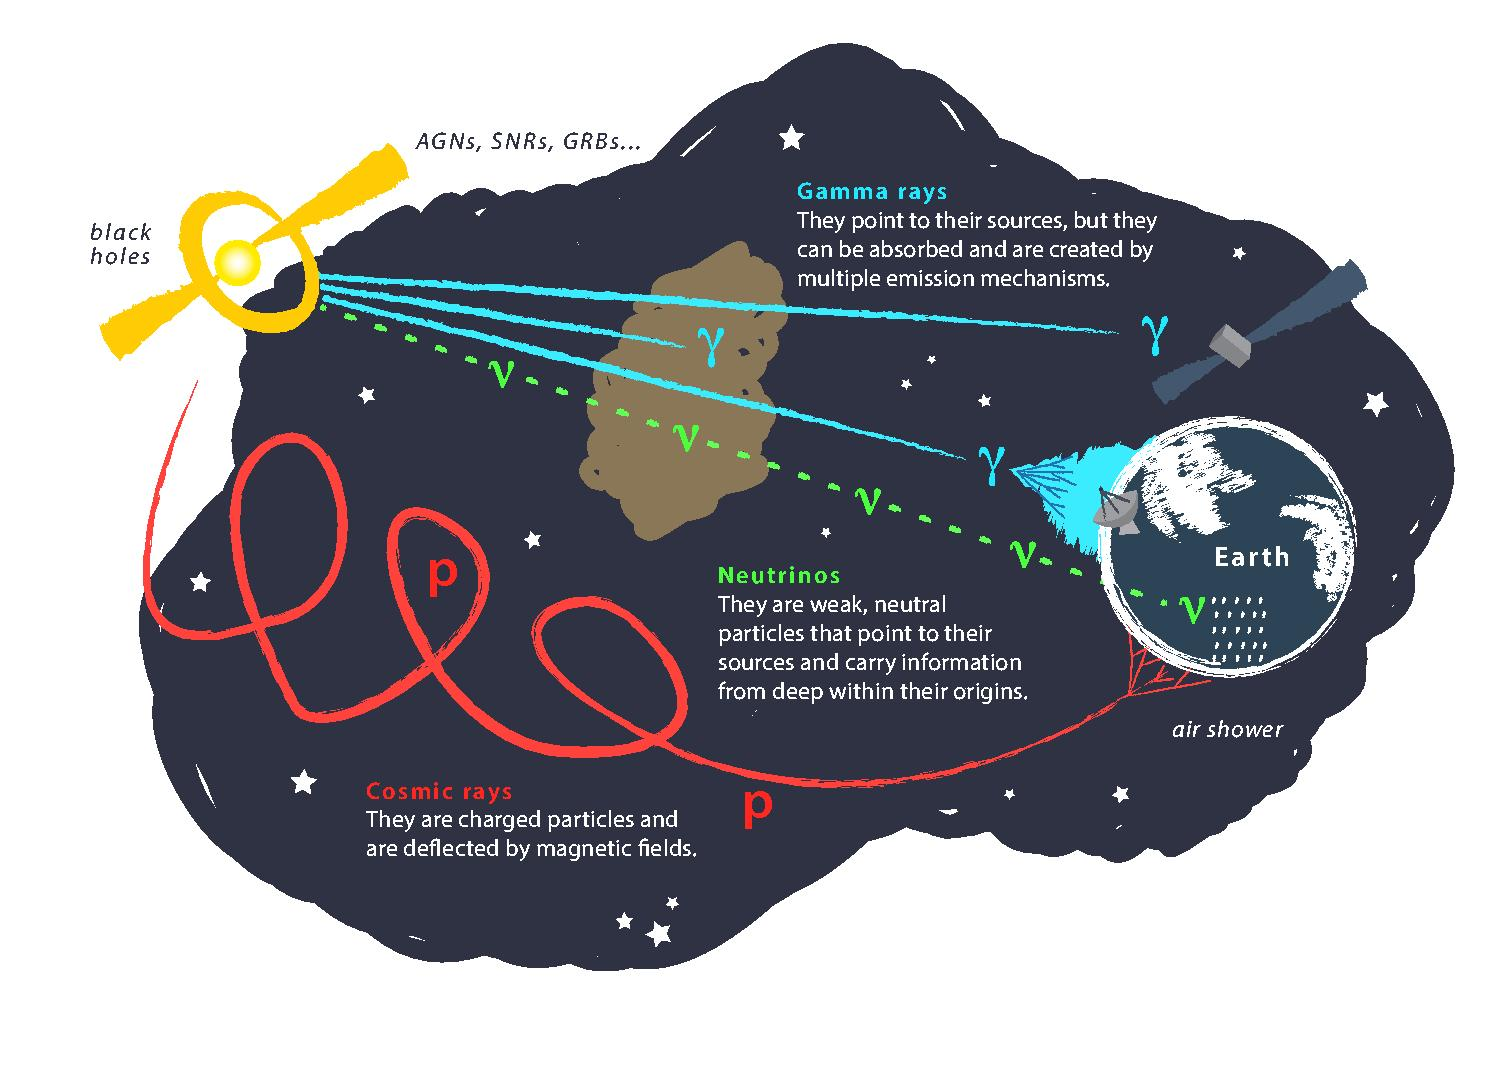
\includegraphics{mma/mm}
	\caption{An overview of multi-messenger astronomy. credit: IceCube.}
	\label{fig:mm}
\end{figure}

The existence of these high-energy charged particles \emph{cosmic rays} was first demonstrated by Victor Hess in 1912, but their origin remains unknown over a century later. In that century, the ghostly neutrino particle was first proposed by Pauli in 1930, its centrality in solar fusion was first posited by Bethe in 1939, its existence was confirmed by Cowan and Reines in 1956, the solar neutrino flux was then measured in 1964 by the Homestake with an unexpectedly-low rate (the so-called \emph{solar neutrino problem}), which then led in 2001 to the first discovery of particle physics beyond the \emph{Standard Model}, namely \emph{neutrino oscillations}. 

\begin{marginfigure}
	\centering 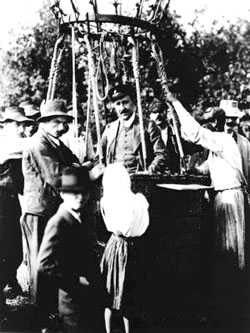
\includegraphics{intro/V-Hess-web_2.jpg}
	\caption{Victor Hess with his famous balloon, 1912. Credit?}
\end{marginfigure}

Experiments studying these solar neutrinos also accidentally provided us with the first case of observational astronomy with multiple 'messengers' (the observation of nearby supernova \emph{SN1987a} with both neutrinos and photons), followed by the discovery of extra-terrestrial high-energy \emph{astrophysical neutrinos} with the IceCube detector in 2013 produced by the very same cosmic accelerators responsible for cosmic rays. A scramble to find the origin of these neutrinos led to the birth of a new field, \emph{neutrino astronomy}. 

The long-awaited discovery of Gravitational Waves by LIGO in 2015 was shortly thereafter followed by the discovery of a Binary Neutrino Star merger, \emph{GW170817}, detected simultaneously with both photons and gravitational waves, kick-starting \emph{gravitational-wave astronomy}. One month later, the observation of a high-energy neutrino IC170922A from the direction of a flaring galactic nucleus led to the identification of the first likely source of high-energy neutrinos, \emph{TXS 0506+056}. Thirty years after \emph{SN1987a}, the year 2017 truly marked the dawn of an era of \emph{multi-messenger astronomy}. 

This thesis presents research probing the intersect of these new branches of astronomy with multiple messengers, incorporating searches for sources of neutrinos and gravitational waves using photons, and searches for photon sources using neutrinos. At its core, it seeks to understand what can be learned through combining knowledge from these new branches of astronomy with that of the oldest, namely astronomy with optical telescopes. The latter field is undergoing a revolution of its own, at the brink of transition to an algorithm-driven era dominated by enormous data volumes. Optical astronomy is moving from object-centric to population-centric science, with scales at which detailed study of individual objects is becoming infeasible. In all three fields, a focus on rapid automated responses seeks to remove human-dependent latency in observational decisions, so-called \emph{realtime astronomy}. This drive was central in the identification of both GW170817 and TXS 0506+056, and forms a central part of this work.

This thesis consists of the following chapters:

Chapter \ref{ch:theory} introduces the multiple messengers used for \emph{multi-messenger astronomy}, namely cosmic rays, neutrinos photons and gravitational waves. This chapter also introduces some of the underlying physics underpinning the emission and detection of these messengers. 

Chapter \ref{ch:sources} introduces the astrophysical populations which have been detected with multiple messengers, as well as those thought to be promising candidates for future detections.

Chapter \ref{ch:icecube} introduces the \emph{IceCube Neutrino Observatory}, located at the South Pole, and explains the detector design and operation. IceCube is the world's largest neutrino telescope, and provided data used by the author for subsequent neutrino astronomy studies.

Chapter \ref{ch:llh} explains the likelihood analysis methods used to interpret data, and to undertake searches for sources of neutrinos. As part of this thesis, the author created an open-source software package to perform likelihood analysis of IceCube data.

Chapter \ref{ch:results} outlines the results of a cross-correlation analysis, testing the hypothesis that neutrinos are produced by Tidal Disruption Events (TDEs). No signficant correlation was observed, so upper limits are derived accordingly.

Chapter \ref{ch:realtime} describes the \emph{IceCube Realtime System}, a program designed to identify probable astrophysical neutrinos with low latency and to publish the results as \emph{neutrino alerts}. Notable individual neutrino alerts are also highlighted. As part of this thesis, the author maintained this system for a period of two years. 

Chapter \ref{ch:ztf} introduces the \emph{Zwicky Transient Facility} (ZTF), an optical telescope located at Mt. Palomar, California. This telescope was used by the author to provide optical data for use in multi-messenger analysis.

Chapter \ref{ch:ztf_too} outlines the analysis pipeline developed by the author to analyse ZTF data. It further details the neutrino follow-up program operated by the author to identify optical counterparts to IceCube neutrino alerts, and highlights some results of this program. The ZTF gravitational-wave counterpart search program is also outlined, to which the author contributed substantially.

Chapter \ref{ch:bran} describes the identification of one Tidal Disruption Event, AT2019dsg, as a probable neutrino source. The multi-wavelength observations of this source are also described. This association, found by the author as part of the ZTF neutrino follow-up program, represents only the second probable association of a high-energy neutrino with an astrophysical source. It provides the first observational evidence supporting TDEs as astrophysical sources of cosmic rays.

Chapter \ref{ch:summary} summarises the main results of this thesis, and outlines the future outlook of such multi-messenger searches.




\setchapterimage[3.5cm]{mma/crab-page}
\setchapterpreamble[u]{\margintoc}
\chapter{Multi-Messenger Astronomy}
\labch{theory}
\begin{fquote}[William Shakespeare][Hamlet][1556] Though this be madness, yet there is method in it.
\end{fquote}

Multi-wavelength astronomy seeks to understand the universe through correlations between photons of different energies. Multi-messenger astronomy expands this concept to incorporate information from non-photon messengers, namely cosmic rays, gravitational waves and neutrinos. Each messenger provides a unique view of astrophysical processes in objects.

\section{Photons}

\begin{marginfigure}
	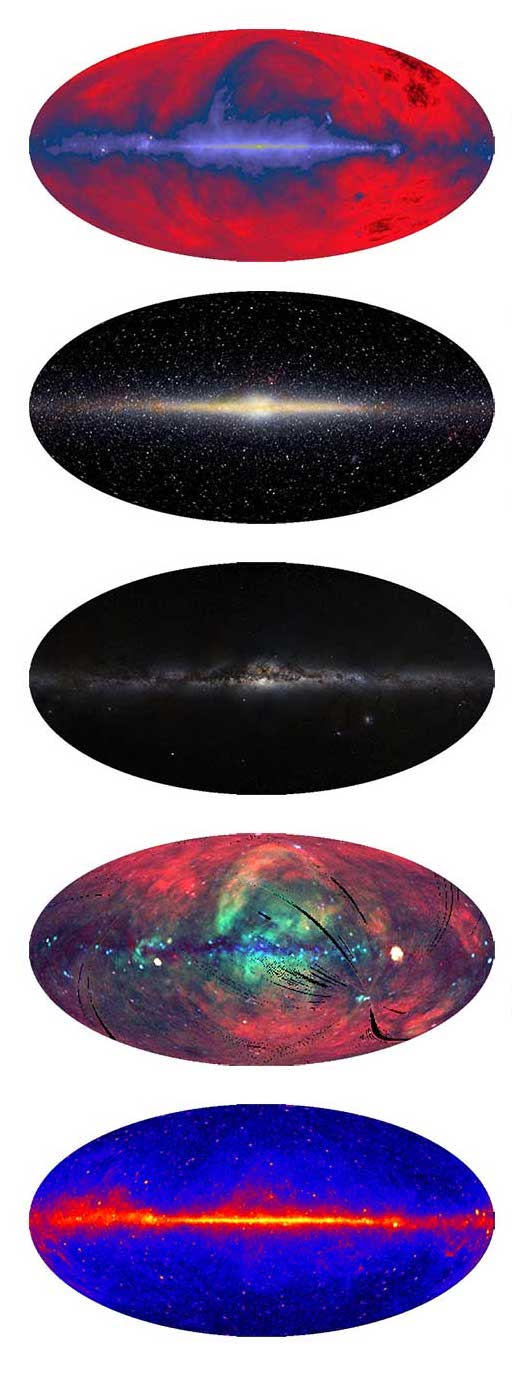
\includegraphics{mma/multiwavelength_sky_full}
	\caption{The sky, in galactic coordinates. From top: radio, infra-red, optical, X-ray and gamma-ray. Credit: NASA}
	\label{fig:mwsky}
\end{marginfigure}

Photon astronomy, in particular that in optical wavelengths, is the oldest branch of astronomy. As clear in Figure \ref{fig:mwsky}, our own galaxy is the most obvious structure at all wavelengths. The different pictures of the galaxy are also noteworthy. One example is dust extinction obscuring a large portion of the optical emission (middle panel), but  which is reprocessed to yield a particularly clear infra-red image (upper middle panel). This is an illustration of one broader principle, that interpolation between different photon energies can reveal .

In general, photon emission can be divided into two broad classes, \emph{thermal emission}
 and \emph{non-thermal emission}. Thermal emission is approximate black-bodies, and produces characteristic spectra. Non-thermal emission arises from particle acceleration, and is typically characterised by power-law emission. Objects can have both components. Thermal emission is typically centered in IR, optical or UV wavelengths, while non-thermal emission is typically manifested in both low energies (radio) and high-energies (hard X-rays and gamma-rays).
 
 \subsection*{Thermal Photons}

 \subsection*{Non-thermal Photons}
 
 \subsection*{Spectroscopy}
 
While photon observations are typically integrated over relatively-wide rsange of wavelengths, additional information can be gleaned from \emph{high-resolution spectroscopy}, in which emission in fine wavelength bins can be analysed. With precision measurements  

photoelectric effect?

\section{Cosmic Rays}

\emph{Cosmic Rays} were first discovered by Victor Hess in 1912 \sidecite{Hess:1912srp}. The name itself is a misnomer, as they are in fact charged particles. Being charged particles, they are deflected by magnetic fields, and it is thus challenging to determine where they originate from.

An industry of experiments has since developed to measure the composition and spectrum of Cosmic Rays, as illustrated in Figure \ref{fig:CR_spectrum}. The data is well-described by an unbroken power-law up to $\sim$1 PeV, beyond which there is a spectral softening known as \emph{the knee}. This softer spectrum continues before undergoing a hardening, known as the \emph{ankle}. There is then evidence of a high-energy cutoff, sometimes dubbed \emph{the second knee} in a case of metaphor-stretching.

\begin{figure}[!ht]
	\centering 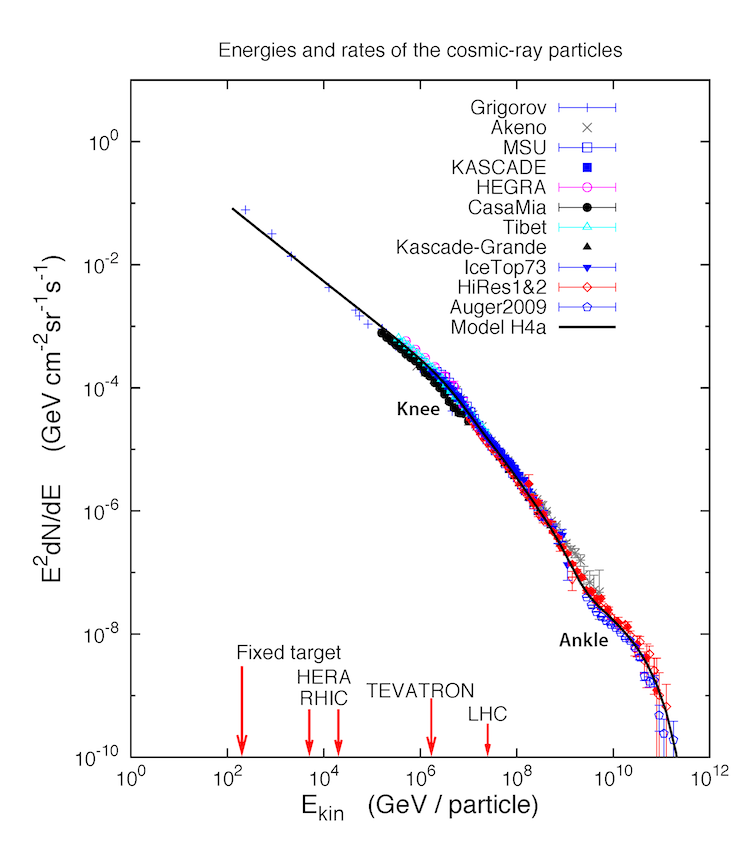
\includegraphics{mma/CRspectrum750}
	\caption{Cosmic Ray spectrum above 100 GeV, from x (icecube).}
	\label{fig:CR_spectrum}
\end{figure}

The knee is typically identified as the point at which cosmic rays transition from being predominantly galactic to extragalactic, with the ankle component being fully extragalactic. The origin of the high-energy cutoff is unclear, and the corresponding flux is so low that detector arrays must be several hundred square kilometers to study this regime with high statistics. As of 2020, this is primarily studied by the \emph{Pierre Auger Detector} and \emph {Telescope Array} detector. This regime is particularly interesting, because it is the point at which the GZK... mechanism 

UHECRs

\begin{equation}
p + \gamma_{CMB} \rightarrow \Delta^{+} \rightarrow n + \pi^{+}
\label{eq:GZK_pip}
\end{equation}
\begin{equation}
p + \gamma_{CMB} \rightarrow \Delta^{+} \rightarrow p + \pi^{0}
\label{eq:GZK_pi0}
\end{equation}

Equations \ref{eq:GZK_pip} and \ref{eq:GZK_pi0} would lead to a cutoff, in which pion production would suppress ultra-high energies above a threshold energy set by the mass of the $\Delta^{+}$ resonance. Attenuation would not occur for nearby cosmic ray sources, so the presence of such a cutoff would be evidence of an \emph{an extragalatic origin} for UHECRs. However, the \emph{Cosmic Ray Composition} determines the exact threshold for the GZK cutoff, with heavier comsic rays experiencing a much higher? threshold. There is thus much focus on understanding whether UHECRs are proton-dominated or Iron-dominated, with TA data supporting the former and PAO data supporting the latter. A joint working group concluded that these results are not in tension, once systematic uncertainties are accounted for. In summary, it appears that a definitive confirmation of a cutoff compatible with the GZK mechanism remains out of reach of present-generation instruments.

An alternative explanation for any apparent cutoff is that sources of UHECRs simply cannot accelerate particles beyond certain energies due to physical constraints. In general, any cosmic ray accelerator must at a minimum satisfy the \emph{Hillas Criterion} that any particle can be contained during the acceleration process \sidecite{1984ARA&A..22..425H}. This can be calculated by equating the Lamour Radius of a particle with the physical size of an accelerator:

Enu?

\begin{equation}
\frac{E_{\textup{max}}}{\textup{PeV}} \approx
1600 \times \frac{B}{\textup{Gauss}} \times \frac{R}{10^{16} \textup{cm}} \times
\beta Z
\label{eq:hillas}
\end{equation}

Equation \ref{eq:hillas} leads to a constraint on minimal magnetic field strength and source extension, which can be illustrated by a \emph{Hillas Plot} such as that in Figure \ref{fig:hillas_plot}. 

\begin{figure}[!ht]
	\centering 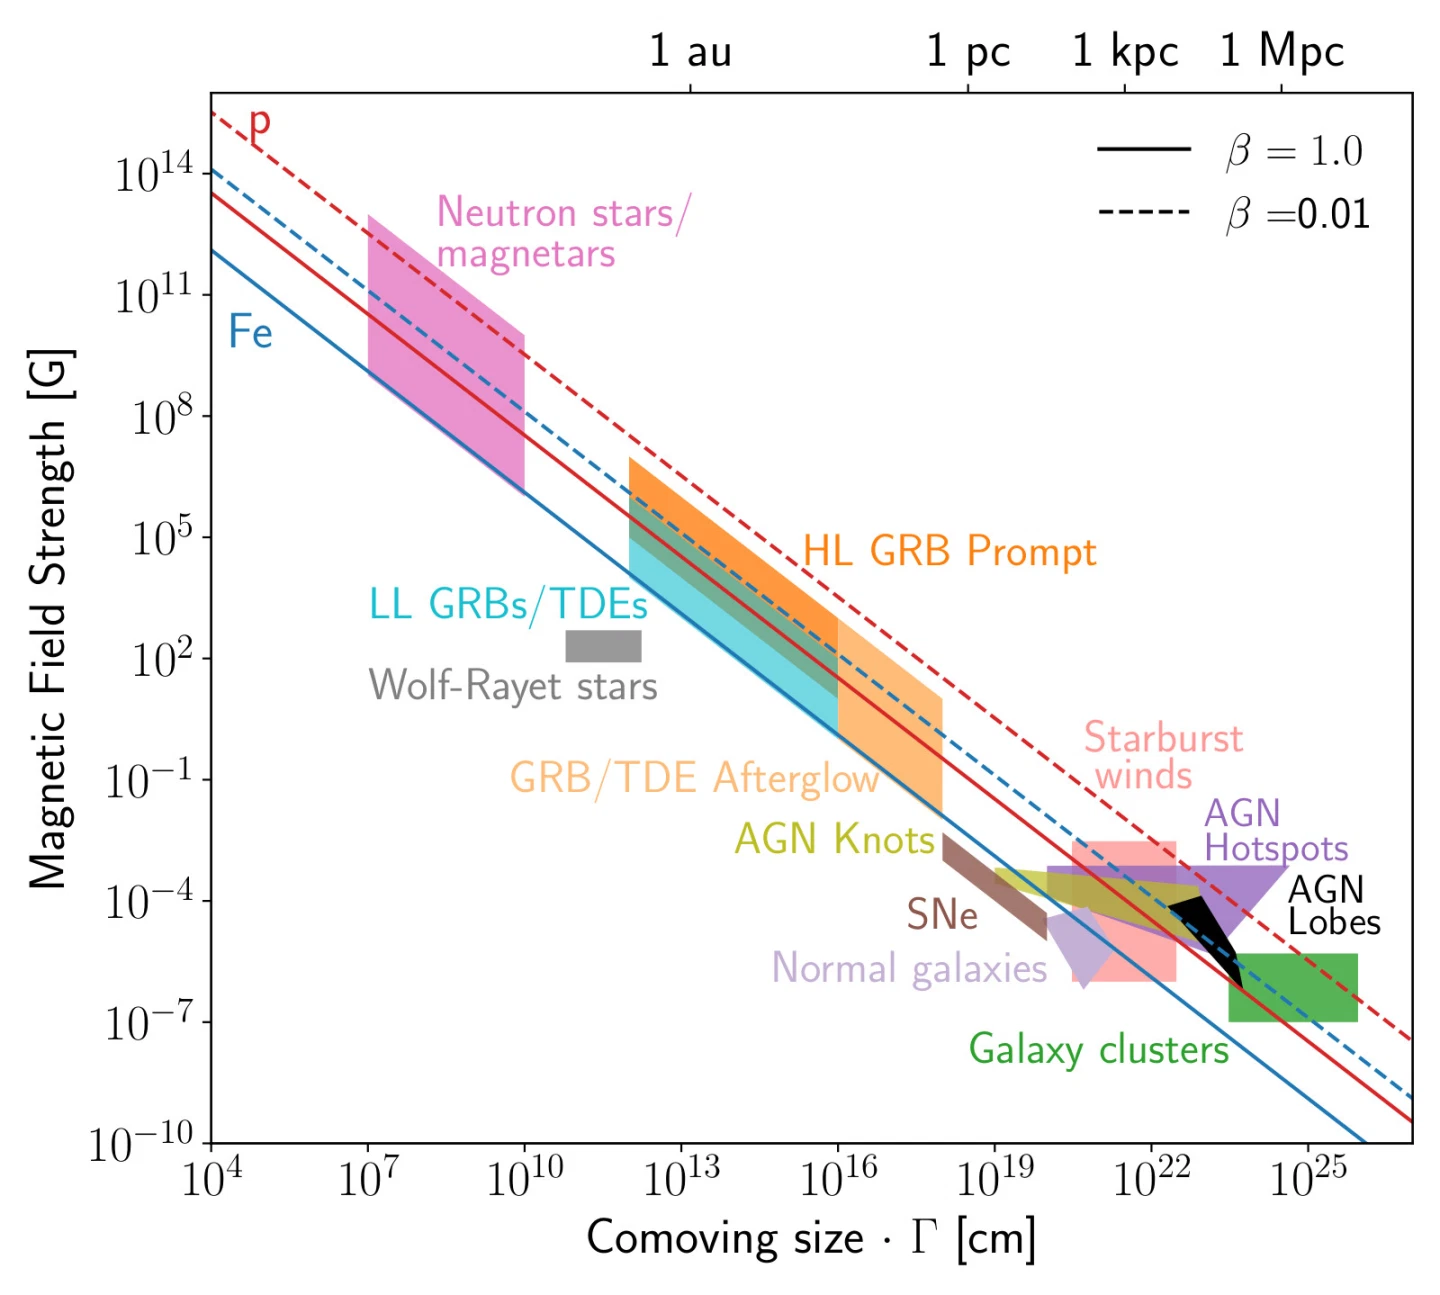
\includegraphics{mma/hillas}
	\caption{A Hillas plot illustrating possible cosmic-ray accelerators. credit: Mauricio B.}
	\label{fig:hillas_plot}
\end{figure}

The Hillas criterion \sidecite{1984ARA&A..22..425H} for a system of magnetic field strength $B$ and physical radius $R$ can be expressed as\cite{1984ARA&A..22..425H}:

\begin{equation}
\frac{E_{ \textup{max}}}{ \textup{PeV}} \approx
1600 \times \frac{B}{ \textup{Gauss}} \times \frac{R}{10^{16} \,  \textup{cm}} \times
\beta Z
\end{equation}
where $Z$ is the particle charge, $\beta \sim 0.2$ is the outflow velocity in units of c and $E$ is the maximum charged-particle energy. In order for particle acceleration to occur, the timescale required for particle acceleration must be shorter than the associated particle cooling timescale. Previous work has found this condition can be satisfied in TDEs for relevant energies\cite{2017ApJ...838....3S, 2017PhRvD..95l3001L}, although a detailed calculation is beyond the scope of this work.



Fermi acceleration

\section{Neutrinos}

The neutrino was first proposed as a particle by Pauli in 19xx as a solution to understand the mechanics of beta decay. Though observations suggested that the process involved a three-body decay, only the charged electron and proton could be measured. Invoking the existence of a light, chargeless particle provided a theoretical escape route. However, this particle was proven to be more than a theoretical construct, with the first evidence of observation by x in y.

cowan reines

DUMAND...

In parallel, the \emph{Standard Solar Model} was developed in 19xx, which correctly identified that the sun was powered by nuclear fusion. This model came with a firm prediction of a guaranteed flux of electron anti-neutrinos, \emph{solar neutrinos}, which would be produced in tandem with thermal radiation. However, the first attempt to measure the solar neutrino flux, by the Homestake experiment in 196x, found a flux that was only half the predicted level. This deficit, dubbed the \emph{solar neutrino problem}, was subsequently confirmed by many other experiments.

The solar neutrino problem was finally resolved in 200n, when the electron neutrino deficit was conclusively matched with a corresponding excess of muon neutrinos. This confirmed the presence of \emph{neutrino oscillations}, by which neutrinos can change flavour states. To undergo oscillations, neutrinos must have different non-zero mass states, in contrast to previous assumptions in the Standard Model of particle physics. 

A new generation of experiments have developed to probe neutrino flavour oscillations across a range of energies, baselines and channels. In general, \emph{reactor neutrinos} are used to probe electron neutrino disappearance, while solar neutrinos are used to probe muon neutrino appearance. Our current knowledge is summarised in N. Only the difference in squared masses can be probed by these experiments, so while it is known that mass states 1 and 2 have a difference of neV, and 13 $\sim$neV, the absolute ordering could be either \emph{Normal ordering} (m1<m2<m3) or \emph{inverted ordering} (m3<m1<m2). Directly measuring these masses remains a particle physics aim, with recent experiments such as KATRIN probing the sub-eV regime. IceCube has provided the first evidence of neutrino oscillations over astronomical baselines, with the detection of astrophysical tau neutrinos.

In 1987, experiments studying the solar neutrino problem unexpectedly measured a simultaneous excess in neutrinos. This detection occurred shortly before the discovery of a nearby supernova in the L? Magellanic Clouds, and coincided with the core-collapse of that supernova\sidecite{sn1987a_neutrino}. These \emph{supernova neutrinos} were the first that could be cleanly identified as arising from beyond our solar system, and confirmed the essential \emph{neutrino cooling} that is required during the stellar core collapse. This was also the first example of astronomy with multiple messengers. Only nearby galactic supernovae produce a sufficiently large flux to be clearly identified against this background. However, the predicted diffuse supernova neutrino background will soon be within reach of experiments.

Interactions of cosmic rays with the atmosphere produce a guaranteed flux of \emph{atmospheric neutrinos}, and this was finally confirmed observationally with the AMANDA detector in 200n. This flux extends over many orders of magnitude,. It is expected that there should be a distinct second \emph{atmospheric prompt} component of neutrinos, produced via charm quark in the atmosphere. However, this component has not yet been measured.

\emph{Astrophysical neutrinos} are to some degree guaranteed as a byproduct of high-energy cosmic ray production, resulting via pion production from the interaction of cosmic rays with ambient matter (pp) and radiation (p$\gamma$). However, the extent of astrophysical neutrino production depends very substantially on the conditions at cosmic ray accelerators, with high fluxes requiring abundant target material for pion production. A flux of astrophysical neutrinos was first discovered by IceCube in 2013, at a level close to the maximal one. This astrophysical component begins to dominate over the atmospheric neutrinos above n TeV. No neutrino source has yet been discovered, but possible sources of these astrosphysical neutrinos are discussed further in Chapter N.

At the very highest energies, it is expected that the impact of the GZK cutoff (Equations \ref{eq:GZK_pip} and \ref{eq:GZK_pi0}) should generate a flux of neutrinos through interactions of UHECRs with the cosmic microwave background. These \emph{Cosmogenic Neutrinos} have not yet been observed, but upcoming radio neutrino observatories in particular are seeking to measure them. The flux of cosmogenic neutrinos depends very strongly on the composition, density and evolution of cosmic ray sources, so it remains unclear whether it will be accessible to these detectors. (See Fig N)

\begin{figure}[!ht]
	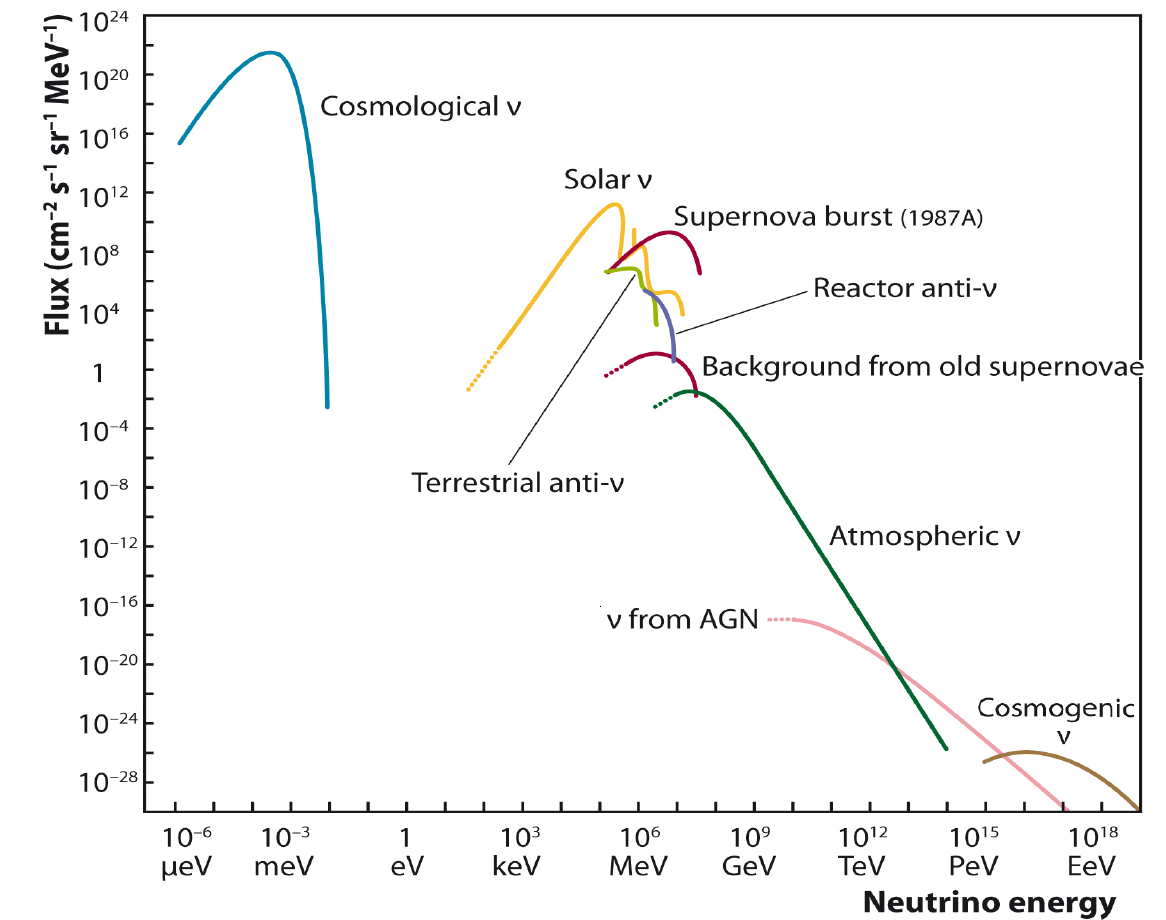
\includegraphics{mma/nu_spectrum}
	\caption{The full spectrum of neutrinos, from all sources. Credit: IceCube}
	\label{fig:nu_spectrum}
\end{figure}

\begin{figure}[!ht]
	\centering 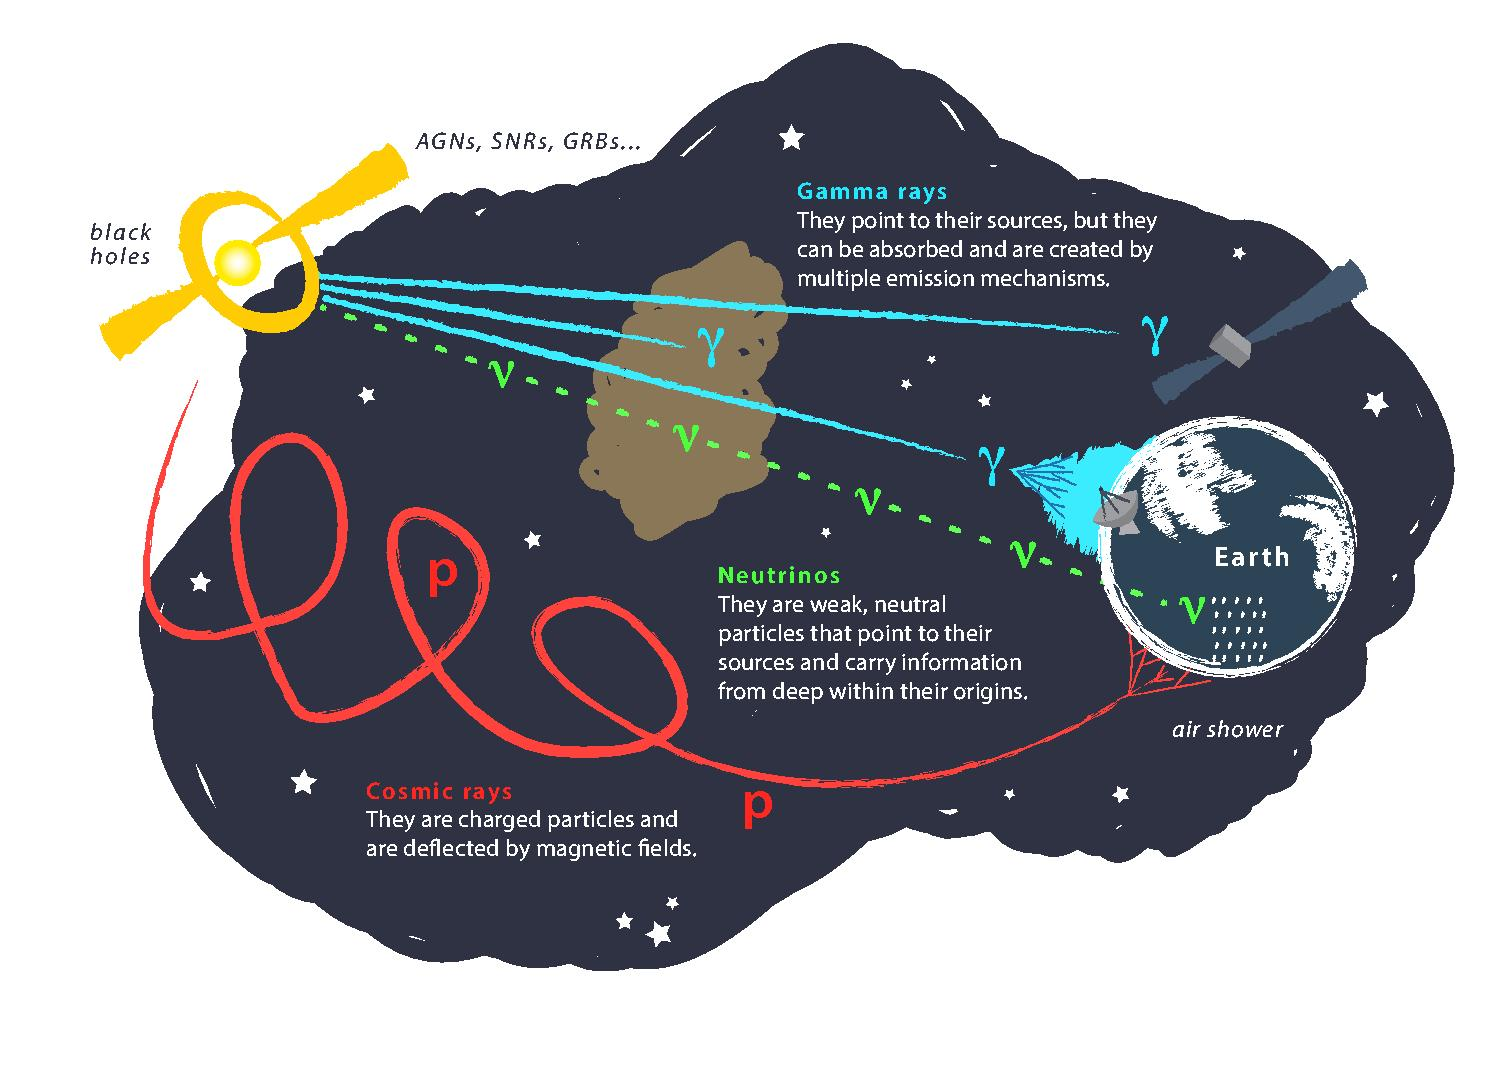
\includegraphics{mma/mm}
	\caption{An overview of multi-messenger astronomy. credit: IceCube.}
	\label{fig:mm}
\end{figure}

cosmological

In all cases, neutrino production is accompanied by a flux of pionic gamma-rays. However, these can be subsequently absorbed, so neutrinos may be produced in seemingly gamma-dark sources.

pp and p$\gamma$

For a photon target, with p$\gamma$ pion production via the $\Delta$ resonance, we expect that neutrino production will occur above the threshold introduced in Equation:

\begin{equation}
E_{\gamma}E_{p} \sim \Gamma ^{2} 0.16 \,  \textup{GeV}^{2}
\label{eq:delta_res}
\end{equation} 

Waxmann-Bachall.

glashow

MeV neutrinos from where? for ccsne
solar neutrino cycle

charged current
neutral current

\section{Gravitational Waves}

Einstein
LIGO
LISA
other sources?
quadropole moment
supernovae
Einstein Telescope
O4

The first indirect evidence for Gravitational waves came after the discovery of \emph{PSR J1915+1606}, the first pulsar binary \sidecite{hulse_taylor}. This binary system had an 8 hour orbital period that could be precisely measured in 1975, and could continue to be observed over the subsequent decades. The orbital period duration was seen to shorten over time, consistent with expectations from General Relativity for energy loss in the form of gravitational waves \sidecite{taylor_gr}. 

The arm length of gravitational waves determines 

An alternative method for direct gravitational wave detection also involves pulsars, namely the \emph{pulsar timing method} \sidecite{pulsar_gw_method}. In this case the `lever arm' is the distance to known pulsars, with passing gravitational waves being detected via the consequent deviation in pulsar cycles. The \emph{Interational Pulsar Timing Array} (IPTA) is the most comprehensive present effort to detect such emission, with sensitivity at x frequencies \sidecite{ipta}.

Recent NANOgrav results derived from pulsar timing could in principle be consistent with expectations for an astrophysical GW background, but no discovery has yet been claimed \sidecite{nanograv}.
\setchapterimage[8.5cm]{desy_blazar}
\setchapterpreamble[u]{\margintoc}
\chapter{Sources of Neutrinos and Gravitational Waves}
\labch{sources}

\begin{fquote}[Arnold J. Rimmer][Red Dwarf][1988] What the hell is a quasar?
\end{fquote}


The origin of the astrophysical neutrino flux discovered by IceCube remains unknown. In this chapter, various potential neutrino sources are discussed, as well as present constraints on the contribution of these sources. They can be broadly grouped into two classes, namely those related to the stellar life cycle and those related to supermassive black holes (see also Chapter \ref{ch:nu_cosmology}). Limits have been placed on many of these source classes by IceCube, following the procedure outlined in Chapters \ref{ch:llh} and \ref{ch:neutrino_cosmology}, but the only significant population excess found thus far has been for AGN cores.

Beyond the information presented here, new constraints placed by the author on the population contribution of Tidal Disruption Events (TDEs) and Fast Blue Optical Transients (FBOTs) are outlined in Chapter \ref{ch:results}, and the identification of the TDE \emph{AT2019dsg} as a likely high-energy neutrino source is outlined in Chapter \ref{ch:bran}.  

The origin of gravitational waves are more clearly defined, with multiple high-significance (>5$\sigma$) detections. However, there are proposed sources at frequencies other than the LIGO-Virgo-KAGRA range, which have not yet been confirmed experimentally. These are also outlined below, and summarised in Table \ref{tab:gw_source_table}. Many sources (such as supernovae) are expected to emit all four cosmic messengers.

\section{Core-Collapse Supernovae}
\label{sec:ccsn}

Supernovae, the explosive death of stars, are perhaps the best-studied phenomenon in astronomy. They are traditionally classified based on observed properties, rather than intrinsic physical attributes. An overview of a classification scheme is given in Figure \ref{fig:snzoo}. The most fundamental distinction is in explosion mechanism, with Type Ia SNe occurring due to thermonuclear explosions while all other classes are believed to arise from stellar core collapse \sidecite{sn_classification}. 

\begin{figure}[!ht]
	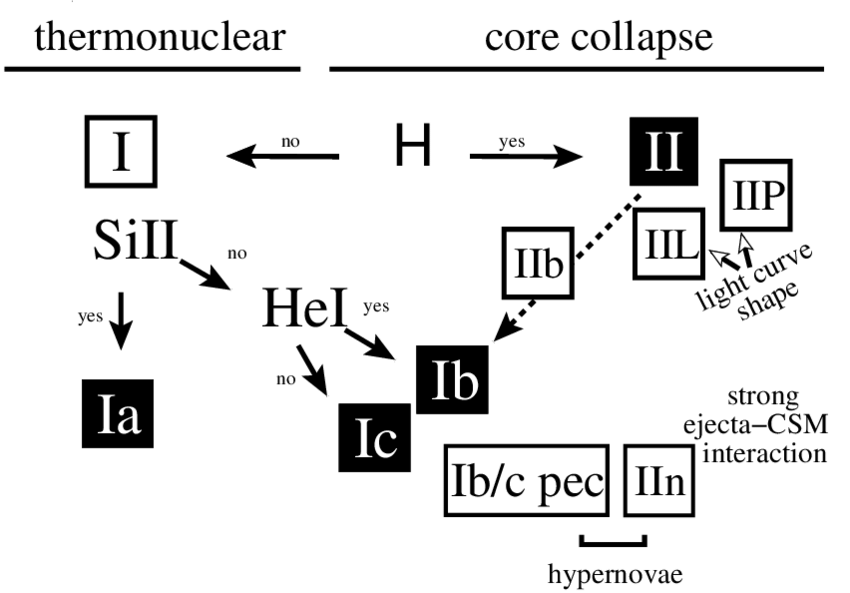
\includegraphics{sources/sn_scheme}
	\caption{An overview of the current supernova classification scheme, from \cite{sn_classification}.}
	\label{fig:snzoo}
\end{figure}

Stars begin as hydrogen gas balls, with the inward gravitational pressure balanced by the outward thermal pressure arising from hydrogen fusion. During this stage, the stellar core is gradually converted through nuclear fusion to helium until the hydrogen has been depleted. Nuclear fusion then ceases, and the decreased thermal pressure then leads to a partial collapse, at which point increased gravitational pressure increases. For massive stars, this pressure can be sufficient for helium fusion to begin. The process continues as progressively heavier elements are formed, until either the pressure is insufficient for further fusion, or up to the final iron stage beyond which fusion ceases to release net energy. Following the cessation of nuclear fusion, the lack of outward thermal pressure then causes the final \emph{stellar core collapse}.

For stars below the Chandrasekar Limit, once fusion has ceased, the gravitational compression can ultimately be balanced by the outward electron degeneracy pressure \sidecite{chandrasekar_limit}. In that case, the star will only contract until it becomes a \emph{white dwarf}, composed of electron-degenerate gas. For more massive stars, the gravitational pressure is sufficient to compress this degenerate electron gas even further, leading to \emph{electron capture} whereby protons and electrons combine to form neutrons. This leads to the formation of a \emph{neutron star}, composed of a degenerate neutron gas. The collapse launches a shock that propagates outwards through the stellar material. At the same time, the electron capture releases a burst of neutrinos, which cools the core but deposits some energy in outer layers. For extremely massive stars, this neutron star will collapse too, leading to the final stage of a \emph{stellar-mass black hole} . Either way, the neutron star formation stage leads to the phenomenon known as a \emph{supernova}, where the combination of shocks and neutrino heating expels outer layers stellar material. The rapid energy release in supernova is accompanied by substantial time-varying electromagnetic radiation, allowing superonovae to be identified via telescopes.

However, different progenitor stars and local environments leads to a considerable diversity in observational properties of supernovae. Classifications are typically made based on the presence of various spectral emission lines, but additional classifications can be made on the basis of photometric properties, such as SN IIP which exhibit lightcurve plateaus, or IIL which have linear lightcurve decays. An additional category of supernovae has been recently observed, identifiable by their atypical brightness. So-called Superluminous supernovae (SLSNe) were initially classified as any SNe with an absolute magnitude brighter than -21 mag. However, in recent years, increased study has led to a spectroscopic classification being favoured, with some dimmer objects in the range $-20 < M < -21$ also being accepted. 

\subsection*{Gravitational waves from core-collapse supernovae}

Stellar core collapse is expected to generate gravitational wave emission, in particular for cases in which the  progenitor star is rapidly rotating \sidecite{ccsn_gw}. Multi-dimensional simulations have predicted a range of different strains and frequency profiles depending on the assumed initial conditions, leaving a wide range of possible gravitational wave signatures from any nearby supernova. To date there has been no detection of gravitational waves from supernovae \sidecite{ligo_sn}. However, with the advent of more sensitive gravitational wave detectors, the next galactic supernovae may provide a novel opportunity for the first gravitational wave measurement of core collapse.

\subsection*{MeV neutrinos from core-collapse supernovae}

Since the discovery of nearby supernova \emph{SN1987A}, it has been known that neutrinos with MeV energies are produced by core-collapse supernovae \sidecite{sn1987a_neutrino}. These neutrinos are a vital component of the mechanism of stellar core collapse, and \emph{prompt neutrino burst}, followed by subsequent \emph{neutrino heating} of outer layers as energy is transferred from the core \sidecite{sn_nu_review}. Much like gravitational waves, the exact MeV neutrino emission profile will depend on the progenitor.

Though built primarily as a high-energy neutrino detector, IceCube is also sensitive to these MeV neutrinos from any nearby supernova, (see also Chapter \ref{ch:detector}). Alongside other present-day neutrino detectors, the next galactic supernova should be detected with much higher statistics than \emph{SN1987A}, enabling precise analysis of the temporal and energy distribution of the neutrino emission. They will offer an opportunity to probe physics within the core, as well as fundamental neutrino properties \cite{sn_nu_review}.

\subsection*{High-energy neutrinos from CSM-interaction}

In addition to MeV neutrinos, it has been proposed that TeV neutrinos could be produced through the collision of SN ejecta with dense circumstellar material (CSM), dubbed the \emph{CSM-interaction} mechanism \sidecite{murase_csm_sn_11}. For those SNe which occur in these dense environments, the CSM interaction typically produces characteristic spectra with narrow lines, leading to the distinct subclass of SN Type IIn. 

The timescales for neutrino production are uncertain, but could last for dozens to hundreds of days as the interaction continues. An IceCube search for neutrino emission from these Type IIn supernovae on these timescales did not reveal any significant correlation \sidecite{Stasik2018Search}, and their contribution was limited to 27.5\%  of the diffuse neutrino flux under the assumption that all IIn are neutrino standard candles. 

Supernovae of other types may also have some degree of CSM interaction, for example IIP \sidecite{iip_csm_14}. This hypothesis was also tested by IceCube, under the assumption that all IIP are neutrino standard candles, and the class was found to contribute less than n\% of the total \cite{Stasik2018Search}. This weaker constraint primarily arises from the much higher rate of IIP supernovae than IIn (see Chapter \ref{ch:nu_cosmology}). There have been no comparable studies to date on SLSNe with evidence of interaction, so their contribution remains unconstrained.

\subsection*{Supernova Jets and Long Gamma-Ray Bursts}

It is now understood that some supernovae launch relativistic jets, and that these can generate extremely luminous $\gamma$-ray transients known as Long Gamma-Ray Bursts (LGRBs), which have long been proposed as a source of neutrinos \sidecite{waxman_bahcall_97_grb}. Though these LGRBs were initially discovered independently, subsequent observations have since established that they arise from Type Ic supernova which also exhibit broad spectral lines (Ic-BL supernovae) \sidecite{98_grb_sn}. The jet itself is launched at the time of supernova explosion, leading to a GRB if aligned towards the Earth. Subsequently, a Type Ic supernova appears, with the high-velocity jet ejecta creating the characteristic broad spectral lines. However, while GRB-less Ic-BL supernovae would generally be expected due to jet misalignment, it remains unclear whether all Ic-BL supernovae launch relativistic jets or only a subset do.

In any case, neutrinos would only be expected for those jets which align towards Earth. The most reliable confirmation of an aligned jet is the corresponding detection of a LGRB, with neutrino emission typically predicted to occur during the so-called "prompt phase" of $\gamma$-ray emission (lasting $\sim$100s). 

IceCube has undertaken numerous searches for neutrino emission, but has so far observed no correlation. Owing to the similar physical conditions, these neutrino searches have often not distinguished LGRBs from the ``Short Gamma-Ray Bursts" (SGRBs) which arise from neutron star mergers (see Section \ref{sec:ns_mergers}). Prompt emission from GRBs is particularly favourable for neutrino detection, because the brief and well-defined search period greatly reduces the expected background for such searches. This scenario is indeed one of the most-constrained by IceCube, with current limits of less than 0.4\% of the astrophysical neutrino flux \sidecite{ic_grb_17}. 

\begin{figure}[!ht]
	\centering 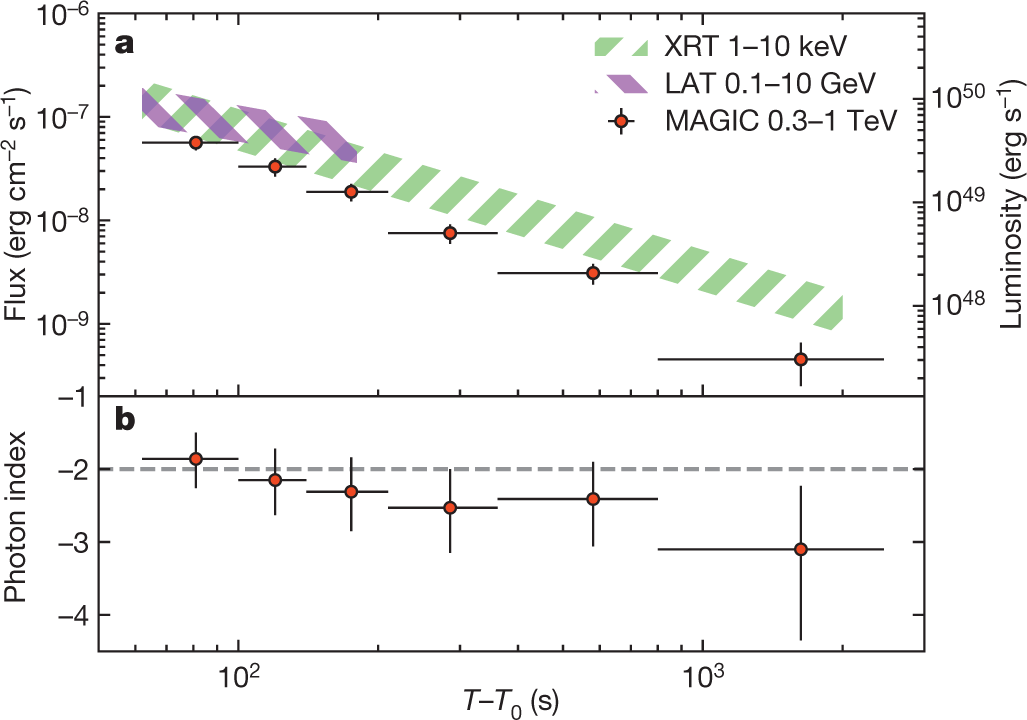
\includegraphics{sources/magic_grb}
	\caption{Detection of a GRB afterglow at TeV energies with MAGIC, from \cite{magic_grb_19}.}
	\label{fig:magic_grb}
\end{figure}

Our understanding of LGRBs has recently expanded further \sidecite{mirzoyan_grb_19}, with the discovery of VHE gamma-ray emission from a GRB reported by the MAGIC collaboration. This was followed by the announcement of a second VHE GRB detection by the HESS collaboration \sidecite{hess_grb_19}. Both were long GRBs, with the VHE detection coinciding with the well-known ``GRB afterglow" typically detected in X-ray/optical wavelengths (see Figure \ref{fig:magic_grb}). While the HESS GRB was particularly bright, the MAGIC detection was coincident with an unexceptional afterglow, suggesting that VHE emission may be common in long GRBs \sidecite{magic_grb_19}.

The timescales for this emission, extending for hours or days after the prompt phase indicates that high-energy processes extend throughout the so-called "afterglow phase". Consequently there is renewed focus on potential neutrino afterglow emission, which is significantly less-constrained. One previous Icecube analysis limited the GRB afterglow contribution to <38\% of the total \sidecite{grb_afterglow_thesis}.

\subsection*{Choked Jets and Low-Luminosity Gamma-Ray Bursts}

The same Type Ic-BL supernovae have also been associated with low-luminosity GRBs (llGRBs)  \sidecite{07_llgrb}, a distinct subclass of GRBs that are more numerous but intrinsically far dimmer than their high-luminosity counterparts. It is now thought that llGRBs arise when a jet does not successfully escape the star, but is instead smothered by the intervening material before reaching the star's surface \sidecite{nakar_15_llgrb}. Instead, a mildy relativistic shock propagates through surrounding material before ultimately reaching the surface, emitting wide-angle high-energy emission in a process known as \emph{shock breakout}. This scenario is illustrated in Figure \ref{fig:grb_diagram}.

\begin{figure}[!ht]
	\centering 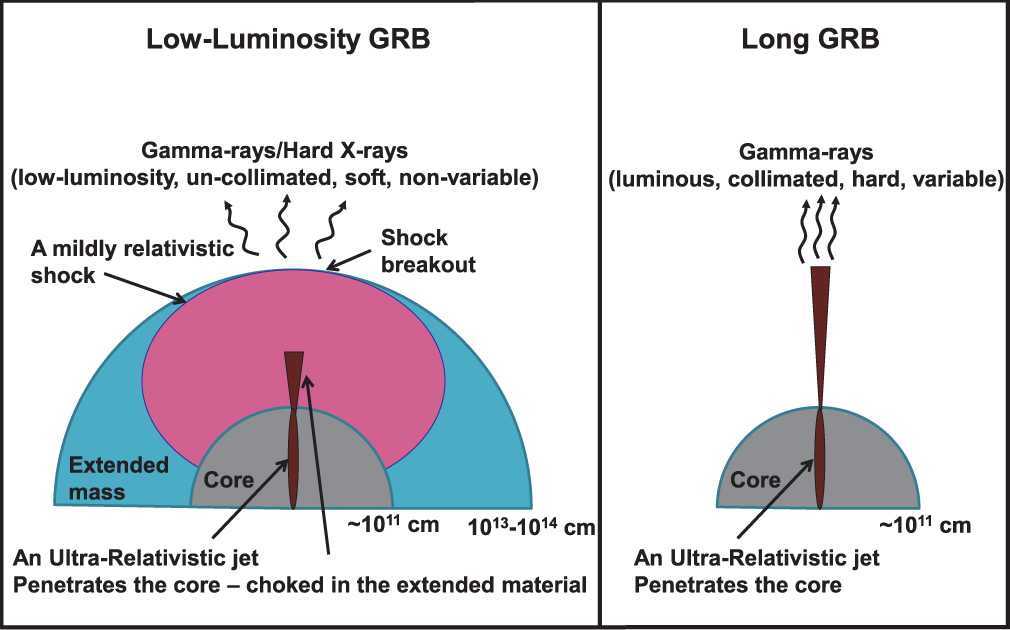
\includegraphics{sources/grb_diagram}
	\caption{Illustration of long GRBs and low-luminosity GRBs, from \cite{nakar_15_llgrb}.}
	\label{fig:grb_diagram}
\end{figure}

Though the gamma-rays are trapped, any neutrinos would still be capable of escaping the star, giving an alternative \emph{choked-jet neutrino production} mechanism \sidecite{senno_choked_jets_16}. In comparison to LGRBs, the choked jets may ultimately be brighter neutrino sources, because protons accelerated by the jet would be trapped within the envelope and efficiently produce neutrinos via pp interactions \cite{nakar_15_llgrb}. Much like for LGRBs, these neutrinos would still be expected shortly after supernova explosion, and again only if the choked jet was aligned towards Earth. However, with enhanced neutrino production and an intrinsically higher occurrence rate, llGRBs might contribute substantially more to the diffuse neutrino flux than LGRBs. 

Unfortunately, due to their low luminosity, LLGRBs are detected with much lower efficiency than LGRBs, leaving only a handful of known examples. Given this, targeted stacking searches of llGRBs are significantly less powerful. Instead, generic searches for short-scale neutrino multiplets provide constraints on the contribution of such a population. From constraints on minute-scale astrophysical neutrino clustering, assuming a GRB-like source evolution with a local rate of 325 Gpc$^{-3}$ yr$^{-1}$ for an E$^{-2.5}$ spectrum \cite{07_llgrb}, LLGRBs must contribute less than $\lesssim$20\% \sidecite{Strotjohann2020Search}.

As an alternative method, neutrinos can be directly tested for correlated with SN Ic-BL, because these supernovae are detected with much higher efficiency than LLGRBs. This scenario is however particularly difficult to test, because the alignment of a choked jet cannot be measured, so it is impossible for us to say which supernovae should or should not produce neutrinos. Furthermore, unless shock breakout is serendipitously observed, the time of supernova explosion can only be estimated to within a few days, rather than the $\sim$100s window for a GRB detection. To date, there has been no dedicated IceCube search for neutrinos correlated directly with Ic-BL supernovae. Though one study found no significant evidence of correlation with supernovae of Types Ib and Ic, that sample was dominated by non-Ic-BL supernovae \cite{Stasik2018Search}. 

\section{Stellar Remnants}

Though supernovae themselves fade on time-scales of several hundred days, they leave behind an extensive post-explosion structure that continues to be evolve over the course of millennia. There is an expanding shock front, known as a \emph{supernova remnant} (SNR), surrounding a central compact object (either a neutron star or a black hole). Post-explosion, these remnants can continue to generate multi-messenger emission in their own right.

\subsection*{Supernova Remnants}

Shocks launched by supernova explosion continue to propagate long after core collapse, leading to an expanding shock front. Alongside the central compact core, they can also host additional structure such as pulsar wind nebulae (PWNe). Multiple SNRs have been found within our galaxy, with some like \emph{Tycho's supernova remnant} being firmly associated with known historical supernova \sidecite{tycho}.

The first ever object to be detected at TeV energies was a galactic SNR known as the \emph{Crab Nebula} \sidecite{crab_whipple}, confirming that such systems can indeed accelerate particles to high energies. Many others have since been detected, making them obvious candidate neutrino sources \sidecite{gaisser_95}. IceCube has directly tested this hypothesis in various guises, with no neutrino detection yet reported. One recent example, a study of 23 young SNRs, limited the SNR catalogue contribution to less than 5.7\% of the total astrophysical neutrino flux \cite{ic_17_galactic}. SNRs themselves are not considered to be candidate gravitational wave sources, but their centrally-hosted compact remnants are promising targets (see below).

\subsection*{Neutron Stars, Pulsars and Pulsar Wind Nebulae}

Neutron stars are considered particularly promising multi-messenger sources. Due to conservation of angular momentum, the dramatic reduction in radius during core collapse means that newborn neutron stars generally rotate extremely rapidly. The rapid compression also leads to very strong magnetic fields. Due to these magnetic fields, neutron stars emit beamed radiation and accelerated particles along their magnetic poles, which need not be aligned with their axis of rotation. If this rotating beam crosses the Earth, it will be appear to observers as a lighthouse-like pulsing radio signal, leading to the name \emph{pulsar}. The first such pulsating radio signal, nicknamed \emph{LGM-1} after the ``Little Green Man" that could perhaps have sent the signal, was discovered by Jocelyn Bell Burnell in 1967 \sidecite{pulsar_hewish}. Many more pulsars have subsequently been discovered across the sky, disfavouring any alien origin for these radio signals.

These pulsars can transfer significant energy to the surrounding environment. In particular, \emph{pulsar wind nebulae} are formed due to winds launched by the central pulsar. These pulsars dominate the galactic gamma-ray sky, however the emission is thought to be largely leptonic. Nonetheless an additional hadronic contribution cannot be excluded, making pulsar wind nebulae candidate neutrino sources \sidecite{pulsar_nu_theory}.

Given the poor angular resolution of neutrino telescopes, there is substantial overlap between any SNR searches and those targeting PWNe. Beyond the generic SNR search constraints, a specific analysis targeting TeV-detected PWNe \sidecite{ic_20_pwn} constrained their contribution to less than <1.4\% of the total. 

Any aspherical pulsar could also be a source of gravitational waves, with 
the nearby \emph{Crab Pulsar} (lying within the \emph{Crab Nebula}) being one notable candidate \sidecite{gw_review}. There are dedicated LIGO searches for GWs from many different pulsars, but so far none have been detected \sidecite{ligo_pulsar}.

\subsection*{Magnetars and Fast Radio Bursts}
\label{sec:frb}

A subset of neutron stars have particularly strong magnetic fields (B $\gtrsim 5 \times 10^{13}$ G), and are known as \emph{magnetars} \sidecite{magnetar}. These magnetic fields can power dramatic electromagnetic flares on timescales of milliseconds to months, which are routinely detected at X-ray and gamma-ray wavelengths. They have also been proposed as possible neutrino sources \sidecite{zhang_neutrino_magnetar}. No dedicated search has yet been conducted targeting magnetars as a source class. Individual magnetars have been targeted by AMANDA, as well as IceCube during its construction phase, but these searches did not reveal any substantial neutrino emission \sidecite{amanda_ps}.

However, magnetars have since been linked to another astrophysical phenomenon known as \emph{Fast Radio Bursts} (FRBs). These are a class of bright millisecond radio bursts \sidecite{lorimer_07}, the vast majority of which appear to instead have an extragalactic origin. A variety of models exist to explain FRBs, but no consensus has yet emerged. The recent detection of the first galactic FRB (\emph{FRB200428}8) coincident with flaring magnetar \emph{SGR 1935+2154} confirmed that at least some FRBs are produced by magnetars \sidecite{bochenek_20}. 

Though the fluence of \emph{FRB200428} was extremely large due to its proximate origin, the intrinsic energy released was an order of magnitude lower than that of extragalactic FRBs. However, given the probable selection bias in favour of high-fluence FRBs, both \emph{FRB200428} and the extragalactic FRBs may nonetheless belong to the same underlying population \cite{bochenek_20}.

While most FRBs appear to be transient events, there are now multiple examples of repeated FRBs from the same location \sidecite{frb_repeater_16}. Repeating \emph{FRB121102} was localised to a low-metallicity dwarf galaxy, which are also known to preferentially host SLSNe and LGBRs (see Section \ref{sec:ccsn}), suggesting that these classes of transient may be connected \sidecite{petroff_frb_19}. Regardless of their origin it is clear that the detection efficiency of FRBs remains extremely low, with an estimated all-sky rate of one detectable FRB per minute, of which only a handful per year are actually detected \cite{petroff_frb_19}. 

Even before the observed magnetar association, models have suggested that FRBs may be sources of neutrinos \sidecite{frb_nu_model}. No neutrino emission was detected by IceCube for \emph{FRB200428}, strongly constraining any standard-candle FRB contribution to the diffuse neutrino flux \sidecite{ic_fra}. A significant contribution cannot be excluded for scenarios in which neutrino luminosity is not uniform across FRBs, for example if neutrino fluence were instead to scale with FRB radio fluence. Given that the detection efficiency of FRBs is so low, FRB stacking searches with IceCube have such poor sensitivity that a contribution of 100\% of the diffuse neutrino flux cannot be excluded \sidecite{ic_fra}.

Magnetars have also been proposed as possible gravitational wave sources, such as during extreme flaring periods when the magnetar may be deformed \sidecite{magnetar_gw_theory}. No emission from any magnetar has yet been detected, though the sensitivity of such searches is not sufficient to probe the expected emission \sidecite{ligo_magnetar}. The sensitivity of such searches will improve with better ground-based detectors, and will be more constraining for any nearby giant magnetar flares.

%However, because the fraction of population neutrino emission that is expected to come from detected FRBs is so low (see Chapter \ref{ch:neutrino_cosmology}), the neutrino flux contribution of the FRB population remains unconstrained \sidecite{ic_frb_20}.

\section{Compact Binaries}
\label{sec:ns_mergers}

Stellar remnants which form binary pairs can be especially promising multi-messenger sources. They are known to emit gravitational waves as the companion stars radiate energy and draw closer together, with the emitting frequency then rapidly changing in the lead up to a binary merger. By contrast neutrino emission would generally only be expected from the merger of compact binaries.

%More recently, the LIGO-Virgo Collaboration (LVC) gravitational wave detectors have recently confirmed the existence of gravitational waves through the direct detection of such binary systems \sidecite{ligo_bbh_16}. These binaries can be classified by their composition, with Binary Black Hole (BBH) mergers, Binary Neutron Stars (BNS) mergers or neutron star-black hole (NSBH) mergers. All three have now been directly detected with GW detectors.

\subsection*{Pulsar Binaries}

Pulsars can occasionally form a binary system, in which the pulsar orbits a companion star. The first such system found, \emph{PSR J1915+1606}, provided the first evidence for the existence of gravitational waves (see Chapter \ref{ch:theory}) \sidecite{taylor_gr}. The orbital period could be precisely measured due to a Doppler shift in pulsar frequency, and the expected decay in orbital period matched expectations from general relativity for gravitational wave radiation energy loss. There has so far been no direct detection of these gravitational waves because their frequency lies beyond the sensitive range of LIGO and other terrestrial detectors, but they are a prime target for longer-baseline interferometry detectors such as LISA. 

\subsection*{Binary Black Hole Mergers}

Stellar-mass black holes can also form Binary Black Hole (BBH) pairs. The existence was confirmed by the detection of a BBH merger, \emph{GW150914}, during LIGO's first observing run (O1). This same observation also provided the first direct evidence for the very existence of gravitational waves \sidecite{ligo_bbh_16}.

In general, BBH mergers themselves are not generally expected to produce either electromagnetic counterparts or neutrino emission. Particle acceleration and electromagnetic radiation could however be induced in the local environment of a merger \sidecite{murase_bbh_16}. One suggested scenario is that BBHs may preferentially form in the accretion disks of AGN, in which case shocks could generate detectable counterparts. Indeed, a candidate EM counterpart has now been reported for one of the BBH candidates reported by LIGO during O3, further supporting this theory \sidecite{graham_gw_20}.

However, a test for neutrino emission from GW triggers from the first two LIGO observing runs revealed no significant neutrino emission from BBHs \sidecite{ic_gw_20}. Given that neutrino emission would only be expected for a subset of BBH mergers, it is difficult to extrapolate from a non-detection to a limit on the overall contribution of BBH mergers to the astrophysical neutrino flux. Only the identification of electromagnetic counterpart can establish that a BBH merger belongs to this neutrino-capable subset, and no search for neutrino emission has yet been published for the sole candidate member of this class \cite{graham_gw_20}.

\subsection*{Binary Neutron Star Mergers}

Binary Neutron Stars (BNS) mergers have also been confirmed to exist, and to emit gravitational waves, following a direct detection by LIGO in 2017 \sidecite{lvc_gw170817}. The event, \emph{GW170817}, also represented the first multi-messenger gravitational wave source, because it was accompanied by the detection of electromagnetic radiation.

A Short Gamma-Ray Burst (SGRB), \emph{GRB170817A}, was detected in spatial and temporal coincidence with GW170817 \sidecite{gw170817_mm}, confirming long-standing theories that SGRBs arise from relativistic jets launched during BNS mergers \sidecite{grb_bns_92}. This coincident detection, illustrated in Figure \ref{fig:gw170817}, was followed by detections of a GRB afterglow at X-ray and radio wavelength. Ultimately these observations were jointly explained by comprehensive modelling of an off-axis jet geometry, resulting in the detection of an underluminous SGRB \sidecite{gw170817_jet_18}. Given the relatively narrow jet opening angle, it is expected that the majority of future BNS mergers detected by LIGO will not have detectable SGRB counterparts.

\begin{figure}[!ht]
	\centering 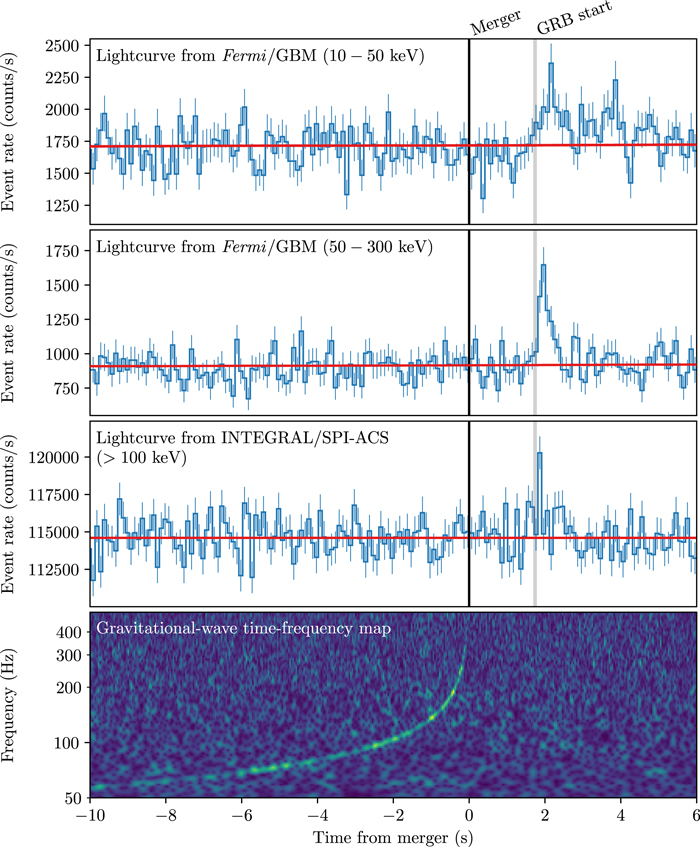
\includegraphics{intro/apjlaa920cf2_lr.jpg}
	\caption{The detection of a binary neutron star merger with photons (upper 3 panels) and gravitational waves (lower panel) , from \cite{grb170817}.}
	\label{fig:gw170817}
\end{figure}

Much like the LGRBs described in Section \ref{sec:ccsn}, SGRBs were initially identified as promising neutrino source candidates \cite{waxman_bahcall_97_grb}. However, no significant evidence for correlation has yet been found. The combined constraint on SGRBs+LGRBs, limiting their contribution to less than 0.4\% of the total diffuse neutrino flux, is the most stringent placed on neutrinos from NS mergers \cite{ic_grb_17}. An independent search for neutrino emission coincident with LIGO-detected BNS mergers also found no significant excess, though no limit was placed on the overall contribution of BNS or NSBH mergers to the diffuse neutrino flux \sidecite{icrc_hussain_19}.

A distinct second component of transient electromagnetic emission was also detected at UV, optical and infra-red wavelengths in coincidence with GW170817 \cite{gw170817_mm}. The properties of this transient, known as \emph{AT2017gfo}, matched predictions for the \emph{kilonova} that would be expected to accompany a BNS merger. AT2017gfo was thus interpreted as the first unambiguous detection of such a kilonova, with the emission arising from sub-relativistic ejecta launched during the merger. This electromagnetic signature is precisely what is targeted by follow-up searches such as that outlined in chapter \ref{ch:realtime}.

\subsection*{Neutron Star-Black Hole Mergers}

More recently, LIGO have reported the possible direct detection of Neutron Star - Black Hole mergers during their third observing run. A variety of possible production channels have been predicted, but their prevalence remains unknown. It is also unclear what multi-messenger emission might accompany such a merger, but a bright electromagnetic transient similar to that from BNS mergers might be expected \sidecite{ns_merger_counterparts}. No such counterpart has yet been detected.


\section{Tidal Disruption Events}
\label{sec:tde}

Tidal Disruption Events (TDEs) occur when a star passes close to a super-massive black hole (SMBH) \sidecite{rees_tde_88}. The strength of tidal force exerted by the SMBH on the star can exceed the self gravity holding the star together, in which case the star disintegrates, and is then said to have been \emph{tidally disrupted}. Part of the stellar debris falls back to the black hole and is ultimately accreted, a process which generates an electromagnetic signature known as a Tidal Disruption Flare (TDF).

Early modelling \sidecite{evans_89} suggested that mass fall-back rate in a TDE should follow a characteristic t$^{-5/3}$ power law, which might then lead to TDFs with corresponding t$^{-5/3}$ lightcurves. This observational signature led to the identification \sidecite{komossa_99} of the first candidate TDEs, detected in X-ray with significant transient emission. Subsequent study of TDE candidates have confirmed that mass fall-back rate is not the sole driver of emission decay, so the characteristic lightcurve decay rate will not be valid for all sources or all timescales \sidecite{auchettl_17}. TDE candidates are now more frequently identified by multi-wavelength photometric behaviour, in combination with spectroscopic observations.

The discovery of \emph{Swift J1644+57}, it is now known that some TDEs also launch relativistic jets \sidecite{bloom_11}, similar to the blazar jets introduced in Section \ref{sec:agn}. Two additional on-axis relativistic \emph{jetted TDEs} have been detected \cite{auchettl_17}, alongside one off-axis relativistic jetted TDE \sidecite{off_axis_jetted_tde}. Given this low detection rate, it is clear that jetted TDEs are particularly rare, though geometric arguments would already restrict on-axis jetted TDEs to a small fraction of the overall TDE rate.

The observational properties of TDEs are diverse. TDEs identified in optical or UV surveys are typically referred to as \emph{thermal TDEs}, because their emission at these wavelengths is often well-described by a thermal blackbody spectrum. TDEs are now commonly detected in optical surveys such as ZTF (see \ref{ch:ztf}) \sidecite{van_velzen_20}, enabling population science to be done on a homogeneous sample. Some tentative spectral classes have now been identified, analogous to those of CCSNe (see Section \ref{sec:ccsn}), which correlate to host galaxy and photometric properties of TDEs. However, systematic X-ray observations of optically-selected TDEs has revealed substantial variation in properties at keV energies, with many not detected at all \cite{van_velzen_20}. For those thermal TDEs that are detected, the X-rays emission is often itself well-described by thermal emission from a blackbody substantially smaller and hotter than for optical/UV emission. This is consistent with expectations that X-rays in TDEs typically arrive from the hot inner accretion disk. 

Radio observations have confirmed that most TDEs do not launch relativistic jets, whether on- or off-axis \sidecite{radio_tde_summary}. However, radio observations have confirmed substantial non-thermal emission from `thermal' TDEs, meaning that at least some thermal TDEs launch mildly-relativistic outflows. The presence of a central engine was inferred from observations of disk-jet coupling for thermal TDE \emph{ASASSN-14li} \sidecite{pasham_tde_diskjet}, while observations of \emph{AT2019dsg} outlined in this thesis provided the first direct evidence of a long-lived central engine in a thermal TDE (see Chapter \ref{ch:bran}).

Even before the routine detection of TDEs in sky surveys, the potential contribution of TDEs to the UHECR flux was identified \sidecite{farrar_09}. The discovery of \emph{Swift J1644+57} further expanded the possible avenues for particle acceleration in TDEs. There has consequently been much interest in TDEs as potential sources of neutrinos and cosmic rays \sidecite{Biehl_tde_uhecr}. 

As part of this thesis, the first search for neutrino emission from TDEs was undertaken (see Chapter \ref{ch:results}). The contribution of Jetted TDEs was limited to 1.3\%, while that of non-jetted TDEs was limited to 26\%.  This thesis also outlines the first observational evidence supporting TDEs as hadronic sources, with the identification of \emph{AT2019dsg} as the second likely high-energy neutrino source (see Chapter \ref{ch:Bran}), as well as the identification of \emph{AT2019fdr} as the second probable neutrino TDE (see Chapter \ref{ch:ztf}).

TDEs have also been proposed as possible sources of gravitational waves \sidecite{tde_gw}, but only at frequencies probed by future space-based missions such as LISA. Any detection would only be possible for a particularly close TDE, so it make take many years before such a joint detection is observed.

\section{Fast Blue Optical Transients}
\label{sec:fbot}

A new population of objects known as Fast Blue Optical Transients (FBOTs) has recently been identified \sidecite{drout_fbot}. While most FBOTs were detected at high redshift, interest in FBOTs has increased following the detection of a particularly nearby and bright example \emph{AT2018cow} \sidecite{Margutti:2018rri}. This promptly-identified transient at a distance of just 60 Mpc provided a rich multi-wavelength dataset, upon which most FBOT understanding is now based. The exact mechanism behind FBOTs remains open to debate, with varying interpretations such as TDEs with an Intermediate-Mass Black Hole, extreme supernovae or a magnetars \sidecite{Perley:2018oky}. In any case, they are a class of bright transients which exhibit substantial non-thermal emission, making them interesting candidates for neutrino emission.

Some degree of neutrino emission has been predicted for FBOTs, but an IceCube detection would only be expected for AT2018cow-like objects located at distances less than $\sim$15 Mpc \sidecite{fang_fbot_19}. In this thesis, the first dedicated search for neutrino emission from AT2018cow on month-long timescales was performed (see Chapter \ref{ch:results}). No significant excess was identified, and the cumulative contribution of FBOTs to the diffuse neutrino flux was limited to less than N\% of the total.

\section{Multi-Messenger Emission in the Milky Way}

As introduced in Chapter \ref{ch:theory}, the galactic plane accounts for a significant fraction of EM emission in every photon wavelength, from radio to high-energy gamma rays. It is therefore natural to suspect that the Milky Way might contribute to the astrophysical neutrino flux. Likely sources of galactic neutrinos include various stellar remnants outlined above. In addition to these steady or quasi-steady sources of galactic neutrino emission, transient sources such as core-collapse supernovae could in principle occur within our own galaxy. However, given that they are so rare, any first detection is more likely to come from local examples in the other nearby galaxies. Such transient sources are outlined in Sections \ref{sec:ccsn}, \ref{sec:frb}, \ref{sec:tde} and \ref{sec:fbot}. 

In any case, our galaxy should act as a target for extragalactic UHECRs and thus produce secondary neutrinos, it is guaranteed that some galactic contribution should be present even in the absence of galactic cosmic ray sources. However, no significant galactic neutrino excess has yet been found \sidecite{ic_17_galactic}. Given the position of the galactic centre in the southern hemisphere, where IceCube muon track datasets are less sensitive, IceCube searches are typically conducted using likely-astrophysical cascades. At this point, limits on the galactic neutrino flux are beginning to constrain reasonable models of galactic gamma-rays and CRs, including parameters of the popular KRA-$\gamma$ model \sidecite{kra_15}. Given constraints limiting the galactic contribution to less than 14\% of the diffuse flux, we can state with certainty that the astrophysical neutrino flux must be \textbf{predominantly extragalactic} \cite{ic_17_galactic}. 
%
%There are various galactic sources that could in principle produce gravitational waves, such as the Crab Nebula or binary systems, but to date none has been directly detected \sidecite{gw_review}. Pre-merger binary systems have also been known to produce gravitational waves for many decades, having indirectly provided the first evidence for the existence of gravitional waves (see Chapter \ref{ch:theory}) \sidecite{taylor_gr}. But the frequency of these waves lies beyond the sensitive range of LIGO, so a direct galactic detection would require longer-baseline interferometry detectors such as LISA. Much like neutrinos, transient gravitational waves could be found in the galaxy from sources such as compact binary mergers or supernovae, but these are infrequent occurrences.

\section{Active Galaxies}
\label{sec:agn}

Though neutrino emission from our own galaxy is limited, other galaxies may represent more promising source candidates. One long-favoured candidate neutrino source class is Active Galactic Nuclei (AGN). While most galaxies are thought to host a nuclear Supermassive Black Hole (SMBH), only a small subset of these accrete sufficient material to produce significant electromagnetic emission and qualify as \emph{Active}. As illustrated in Figure \ref{fig:agn_unification}, there are a range of observationally-defined AGN sub-classes which can be understood in the framework of the \emph{AGN Unification Model} \sidecite{2012agn..book.....B}. 

A fraction of AGN launch relativistic jets, which emit strongly at radio frequencies, and thus AGN can be divided into radio-loud or radio-quiet subsets. Radio-quiet AGN are commonly referred to as \emph{Seyfert Galaxies} \sidecite{seyfert_43}. Radio-loud AGN are subclassified as either \emph{blazars}, when observers look directly into the relativistic jet, or \emph{radio galaxies} when the jet is viewed side-on.

There are further categories based on viewing angle. The inner region of an AGN contains fast-moving gas clouds which produce Doppler-broadened emission lines, with this zone dubbed the \emph{Broad-Line Region} (BLR). This BLR is typically surrounded by a dusty torus, which can obscure the BLR when viewed side-on. For AGN where we can see broad lines in optical spectra, we classify them as either Seyfert 1 if radio-quiet, or as broad-line radio galaxies if radio-loud. Conversely, if the BLR is hidden, we have either a Seyfert 2 galaxy or a narrow-line radio galaxy (since only narrow emission lines will be visible in the spectra). Seyfert galaxies with intermediate broad-line features can be further quantified as e.g Seyfert 1.8 galaxies \sidecite{osterbrock_81}.

Distinctions of radio galaxies are also made on the basis of morphology, with the Faranoff-Riley classification scheme distinguishing those jets which become dimmer (FR-I) or brighter (FR-II) as the distance from the central AGN increases \sidecite{fanaroff_riley_74}. In general, these morphological effects are proxies for jet luminosity, with FR-II being more luminous than FR-I, hence the brighter jet extremities. Analogously, blazars can be sorted by their Spectral Energy Distribution (SED) properties into either \emph{Flat-Spectrum Radio Quasars} (high-luminosity) or \emph{BL-Lacs} (low-luminosity), with the latter class named after nearby blazar \emph{BL-Lacertae} \sidecite{95_agn_unification}.

Though AGN unification now appears natural, the historical process of discovery based on observations has left several anomalous or arbitrary classifications. Early observations of AGN identified them as compact objects of unknown origin which bore some similarity to stars. They were thus dubbed \emph{quasi-stellar objects}, or QSOs, with \emph{quasi-stellar radio objects} dubbed \emph{quasars}. 

One misfit in the standard AGN unification scheme is the phenomenon of \emph{Changing-look AGN} (CLAGN), namely those AGN which appear to rapidly transition from one class to another \sidecite{shappee_clagn}. The mechanism that causes the changing look remains unconfirmed, but explanations include variation in line-of-sight obscuration or transient accretion events such as a tidal disruption event (see section \ref{sec:tde}).

\begin{figure}[!ht]
	\centering 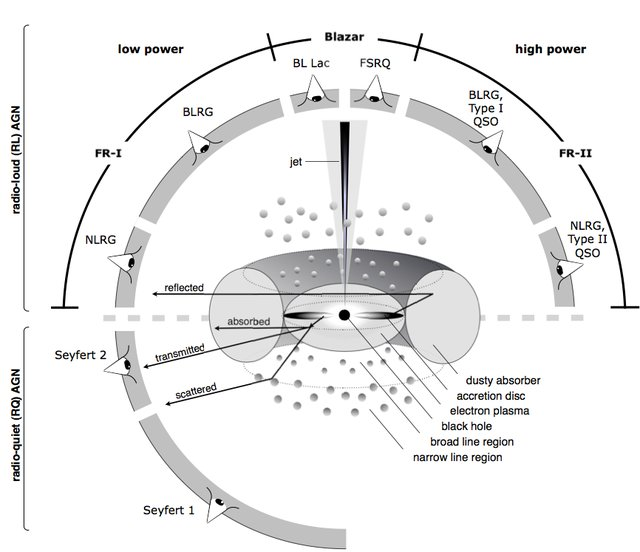
\includegraphics{sources/agn_unification}
	\caption{Unified model of AGN, with classification depending on observer viewing angle, taken from \cite{2012agn..book.....B}.}
	\label{fig:agn_unification}
\end{figure}

\subsection*{Neutrinos from Blazars}
Blazars, with their highly-beamed emission from relativistic jets, were one of the first proposed sources of high-energy neutrinos, predating the discovery of the astrophysical neutrino flux by two decades \sidecite{mannheim_93}. Blazars have SEDs with two characteristic "humps", as shown in Figure \ref{fig:blazar_sequence}. While there is consensus that the lower-energy hump likely arises from synchrotron emission,  the higher-energy one has been explained both by leptonic and hadronic models. Neutrino emission would be expected for hadronic models, though the extent would also depend on the availability of a suitable target for the accelerated hadrons to collide with.

\begin{figure}[!ht]
	\centering 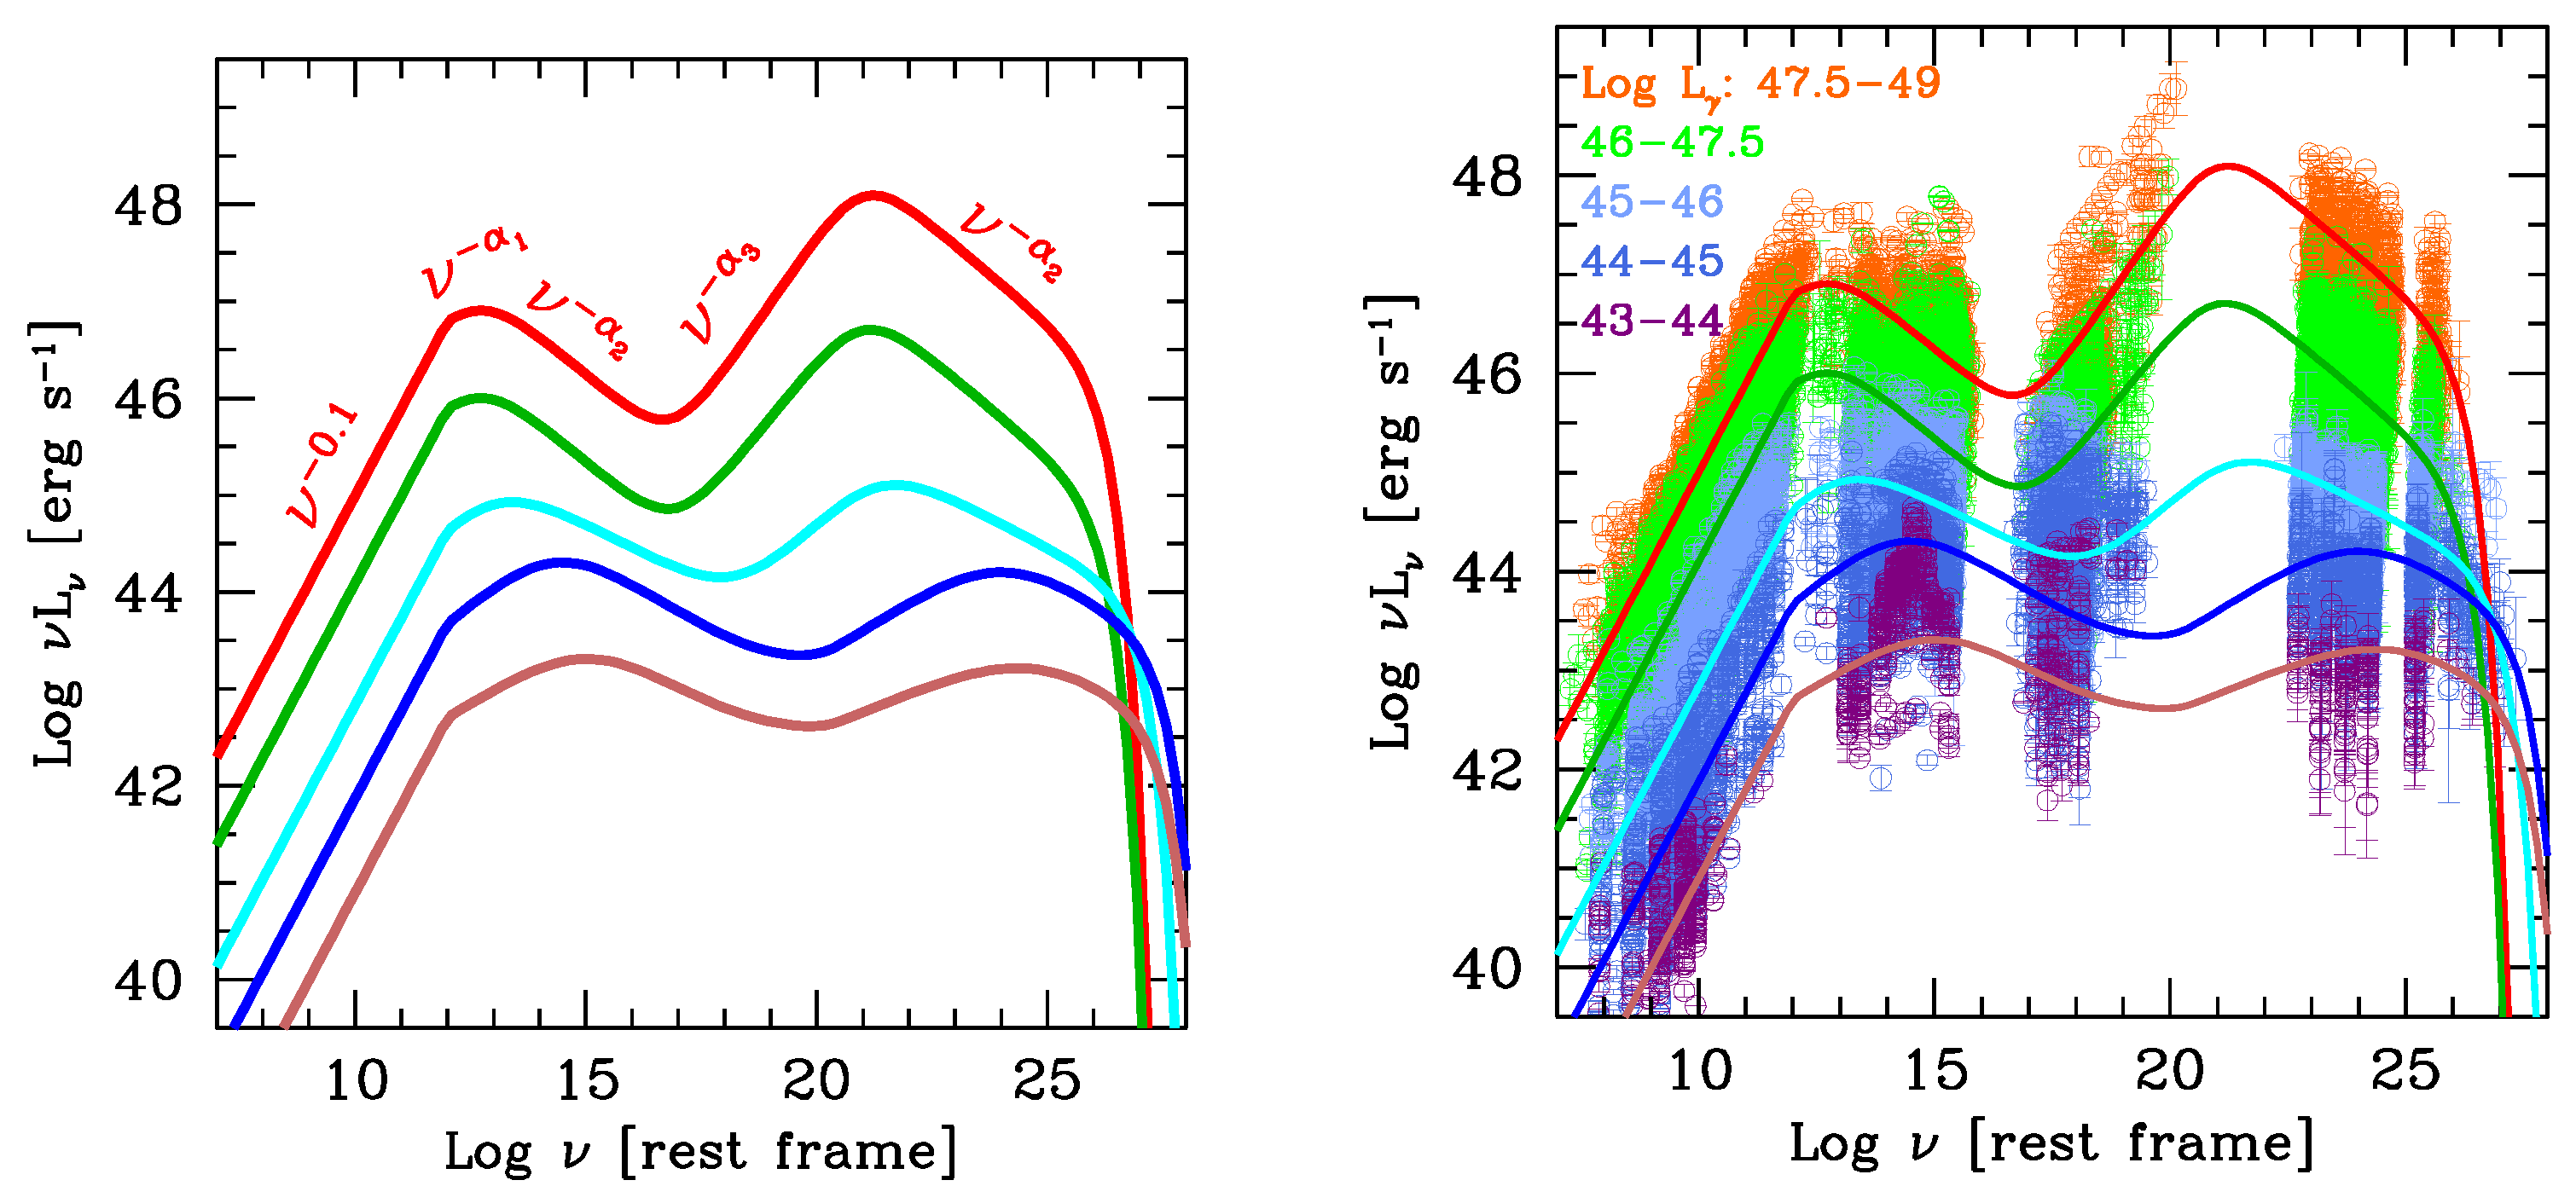
\includegraphics{sources/blazar_sequence}
	\caption{Characteristic blazar SEDs as a function of luminosity, from \cite{16_blazar_sequence}.}
	\label{fig:blazar_sequence}
\end{figure}

The second SED peak typically falls in the MeV-TeV range, and blazars are thus routinely detected by $\gamma$-ray telescopes. Since launch in 2008, the comprehensive $\gamma$-ray sky survey by the Fermi Large Area Telescope (Fermi-LAT) has now detected 3137 blazars \sidecite{fermi_4fgl}. Indeed, it is now known that blazar emission dominates the high-energy gamma-ray sky. Modelling of the "Extragalactic Gamma-Ray Background" (EGB) reveals that $\sim$ 50\% of all gamma-ray emission in the Fermi range is produced by blazars, of which $\sim$ 70\% belongs to Fermi-detected blazars \sidecite{15_fermi_egb}.  

Imaging Air Cherenkov Telescopes (IACTs) have also confirmed that blazars are extremely bright at TeV gamma-rays, beginning with \emph{Markarian 421} as the first extragalactic TeV source \sidecite{92_mrk421_tev}. However, at TeV energies and above, $\gamma$-rays are increasingly likely to interact with photons from the diffuse Extragalactic Background Light (EBL), leading to an attenuation of emission from distant objects \sidecite{10_ebl}. Though only nearby blazars can thus be detected at TeV energies, it is generally assumed by extrapolation that more distant blazars are also likely TeV-emitters.

Given the simultaneous production of gamma-rays with neutrinos in hadronic interactions, it is natural to suspect that bright gamma-ray sources, namely blazars, may additionally be neutrino sources. This hypothesis has been tested repeatedly by IceCube, and under the assumption of a linear proportionality ("$\gamma$-ray weighting"), the contribution of all blazars has been constrained to less than 10\% of the astrophysical neutrino flux \sidecite{ic_blazar_17}. Though only 862 blazars from the older Fermi 2LAC catalogue were tested, the limit is corrected to additionally account for the contribution of unresolved blazars. 

A second analysis with the same catalogue of 2LAC blazars, using an agnostic equal-weight-per-blazar assumption ("equal weighting"), found that the catalogue contributes less than 20-30\% of the total, without placing any constraint on the contribution of non-catalogue blazars \cite{ic_blazar_17}. 

More generally, the $\gamma$-ray weighting result and generic spectral considerations have \textbf{strongly constrained scenarios in which the neutrino production can be reliably traced by $\gamma$-ray emission} \sidecite{murase_hidden_sources_16}. That does not mean that blazars cannot produce a substantial neutrino flux, but $\gamma$-bright blazars must not dominate it. Recent theoretical work on blazar neutrino emission have instead focussed on evading both this and the equal-weighting constraint through models which predict a substantial contribution from unresolved and lower-luminosity blazars \sidecite{palladino_19}.

\subsection*{TXS 0506+056}

Despite these broader blazar population studies, observations of high-energy neutrino \emph{IC170922A} revealed spatial and temporal coincidence with a bright gamma-ray flare from blazar \emph{TXS 0506+056} \sidecite{2018Sci...361.1378I}, (see also Chapter \ref{ch:realtime}). A likelihood analysis correlating high-energy neutrinos with the monthly gamma-ray lightcurves of Fermi blazars led to the disfavouring of a chance coincidence at the level of $3 \sigma$. This result implied that, rather than the average gamma-ray flux, high-energy neutrinos might instead be correlated with instantaneous $\gamma$-ray blazar flux. 

Prompted by this observation, the IceCube collaboration conducted a time-dependent search for archival neutrino emission from the direction of \emph{TXS 0506+056} \sidecite{IceCube:2018cha}, and identified an additional signal-like cluster of 13 neutrinos in 2014-15 with a significance of $3.5 \sigma$. However, in contrast to the detection of \emph{IC170922A}, this "neutrino flare" was not accompanied by any significant contemporaneous gamma-ray activity \sidecite{garrappa_19}. \emph{TXS 0506+056} thus presented a somewhat contradictory picture, with both pieces of evidence challenging to interpret in a unified framework. 

Because the association of \emph{IC170922A} and \emph{TXS 0506+056} was promptly identified \sidecite{fermi_txs_atel_17}, there were extensive contemporaneous multi-wavelength observations of the flare \cite{2018Sci...361.1378I}. Theoretical attempts to model the arrival of \emph{IC170922A} generally arrived at the same conclusion, namely that without violating observational constraints the probability of detecting a neutrino alert is generally smaller than $\sim$ 15\% \sidecite{gao_txs_19}. However, this is nonetheless consistent with a physical association after accounting for the substantial Eddington Bias expected for a single neutrino detection \sidecite{2019A&A...622L...9S} (see also Chapter N).

On the other hand, attempts to model the neutrino flare were significantly more challenging because the implied neutrino flux during the flare period was extremely large. The Eddington bias should be minimal for a detection with 13 neutrinos. Despite relatively weak observational constraints for the 2014-15 period there have been no successful models capable of producing 13 neutrinos without violating the multi-wavelength observations \sidecite{rodrigues_19}.

It is difficult to simultaneously reconcile all three pieces of evidence (the stacking limit, \emph{IC170922A} and the neutrino flare). One vital question is whether \emph{TXS 0506+056} belongs to some "neutrino blazar" sub-population. The \emph{IC170922A} association can easily be reconciled once accounting for Eddington Bias from even a moderately-sized "neutrino blazar" population of $\sim$10-100 objects. However, the implied flux from the neutrino flare is so high that a similar population covering just 5\% of all blazars would already saturate the diffuse astrophysical neutrino flux \sidecite{halzen_19_txs}. In order to evade the equal-weight stacking limit, neutrino emission would also need to be heavily biased towards $\gamma$-dim blazars. The neutrino flare suggests that neutrino emission is not correlated to instantaneous gamma-ray flux. Such an interpretation is inconsistent with the original evidence to support \emph{TXS 0506+056} as a neutrino source, namely that a high-energy neutrino was detected coincident with a gamma-ray flare.

%The coincidence with a gamma-ray flare may indicate that neutrino luminosity is correlated to gamma-ray luminosity after all, but in order to reconcile a sufficient flux for neutrino alert with the the existing stacking limit, the neutrino blazar population must not include those nearby/bright $\gamma$-ray blazars which dominated the stacking limit \cite{ic_blazar_17}. Satisfying that condition, both the detection of \emph{IC170922A} and the stacking limit can clearly be understood coherently.
%
%However,understanding the neutrino flare leads to additional complications. Independent of how this implied neutrino flux is produced, it is so high that a similar population covering just 5\% of all blazars would already saturate the diffuse astrophysical neutrino flux \sidecite{halzen_19_txs}. But, in order to do so with violating the equal-weight stacking limit, neutrino emission would also need to be heavily biased towards $\gamma$-dim blazars. More generally, given that the flare was not accompanied by significant gamma-ray emission, it supports the idea that neutrino emission is not correlated to instantaneous gamma-ray flux. Such an interpretation is inconsistent with the original evidence to support \emph{TXS 0506+056} as a neutrino source, namely that a high-energy neutrino was detected coincident with a gamma-ray flare.

%Alternatively, it may be possible that one piece of evidence is somewhat incorrect or misinterpreted. The stacking limit itself may be overly conservative, because it is sensitive to the impact of unmodelled systematic uncertainties in event reconstruction (see Chapter N). Another possibility is that the timing of \emph{IC170922A} may in fact have been coincidental, while the neutrino flare may also have represented random temporal clustering. Given the degree to which searches for time-varying and steady neutrino sources are correlated, it is possible that \emph{TXS 0506+056} is instead a steady neutrino source, which by random chance exhibited some weak structure in the temporal distribution of neutrinos. One further possibility is that the neutrino flare could perhaps be a random data fluctuation, an interpretation which is supported by the lack of robustness of the excess to variations of data selection and reconstructions methods CITE.

Given the puzzling nature of \emph{TXS 0506+056}, further evidence of neutrino emission will undoubtedly be required to firmly resolve the cumulative blazar neutrino flux. In any case, \textbf{it is challenging to conceive of scenarios in which the entire astrophysical neutrino flux is produced by blazars}, leaving the door open to contributions from other source classes.

\subsection*{Neutrinos from other AGN}

Models of neutrino emission from accretion-disk shock-acceleration in AGN emerged even before those models of AGN jets \sidecite{stecker_91}. These models are generally much harder to test, because AGN are vastly more numerous than blazars, leading to a much more diffuse astrophysical neutrino flux. 

\begin{figure}[!ht]
	\centering 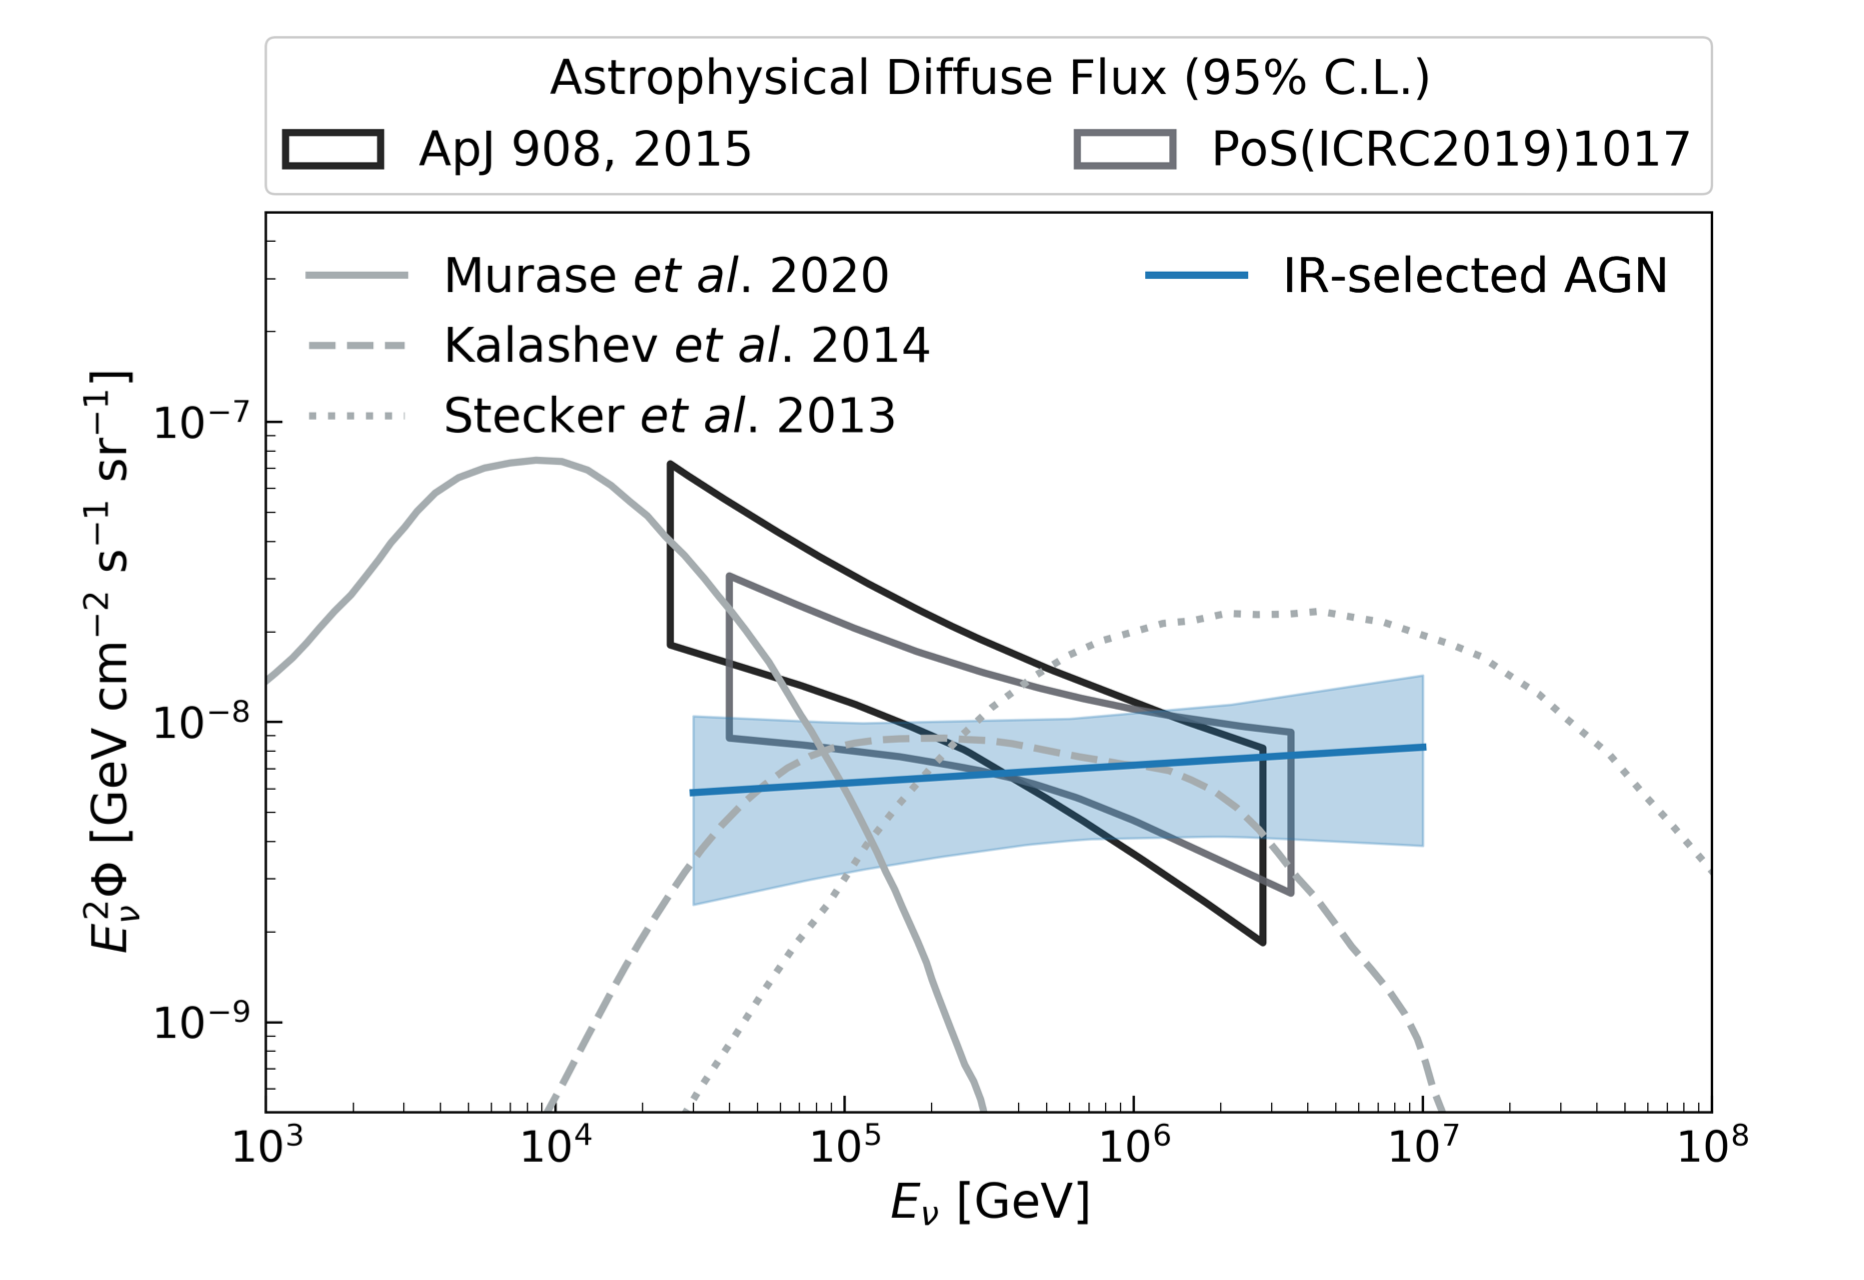
\includegraphics{sources/agn_core_flux}
	\caption{Best-fit spectrum for AGN core neutrino emission, extrapolated from a catalogue of IR-selected AGN. Figure taken from \cite{federica_thesis}.}
	\label{fig:agn_core_flux}
\end{figure}

Nonetheless, IceCube has recently tested neutrino correlations using samples of more than 30,000 radio galaxies, and identified a significant excess \sidecite{federica_thesis}. This excess was found to be robust across two catalogue compilation methods, with both results consistent in implying that \textbf{AGN cores contribute substantially to the diffuse astrophysical neutrino flux}. While most significant result is just 2.96$\sigma$ post-trial (3.16$\sigma$ pre-trial), the second catalogue has an additional pre-trial significance of 2.01$\sigma$. Though both catalogues are intended to test the same hypothesis, the source overlap is just 13\%, so that the second catalogue provides \emph{significant independent evidence supporting the association}. However, given the degree of uncertainty in the associated neutrino flux, there is plenty of scope for further neutrino flux contributions from additional neutrino sources. All catalogues favour a hard neutrino spectrum of $\gamma \approx 2$, with the implied population neutrino flux providing 28\% at 100 TeV while providing the vast majority of the neutrino at PeV+ energies.


IceCube has also recently reported that the nearby Seyfert 2 galaxy \emph{NGC 1068} had the largest neutrino excess of any tested catalogue source, with a post-trial significance of 2.9$\sigma$ \sidecite{ic_ps_10_yr}. The object, at a distance of 14 Mpc, has a high implied neutrino flux substantially above the measured gamms-ray emission. These observations can be reconciled for neutrino emission models involving the central corona, where gamma-ray absorption would obscure pionic gamma-rays \sidecite{ngc1068_theory}. If \emph{NGC 1068} is indeed an astrophysical neutrino source, the significance of the associated excess should grow steady over time as more data is collected with IceCube.

\section{Galaxy Collisions}

When two galaxies pass close to one another, the dynamics of those galaxies can change dramatically. In some cases the two pass sufficiently close to result in a direct \emph{galaxy merger}, while in other cases the two galaxies will merely interact tidally.

\begin{marginfigure}
	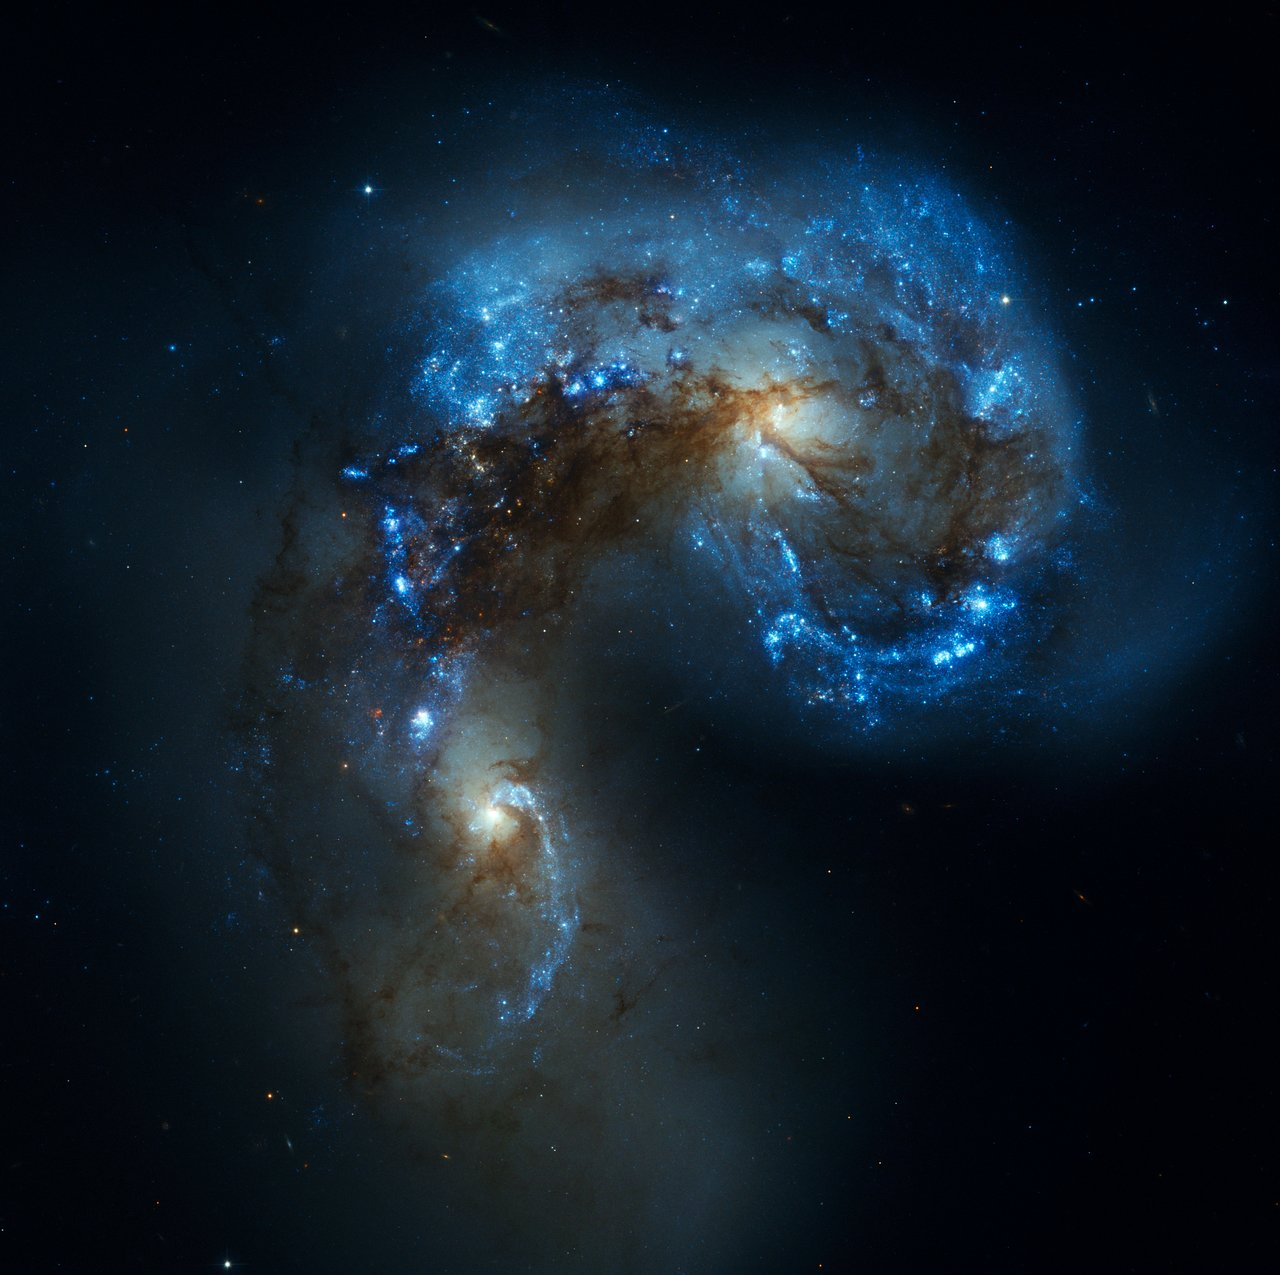
\includegraphics{sources/antenna_galaxies}
	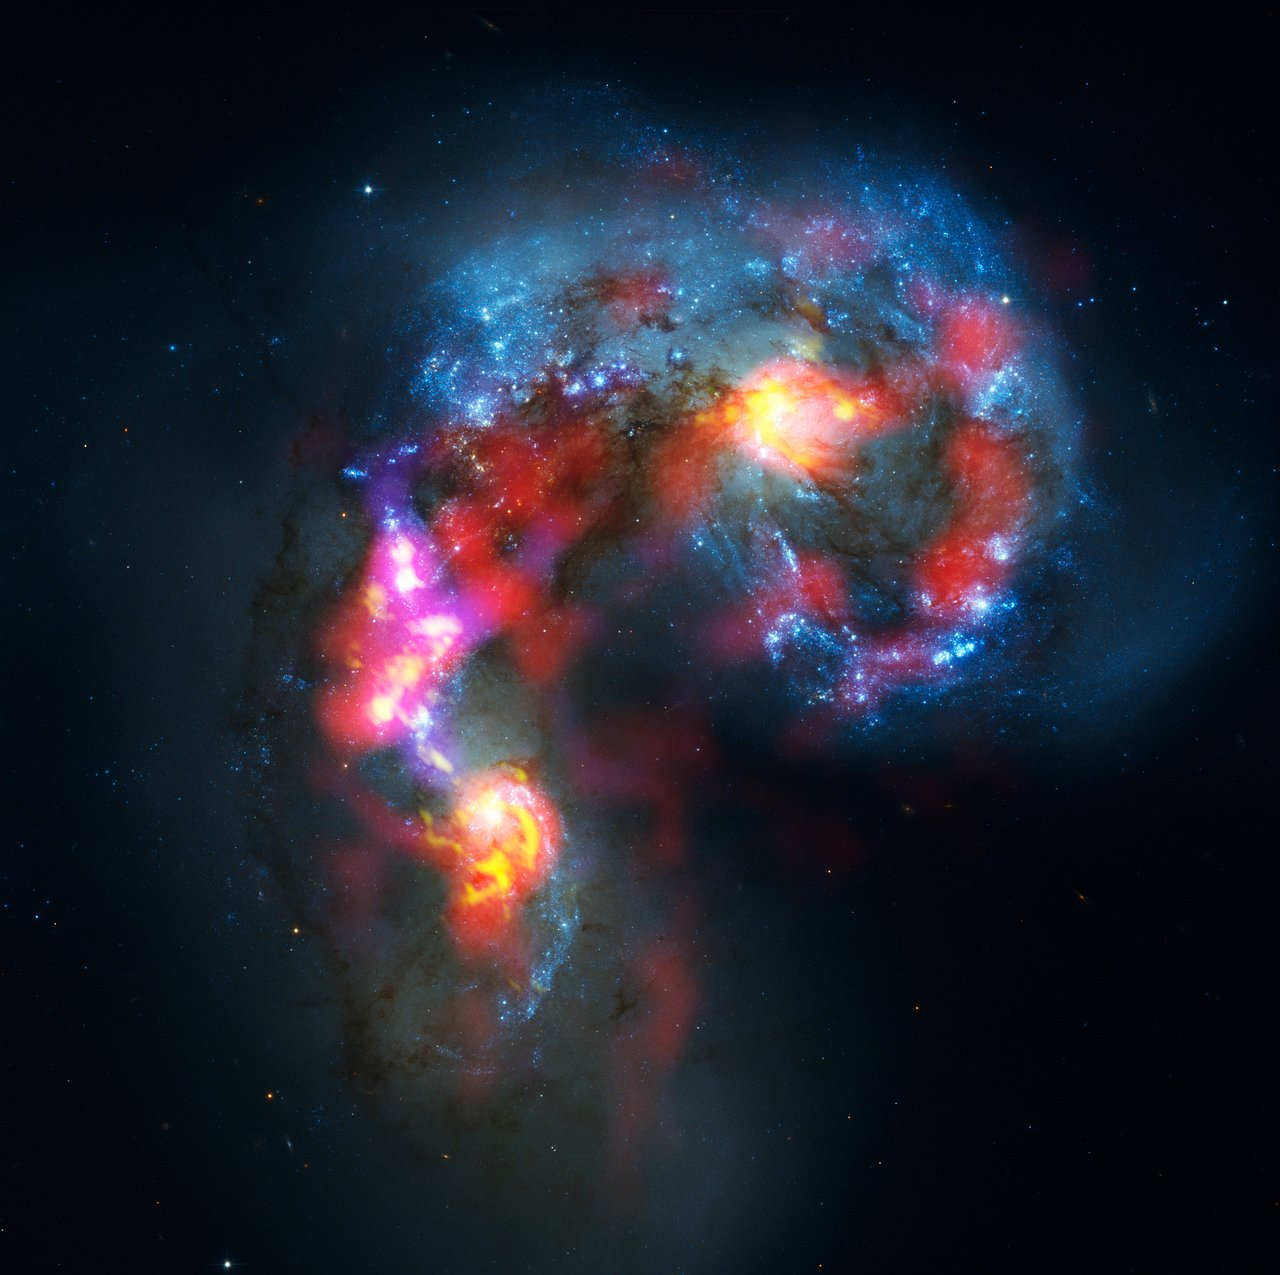
\includegraphics{sources/antenna_overlay}
	\caption{Top: The \emph{Antenna Galaxies}, with tidal interactions clearly visible. Bottom: Infra-red data is overlayed, revealing regions of high star formation. Credit: ALMA (ESO/NAOJ/NRAO), Hubble Space Telescope (NASA/ESA)}
	\label{fig:antenna_galaxy}
\end{marginfigure}

\subsection*{Starburst Galaxies}
Even without a direct merger, the impact of tidal forces from one galaxy passing close to another can induce a massive increase in the \emph{star formation rate}, by factors of 100 or 1000 (see also Chapter \ref{ch:nu_cosomology}). The star formation rate cannot be sustained indefinitely, since the raw gas is eventually depleted, but can nonetheless last for several million years. During this phase, such galaxies are referred to as \emph{starburst galaxies}, and the substantial star formation is visible via enhanced IR emission from dust heating (see Figure \ref{fig:antenna_galaxy}).

Such systems have been suggested in various models as sources of high-energy neutrinos, primarily through enhanced supernovae rates and SMBH accretion \sidecite{loeb_sbg_16}. In other words,  rather than any unique mechanism, \emph{starburst galaxies} would simply have an elevated concentration of the neutrino production processes listed in preceding sections. They would also represent a truly \textbf{diffuse} astrophysical neutrino flux. Such a scenario is unfavourable for identification against an isotropic neutrino background, and in this case it is unlikely that IceCube would have sufficient sensitivity to identify the neutrino flux origin. However, given that pionic neutrino production should be accompanied by gamma-rays, constraints can instead be derived from analysis of the non-blazar component of the gamma-ray flux \sidecite{bechtol_sbg_17}.


\subsection*{Supermassive Black Hole Binaries}

During a galaxy merger, the two supermassive black holes would eventually form a binary pair. In that case, analagous to compact binaries, these coalescing Supermassive Black Hole Binaries (SMBHBs) would be promising sources of gravitational waves  \sidecite{pulsar_gw_method}. The emission of these systems would be expected at nanohertz frequencies, and as such present a key target for pulsar timing arrays. At present there have been no claimed detections of either individual SMBHB mergers or a diffuse GW background at the relevant nanohertz frequencies. However, they remain a key science target for upcoming space-based detectors such as LISA \sidecite{lisa}.

SMBBH coalescence has also been recently proposed as possible neutrino source candidates \sidecite{nu_smbbh}, though any detection would likely require the future LISA and IceCube-Gen2 experiments. Even before coalescence, SMBBHs may have substantially elevated rates of tidal disruption events, and could thus contribute additional neutrino flux \sidecite{smbbh_tde}. 

\section{Summary}

All of these limits outlined above are listed in Table \ref{tab:source_limits}. We can also place more general constraints on different populations classes by considering a \emph{Kowalski Plot}, such as in Figure \ref{fig:kowalski_plot}, which plots an effective local density against the estimated potential neutrino luminosity for different populations. These are effective quantities because source evolution as a function of redshift must also be accounted for (see Chapter \ref{ch:neutrino_cosmology}). The diffuse astrophysical neutrino flux, as measured by IceCube, is marked with the shaded band. For any population composed of sources which are rare or dim, the expected cumulative neutrino flux will fall short of this total, so that population will only be able to contribute a fraction of the measured diffuse flux. By the same logic, for any given source density, a generic constraint on the maximum neutrino luminosity can be derived by requiring that the population emission cannot exceed the measured diffuse neutrino flux.

A separate constraint can be derived from the non-detections of bright neutrino point sources in agnostic all-sky searches \cite{ic_ps_10_yr}, which places a limit on the maximum flux of the brightest neutrino sources in any population. To evade this constraint can be achieved either by through the population flux being small, so that even the brightest sources remain sufficiently dim, or by arising from an abundant source population, so that the flux is spread across many individually-dim sources. Alternatively, source classes with positive source evolution are less constrained by these limits, as are transients. This limit is illustrated by the X region in Figure \ref{fig:kowalski_plot}, and provides more stringent constraints for rare-but-bright source classes.

The combination of these constraints, with those outlined in Table \ref{tab:source_limits}, have disfavoured most major populations as being the dominant contributors to the diffuse neutrino flux. However, this does not mean that those sources are neutrino-dark, nor that there is no prospect of neutrino source detection. It rather suggests that, much like photons, neutrinos are likely to be produced by a mixture of sources with no single population being overwhelmingly dominant. 

Gravitational wave sources are outlined in Table \ref{tab:gw_source_table}. Several classes have been directly detected, but others will need to wait for future space-based missions. For both neutrinos and gravitational waves, an element of luck is required for the detection of transient sources, because the appearance of a nearby/detectable source is an entirely random process.

\begin{table*}[]
	\centering
	\begin{tabular}{|c c c c c c|} 
		\hline
		Source Class & Limit Type & Fraction & $\phi_{0}$ at 100 TeV & Weighting & Reference\\ 
		&&[\%]&[GeV$^{-1}$ cm$^{-2}$ s$^{-1}$]&&\\
		\hline
		SN IIn & Population & <27.5 & <7.7 $\times 10^{-18}$&Standard Candle&\cite{Stasik2018Search}\\
		SGRB+LGRB (Prompt) & Population & <0.4 &$\lesssim$1.0 $\times 10^{-19}$&Equal&\cite{ic_grb_17, maunu_thesis}\\
		SN Ib+Ic & Population & <12.8 &<3.6 $\times 10^{-18}$&Standard Candle&\cite{Stasik2018Search}\\
		LLGRBs & Population & $\lesssim$20 &$\lesssim$5.6 $\times 10^{-18}$&Standard Candle&\cite{Strotjohann2020Search}\\
		SNR (TeV-detected) & Catalogue & <5.7 & <1.6  $\times 10^{-18}$ & Equal & \cite{ic_17_galactic}\\
		PWN (TeV-detected) & Catalogue & <1.4 & <4.5 $\times 10^{-19}$ & Equal &  \cite{ic_20_pwn}\\
		FRB & Population & <0.3 & <8.4 $\times 10^{-20}$& Standard Candle & \cite{ic_fra}\\
		FRB & Population &  $\leq$100.0& $\leq$2.8$\times 10^{-17}$& E$_{\nu} \propto$ E$_{radio}$& \cite{ic_fra}\\
		TDE (Jetted) &Population& <1.3& ???&Standard Candle & This work\\
		TDE (Non-jetted) & Population &<26.& ???&Standard Candle & This work\\
		FBOT & Population & < ???? & ??? & Standard Candle & This work\\
		Galactic Plane & - & <14.0 &  <3.8 $\times 10^{-18}$  & Fermi-LAT $\pi_{0}$ model &\cite{ic_17_galactic}\\
		Blazar (Fermi-detected) & Catalogue & <27.0 & <7.6 $\times 10^{-18}$& Equal & \cite{ic_blazar_17}\\
		Blazar (all) & Population &<10.0&<2.8 $\times 10^{-18}$& L$_{\nu} \propto$ L$_{\gamma}$& \cite{ic_blazar_17}\\
		AGN Cores & Population &\sim28 &\sim 7.9 \times 10$^{-18}$& L$_{\nu} \propto$ L$_{x}$&\cite{federica_thesis}\\
		Starburst Galaxies & Population &<30.0& <8.4 $\times 10^{-18}$ & L$_{\nu} \propto$ L$_{\gamma}$&\cite{bechtol_sbg_17}\\
		\hline
	\end{tabular}
	\caption{Summary of the limits on each neutrino source class, including results from Chapter \ref{ch:results}. Those limits marked \emph{Population} represent limits on the total contribution of a source class, while \emph{Catalogue} limits constrain only those sources tested. Fractions are given as a percentage of the combined neutrino+anti-neutrino diffuse flux measured in \cite{ic_global_fit_15}, with sky-integrated per-flavour normalisation of 2.81 $\times 10^{-17}$ GeV$^{-1}$ cm$^{-2}$ s$^{-1}$ at 100 TeV, and spectral index $\gamma=2.5$}
	\label{tab:source_limits}
\end{table*}{}

\begin{figure}[!ht]
	\centering 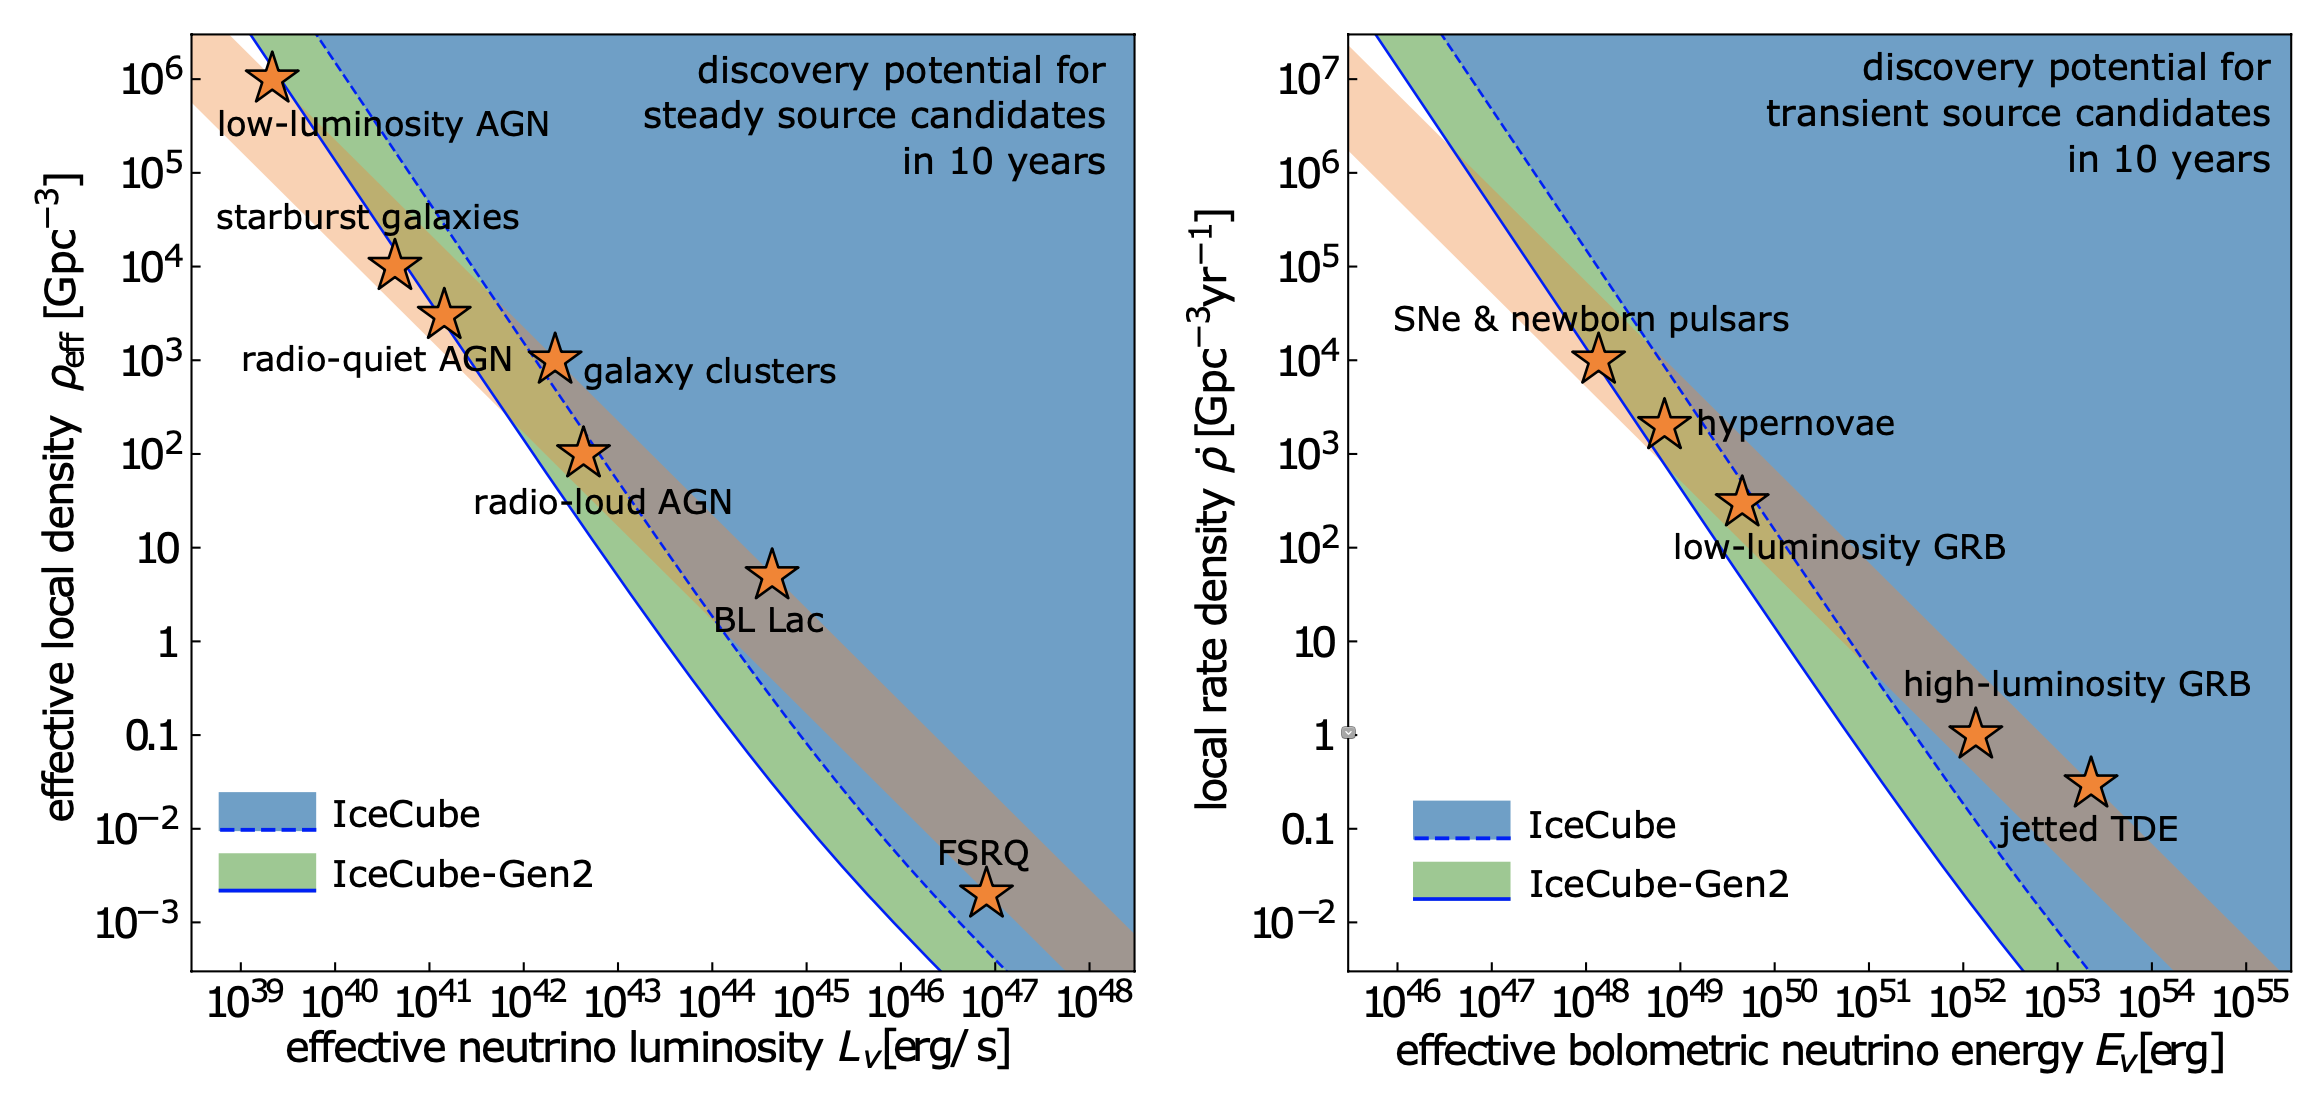
\includegraphics{sources/kowalski_plot}
	\caption{\emph{Kowalski Plot} illustrating source densities and luminosities, from \cite{ic_gen2_20}.}
	\label{fig:kowalski_plot}
\end{figure}

\begin{table*}[]
	\centering
	\begin{tabular}{| c c c c |} 
		\hline
		Source Class & Frequency & Directly Detected? & Indirectly Detected? \\ 
		\hline
		CCSN &Hz-kHz&\xmark&\xmark\\
		Pulsar &Hz-kHz &\xmark&\xmark\\
		Magnetar & Hz-kHz &\xmark&\xmark\\
		Pulsar Binary &\sim10$^{1}$???&\xmark&\textcolor{ForestGreen}{\cmark}\\
		BBH Merger &Hz-kHz&\textcolor{ForestGreen}{\cmark}&\xmark\\
		BNS Merger &Hz-kHz&\textcolor{ForestGreen}{\cmark}&\xmark\\
		NSBH Merger &Hz-kHz&\textcolor{ForestGreen}{\cmark}&\xmark\\
		TDE&mHz&\xmark&\xmark\\
		SMBBH (Inspiral) & nHz &\xmark&\xmark\\
		SMBBH Merger & mHz &\xmark&\xmark\\
		\hline
	\end{tabular}
	\caption{Summary of each GW source class.}
	\label{tab:gw_source_table}
\end{table*}{}

% Icecube

\pagelayout{wide} % No margins
\addpart{Neutrino Astronomy with IceCube}
\pagelayout{margin} % Restore margins

%
\setchapterimage[6.5cm]{icecube}
\setchapterpreamble[u]{\margintoc}
\chapter{IceCube Neutrino Observatory}
\labch{icecube}
\begin{fquote}[Edmund Hillary][][1957] I am hell-bent for the South Pole — God willing and crevasses permitting.
\end{fquote}
The IceCube Neutrino Observatory is the world's largest neutrino telescope, located at the geographic south pole. It was built as a successor to the AMANDA experiment, which had pioneered the detection of neutrinos in ice. AMANDA served as a proof of concept for the detection of neutrinos, but with a volume of just nkm$^{3}$, it only had sufficient effective area to measure atmospheric neutrinos. 

IceCube, on the other hand, was envisioned as a much larger detector capable of measuring astrophysical neutrinos. It was constructed in phases from 2006 to 2011, eventually reaching a total volume of one cubic kilometer. 

\section{The IceCube Detector}

IceCube is composed of 86 strings arranged in a hexagonal grid. Each string is 2.5 km long, and carries regularly-spaced Digital Optical Modules (DOMs) containing Photo-Multiplier Tubes (PMTs). With a hot-water drill, holes were drilled into the glacier ice to a depth of 2.5 km. After string deployment, the liquid-filled holes refroze, fixing the DOMs in place. In total, there are 5160 DOMs deployed in IceCube, all at depths greater than 1km. The Antartic ice itself thus provides the detection medium for neutrinos, with the Earth acting as a shield against atmospheric muons.

The design of IceCube is an optimisation trading DOM-density against effective area for fixed cost. A minimal DOM density is needed to identify and reconstruct an event, and this threshold decreases as neutrino energy increases. Thus, while IceCube is generally optimised for detecting high-energy neutrinos in the astrophysical regime, it is far too sparse to effectively measure lower-energy (1-100 GeV) neutrinos. However, in addition to the regular grid of strings, IceCube contains a denser in-fill array known as \textit{Deepcore}. This array consists of 7 strings and n DOMs, and typically uses the outer IceCube detector as a veto against muons?. \textit{Deepcore} measures low-energy neutrinos which form the basis of neutrino oscillation studies, but can also be used for neutrino astronomy at lower energy scales.

IceCube also contains a surface array of instrumented ice tanks known as IceTop, which are used to measure surface air showers arising from cosmic rays and photon interactions. IceTop can be used as a veto against muons from air showers, but only for a small fraction of events which are almost-vertically down-going. However, IceTop also functions in its own right as a Cosmic-Ray detector, and contributes competitive measurements of the cosmic ray flux and composition.

While most event selections for GeV and TeV-PeV neutrinos require multiple DOM hits to reject thermal-noise background, a separate detection channel exists for MeV neutrinos that are typically produced in both stellar fusion and supernova collapse. These neutrinos form an irreducible background for the IceCbe detector, with extremely short track lengths that are only detectable by single DOMs. A dedicated SuperNova Data Aquistion System (SNDAQ) is installed to measure the rate of these single-DOM detections, and identify any significant deviation from expected rates. As demonstrated by SN1987a, any nearby supernova will produce a significant flux of MeV neutrinos during core collapse, and this will be manifested in a significant uptick in trigger rate that will evolve as a function of time. It is predicted that IceCube will be able to clearly measure the temporal evolution of MeV neutrinos from any supernova in the galaxy or Magellanic Clouds, similar to Figure NNNN. IceCube sends any mid-significance deviations from trigger rate to the SuperNova Early Warning System (SNEWS), where they are cross-correlated with other sensitive neutrino detectors such as SNO and Super-K. In the event of a multi-detector trigger, observatories around the world will be alerted to the upcoming optical counterpart of a galactic supernova, which can be localised in the case of a strong signal by combining directional information from individual detectors and time-delays between detectors in differing geographical locations. 



MeV neutrinos for supernovae.

\section{Proposed Improvements to the IceCube detector}

There are several planned or proposed extensions to IceCube that would substantially improve the detector performance. Beginning in 2023, deployment will start for the IceCube Upgrade, a Deepcore-like dense infill array. The string spacing will be even tigher than deepcore, with a higher density of DOMs. In combination with hardware improvements from multi-PMT DOMs, the Upgrade should push IceCube's lower energy threshold from a few GeV, and potentially to below one GeV. This opens up an entirely new regime for both oscillation studies and lower-energy neutrino astronomy relative to competitor neutrino detectors such as SuperK. In addition to the gains from DOMs, many new calibration devices will be deployed to more accurately constrain sources of systematic uncertainties, in particular the ice scattering and absorption length. With these calibration measurements, archival neutrino data can be reprocessed, providing more accurate reconstructed parameters. Improvement should be expected for all neutrino sources analyses, which all suffer to lesser or greater degree from these systematic errors. 

Beyond the IceCube Upgrade, a more comprehensive improvement is planned to extend the higher-energy capability of IceCube. IceCube-Gen2 is a proposed extension instrumenting 10 km$^{3}$ of ice, with a sparser string footprint than the existing detector. While multi-PMT DOMs should partially compensate the lower density, Gen2 represents a transition in focus to higher-energy neutrinos at 10TeV-100PeV range, at the cost of poorer resolution for lower-energy neutrinos with few DOM hits. Given the tenfold increase in instrumented volume, IceCube Gen2 will substantially increase sensitivity to both steady and time-dependent neutrino sources.

A further radio-based extension is proposed to complement the DOM-based Gen2 component. The detection of radio-based air shower detection has been demonstrated by the Pierre Auger Observatory, and its use in ice was pioneered by the ARA and ARIANNA collaborations. A pilot array for neutrino detection is currently being depolyed in Greenland. Radio-based observatories are cheap, and given the possibility of single-station shower detection, an extremely sparse array can be deployed to substantially boost effective area. The proposed radio-based component for Gen2, covering n000 stations, would significantly improve sensitivity at the higher energies beyond nPeV, and could additionally probe the cosmogenic neutrino flux produced by interactions of UHECRs and CMB photons.

IceAct?

\section{Detecting interactions in IceCube}

Neutrinos are indirectly detected in IceCube via charged secondary particles produced through interactions in the ice. These daughter particles, arising from both CC and NC interactions, emit via the Cherenkov effect when travelling faster than the local speed of light in ice. The light is emitted at a characteristic Cherenkov Angle, $\theta_{c}$, determined by the refractive index in ice and the particle velocity:

\[\theta_{c} = \frac{1}{\eta \beta}\]

These Cherenkov photons travel through the ice, and can then be detected by one or more DOMs. During propagation, these photons can be both scattered or absorbed by the ice, which is somewhat inhomogeneous. In particular, there is a substantial layer of dust spanning the central depth range of the detector, and scattering is consequently elevated in this region.

Basic Triggers

Waveform saving

Digitisation

\section{Event Signatures}

There are two standard event topologies that IceCube sees, namely Tracks and Cascades. Charged-current muon-neutrino interactions produce muons, which then typically traverses the detector while ionising the ice, result is a track-like event. These tracks typically have well-reconstructed positions, because the kilometer-scale lever arm can typically constrain the direction well. However, by virtue of the outgoing muon leaving the detector, these events typically have poor energy resolution. 

Charged-current electron-neutrino interactions, as well as neutral-current interactions of all flavours, instead produce cascade-like particle showers in the detector. In these cases, light propogates approximately-spherically from the interaction vertex, resulting in a poor angular resolution of order 10 degrees. However, as the light is typically contained by the detector, IceCube can act as a calorimeter and constrain the neutrino energy with a resolution of n\%. 

Charged-current tau-neutrino interactions lead to the production of a tau with various possible signatures. In 17\% of interactions, a track-like signature will be created through a XXX. Additionally, a tau neutrino can produce a unique Double-Bang signature. Here one cascade is produced alongside a tau, which then propagates through the ice before decaying to an electron and producing a second cascade. The separation between these cascades, $L_{DC}$ will vary depending on the degree of length contraction experienced for the tau before decay, and is thus roughly proportional to energy:

\[L_{DC}  \approx \frac{E_{\nu}}{1 PeV} \times 1 m\]

Given the DOM spacing in IceCube, a minimal tau energy of approximately n00TeV is required for such events to be identified. The vast majority of tau-neutrino interactions will be indistinguishable from cascades for IceCube's resolution. The three topologies are illustrated in Figure N.
\setchapterimage[6.5cm]{Grid_FullView_Logo}
\setchapterpreamble[u]{\margintoc}
\chapter{Statistical Analysis in IceCube}
\labch{llh}
\begin{fquote}[Ronald Fischer][The Design of Experiments][1935]Every experiment may be said to exist only in order to give the facts a chance of disproving the null hypothesis.
\end{fquote}

As a field, Neutrino Astronomy is still very much in its infancy. While most branches of astronomy are focussed on characterising the properties of astrophysical objects, neutrino astronomy primarily seeks to just identify such objects in the first place. Given the characteristic signal-to-noise of neutrino detectors, determined by their limited resolution and event rate with an enormous atmospheric background, a significant fraction of correlations in data will be due simply to background fluctuations. This statement applies both to clustering within the neutrino data, and to correlations between neutrinos and external data.

Neutrino astronomy is thus predominantly a process of statistical analysis, seeking both to identify correlations and to evaluate whether these are coincidental or physical. As introduced in Chapter \ref{ch:icecube}, we have access to three key observables when performing this analysis with IceCube:

\begin{itemize}
	\item \textbf{Event arrival time}, $t$, with nanosecond precision.
	\item \textbf{Reconstructed direction},  zenith ($\theta$) and azimuth ($\phi$), in local detector coordinates. This quantity has a significant uncertainty, which can also be estimated, providing an additional observable ($\sigma$). The reconstructed direction, in combination with the time, can be uniquely mapped to celestial coordinates Right Ascension ($\alpha$) and Declination ($\delta$).
	\item \textbf{Event energy proxy}, $E_{p}$. It can be converted through \emph{unfolding} to give a probability distribution of true neutrino energies, but this requires certain assumptions about the underlying neutrino spectrum and retains typical uncertainties of factor 10.
\end{itemize}

This chapter outlines the process by which these observables are analysed, and correlations are established. A software designed to perform such analysis,  \flarestack{}, was developed by the author to study correlations in IceCube data \sidecite{flarestack}.

\section{Hypothesis Testing}
Neutrino Astronomy with IceCube uses a \emph{Frequentist} approach to statistical inference, and in particular uses the method of \emph{statistical hypothesis testing} to establish correlations. Statistical hypothesis testing begins with the definition of a particular hypothesis to test, $\mathcal{H_{1}}$, and a null hypothesis, $\mathcal{H_{0}}$, that would be expected in the absence of any correlation. Ultimately, we wish to determine which hypothesis better describes our data. Hypothesis testing adopts the default position that the null hypothesis describes the data, and evaluates whether this description can be disproven. We define a test statistic (TS) to quantify how well data is described, and define a threshold at which we would be confident in reaching a conclusion. If our test statistic exceeds this threshold, we \emph{reject the null hypothesis}. This means we are confident that the null hypothesis does not describes our data. It does not necessarily follow that our signal hypothesis is correct, we can only say that it better describes our data than the null hypothesis. Conversely, if the TS does not exceed the threshold,  we \emph{do not reject the null hypothesis}. In this case, we are not confident that the null hypothesis does not describe our data. This does not mean that the signal hypothesis is wrong, but rather that we cannot be sure the null hypothesis is wrong. 

\begin{margintable}
	\caption[]{Hypothesis Testing}
	\raggedright
	\begin{tabular}{ c|  c c}
		\hline
		& not rejected & rejected \\
		\hline
		$\mathcal{H_{0}}$ true & \cmark & Type I \\
		$\mathcal{H_{0}}$ false &Type II & \cmark\\
		\hline
	\end{tabular}
	\label{tab:hypothesis}
\end{margintable}

As illustrated in Table \ref{tab:hypothesis}, there are two things that can go wrong with a hypothesis test. Type I error, or a false positive, occurs when we reject the null hypothesis although it is true. Type II error, or a false negative, occurs when we do not reject the null hypothesis even though it is false. By construction, every test must balance the risk of Type I and Type II errors, and both cannot be eliminated simultaneously. We typically construct our test by fixing a threshold for acceptable rate of Type I error. This Type I error rate is quantified by a \emph{p-value}, defined as the probability of observing a result under the null hypothesis that is at least as significant as the one found. One common p-value threshold is 0.05, i.e only accepting results with a probability <5\% to arise under the null hypothesis. The p-vaue can also be converted to a \emph{significance}, equal to the number of standard deviations required for a one-sided Gaussian distribution to yield that p-value. A typical threshold for a discovery, common in particle physics, is $5 \sigma$. This corresponds to a p-value of less than $3 \times 10^{-7}$.

While the simplest hypothesis test is a binary case is which one well-defined hypothesis $\mathcal{H_{1}}$ is compared to the null hypothesis, the procedure is often generalised to cover multiple hypotheses, $\mathcal{H_{i}}$, which can be either discrete or continuous. We pick the hypothesis with the smallest p-value, and compare that to our null hypothesis.

\section{Null Hypothesis and Background Modelling}
\label{sec:background}

For neutrino astronomy, the null hypothesis is that \emph{events are distributed according to the background model}. At the stage of defining background models, IceCube-specific physics is added to the pure mathematical basis of hypothesis testing. As outlined in Chapter \ref{ch:event_selection}, IceCube data in the northern hemisphere is dominated by the \emph{atmospheric neutrino background}, while events in the southern hemisphere are dominated by \emph{atmospheric muon bundles}, and in both hemispheres the astrophysical neutrino component is subdominant. This astrophysical neutrino flux likely consists of components from multiple source classes, so there is in principle an additional \emph{astrophysical background} for contributions not included in the signal hypothesis.

It is common in IceCube to take the simplifying assumption that \emph{the data is sufficiently background-dominated to be used as a background model}. The motivation is twofold, it is firstly approximately true, but more importantly the colossal muon rate (\sim3kHz) makes it very difficult to simulate the small fraction of muons which form a signal-like background for the southern hemisphere \sidecite{icecube_detector}. In the absence of any adequate simulated model for background in the southern hemisphere, we are forced to instead use a data-based model as a null hypothesis. 

The simplification has a number of drawbacks, primarily that Probability Density Functions (PDFs) derived from data are necessarily coarser because the available statistics are limited. An alternative approach, used for the sample of northern through-going muons tracks in which there is negligible atmospheric muon background, is to use Monte-Carlo based modelling to construct a model for background \sidecite{ic_diffuse_8year}. This ultimately introduces the risk of data-MC disagreement,  with uncertainties introduced for example with by atmospheric and astrophysical flux modelling. However, this is typically offset by the high-resolution PDFs which can be constructed using these much larger sample sizes.

In either case, distributions are then constructed for the background model $\mathcal{B}$. Using our observables , we can construct a composite background model consisting of a spatial, temporal and energy component:

\begin{equation}
\mathcal{B} (t, \theta, \phi, \sigma, E_{p}) =  \mathcal{B}_{\textup{time}} \times  \mathcal{B}_{\textup{space}} \times\mathcal{B}_{E}
\end{equation}

In the following, data-based background PDFs are illustrated for the IceCube all-sky ten year point source dataset (\emph{`ps tracks version v003-p02'}) \sidecite{ic_ps_10_yr}.

\subsection*{Background Time PDF}

The IceCube detector is characterised by extremely high uptime of >99\%, divided into runs separated by small downtime breaks. Even after processing to final-level event selections, samples typically consists of livetime at >90\%, with the remaining time lost to partial detector operation, testing or temporary DOM failure. The arrival time of background events in Icecube is typically \emph{assumed to be uniform during detector uptime}. This is again only approximately true, as evidenced by Figure \ref{fig:background_rate}.  Six peaks corresponding to winters in the northern hemisphere are clearly visible, corresponding to $\pm \sim5\%$ rate variations.

The atmospheric background rates depend on atmospheric densities which are ultimately temperature-dependent, leading to seasonal variations and clearly-visible annual cycles. This variation is itself an area of scientific interest, being exploited to measure climate variations with neutrinos \sidecite{seasonal_neutrinos}. These effects are partially mitigated in data-based models by the standard method of shuffling measured neutrino arrival times rather than drawing them from a PDF. In any case, the arrival time anisotropy is a small one.

\begin{equation}
\mathcal{B}_{\textup{time}} \approx \frac{1}{\textup{livetime}}
\end{equation}

\begin{figure}[!ht]
	\centering 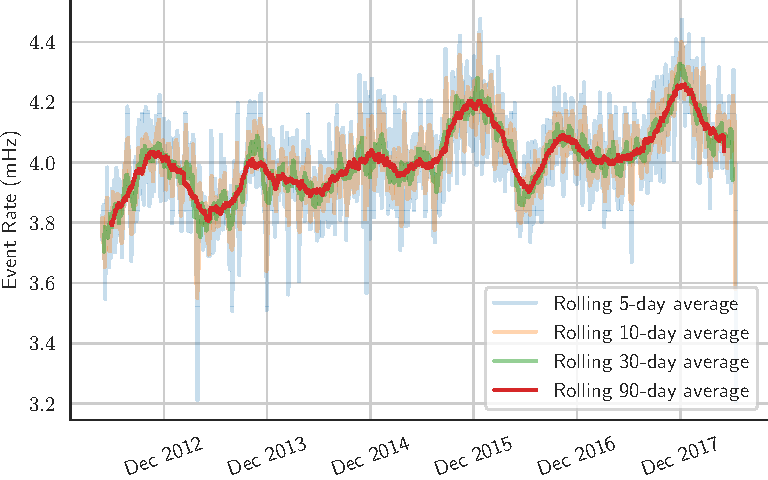
\includegraphics{llh/background_rate}
	\caption{Rolling average of final-level event rate during detector uptime.}
	\label{fig:background_rate}
\end{figure}

\subsection*{Background Spatial PDF}

The spatial distribution of the background can be neatly factorised into two distinct components, namely a zenith and an azimuth component:

\begin{equation}
	\mathcal{B}_{\textup{space}} (\theta, \phi) = \mathcal{B}_{\theta}(\theta) \times \mathcal{B}_{\phi}(\phi, \theta)
	\label{eq:b_space_local}
\end{equation}


\begin{marginfigure}
	\centering 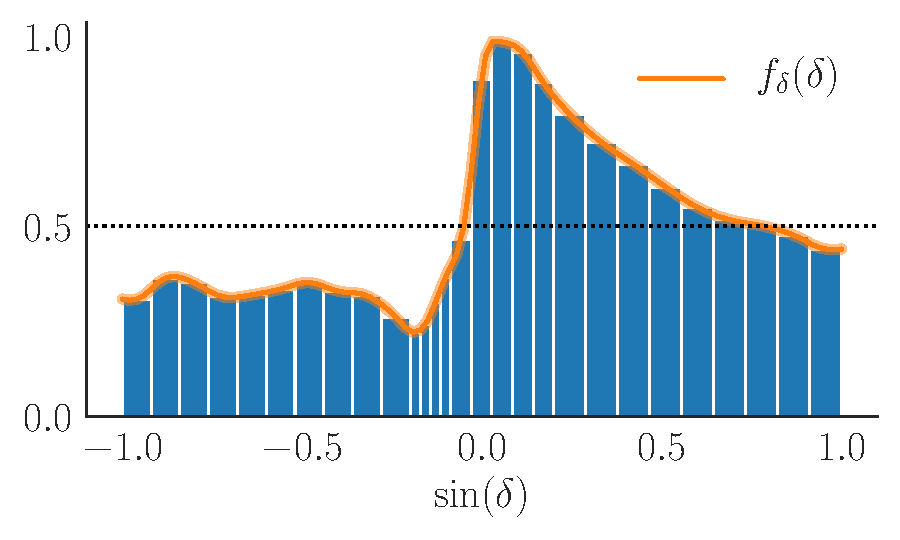
\includegraphics{llh/sindec}
	\caption{Event rate as a function of $\sin(\delta)$.}
	\label{fig:sindec}
\end{marginfigure}

Owing to IceCube's convenient location at the geographic south pole, the zenith-dependent detector response can be uniquely mapped into a declination-dependent one. With a data-driven background model, we can define a PDF $f_{\delta}(\delta)$ based on the declination-dependent event rate, as seen in Figure \ref{fig:sindec}.

\begin{equation}
	\mathcal{B}_{\delta}(\delta) = f_{\delta}(\delta)
	\label{eq:b_theta}
\end{equation}

The additional azimuthal component can be seen in Figure \ref{fig:azimuth}. The detector itself (see Chapter \ref{ch:icecube}) has 6 string axes, and these are clearly visible with elevated event rates. These variations reach up to $\sim40\%$ variations for the southern hemisphere. Additionally, the impact of \emph{ice anistropy} can be seen from an event rate deficit at and below the horizon \sidecite{2019ICRC...36..854C}, aligned with the axes of maximal charge deficit at $\sim2\pi / 3$ and $5\pi / 3$. 

\begin{marginfigure}
	\centering 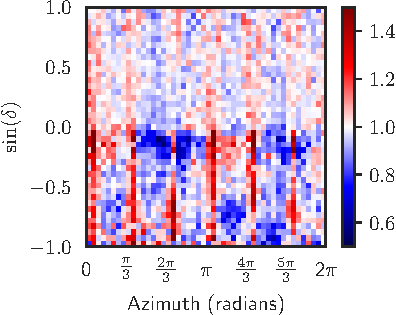
\includegraphics{llh/azimuth}
	\caption{Declination-normalised event rate as a function of azimuth.}
	\label{fig:azimuth}
\end{marginfigure}

However, string axes will all be traced out over the course of each day. Thus, for typical data periods of many years, these azimuthal variations will be averaged out. It is therefore typically assumed that \emph{any variations due to azimuthal asymmetry are negligible}.  An exception must be made for searches targeting clustering over short (sub-day) time periods, where this azimuthal asymmetry may have an impact. Beyond this, as long as the azimuth asymmetry can be neglected, we then find that the distribution in right ascension is uniform:

\begin{equation}
	\mathcal{B} (\alpha) = \frac{1}{2\pi}
	\label{eq:b_alpha}
\end{equation}

By substituting Equations \ref{eq:b_theta} and \ref{eq:b_alpha}, we can then replace Equation \ref{eq:b_space_local} with:

\begin{equation}
	\mathcal{B}_{\textup{space}} (\delta) = \frac{1}{2\pi} \times f(\delta)
	\label{eq:b_space}
\end{equation}

\subsection*{Background Energy PDF}

\begin{marginfigure}
	\centering 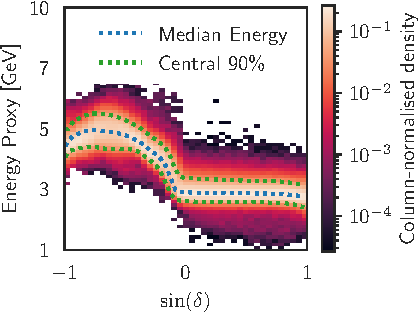
\includegraphics{llh/dec_vs_energy}
	\caption{Background energy proxy distribution, normalised in bins of $\sin(\delta)$.}
	\label{fig:dec_vs_energy}
\end{marginfigure}

Having factorised the declination dependence of events in equation \ref{eq:b_theta}, we can then consider the expected energy proxy distribution for a given spatial position. The normalised energy proxy distribution as a function of $\sin(\delta)$ is given in Figure \ref{fig:dec_vs_energy}, with the median and central 90\% ranges marked by dotted lines. It is clear that in the northern hemisphere, this distribution is essentially flat, reflecting the homogeneity of atmospheric neutrino backgrounds in this regime. However, the median energy proxy swiftly increases into the southern hemisphere, as more aggressive cuts are employed to remove the additional atmospheric muon background. The final turnover at the pole reflects the impact of the IceTop surface detector, which can be used to veto muon bundles from vertically-inclined showers.

\begin{marginfigure}
	\centering 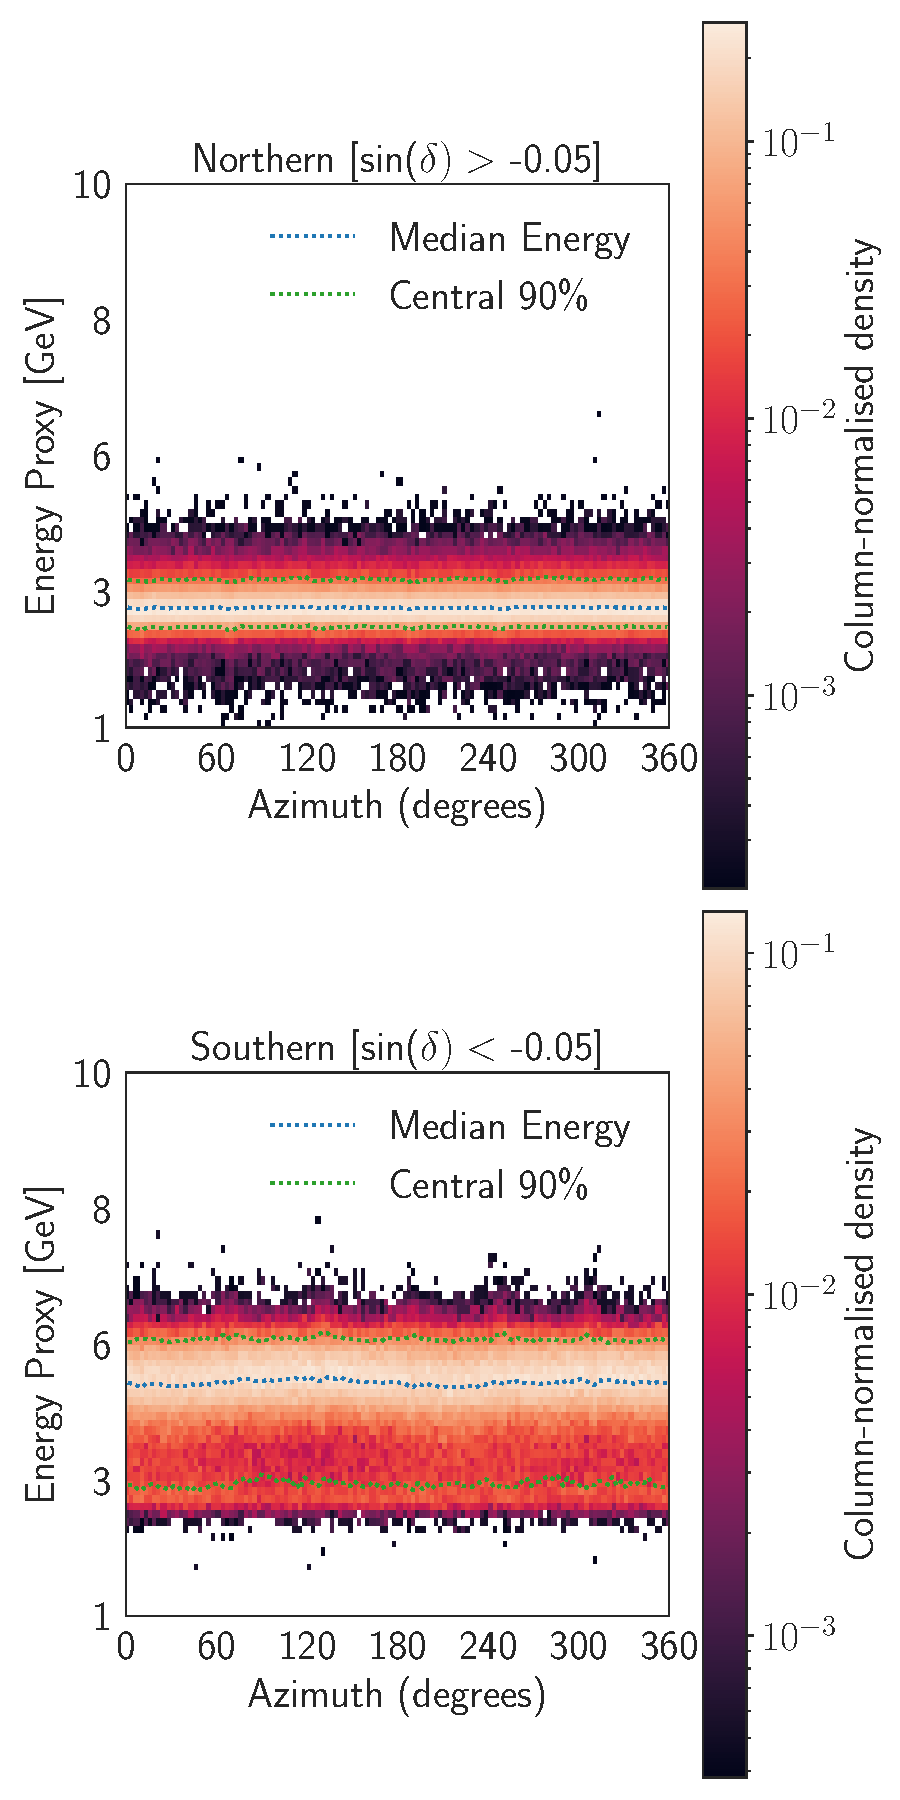
\includegraphics{llh/az_vs_energy}
	\caption{Background energy proxy distribution, normalised in bins of azimuth.}
	\label{fig:az_vs_energy}
\end{marginfigure}

In contrast to the strong declination dependence, Figure \ref{fig:az_vs_energy} shows that there is a no azimuthal dependence for events in the northern hemisphere, and negligible variation in the southern hemisphere. We can thus construct simple two-dimensional background energy PDFs using the distribution shown in Figure \ref{fig:dec_vs_energy}:

\begin{equation}
\mathcal{B}_{\textup{E}} (\delta, E_{\textup{proxy}}) = f_{\textup{E}}(E_{p}, \delta)
\label{eq:b_energy}
\end{equation}

\section{Signal Hypothesis}
\label{sec:signal}

Signal hypotheses in IceCube are a composite of the background model with a small number of additional signal-like neutrinos ($n_{s}$). It is assumed that \emph{the total number of neutrino events is essentially fixed by background}, so that N = $n_{s} + n_{b}$. In this case, we define our signal hypothesis as the normalised sum of a background PDF $\mathcal{B}$ and signal PDF $\mathcal{S}$:

\begin{equation}
\mathcal{H}= \frac{n_{s}}{N} \mathcal{S} + \frac{N - n_{s}}{N} \mathcal{B} 
\label{eq:sig_hypo_single}
\end{equation}

Much like the background, the signal PDF is a product of energy, temporal and spatial PDFs:

\begin{equation}
\mathcal{S} =  \mathcal{S}_{\textup{time}} \times  \mathcal{S}_{\textup{space}} \times\mathcal{S}_{\textup{E}}
\end{equation}

In IceCube, it is common to test hypotheses in which the the number of signal neutrinos, $n_{s}$, is a free parameter. It is also common to assume that the intrinsic signal energy PDF is an unbroken power law with some spectral index, $E^{-\gamma}$, where the spectral index $\gamma$ is an additional free parameter. 

\subsection*{Signal Time PDF}

In almost all IceCube analyses, the signal time PDF is assumed to be a uniform distribution over a fixed period of livetime. This could be for the entire duration of a dataset, corresponding to a steady neutrino source. This special case is typically referred to as a \emph{time-integrated analysis}, because it cancels out exactly the assumed background time PDF, yielding a likelihood that does not depend on time. This thesis is concerned with \emph{transient} sources, which are only active over fixed periods of time.  Transient source hypotheses require a \emph{time-dependent analysis}, in which the signal is assumed to occur over a shorter period, $T_{0}$ - $T_{1}$, than the full data-taking duration.

The uptime of the detector can be characterised by a boolean detector response function, $f_{\textup{uptime}}(t)$, that is either on (1) or off (0). The signal time PDF is then a product of the underlying source PDF and this detector response PDF. The signal PDF is normalised over the livetime, $\Delta_{T}$, between $T_{0}$ and $T_{1}$.

\begin{equation}
\Delta_{T} = \int_{T_{0}}^{T_{1}}f_{\textup{uptime}}(t) dt
\end{equation}

\begin{equation}
\mathcal{S}_{\textup{time}} (t)= 
\begin{cases}
	f_{\textup{uptime}}(t) \times \frac{1}{\Delta_{T}} & T_{0} < t < T_{1}\\
	0 & otherwise\\
\end{cases}
\end{equation}

\subsection*{Signal Spatial PDF}

The standard spatial signal PDF is typically stated to be \emph{the assumption of a circular Gaussian PSF centered on the position of a source}. For an event at $\vec{x}$ with a localisation uncertainty $\sigma$ and a source at position $\vec{d}$, we then have:

\begin{equation}
r^{2} =  (\vec{x}- \vec{d})^{2}
\end{equation}

\begin{equation}
\mathcal{S}_{\textup{space}} (\vec{x}) = \frac{1}{{2\pi\sigma^{2} }}e^{{{ - r^{2}  } \mathord{\left/ {\vphantom {{ - \left( {x - \mu } \right)^2 } {2\sigma ^2 }}} \right. \kern-\nulldelimiterspace} {2\sigma ^2 }}}
\end{equation}

In reality, even under the limit of a perfect muon track reconstruction, the unmeasurable energy-dependent kinematic angle between the incoming neutrino and outgoing muon will limit the resolution of any search. The signal PSF thus depends on the signal hypothesis, where higher-energy neutrinos are better reconstructed even for fixed $\sigma$. 

Ultimately, the performance of directional reconstructions is verified on MC events, and energy-dependent biases in uncertainty estimates are corrected in a process known as pull corrections (see Chapter \ref{ch:icecube}). So, more precisely, the signal spatial PDF is \emph{assumed to follow the distribution found in baseline MC simulations weighted with an unbroken $E^{-2}$ power law}, and further \emph{it is assumed that this distribution can be approximated by a circular Gaussian PSF with a single per-event energy-corrected uncertainty parameter}. The first assumption clearly requires that the impact of systematic uncertainties on MC simulation is negligible. The validity of these assumptions is discussed further in Chapter N, but it should be noted that neither approximation is completely valid. 

A Gaussian term for the spatial PDF also indirectly \emph{assumes that the Signal PDF does not depend on azimuth}. It is clear in the left panels of Figure \ref{fig:azimuth_mc} that azimuthal asymmetry is increasingly visible for soft spectra in the northern hemisphere, and approximately  resembles the pattern seen in Figure \ref{fig:azimuth}. However, for both the southern sky and a hard E$^{-1}$ spectrum, there is no such asymmetry. As can be clearly seen in Figure \ref{fig:mc_dec_e}, these corresponds to regimes where the signal is dominated by high-energy events. In general, \emph{the effective area at lower energies is azimuth-dependent, while at higher energies it is approximately uniform}. This is because, at lower energies, only tracks which pass close to the DOMs will be detected. In any case, as can be seen in the right-hand panels of Figure \ref{fig:azimuth_mc}, azimuth has very little discriminating power for any spectral index, and can thus be safely neglected for analysis.

\begin{figure}[!ht]
	\centering 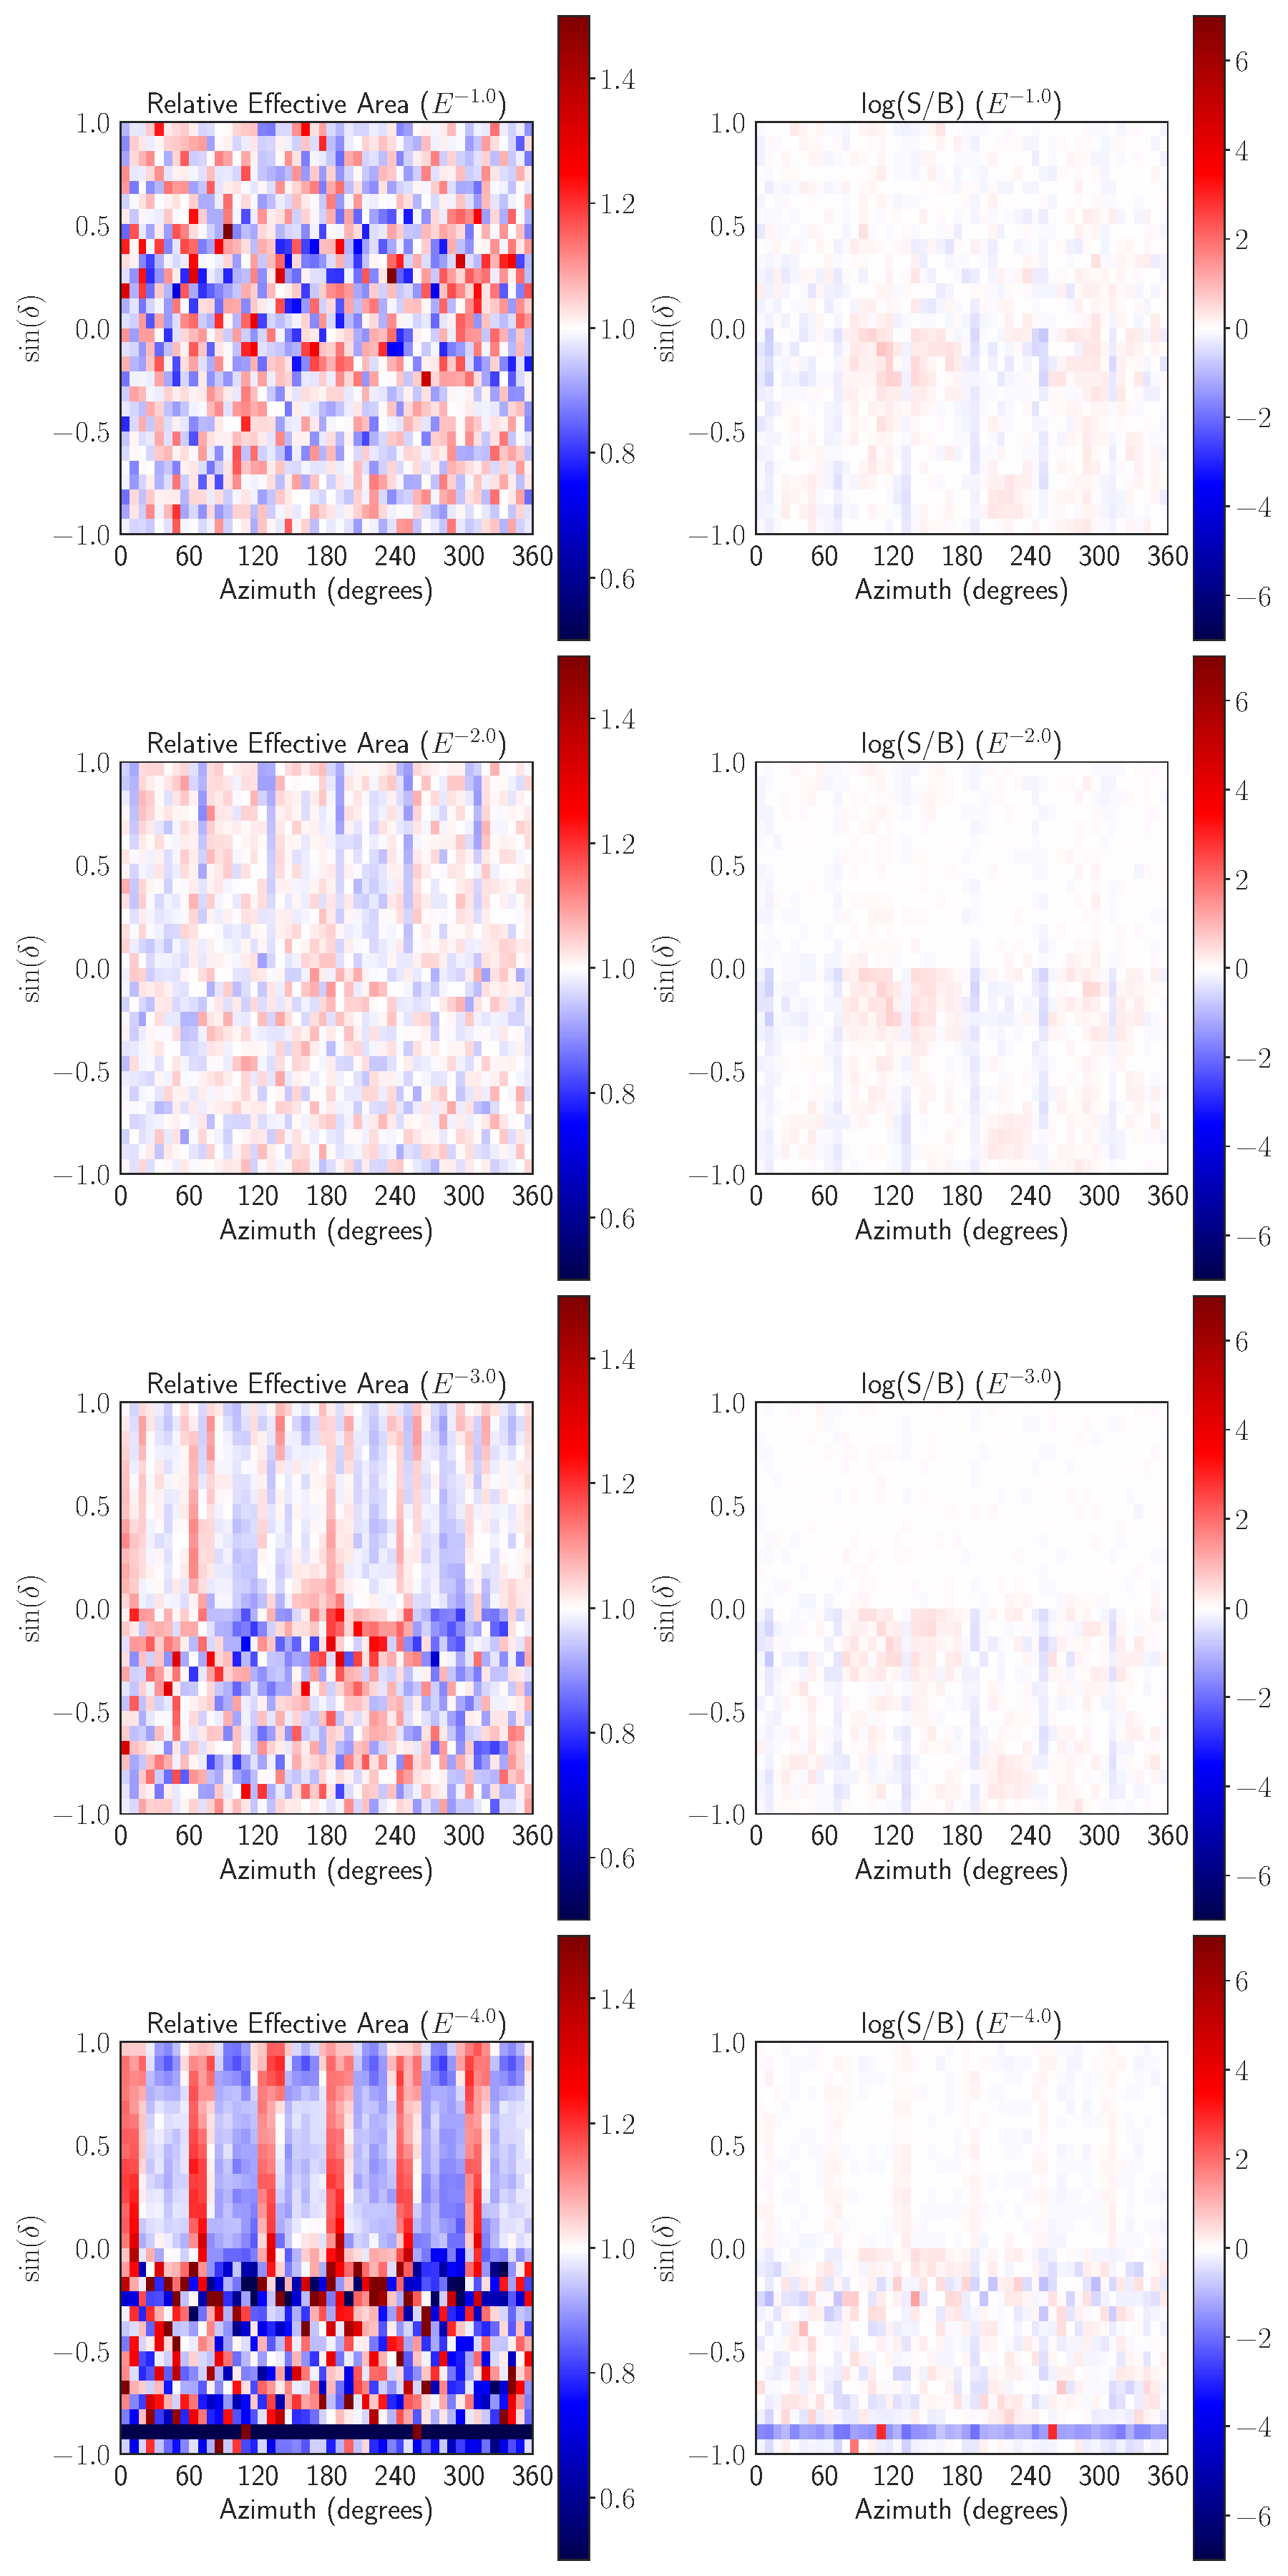
\includegraphics{llh/azimuth_mc}
	\caption{Left: Declination-normalised MC rate as a function of azimuth. Right: Ratio of declination-normalised Signal and Background PDFs.}
	\label{fig:azimuth_mc}
\end{figure}

\subsection*{Signal Energy Proxy PDF}

The energy PDF is most commonly \emph{assumed to be an unbroken power of index $\gamma$ extending over the entire energy range of sensitivity for the IceCube detector}, namely from 100 GeV to 10 PeV. This energy spectrum is then convolved with the detector response function through use of weighted MC simulation, yielding an expected distribution of energy proxy values:

\begin{equation}
\mathcal{S}_{\textup{E}} (\delta, E_{\textup{p}}, \gamma) = f_{\textup{E}}(\delta, E_{\textup{p}}, \gamma)
\label{eq:s_energy}
\end{equation}

An illustration of the expected signal distribution, derived from MC for a range of spectral indices, is illustrated in the left panels of Figure \ref{fig:mc_dec_e}. It is clear that hard spectra result in events with energies substantially above those expected in background, but for softer spectra the distribution narrows and is much more similar to that in Figure \ref{fig:dec_vs_energy}. Much of the discriminating power in IceCube comes from the identification of these high-energy neutrinos, which are unlikely to arise from atmospheric backgrounds but should arise from hard $\sim E^{-2}$ spectra expected for most astrophysical neutrino sources. 

Similar to the spatial PDF, the signal energy proxy PDF \emph{ultimately assumes that the baseline MC accurately describes the expected energy proxy distribution}. This again implicitly assumes that systematic uncertainties have a negligible impact on energy proxy distributions. 

\begin{figure}[!ht]
	\centering 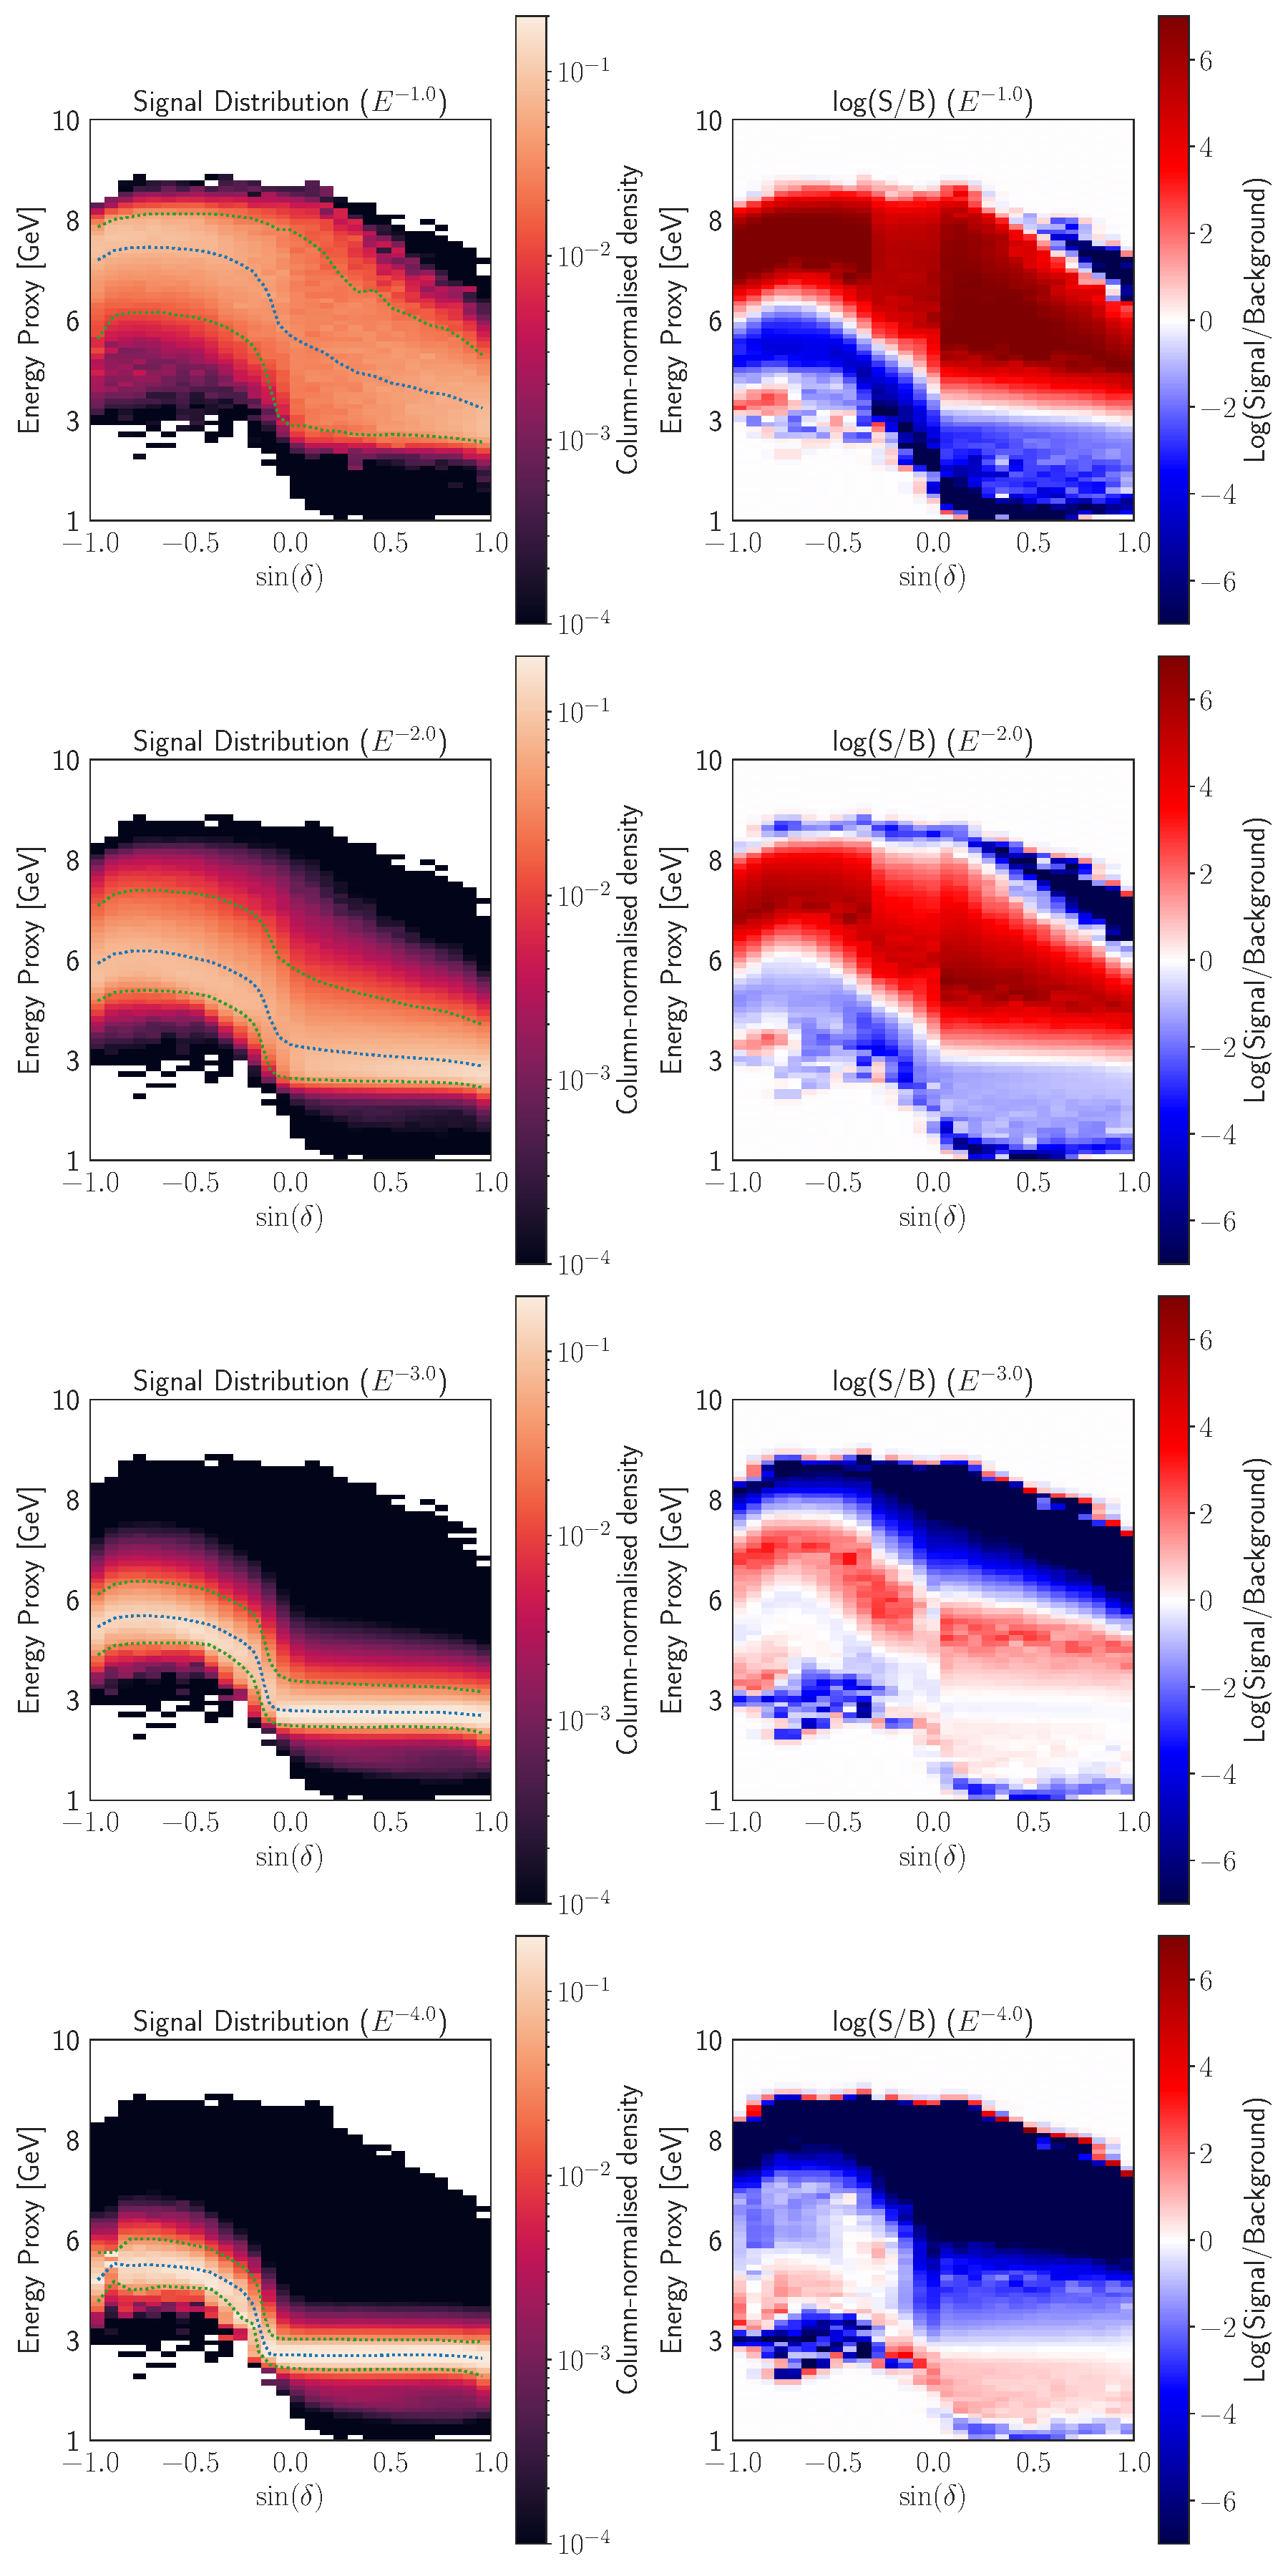
\includegraphics{llh/MC_dec_E}
	\caption{Left: Energy proxy distribution as a function of $\sin(\delta)$, for various signal hypotheses. Right: Ratio of declination-normalised Signal and Background PDFs.}
	\label{fig:mc_dec_e}
\end{figure}

\section{Likelihoods and Wilk's Theorem}

One method of quantifying agreement between a hypothesis and data is to calculate the \emph{likelihood}, $\mathcal{L}$, of observing our data given that hypothesis. Using the PDFs describing how we would expect observables to be distributed for each hypothesis, we can calculate the conditional probability, $\mathcal{L}(x | \mathcal{H})$, of observing our data $x$ given that hypothesis. The likelihood values can be used to construct a test statistic:

\begin{equation}
TS (\mathcal{H_{i}}) = 2 \log \left( \frac{\mathcal{L}(x | \mathcal{H_{i}})}{\mathcal{L}(x | \mathcal{H_{0}})} \right)
\label{eq:ts}
\end{equation}

The primary motivation for using this test statistic definition comes from the \emph{Neyman-Pearson Lemma} \sidecite{1933RSPTA.231..289N}, which states that the likelihood ratio test is the most powerful possible statistical test. 

While this TS definition can be used for a likelihood that is evaluated for discrete regions of parameter space (a \emph{Binned likelihood analysis}), it has long been customary in IceCube for the likelhood to be evaulated in a continuous event-wise fashion (an \emph{Unbinned likelihood analysis}) \sidecite{braun_ps_methods}. A likelihood is constructed, and evaluated for each jth individual event, with the overall likelihood given by the product of these N independent events:

\begin{equation}
	\mathcal{L} = \prod_{i}^{N} \mathcal{L}_{i}
\end{equation}

Ultimately this yields the standard \emph{Point Source Likelihood}:

\begin{equation}
	\mathcal{L}(n_{s}, \gamma) = \prod_{i}^{N} \left(\frac{n_{s}}{N} \mathcal{S}(\theta_{i}, \gamma) + \frac{N - n_{s}}{N} \mathcal{B}(\theta_{i})  \right)
\label{eq:ps_llh}
\end{equation}

We are thus testing a continuum of hypotheses parameterised by $n_{s}$ and $\gamma$, where both $\mathcal{S}$ and $\mathcal{B}$ depend on the event-specific observables $\theta_{j}$. We typically construct the negative log likelihood ($- \log\mathcal{L}$), and then derive best-fit parameters $\hat{n}_{s}$ and  $\hat{\gamma}$ by a process of maximum likelihood estimation. We take the combination of parameters which maximises the likelihood, and use this as our final TS value. 

\section{Pseudo-trials, P-values and trial corrections}
\label{sec:pvalues}

Given a particular TS value, we must then calculate a p-value to quantify whether or not the null hypothesis can be rejected. The most simplistic method is to perform simulated \emph{pseudo-experiments} based on the null hypothesis, to quantify how often a given outcome occurs. This method critically relies on the assumption that \emph{pseudo-experiments can be accurately simulated, and thus represent the expected distribution}. 

Much like for Section \ref{sec:background}, the null distribution can be simulated using either a data-based or MC-based model. In general, for any point source analysis, data-based methods perform well because the datasets are indeed background-dominated. Furthermore, the data can be easily randomised through use of \emph{data-scrambling}, in which the detector symmetry is exploited by randomly assigning new values of right ascension to events. Furthermore, relying on the assumption that \emph{the dataset is background-dominated at all relevant timescales}, the temporal variations of the background shown in Figure \ref{fig:background_rate} can easily be accounted for by randomly reassigning the arrival time of events to other events. These methods work principally because a point source analysis is concerned with only a tiny fraction of the data, in a narrow right ascension/declination range, and thus the broader population distribution is almost completely independent of any signal hypothesis. Alternatively using MC-based models ensures there is absolutely no contamination of the background distribution with signal, but comes at the cost of introducing a dependence on the data-MC agreement for any subsequent conclusions.

An alternative method of calculating a p-value is to exploit \emph{Wilk's Theorum} \sidecite{Wilks:1938dza}. Wilk's Theorum states that the log likelihood ratio for an ensemble of datasets will be distributed according to a $\chi^{2}$ distribution, with degrees of freedom equal to the number of independent parameters. Thus, for a hypothesis depending on a known number of independent parameters, we can analytically convert any TS value to a \emph{p-value}. There are, however, caveats to Wilk's Theorum. The full formulation only applies in the limit of large samples, and in the absence of bounds on fit parameters. In IceCube this condition is usually satisfied, but there are exceptions particularly for searches on short-timescales relevant for GRB or FRB searches, where the data transitions from a background-dominated regime to a background-free one.

For most cases, including all analysis for this thesis, a hybrid approach is used. A large number of pseudotrials are generated, providing an ensemble of TS values. A $\chi^{2}$ distribution is then fit to this dataset, with the degrees of freedom and normalisation being free parameters. This fitted distribution can then be used to extrapolate from the experimental distribution (typically several hundred thousand) to even smaller p-values, such as for the 5$\sigma$ TS value which would otherwise require several million trials.

\begin{marginfigure}
	\centering 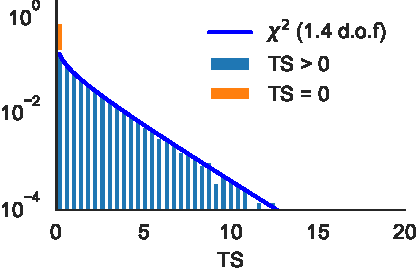
\includegraphics{llh/bkg_ts}
	\caption{Background TS distribution for the standard Point Source Likelihood (Equation \ref{eq:ps_llh}).}
	\label{fig:bkg_ts}
\end{marginfigure}

\begin{marginfigure}
	\centering 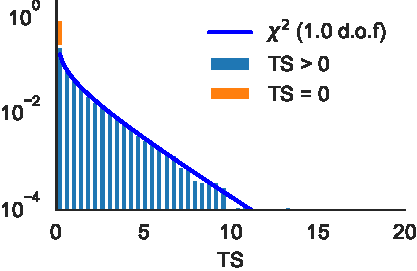
\includegraphics{llh/bkg_spatial_ts}
	\caption{Background TS distribution for a Point Source Likelihood without an energy term.}
	\label{fig:bkg_spatial_ts}
\end{marginfigure}

An example distribution, for a source at the horizon, is illustrated in Figure \ref{fig:bkg_ts}. It is well-fit by the $\chi^{2}$ distribution, with $\sim1.4$ degrees of freedom. Though this may appear to be unphysical, it illustrates the fact that the likelihood outlined in Equation \ref{eq:ps_llh} does not have two independent fit parameters. Rather, given that PS analyses search primarily for an excess of high-energy neutrinos, $n_{s}$ and $\gamma$ are in fact degenerate to a large degree. From the perspective of a likelihood analysis, a single high-energy neutrino on top of an abundant low-energy background does not appear very different to a single high-energy neutrino with a handful of lower-energy neutrinos against an abundant low-energy background. As can be seen in Figure \ref{fig:bkg_spatial_ts}, for a Point Source Likelihood without energy terms, the TS distribution is well fit by a $\chi^{2}$ distribution with exactly 1 degree of freedom, as expected for a likelihood that depends only on $n_{s}$.

For a single hypothesis, the procedure would then be complete. However, it is common that multiple hypotheses are tested at once, for example in this thesis with multiple catalogues (see Chapter \ref{ch:results}). Given that each independent test has a probability to randomly produce an overfluctuation, smaller p-values become increasingly likely as more tests are added. To counteract the multiple hypothesis problem, known as the \emph{look-elsewhere effect}, a correction must be introduced, known as a \emph{trial factor}. The trial factor quantifies the number of independent tests that have been performed, and thus quantifies how likely it is to find a small p-value. If the smallest pre-trial p-value is $p_{\textup{pre-trial}} $, then for N independent trials we find:

\begin{equation}
p_{\textup{post-trial}} = 1 - \left( 1 - p_{\textup{pre-trial}} \right)^{N}
\label{eq:trial_correction}
\end{equation}

Defining what constitutes an independent trial can be difficult. It is a common misconception that the trial factor is particularly important for cases when two hypotheses are similar. In the limit that two hypotheses are so similar as to be essentially identical, there would be no need for a trial correction at all, since the test statistic for each would be identical. The trial factor should correct the degree to which hypotheses are capable of giving multiple independent TS values. Distinct catalogues which do not share sources are completely independent trials, and thus N is simply the number of source lists tested. For correlated tests, such as overlapping catalogues or identical catalogues with different intrinsic source weighting, the trial factor will always be smaller than the number of tests but there is no analytic solution to the exact factor. Instead, it can in principle be derived experimentally, by performing all tests on each pseudo-trial, and considering the distribution of smallest p-values. In this thesis, the conservative approach is employed instead, by counting tests and assuming they are independent.

\section{Sensitivities, Discovery Potentials and Upper Limits}
\label{sec:sens_uls}

When developing and performing statistical analysis, we often wish to quantify how powerful a particular test is. As an extension of the background pseudo-experiments outlined in Section \ref{sec:pvalues}, we can also perform pseudo-experiments with our signal hypothesis, yielding a signal TS distribution. This distribution, and all conclusions derived from it, again introduce an assumption \emph{that the baseline MC can be used to represent signal}. 

With a signal TS distribution, we can characterise the power of our test by assessing the degree to which the signal TS distribution differs from the background one. For a given p-value threshold, as defined by the background model, we can calculate how frequently a given signal hypothesis would lead to a rejection of the null hypothesis. This yields the Type II error rate for any test.

The principle can be extended to cover multiple hypotheses. In the case of neutrino astronomy, a signal hypothesis can be defined for any number of signal neutrinos, $n_{\textup{inj}}$, that are \emph{injected} on top of the background model. Since the detection of signal neutrinos is a random process, the number of neutrinos can be simulated with a poisson process of mean $n_{\textup{exp}}$. We can thus parameterise a continuous set of signal hypotheses as a function of $n_{\textup{exp}}$, under the assumption of a given spectral model. 

\begin{marginfigure}
	\centering 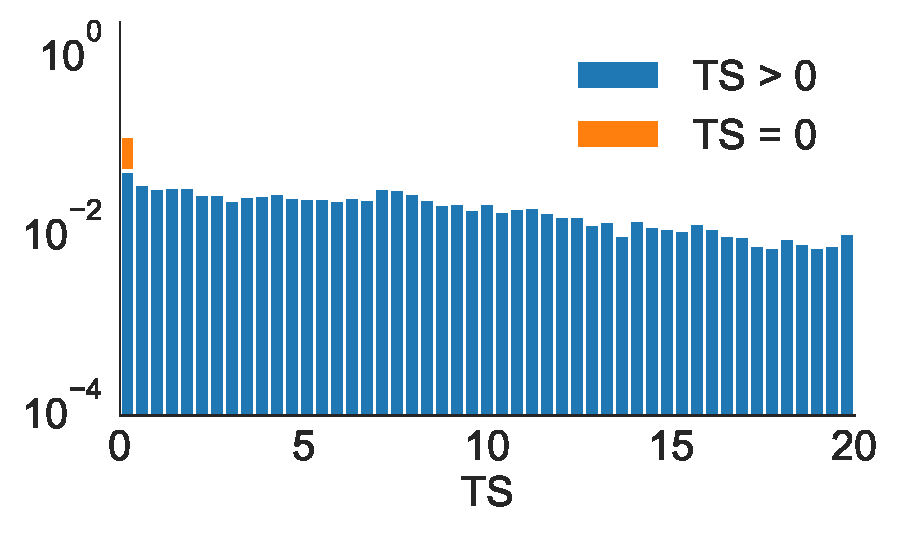
\includegraphics{llh/sig_ts}
	\caption{Signal TS distribution for the standard Point Source Likelihood (Equation \ref{eq:ps_llh}), with $\approx$ 3 injected neutrinos.}
	\label{fig:signal_ts}
\end{marginfigure}

\begin{marginfigure}
	\centering 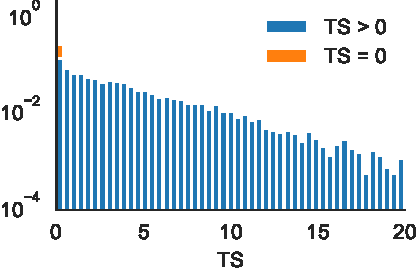
\includegraphics{llh/sig_spatial_ts}
	\caption{Signal TS distribution for the Point Source Likelihood without an energy term, with $\approx$ 3 injected neutrinos.}
	\label{fig:signal_spatial_ts}
\end{marginfigure}

An example signal TS distribution can be seen in Figure \ref{fig:signal_ts}, which covers the same time-integrated horizon source shown in Figure \ref{fig:bkg_ts} with the addition of $\approx$ 3 injected signal neutrinos. The signal TS distribution is notably shifted to higher TS values, with only 6\% of trials yielding a TS=0. The same trend is seen for Figure \ref{fig:signal_spatial_ts}, with the same number of injected signal neutrinos using a spatial-only likelihood.

It is often useful to quantify the rate of both Type  I and Type II errors associated with different regions of parameter space, especially those which rely on $n_{\textup{exp}}$. One example is the \emph{sensitivity} of a test, defined as the value of $n_{\textup{exp}}$ for which 90\% of the signal trials will yield a TS value greater than the background median. Here the Type I error rate is 50\%, and the Type II error rate is 10\%. 

Another common metric is the \emph{median 5$\sigma$ discovery potential}. This is the value of $n_{\textup{exp}}$ for which 50\% of the signal trials will yield a p-value exceeding the 5$\sigma$ threshold. In this case, the Type I error rate is $\approx 3 \times 10^{-7}$, while the Type II error rate is 50\%. The 5$\sigma$ discovery potential illustrates the region of signal parameter space for which a discovery could be expected. 

\begin{marginfigure}
	\centering 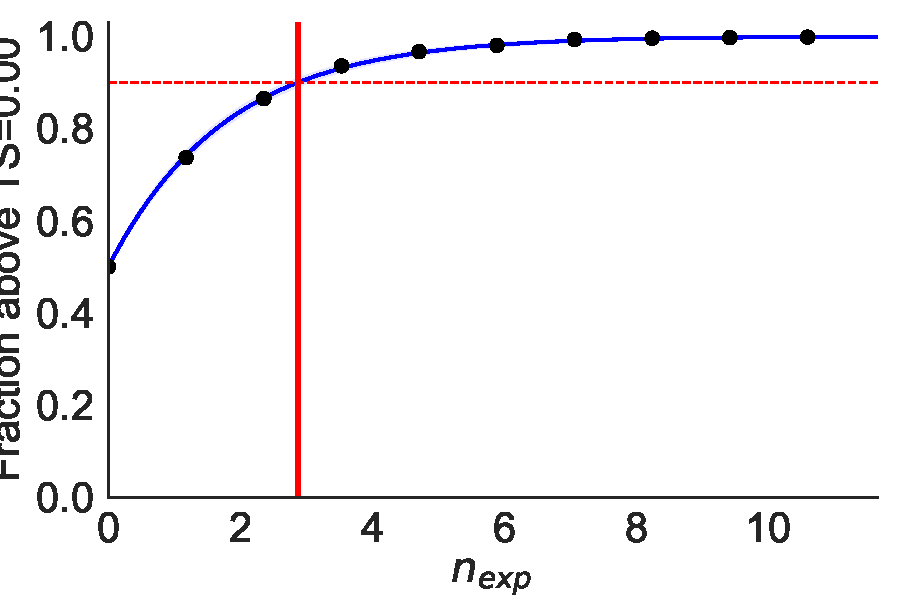
\includegraphics{llh/bkg_ts_sensitivity}
	\caption{Sensitivity for the standard Point Source Likelihood (Equation \ref{eq:ps_llh}),  using the background TS distribution from Figure \ref{fig:bkg_ts}.}
	\label{fig:sens}
\end{marginfigure}

\begin{marginfigure}
	\centering 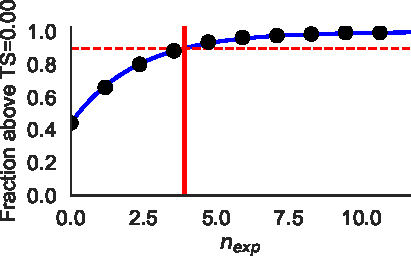
\includegraphics{llh/bkg_spatial_ts_sensitivity}
	\caption{Sensitivity for the Point Source Likelihood without an energy term, using the background TS distribution from Figure \ref{fig:bkg_spatial_ts}.}
	\label{fig:sens_spatial}
\end{marginfigure}

An example of the sensitivity is shown in Figure \ref{fig:sens}, using the background median threshold (TS=0.0)  from the distribution in Figure \ref{fig:bkg_ts}. For comparison, the spatial-only sensitivity is shown in Figure \ref{fig:sens_spatial}, relative to the corresponding background median distribution (TS=0.0) in Figure \ref{fig:bkg_spatial_ts}. While the standard Point Source Likelihood (Equation \ref{eq:ps_llh}) has a sensitivity of $\approx$ 3 signal neutrinos, the spatial-only likelihood has a sensitivity of $\approx$ 4 signal neutrinos. The latter method thus requires $\approx$ 33\% more signal to produce a likely detection, illustrating the enhanced power of the Point Source Likelihood as a statistical test. The discrepancy is even more extreme for discovery potential, with the standard method requiring $\approx$ 10 neutrinos (Figure \ref{fig:disc}) whereas the spatial-only method requires $\approx$ 18 neutrinos (Figure \ref{fig:disc_spatial}).

\begin{marginfigure}
	\centering 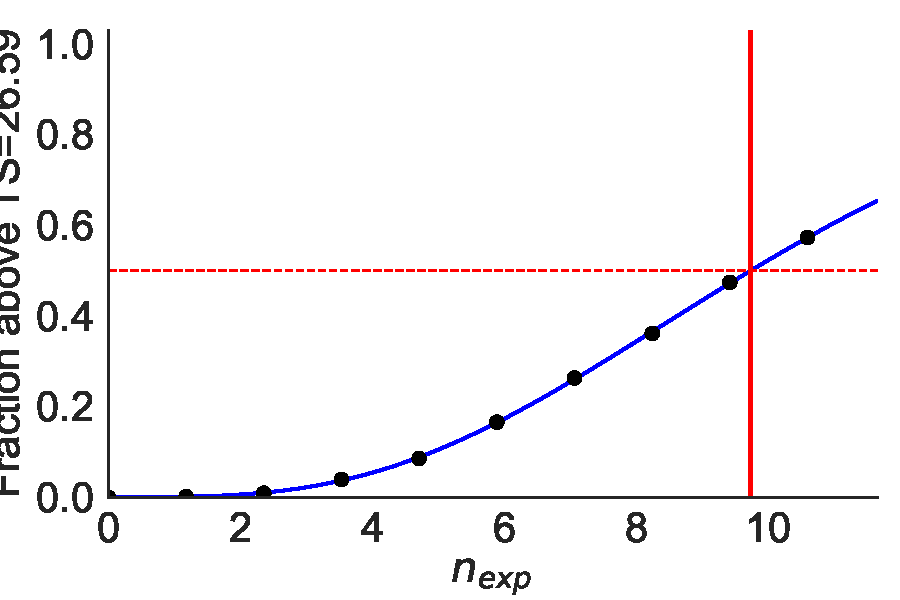
\includegraphics{llh/bkg_ts_disc}
	\caption{5$\sigma$ Discovery Potential for the standard Point Source Likelihood (Equation \ref{eq:ps_llh}), using background TS distribution from Figure \ref{fig:bkg_ts}.}
	\label{fig:disc}
\end{marginfigure}

\begin{marginfigure}
	\centering 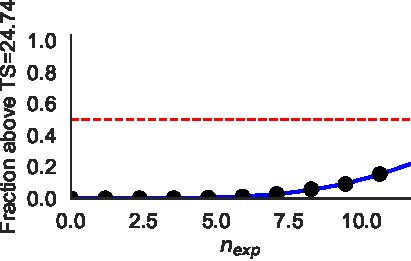
\includegraphics{llh/bkg_spatial_ts_disc}
	\caption{5$\sigma$ Discovery Potential for the Point Source Likelihood without an energy term, using background TS distribution from Figure \ref{fig:bkg_spatial_ts}.}
	\label{fig:disc_spatial}
\end{marginfigure}

These metrics allow us quantify the performance of a test without requiring knowledge of the actual outcome of the test on real data. By comparing the two cases outlined above, it clear that we should use the Point Source Likelihood with an energy term. In this way, an analysis can be designed that is \emph{blind}, and thus free from human bias. We optimise our analysis in terms of achieving the best possible sensitivity or discovery potential, and only then do we perform the test on real data. 

Once the analysis has been \emph{unblinded}, we can also recycle these pseudo-experiements to set an upper limit. Following exactly the same procedure as for sensitivity, we can derive an upper limit at some confidence level, typically 90\%, using the observed TS value and our pseudo-experients with added signal. Our upper limit is defined as the signal expectation for which 90\% of the pseudo-experiements would yield a TS greater than or equal to the value observed. By construction, for a median experimental result of the background hypothesis, the upper limit derived at 90\% confidence level is exactly equal to the sensitivity. Conventionally, in IceCube, for results which yield an underfluctuation relative to background expectations (a TS value less than the median), the sensitivity is quoted as an upper limit.

Both sensitivity and discovery potential can be used to characterise and compare the relative power of statistics tests, in terms of signal events. However, through use of the effective area,  $A_{\textup{eff}} (\delta)$, we can convert these values of $n_{\textup{exp}}$ into corresponding values of muon neutrino flux normalisation.

Under the assumption that \emph{the effective area, as derived with baseline MC, is an accurate description of the detector},  we then find for a flux of normalisation $\phi_{0}$:

\begin{equation}
n_{\textup{exp}} (\gamma) = \phi_{0} \int \mathcal{S}_{\textup{time}}(t) dt \int A_{\textup{eff}}(\delta, E_{\nu}) \times E_{\nu}^{-\gamma} dE_{\nu}
\label{eq:n_exp}
\end{equation}

The effective area as a function of declination, $A_{\textup{eff}} (\delta)$, is shown in Figure \ref{fig:effective_area}. The effective area is highest at the horizon (green lines), where it increases with neutrino energy. However, for more northern declination (yellow to red lines), the increasing impact of earth absorption suppresses neutrino detection at energies greater than 100 TeV. For the southern hemisphere, increasingly aggressive cuts to reject atmospheric muons mean that the effective area is also lower overall (blue lines), though as with the horizon there is no earth absorption of neutrinos.

\begin{figure}[!ht]
	\centering 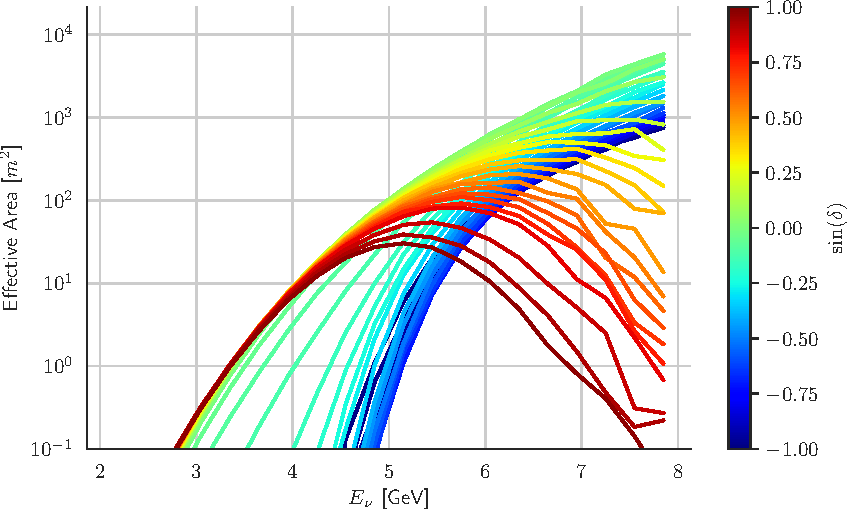
\includegraphics{llh/effective_area}
	\caption{Effective area as a function of neutrino energy and declination.}
	\label{fig:effective_area}
\end{figure}

With Equation \ref{eq:n_exp}, we can then characterise the properties of astrophysical neutrino sources for which we could expect a discovery, and conversely we can constrain these properties for a null result.

SENSITIVITY/ACROSS SKY!!!!

\section{Stacking Multiple Sources}

The simple source hypothesis outlined in Equation \ref{eq:sig_hypo_single} describes a single source, but can easily be expanded to include an ensemble of sources, known as a \emph{Stacking Analysis}. For a multi-source hypothesis, the relative contribution of each source must be accounted for.

In most cases, it is \emph{assumed that all sources share the same intrinsic neutrino spectrum}. A further assumption must be made on the fraction of catalogue flux, f$_{k}$, that each kth source will contribute. One common assumption is \emph{equal weights}, so that each of M sources contributes equally:

\begin{equation}
f_{k} = \frac{1}{M}
\end{equation}

Alternatively, another common assumption is \emph{standard candles}, where the intrinsic luminosity of each source is equal. For each kth source at lumiosity distance D$_{L,k}$

 \begin{equation}
 f_{k} = \frac{1/D_{L,k}^{2}}{\sum^{M}_{k=1}(1/D_{L,k}^{2})}
 \end{equation}

In any case, we can then calculate the expected number of signal neutrinos, n$_{k}$, for each source:

\begin{equation}
\phi_{k} = \phi_{0} \times f_{k}
\end{equation}

\begin{equation}
n_{k} (\gamma) = \phi_{0} f_{k} \int \mathcal{S}_{\textup{time, k}}(t) dt \int A_{eff}(\delta_{k}, E_{\nu}) \times E_{\nu}^{-\gamma} dE_{\nu}
\label{eq:n_k}
\end{equation}

Using Equation \ref{eq:n_k}, we can then define the fractional source weight, $w_{k}$, of each kth source:

\begin{equation}
w_{k}(\gamma)  = \frac{n_{k}(\gamma) }{\sum^{M}_{k=1} n_{k}(\gamma) } = \frac{f_{k} \int \mathcal{S}_{\textup{time, k}}(t) dt \int A_{eff}(\delta_{k}, E_{\nu}) \times E_{\nu}^{-\gamma} dE_{\nu}}{\sum^{M}_{k=1} \left( f_{k} \int \mathcal{S}_{\textup{time, k}}(t) dt \int A_{eff}(\delta_{k}, E_{\nu}) \times E_{\nu}^{-\gamma} dE_{\nu} \right)}
\end{equation}

Unlike for Equation \ref{eq:n_k}, $w_{k}$ does not ultimately depend on the flux normalisation $\phi_{0}$. For fixed spectral index, the relative contribution of different sources is independent of the number of neutrinos. Using these source weights, we can then define our normalised Signal model:

\begin{equation}
\mathcal{S}(\gamma) = \sum^{M}_{k=1} \left( w_{k}(\gamma)  \times \mathcal{S}_{k}(\gamma)  \right)
\label{eq:S_stacked}
\end{equation}

Substituting this into Equation \ref{eq:ps_llh}, we arrive at our stacked PS likelihood. Conveniently, $\mathcal{S}_{\textup{E}}(\gamma)$ does not vary by source, so can be factorised out of the sum. For steady neutrino sources, $\mathcal{S}_{\textup{time}}$ can also be factorised out, leaving only a sum over $\mathcal{S}_{\textup{space, k}}$.

\section{Combining seasons}

We can generalise the procedure even further, to account for multiple IceCube seasons. As outlined in Chapter \ref{ch:icecube}, the IceCube detector was constructed in phases, with multiple partial detector configurations each operating for roughly one year. It is conventional, as for \emph{ps tracks v003}, to include data from IC40, IC59, IC79, and IC86, where ICn refers to the number of detector strings, n,  in operation. The first year of IC86, (IC86-2011), corresponded to a different set of detector triggers, and is treated distinctly from IC86 for seasons 2012 and upward. Thus there are ultimately five distinct sets of detector operation in the ten-year point source dataset, each with a unique event selection.

These J seasons can be combined by treating them as independent datasets, and combining the likelihood for each ith neutrino in each jth season:

\begin{equation}
\mathcal{L} = \prod_{j}^{J}\prod_{i}^{N} \mathcal{L}_{i, j}
\end{equation}

The procedure outlined in Sections \ref{sec:background} and \ref{sec:signal} is followed for each dataset, yielding season-specific PDFs. The signal hypothesis can be divided in much the same way as for stacking, with a separate time PDF covering the uptime for each season ($t_{0, j} - t_1{j}$). Then, for each kth source and jth season:

\begin{equation}
\mathcal{n}_{j, k} (\gamma) = \phi_{0} \int_{t_{0, j}}^{t_{1,j}} \mathcal{S}_{\textup{time, j, k}}(t) dt \int A_{eff, j}(\delta_{k}, E_{\nu}) \times E_{\nu}^{-\gamma} dE_{\nu}
\label{eq:n_k_full}
\end{equation}

\begin{equation}
\mathcal{S}_{j}(\gamma) = \sum^{M}_{k=1} \left( w_{k, j}(\gamma)  \times \mathcal{S}_{j, k}(\gamma)  \right)
\label{eq:S_stacked_season}
\end{equation}

\begin{equation}
n_{j}(\gamma) = n_{s} \sum^{M}_{k=1} w_{k, j}(\gamma)
\label{eq:n_j}
\end{equation}

\begin{equation}
\mathcal{L}(n_{s}, \gamma) = \prod_{j}^{J} \prod_{i}^{N} \left(\frac{n_{j}}{N} \mathcal{S}_{j}(\theta_{i}, \gamma) + \frac{N - n_{j}}{N} \mathcal{B}_{j}(\theta_{i})  \right)
\label{eq:ps_llh_seasons}
\end{equation}

\section{Cluster-search algorithm}
\label{sec:cluster_algorithm}

One possible modification to the likelihood outlined above is to search for neutrino emission that is clustered in time, within a larger search window. The procedure is implemented in  \flarestack{}, and is used in this thesis for analysis of some sources. 

\begin{marginfigure}
	\centering 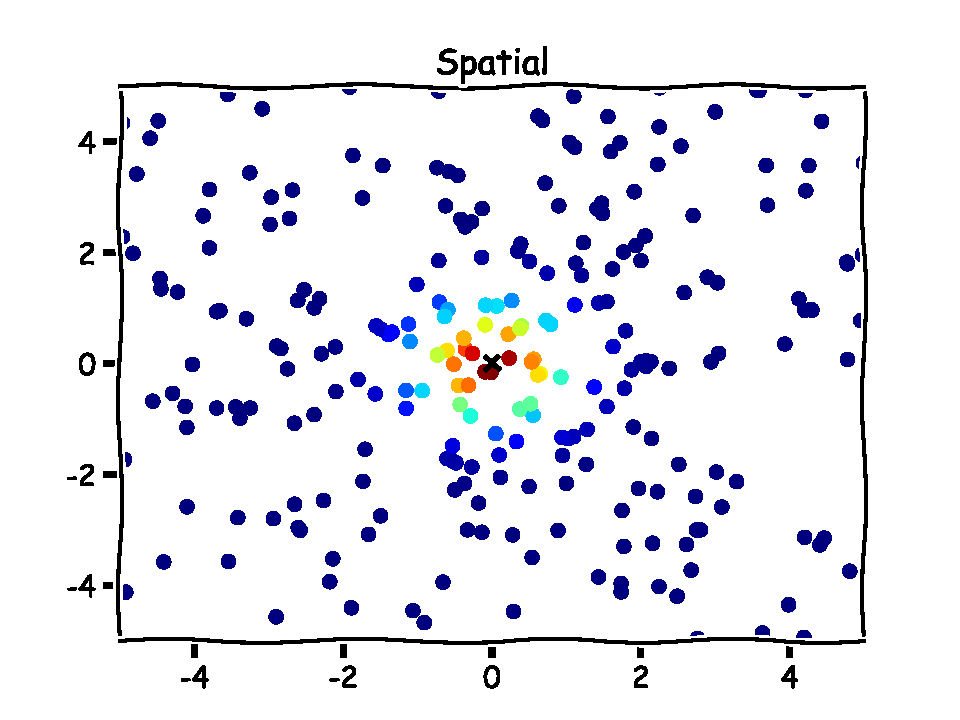
\includegraphics{llh/spatial}
	\caption{Visualisation of a spatial PDF.}
	\label{fig:spatial}
\end{marginfigure}

\begin{marginfigure}
	\centering \includegraphics{llh/energy}
	\caption{Visualisation of an energy proxy PDF.}
	\label{fig:energy}
\end{marginfigure}

Multiple box time PDFs are tested for a given source, and the one with the highest TS value is selected. Flares have both a start point, $T_{0}$, and end point, $T_{1}$, yielding two additional fit parameters. However, the likelihood landscape has discontinuities from when single neutrinos passing in/out boundary of the time PDF. Therefore, to avoid issues with minimisation by gradient descent, in  \flarestack{} the optimal flare is selected through a brute-force minimisation procedure. Though $T_{0}$ and $T_{1}$ are in principle continuous variables, the most significant possible cluster will always be one that begins and ends with the detection of a neutrino.

However, for N neutrinos in a dataset, there are $N \times (N-1)/2$ possible pairs to test. To further speed computation, a simplifying assumption is made that \emph{the most significant cluster will begin and and with signal-like neutrinos}. The $\mathcal{S}/\mathcal{B}$ ratio is calculated for all neutrinos, and only those with $\mathcal{S} > \mathcal{B}$ are considered sufficiently signal-like to test. This procedure is illustrated in Figure \ref{fig:time}.

\begin{marginfigure}
	\centering 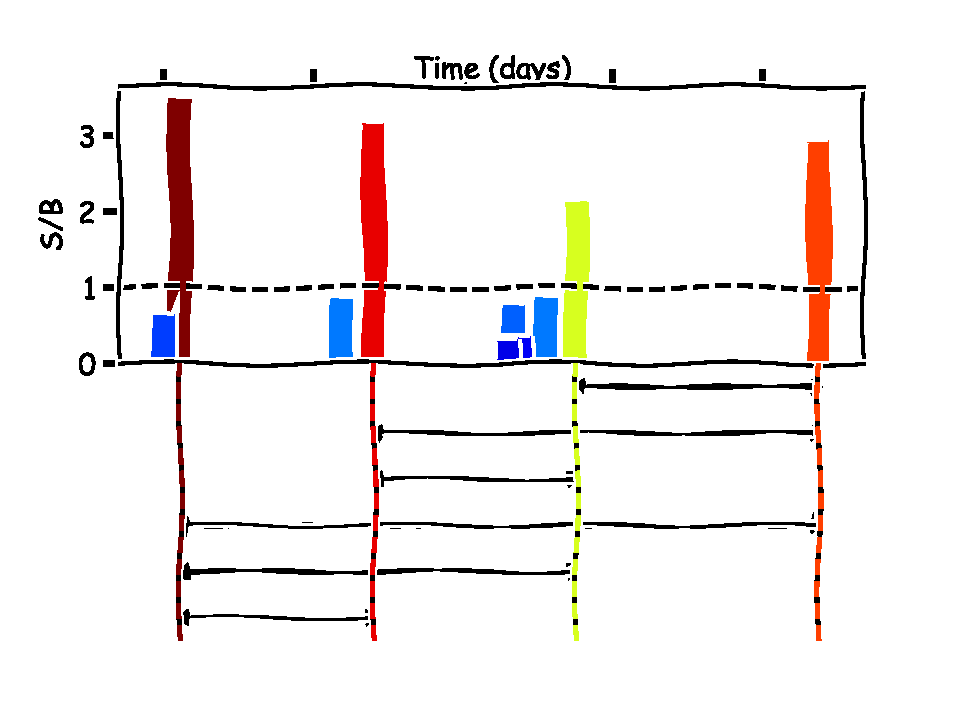
\includegraphics{llh/time}
	\caption{Visualisation of the cluster search algorithm.}
	\label{fig:time}
\end{marginfigure}

However, there is an inherent bias in such a cluster search, because there are many possible small clusters in a search window but very few possible large ones. Background fluctuations are preferentially found as small clusters. To counter this effect, a marginalisation term must be introduced to balance this bias, yielding a \emph{flare likelihood}. For a search window between $t_{0}$ and $t_{1}$, with a flare from $T_{0}$ to $T_{1}$, we find:

\begin{equation}
\Delta_{\textup{T, flare}} = \int_{T_{0}}^{T_{1}}f_{\textup{uptime}}(t) dt
\end{equation}

\begin{equation}
\Delta_{\textup{T, search}} = \int_{t_{0}}^{t_{1}}f_{\textup{uptime}}(t) dt
\end{equation}

\begin{equation}
\mathcal{L}(n_{s}, \gamma, T_{0}, T_{1}) = \prod_{i}^{N} \left(\frac{n_{s}}{N} \mathcal{S}(\theta_{i}, \gamma, T_{0}, T_{1}) + \frac{N - n_{s}}{N} \mathcal{B}(\theta_{i})  \right) \times \frac{\Delta_{\textup{T, flare}}}{\Delta_{\textup{T, search}}}
\end{equation}

An example of this cluster search, as used for the source AT2018cow (see Chapter \ref{ch:results}), demonstrates the impact on discovery potential. Given the additional degrees of freedom, there is more scope for background fluctuations, so the threshold for discovery is higher in the case that neutrino emission extends over the full search window. However, for shorter neutrino emission periods, the discovery potential is much reduced.

\begin{figure}[!ht]
	\centering 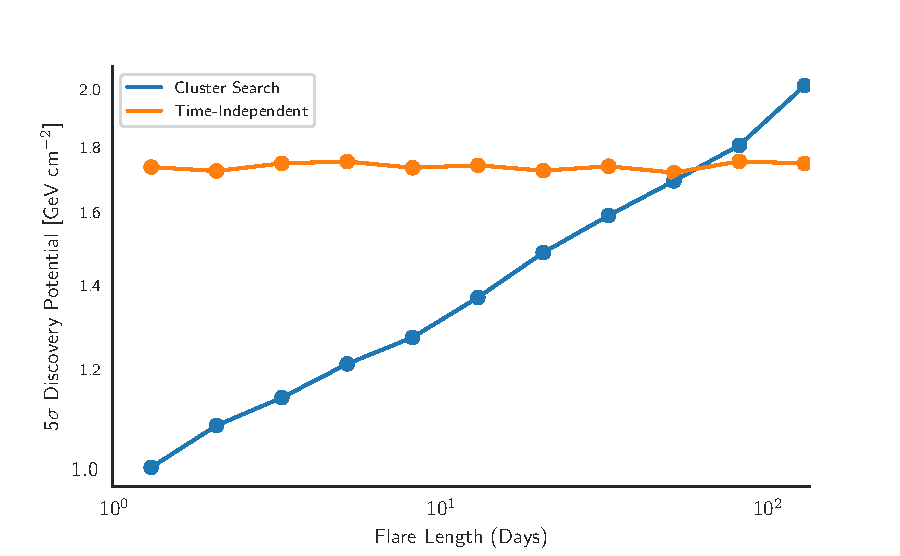
\includegraphics{llh/flare_vs_box}
	\caption{Estimated $5\sigma$ Discovery Potential for AT2018cow as a function of flare length, given in units of total fluence for an E$^{-2}$ spectrum over the 130 day search window.}
	\label{fig:DiscTime}
\end{figure}

\section{Fitting the relative source weights}
\label{sec:fit_weights}

The direct implementation of a well-defined $\mathcal{S}$ for a stacking analysis is the most powerful possible test, \emph{under the assumption that the relative distribution of the signal is known}. This condition can be satisfied when a specific model is tested that accurately predicts the relative number of signal events produced by each source in an ensemble. A prediction using multi-wavelength emission as a proxy, or expectations for a population of neutrino standard candles, are common assumptions. However, in an agnostic search for neutrino emission from a source ensemble, the uncertainty of our knowledge should be ideally implemented through priors on our expectations of neutrino emission from each source. The standard \emph{Point Source Likelihood} can be thought of as one extreme with maximum knowledge yielding $\delta$-function priors for the neutrino emission from each source. The other extreme is one of maximum ignorance, in which flat priors $n_{s, k}$ for each kth source is allowed to vary completely independently. In that case, we can replace the point-source likelihood (Equation \ref{eq:ps_llh}) with the \emph{multi-source likelihood}:

\begin{equation}
	\mathcal{L}(n_{s}, \gamma) = \prod_{j}^{N} \left(\sum_{k} \left[ \frac{n_{s, k}}{N} \mathcal{S}_{k}(\theta_{j}, \gamma) \right]+ \frac{N - \sum_{k} \left[ n_{s, k} \right] }{N} \mathcal{B}(\theta_{j})  \right)
\end{equation}

This approach is commonly referred to as \emph{fitting the weights} of each source, in contrast to the standard method of \emph{fixed source weights}. Additional flexibility comes at the expense of more independent fit parameters, and thus a higher TS threshold to achieve fixed significance. In the limit of many sources, each with sub-unity neutrino expectations, the number of degrees of freedom would exceed the number of expected signal events. It is most useful for analysing a small number of sources, in which the relative neutrino distribution is not known, but for which multiple neutrinos would be expected. This likelihood is used for some results in this thesis (see Chapter \ref{ch:results}).

\section{Flarestack in practice}
The evaulation of this likelihood is time-consuming, and the implementation of this process in  \flarestack{} makes several standard simplifications to speed calculations \sidecite{stasik_thesis}. 


The first is the recognition that the parameters which maximise the likelihood will also maximise the likelihood ratio, and thus the test statistic. Rather than evaluating two independent likelihoods, we can instead directly evaluate the test statistic:

\begin{equation}
	TS = 2 \log \left( \frac{ \mathcal{L}(\hat{n}_{s}, \hat{\gamma}) }{\mathcal{L}(n_{s} = 0)} \right)
\end{equation}
\begin{equation}
TS = 2 \log  \frac{\prod_{j}^{N} \left(\frac{n_{s}}{N} \mathcal{S}(\theta_{j}, \gamma) + \frac{N - n_{s}}{N} \mathcal{B}(\theta_{j})  \right)}{\prod_{j}^{N}\mathcal{B}(\theta_{j})}
\end{equation}

By dividing this through, we find: 

\begin{equation}
	TS =  2 \log \left(  \prod_{j}^{N} \left(\frac{n_{s}}{N} \left[\frac{\mathcal{S}(\theta_{j}, \gamma)}{\mathcal{B}(\theta_{j})} \right] + 1 - \frac{n_{s}}{N} \right) \right) 
\end{equation}
\begin{equation}
	TS = 2 \sum_{j}^{N} \log \left(\frac{n_{s}}{N} \left[ \frac{\mathcal{S}(\theta_{j}, \gamma)}{\mathcal{B}(\theta_{j}) } - 1 \right] + 1 \right) 
\label{eq:TS_reduced}
\end{equation}

Equation \ref{eq:TS_reduced}  is faster to evaluate, because it bypasses the need to calculate both signal and background energy proxy PDFs explicitly. Instead, we can precomputing the ratio $\frac{\mathcal{S}}{\mathcal{B}}$ for a variety of spectral indices, saving a per-event division calculation.

An additional simplifying assumption is that neutrinos are typically localised to a resolution of $\sim$1 degree, so events which lie many degrees from a source have a negligible probability of being signal. For events lying outside a \pm5 degree box, and those within a \pm5 degree box but with a spatial likelihood ratio less than $10^{-21}$, we make the approximation that $\mathcal{S} \approx 0$ so then $TS \approx 0$. Using the formulation in Equation \ref{eq:TS_reduced}, we see we can simply neglect to evaluate the likelihood for these events, without altering the final sum. This box cut thus removes the overwhelming majority of events from the likelihood evaluation step, yielding vast speed improvements while having a negligible impact on the fitting process.

\setchapterimage[8.5cm]{tde}
\setchapterpreamble[u]{\margintoc}
\chapter{Neutrino Source Population Fluxes}
\labch{neutrino_cosmology}
\begin{fquote}[ Kurt Vonnegut][The Design of Experiments][1935]The universe is a big place, perhaps the biggest.
\end{fquote}
%\begin{fquote}[Jocelyn Bell Burnell][Beautiful Minds][2010]The universe is very big - there's about 100,000 million galaxies in the universe, so that means an awful lot of stars.
%\end{fquote}

Often, the strictest limits on the neutrino emission of a population comes not from direct likelihood analysis, but rather from much simpler cosmological arguments. IceCube measures a diffuse astrophysical neutrino flux, setting a universal upper limit on the cumulative contribution that can come from any given population. This information can be illustrated by a \emph{Kowalski Plot}, encompassing the product of a local rate and a mean neutrino luminosity per source (see Chapter \ref{ch:sources}). 

As part of this thesis, a software framework was developed to analytically calculate neutrino emission from cosmological populations. This is integrated into the \emph{\href{https://github.com/IceCubeOpenSource/flarestack}{Flarestack}} python package, written by the author \sidecite{flarestack}.

\section{Cosmological Source Rates}

Populations of astrophysical transients are characterised by their \emph{rate} (how often they occur in the local universe), and their source evolution (how does their rate change as a function of redshift). Steady astrophysical populations are similarly characterised by a \emph{density} and \emph{density evolution}. Transient rates are typically estimated from unbiased (magnitude-limited) surveys, such as the ZTF Bright Transient Survey \sidecite{ztf_bts}. Since many astrophysical transients outlined in Chapter \ref{ch:sources} are ultimately related to stages of stellar evolution, they tend to be strongly correlated to the \emph{Star Formation Rate} (SFR), the rate at which stars are formed at a given redshift. 

The SFR can be directly inferred using multi-wavelength surveys of galaxies \sidecite{sfr_madau_14}, exploiting the characteristic spectral ratios to quantify stellar contributions in each galaxy. Alternatively, the SFR rate can be indirectly derived using observed rates of core-collapse supernovae identified in surveys \sidecite{sfr_strolger_15}. The Core-Collapse Supernova (CCSN) Rate is then directly proportional to the SFR, related by a constant of proportionality $k_{cc}$. These two CCSN rate estimates are illustrated in Figure \ref{fig:rhoz}, and broadly agree. The SFR peaks at z$\approx$1-2, and declines thereafter. It initially has a \emph{positive evolution}, i.e it increases with increasing redshift. 
\begin{marginfigure}
	\centering 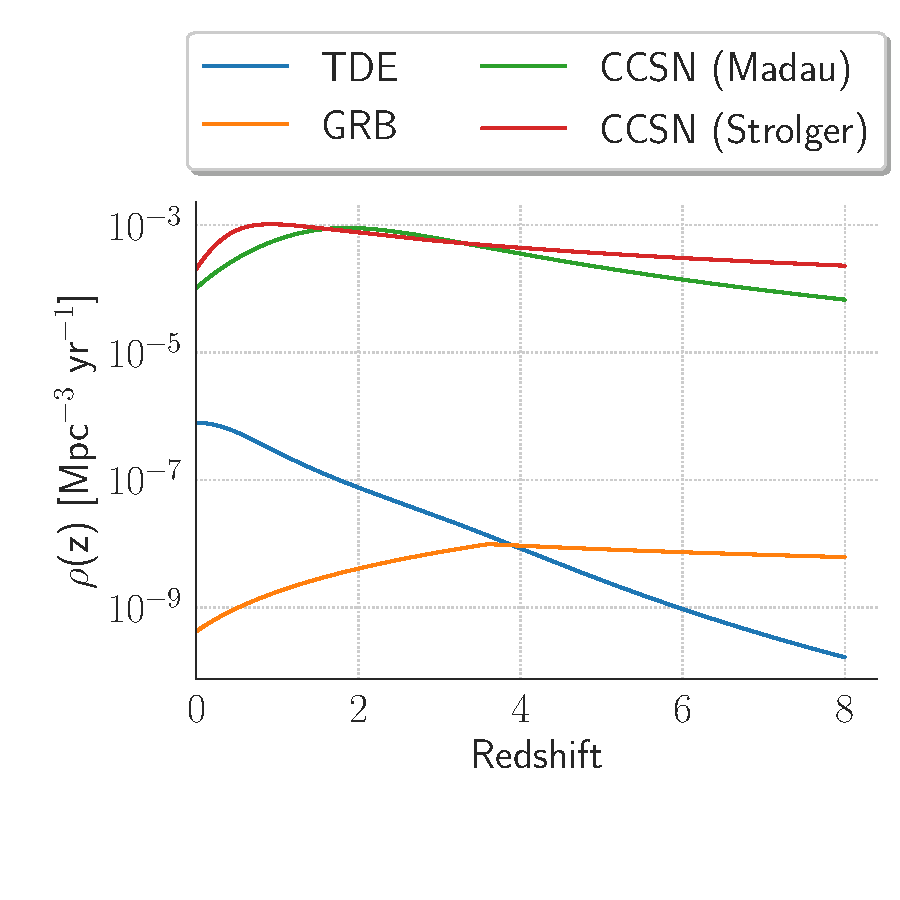
\includegraphics{nu_cosmology/rhoz}
	\caption{Various transient rate densities as a function of redshift.}
	\label{fig:rhoz}
\end{marginfigure}

An alternative driver of evolution is the density of supermassive black holes (SMBHs), which are connected with many other sources such as blazars, radio galaxies and TDEs. In contrast to the SFR, massive SMBHs are thought to be formed through mergers of smaller SMBHs. The density of massive SMBHs thus has a tendency to increase over time, so is higher in the local universe than at more distant redshifts. In contrast to the SFR, the SMBH density thus has a \emph{negative source evolution}. Of particular relevance to this thesis is the rate of TDEs, which have been proposed theoretically to follow this negative SMBH evolution  \sidecite{Sun:2015bda}, as illustrated in Figure \ref{fig:rhoz}. Caution must be taken for this rate, since TDEs are primarily detected in the local universe, so the high-z rates are broadly unconstrained observationally. 

With any chosen source rate/density and neutrino spectrum, we can calculate the corresponding \emph{cumulative neutrino flux} arising from that population \cite{Strotjohann2020Search}. For steady sources, we simply find:

\begin{equation}
\overline{\rho(z)} \equiv \frac{dN(z)}{dV_{C}}
\end{equation}

where $\overline{\rho(z)}$ is the local density per unit comoving volume. We can then integrate over the differential `redshift shell' to calculate $\overline{R(z)}$, the density per unit redshift:

\begin{equation}
\overline{R(z)} \equiv \frac{dN(z)}{dz} = \overline{\rho(z)} \times \frac{dV_{C}}{dz}
\label{eq:steady_rate}
\end{equation}

If we instead consider transient objects, additional cosmological effects start to become relevant. In the following, we denote quantities in the source frame with x', while those at Earth are given as x. It is clear that the number of particles itself must be invariant to the frame, i.e N' = N. However, there is in general a process of \emph{cosmic time dilation}, where the passage of time at the source location, t', is slowed when observed at Earth, t:

\begin{equation}
t = (1+z)t'
\label{eq:t}
\end{equation}

\begin{equation}
\frac{dt'}{dt} = \frac{1}{1+z}
\label{eq:dt}
\end{equation}

For a transient rate density $\rho (z)$ as a function of redshift, we can then calculate the rate of transients per redshift shell. The rate is given per unit time, but the impact of time dilation at higher redshifts suppresses the rate by a factor (1+z). 

\begin{equation}
\rho(z) \equiv \frac{dN(z)}{dV_{C}dt'}
\end{equation}

\begin{equation}
R(z) \equiv \frac{dN(z)}{dtdz} = \rho(z) \times \frac{dV_{C}}{dz} \times \frac{1}{1+z}
\label{eq:transient_rate}
\end{equation}

These are illustrated in Figure \ref{fig:rz}. The differential comoving volume of a redshift shell is derived using the \emph{astropy} package \sidecite{astropy_13}. We can then calculate the transient rate in the universe by integrating to high redshift:

\begin{equation}
R_{all} = \int_{0}^{\infty} R(z) dz
\end{equation}

\begin{marginfigure}
	\centering 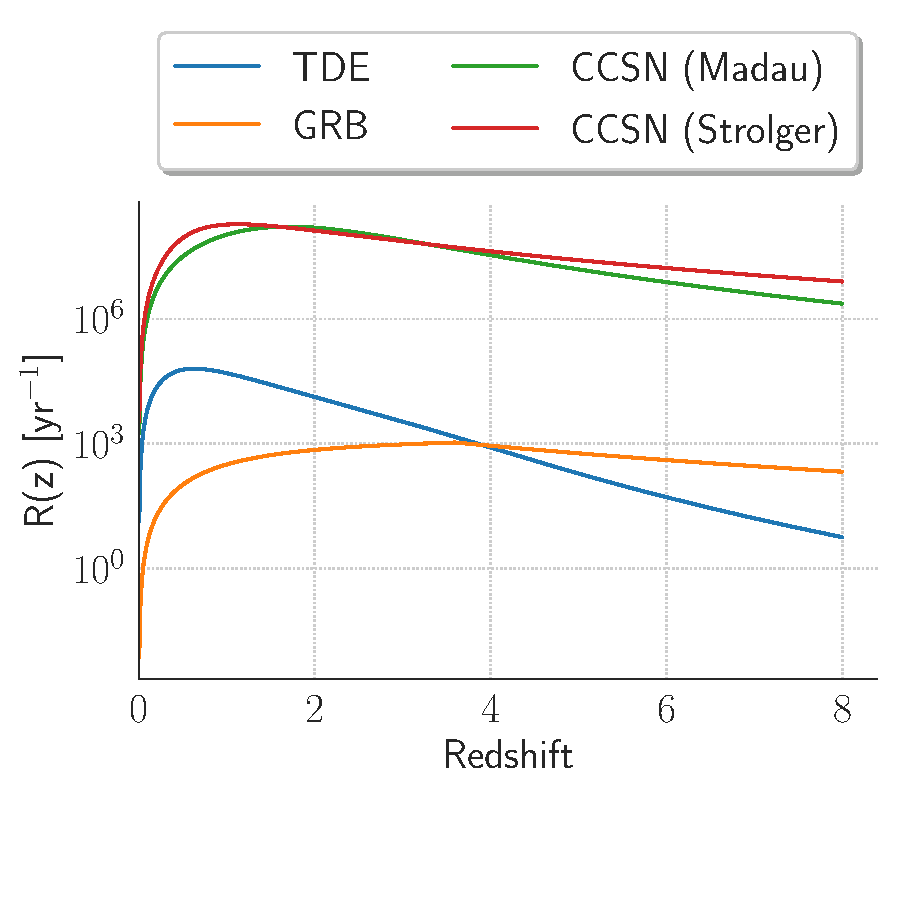
\includegraphics{nu_cosmology/rz}
	\caption{Various transient rates as a function of redshift.}
	\label{fig:rz}
\end{marginfigure}

\section{Differential flux and K-corrections}

Having  calculated the rate of sources, we must next calculate the neutrino flux produced by each individual object. We first consider the isotropic emission of a fixed number of particles, N, by a source. In that case, the particle count per unit area on Earth will ultimately depend only on the \emph{comoving distance} to that object, $D_{c}$:

\begin{equation}
\frac{dN}{dA} = \frac{N}{4 \pi D_{C}^{2}}
\label{eq:particle_per_area}
\end{equation}

If we instead wish to consider the particle flux, we must differentiate this quantity with respect to time:

\begin{equation}
\frac{dN}{dAdt} = \frac{dN}{dt} \times \frac{1}{4 \pi D_{C}^{2}}
\label{eq:particle_flux}
\end{equation}

Often, we only know the emission rate of particles in the source frame, $\frac{dN}{dt'}$, in which case we replace Equation \ref{eq:particle_flux} with:

\begin{equation}
\frac{dN}{dAdt} = \frac{1}{1+z} \times \frac{1}{4 \pi D_{C}^{2}} \times \frac{dN}{dt'}
\label{eq:alt_particle_flux}
\end{equation}

It may be more relevant to consider the luminosity of a source, where the intrinsic source luminosity is defined as:

\begin{equation}
L' \equiv \frac{d}{dt'} \left( \int E' dN \right) = \frac{d}{dt'} \left( \int E' \frac{dN}{dE'} dE' \right)
\end{equation}

However, a second cosmological effect must here be accounted for. The expansion of the universe leads to a process of \emph{redshifting}, so that E', the energy of emitted particles, is not the same as E, the energy at which the particle observed:

\begin{equation}
E = \frac{E'}{1+z}
\label{eq:redshift}
\end{equation}

\begin{equation}
\frac{dE}{dE'} = \frac{1}{1+z}
\label{eq:de}
\end{equation}

We will thus observe a redshifted energy flux, S:

\begin{equation}
S \equiv \frac{d}{dtdA} \left( \int E dN \right) = \frac{1}{1+z} \times \frac{1}{4 \pi D_{C}^{2}} \times \frac{d}{dt'} \left( \int E dN \right)
\end{equation}

\begin{equation}
S = \frac{1}{1+z} \times \frac{1}{4 \pi D_{C}^{2}} \times \frac{d}{dt'} \left( \int E \frac{dN}{dE'} dE' \right)
\end{equation}

\begin{equation}
S = \frac{1}{(1+z)^{2}} \times \frac{1}{4 \pi D_{C}^{2}} \times \frac{d}{dt'} \left( \int E' \frac{dN}{dE'} dE' \right) =  \frac{1}{(1+z)^{2}} \times \frac{L'}{4 \pi D_{C}^{2}}
\label{eq:energy_flux}
\end{equation}

Given the importance of luminosity and energy flux in astronomy, it is conventional to define a new distance measure known as \emph{luminosity distance}, $D_{L}$:

\begin{equation}
D_{L} \equiv \sqrt\frac{L'}{4 \pi S} = D_{C}(1+z)
\end{equation}

In this case, Equation \ref{eq:energy_flux} is reduced to:

\begin{equation}
S = \frac{L'}{4 \pi D_{L}^{2}}
\end{equation}

However, telescopes/detectors are only sensitive in specific energy ranges, so it is typically more important to know the flux at a given energy. This quantity, known as the \emph{differential energy flux}, is defined as:

\begin{equation}
S_{E} \equiv \frac{dS(E)}{dE} = (1+z) \times \frac{dS}{dE'}
\end{equation}

\begin{equation}
S_{E} = (1+z) \times \frac{1}{4 \pi D_{L}^{2}} \times \frac{dL'}{dE'}
\end{equation}
For convenience, we define the \emph{differential luminosity} (or \emph{specific luminosity}):

\begin{equation}
L'_{E'} \equiv  \frac{dL'}{dE'} = \frac{d}{dt'} \left( E' \frac{dN'(E')}{dE'} \right)
\end{equation}

We can then compactly write:

\begin{equation}
S_{E} = (1+z) \times \frac{L'_{E'}}{4 \pi D_{L}^{2}}
\label{eq:kcorrection}
\end{equation}

The above Equation \ref{eq:kcorrection} is the definition of a \emph{k-correction}, a widely-used formula by which the intrinsic source properties of an object can be converted to the expected differential energy flux. This is a generic definition, and is valid for both photon and neutrino fluxes. 

However, for particle detectors such as IceCube, it is instead more common to consider the differential particle flux, given by differentiating Equation \ref{eq:alt_particle_flux}. To conserve particle number despite the impact of redshifting, the observed count rate per unit energy at E, must be equal to the emission rate of particles at energy E':

\begin{equation}
dN(E) = dN'(E')
\end{equation}

\begin{equation}
\frac{dN(E)}{dE} = \frac{dN'(E')}{dE'} \times \frac{dE'}{dE} = (1+z) \times \frac{dN'(E')}{dE'}
\end{equation}

Then we see:

\begin{equation}
\frac{dN}{dAdE dt} = \frac{1}{1+z} \times \frac{1}{4 \pi D_{C}^{2}} \times \frac{dN(E)}{dEdt'}
\end{equation}

\begin{equation}
\frac{dN}{dAdEdt}= \frac{1}{4 \pi D_{C}^{2}} \times \frac{dN'(E')}{dE'dt'}
\end{equation}

For this thesis, it is only relevant to consider the special case where source spectra are power laws with some spectral index, $\gamma$:

\begin{equation}
\frac{dN'(E', t')}{dE'dt'} = \phi_{0}(t') \times \left( \frac{E'}{E_{0}}\right) ^{-\gamma}
\label{eq:def_pl}
\end{equation}

\begin{equation}
L'_{E'}(t') \equiv E' \times \frac{dN'(E', t')}{dE'dt'} = E' \times \phi(t') \times \left( \frac{E'}{E_{0}}\right) ^{-\gamma}
\label{eq:def_le}
\end{equation}

By substituting in Equation \ref{eq:redshift}, we finally reach:

\begin{equation}
\frac{dN(E', t')}{dAdEdt}= (1+z)^{2} \times \frac{1}{4 \pi D_{L}^{2}} \times \phi(t') \times \left( \frac{E'}{E_{0}}\right) ^{-\gamma}
\end{equation}

 \begin{equation}
 \frac{dN(E, t')}{dAdEdt}= (1+z)^{2 - \gamma} \times \frac{1}{4 \pi D_{L}^{2}} \times \phi(t') \times \left( \frac{E}{E_{0}}\right) ^{-\gamma}
 \label{eq:diff_particle_flux}
 \end{equation}
 
Equation \ref{eq:diff_particle_flux} is convenient for steady sources of known luminosity, where $\phi(t') = \phi_{0}$. For transients, it can be more helpful to consider the cumulative time-integrated particle flux per transient. We typically assume a constant flux for a fixed duration $\Delta_{T'} = T'_{1} - T'_{0}$:

 \begin{equation}
\phi(t')  = 
\begin{cases}
\phi_{0} & T'_{0} < t' < T'_{1}\\
0 & otherwise\\
\end{cases}
\end{equation}

\begin{equation}
\int_{0}^{\infty} \phi(t') dt' = \phi_{0} \Delta_{T'}
\end{equation}

We then find:

 \begin{equation}
 \frac{dN(E)}{dAdE} = (1+z)^{2 - \gamma} \times \frac{1}{4 \pi D_{L}^{2}}  \times \left( \frac{E}{E_{0}}\right) ^{-\gamma} \times \int \phi(t') dt 
\end{equation}

 \begin{equation}
\frac{dN(E)}{dAdE}= (1+z)^{3 - \gamma} \times \frac{\phi_{0} \Delta_{T'}}{4 \pi D_{L}^{2}} \times \left( \frac{E}{E_{0}}\right) ^{-\gamma}
\end{equation}
 
\begin{marginfigure}
	\centering \includegraphics{nu_cosmology/dnde}
	\caption{Contributed flux at earth as a function of redshift.}
	\label{fig:dnde}
\end{marginfigure}

Figure \ref{fig:dnde} shows the contributed diffuse flux at Earth as a function of redshift, assuming each transient contributes $10^{50}$ erg distributed in an $E^{-2}$ power law from 1 GeV to 10 PeV. Ultimately, the diffuse flux measured by IceCube will be the integral of this flux-per-source multiplied by the source rate in Equation \ref{eq:transient_rate}:

\begin{equation}
\frac{dN(E)}{dEdAdt} = \int_{0}^{\infty} \left[ \ (1+z)^{2 - \gamma} \times \frac{\rho(z)\phi_{0} \Delta_{T'}}{4 \pi D_{L}^{2}} \times \left( \frac{E}{E_{0}}\right) ^{-\gamma}  \right] \frac{dV_{C}}{dz} dz
\label{eq:nu_flux_tot}
\end{equation}

\begin{marginfigure}
	\centering 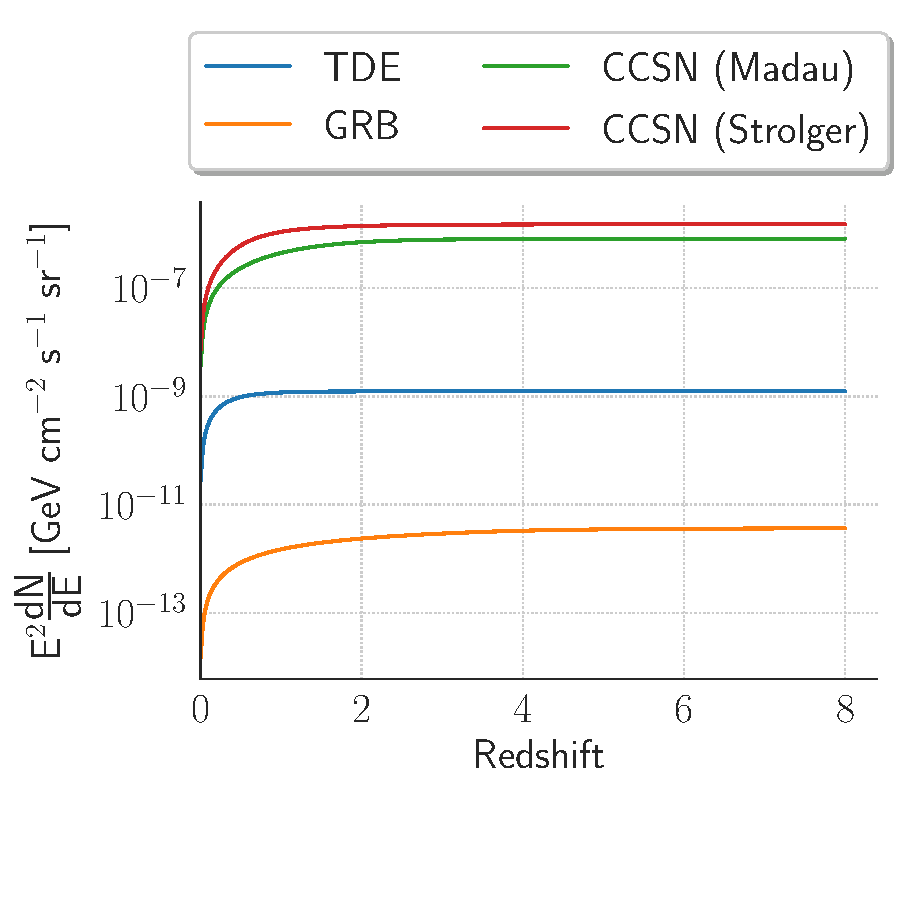
\includegraphics{nu_cosmology/diffuse_flux}
	\caption{Cumulative flux at earth as a function of redshift.}
	\label{fig:diffuse_flux}
\end{marginfigure}

These cumulative neutrino fluxes are shown in Figure \ref{fig:diffuse_flux}. For steady sources, using Equations \ref{eq:steady_rate} and \ref{eq:diff_particle_flux}, we similarly find:

\begin{equation}
\frac{dN(E)}{dEdAdt} = \int_{0}^{\infty} \left[ \ (1+z)^{2 - \gamma} \times \frac{\overline{\rho(z)}\phi_{0}}{4 \pi D_{L}^{2}} \times \left( \frac{E}{E_{0}}\right) ^{-\gamma}  \right] \frac{dV_{C}}{dz} dz
\label{eq:nu_flux_tot_steady}
\end{equation}

\section{Comparing Source Classes}

Equation \ref{eq:nu_flux_tot} reveals differences in the characteristic behaviour of different possible neutrino source populations. The impact of differing the spectral index is illustrated in Figure \ref{fig:CDF_gamma}, using the TDE rate, where softer spectral indices lead to a flux slightly more dominated by nearby sources. Given that high-z transients are already suppressed, the overall impact is relatively minor. However, as is clear in both Figure \ref{fig:dnde} and \ref{fig:CDF_rate}, the source evolution heavily impacts the relative contribution of nearby sources to the diffuse flux. A survey complete up to z=0.25 would already detect sources responsible for 60\% of all TDE neutrino emission, whereas it would contain just 20-25\% of CCSN neutrino emission. Each curve in Figure \ref{fig:CDF_rate} gives the per-neutrino probability of detecting a counterpart as a function of maximum redshift.

\begin{marginfigure}
	\centering 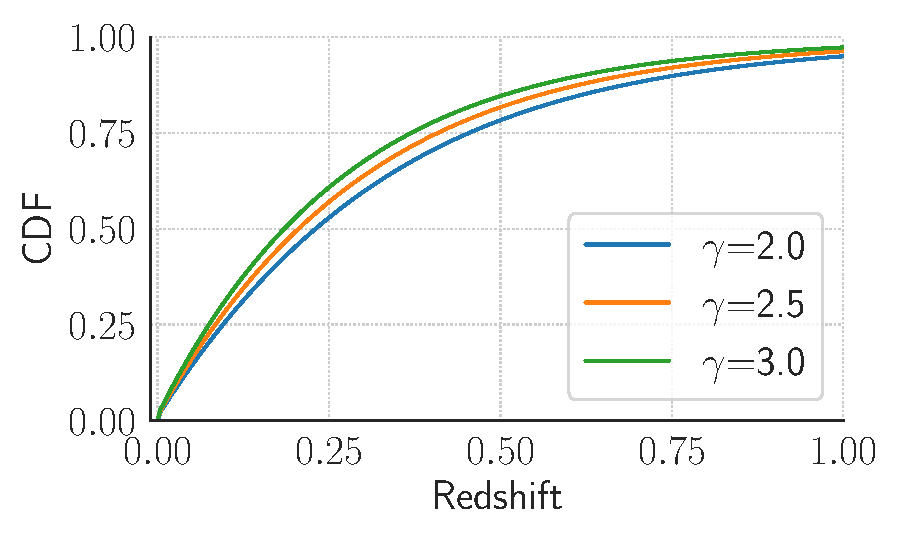
\includegraphics{nu_cosmology/flux_gamma}
	\caption{Neutrino flux CDF as a function of spectral index for TDEs.}
	\label{fig:CDF_gamma}
\end{marginfigure}


\begin{marginfigure}
	\centering 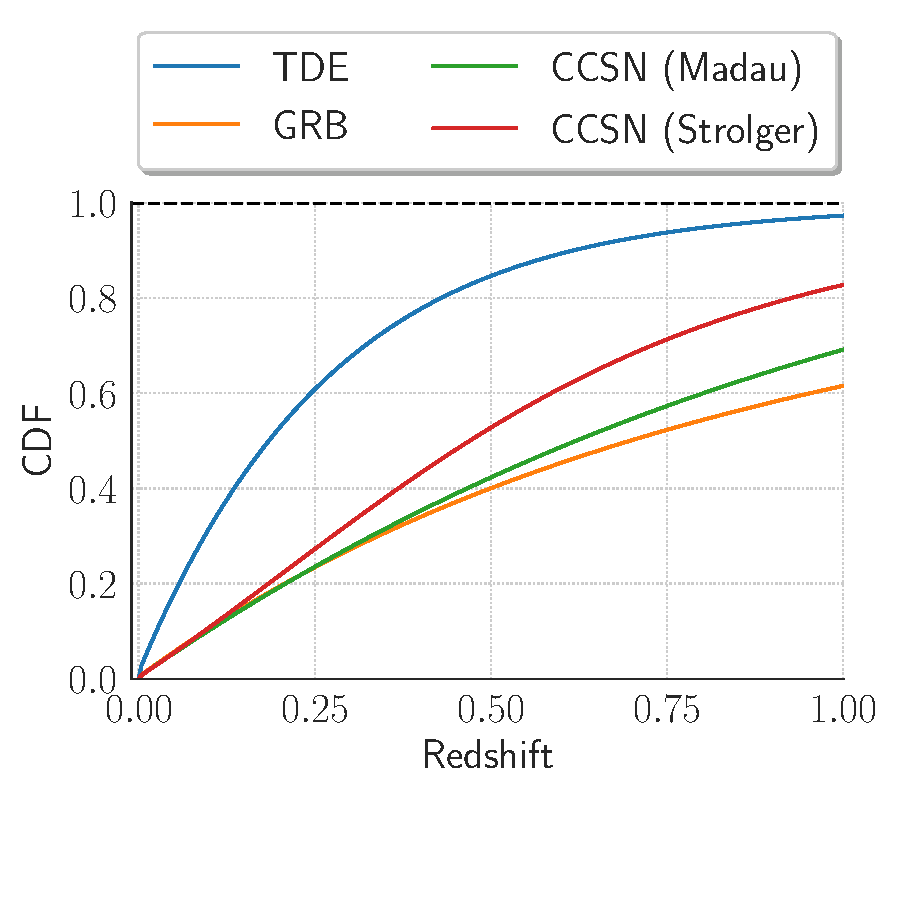
\includegraphics{nu_cosmology/diffuse_flux_rates}
	\caption{Neutrino flux CDF as a function of source evolution.}
	\label{fig:CDF_rate}
\end{marginfigure}

\begin{marginfigure}
	\centering 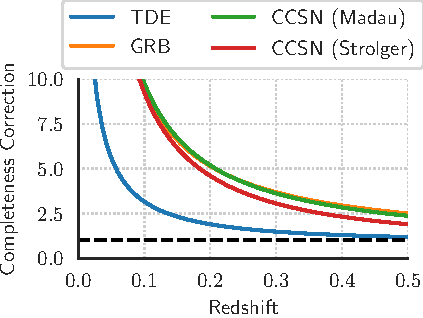
\includegraphics{nu_cosmology/diffuse_flux_completeness}
	\caption{Completeness correction factor as a function of source evolution.}
	\label{fig:completeness}
\end{marginfigure}

Figure \ref{fig:completeness} illustrates the completeness correction factor as a function of redshift. For a sample complete up to a redshift of z, multiplying the sample flux by the correction factor will yield the total population flux. Equivalently,  this factor is the number of population neutrinos that would need to be followed up before one counterpart could be identified, assuming that the follow-up instruments were sensitive up to redshift z. This Figure illustrates most starkly the challenge of optical follow-up of neutrinos, and the relative sensitivity to different source evolutions. For a TDE-like negative rate, the cumulative neutrino flux  will be overwhelmingly dominated by nearby sources, while transients that evolve with the Star Formation Rate (e.g CCSNe) have a much larger contribution from more distant sources.

To give a specific example revisited in Chapter \ref{ch:bran}, ZTF is approximately complete in identifying TDEs up to a redshift of 0.15. Per Figure \ref{fig:CDF_rate}, this volume will contain sources responsible for roughly 40\% of the population flux, so from Figure \ref{fig:completeness}, we see that we would expect to find roughly 2/5 of counterparts to TDE neutrinos. In contrast, CCSNe tend to be dimmer, and with completeness rapidly deteriorating above a redshift of z $\sim$0.05 \sidecite{ztf_bts}. Even neglecting this effect, with SFR-evolution only 12\% of neutrinos will be produced in the volume z<0.15.

To approximately quantify the impact of this effect, we can consider the general power of counting experiments probing this region. The number of signal detections, $N_{sig}$, is proportional to the fraction of flux belonging to resolvable sources, while the rate of background/chance coincidences, $N_{bkg}$, is proportional to the number of sources within this observable volume.

We consider a neutrino with typical properties for those issued as IceCube realtime alerts. We assume it has a \emph{signalness} of 50\%, i.e that it has a 50\% probability to be of astrophysical origin rather than from atmospheric backgrounds. Such alerts are typically reported with a median angular error of $\sim$1 degree. Any source class will then have a cumulative expectation of 0.5 $\times f_{\textup{tot}}$, where $f_{\textup{tot}}$ is the fraction of the total diffuse astrophysical neutrino flux contributed by that source class. 
		
We consider a number of source classes, listed in Table \ref{tab:source_properties}. We calculate their expected background rate by considering their sky rate, given as a product of their local rate, integrated to a typical telescope horizon, and multiplied by a typical telescope detection efficiency. For each source, we also multiply the appropriate search window for neutrino emission, yielding a final background density for any point on the sky. Multiplying this by the neutrino localisation area gives us the ultimate background rate per follow-up. We also consider the expected signal per search, given as the neutrino population expectation multiplied by the fraction of flux which is produced by sources accessible to telescopes. These are illustrated in Figure \ref{fig:nsig_nbkg} for a variety of source classes. Unlike other populations in Table  \ref{tab:source_properties}, GRBs are typically detected with poorly localisation, resulting in a higher background coincident rate.

\begin{table*}[]
	\centering
	\begin{tabular}{||c c c c c c c|} 
	\hline
	Source & Max & Length & Search & Detection & Local & Source \\
	Class & Redshift & &  Area & Efficiency & Rate & Evolution\\
	& [z] & [yr] & [sq. deg.] & [\%] & [Mpc$^{-3}$ yr$^{-1}$] & \\
	\hline
	TDE (Non-jetted) & 0.15 & 1.00 & 3.14 & 100.00 & 8.0$ \times10^{-7}$  & TDE \cite{Sun:2015bda}\\
	TDE (Jetted) & 0.50 & 0.50 & 3.14 & 100.00 & 3.0$ \times10^{-11}$  & TDE \cite{Sun:2015bda}\\
	SN IIP & 0.05 & 0.30 & 3.14 & 100.00 & 5.3$ \times10^{-5}$ & SFR \cite{sfr_madau_14}\\
	SN Ic & 0.05 & 0.03 & 3.14 & 100.00 & 1.8$ \times10^{-5}$  & SFR \cite{sfr_madau_14}\\
	SN IIn & 0.08 & 0.30 & 3.14 & 100.00 & 6.5$ \times10^{-6}$  & SFR \cite{sfr_madau_14}\\
	FBOT & 0.25 & 0.30 & 3.14 & 100.00 & 7.0$ \times10^{-7}$ & SFR \cite{sfr_madau_14}\\
	GRB & 1.00 & 3.2$ \times10^{-6}$ & 314.16 & 100.00 & 4.2$ \times10^{-10}$  & GRB \cite{grb_lien_14} \\
	FRB (complete) & 1.00 & 3.2$ \times10^{-10}$  & 3.14 & 100.00 & 0.072 & SFR \cite{sfr_madau_14}\\
	FRB (0.1\%) & 1.00 & 3.2$ \times10^{-10}$  & 3.14 & 0.10 & 0.072 & SFR \cite{sfr_madau_14} \\
	\hline
	\end{tabular}
	\caption{Summary of assumptions on source classes.}
	\label{tab:source_properties}
\end{table*}{}

\begin{figure}[!ht]
	\centering 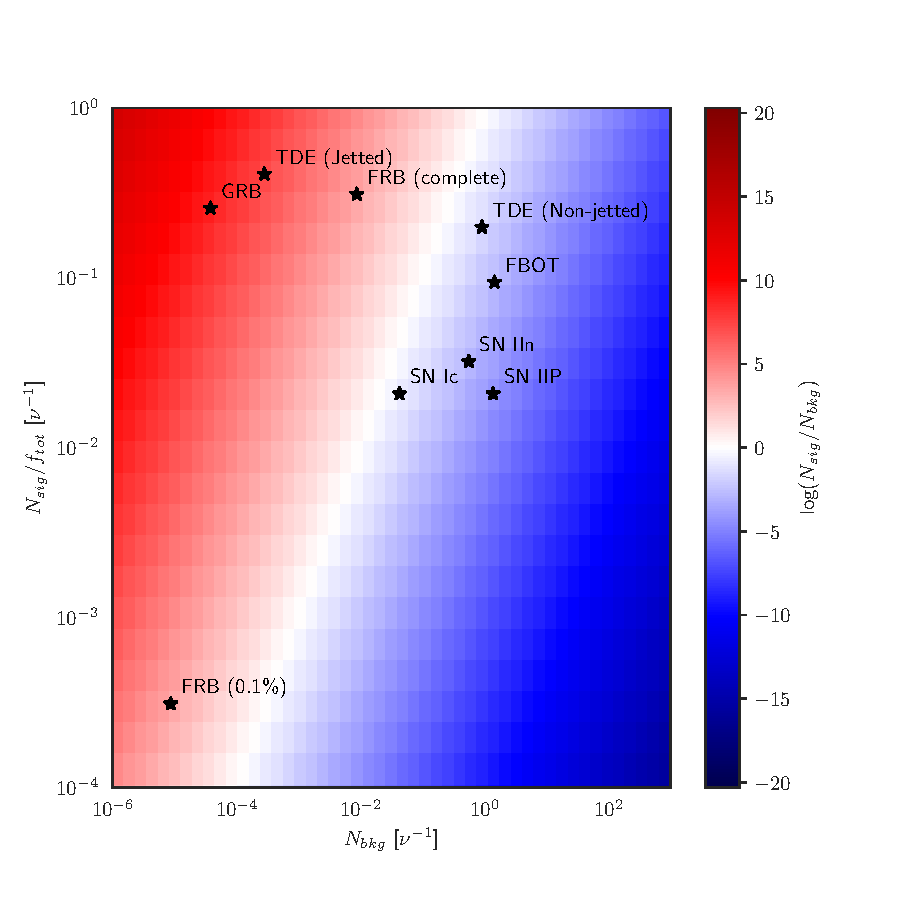
\includegraphics{nu_cosmology/nsig_nbkg}
	\caption{Per neutrino ($\nu^{-1}$) $N_{sig}$ vs $N_{bkg}$ for a variety of source classes.}
	\label{fig:nsig_nbkg}
\end{figure}

The intrinsic signal-to-noise of different source classes can be seen in Figure \ref{fig:nsig_nbkg}, with the white band indicating the transition from the red signal-dominated regions to the blue background-dominated regions. In general, the probability of observing a coincidence increases from the bottom to top, while the significance of any coincidence increases from lower right to upper left. In all cases, the y axis represents the probability of observing a coincidence. For sources with $N_{\textup{bkg}} \lesssim 0.1$, where the probability of multiple background events is negligible, the x axis corresponds to the p-value for a coincidence. Neutrino-specific properties of signalness and localisation will linearly scale all points in the x or y direction respectively, but the relative positions of populations remains unchanged. 

One particularly noteworthy class is FRBs, which should be particularly favourable owing to their extremely stringent temporal localisation. Indeed, were telescopes fully efficient at detecting these across the sky, the limits on this class would be perhaps the most stringent of all. However, at the time of the most recent IceCube analysis, just 21 FRBs were tested against an estimated rate of $\sim$3000 per sky per day, a sample for which no constraint could be placed on the FRB population \sidecite{icrc_frb}. This is a direct consequence of the detection efficiency of FRBs, which is so low that only a tiny fraction of signal is detectable. The expected signal to background ratio for FRBs is very high, and this statement is independent of detection efficiency, so any FRB-neutrino coincidence would be very strong evidence for a physical association. However, because the probability that an FRB counterpart would be detected at all is so low at present, no coincidence is likely to be found. This more realistic scenario is also illustrated in Figure \ref{fig:nsig_nbkg}, where with a more realistic assumed detection efficiency of 0.1\% FRBs illustrates the substantial contrast to other source classes.

We can further quantify how the expected significance would change with increasing numbers of follow-up campaigns for different possible source populations. In a real experiment, integer numbers of counterparts would be detected, for which we could then calculate the poisson probability of chance coincidence, the \emph{p-value} (see Chapter \ref{ch:llh}). This gives us the expected statistical significance of each Nth detection. However, the \emph{regularised lower incomplete Gamma function}, $G (y, \lambda)$, can be used to approximate a continuous poisson distribution \sidecite{incomplete_gamma}:

\begin{equation}
G (y, \lambda) = \int_{\lambda}^{\infty} \frac{t^{y-1} e^{-t}}{\Gamma (y)} dt
\label{eq:incomplete_gamma}
\end{equation}

where ${\Gamma (y)}$ is the gamma function:

\begin{equation}
\Gamma (y) = \int_{0}^{\infty} t^{y-1} e^{-t} dt
\end{equation}

Equation \ref{eq:incomplete_gamma} enables us to visualise a continuous estimate of statistical significance as a function of background rate and expected signal rate. This is shown in Figure \ref{fig:p_value}, using the same assumptions listed in Table \ref{tab:source_properties}, with the p-values converted to Gaussian $\sigma$ values. The starting x position of each curve indicates how many detections would be needed before one counterpart was detected, while the y position quantifies the statistical significance of this first signal detection given the background rate. The remainder of the curve shows how this statistical significance might be expected to evolve as a function of the number of follow-up campaigns, $N_{followup}$.

\begin{figure}[!ht]
	\centering 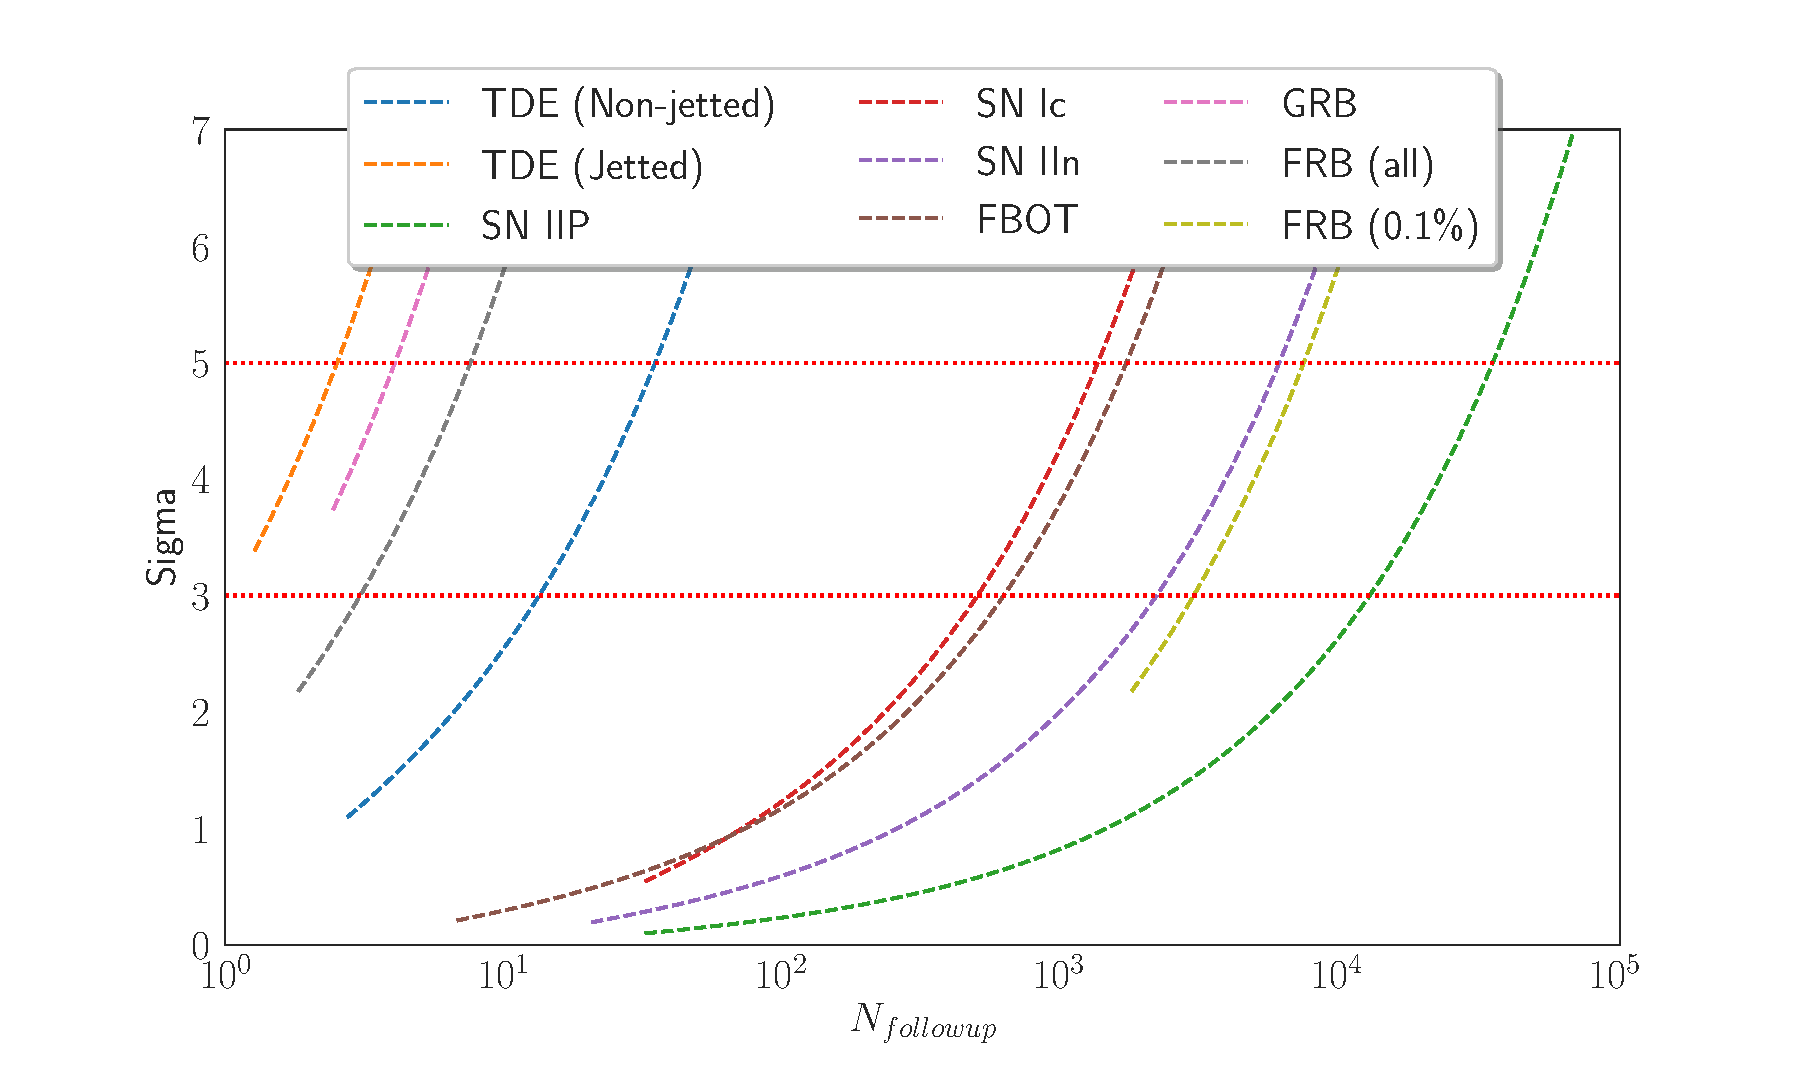
\includegraphics{nu_cosmology/p_value_nfollowup}
	\caption{Statistical significance of excess coincidence as a function of number of follow-ups.}
	\label{fig:p_value}
\end{figure}

As a lower detection efficiency will decrease the signal detection rate,  it will be represented in Figure \ref{fig:p_value} as a shift of a curve to the right,  as can be seen for the two FRB curves. However, because the background rate is also reduced proportionately, the y axis remains unaffected. In other words, with lower detection efficiency one must do more follow up campaigns to detect N coincidence, but the significance of each nth coincidence found is independent of detection efficiency.

It should be noted that the results presented in Figure \ref{fig:p_value} implicitly assume that each detected object is equally likely to be a neutrino counterpart, and are thus analogous to a so-called \emph{equal weighting} scenario as introduced in Equation \ref{eq:equal_weighting} of Chapter \ref{ch:llh}. However, rather than such a simple counting experiment, it is typical to incorporate additional information in a likelihood analysis which weight the probability for each potential counterpart. One example would be to assume neutrino emission is proportional to inverse square of luminosity distance, or to flux/fluence at a particular energy band, or correlated to a particular subclass of a population. If any such additional information is used, further background discrimination will be possible, leading to higher significance correlations for fixed $N_{followup}$. Figure \ref{fig:p_value} thus provides a lower limit on the power of any follow-up campaign targeting any source class with the properties introduced in Table \ref{tab:source_properties}. The curves do not directly depend on the observation band of a given instrument, but the individual telescope characteristics will alter the typical detection efficiency/maximum redshift. 

Though Figure \ref{fig:p_value} contains no analysis of IceCube data, it is particularly notable that the position of sources correspond closely to the relative constraints that have been placed on those classes by IceCube (see Table \ref{tab:source_limits} of Chapter \ref{ch:sources}). Those sources near the left of Figure \ref{fig:p_value} are those with the strictest existing limits, often at percent-level, while those nearer the right portion are only weakly constrained or could still produce the entire diffuse flux. The plot illustrates how well the full unbinned likelihood analysis method used by IceCube for neutrino astronomy can, to first order, be approximated by a poisson counting experiment. Those source classes on the left (TDEs, GRBs, FRBs with high detection efficiency) are those most favourable for detection with realtime follow-up programs such as the one introduced in Chapters \ref{ch:realtime} and \ref{ch:ztf}. 

\setchapterimage[8.5cm]{tde}
\setchapterpreamble[u]{\margintoc}
\chapter{Stacking Analyses with IceCube}
\labch{results}
\begin{fquote}[Oscar Wilde][Lady Windermere's Fan][1893]We are all in the gutter, but some of us are looking at the stars
\end{fquote}

A key component of this thesis is the application of the unbinned likelihood analysis method outlined in Chapter \ref{ch:llh} to specific astrophysical objects, to test for correlations indicating neutrino emission. The outcomes of these tests were then analysed in the context of diffuse neutrino flux arising from astrophysical populations, following the framework introduced in Chapter \ref{ch:neutrino_cosmology}. All results are outlined below.

All calculations were  performed using the \emph{\href{https://github.com/IceCubeOpenSource/flarestack}{Flarestack}} code, developed by the author. Some results presented were previously published in proceedings written by the author \sidecite{icrc_tde}.

\section{Tidal Disruption Events}

One novel result of this thesis is a stacking analysis of Tidal Disruption Events (TDEs) (see Chapter \ref{ch:sources}), the first such experimental search for a TDE-neutrino correlation. The details of this analysis are outlined below.

\subsection{Signal Hypothesis}

As outlined Chapter \ref{ch:sources}, theoretical modelling of neutrino emission in TDEs generally distinguishes between those with relativistic jets and those without. In recognition of this, we ultimately have two distinct hypotheses to test:

\begin{enumerate}
	\item Neutrino emission from on-axis relativistic jets
	\item Neutrino emission from other mechanisms
\end{enumerate}

The timescales predicted for neutrino emission have varied substantially. In general, neutrino emission is expected to occur close to the peak EM brightness of the flare, with durations of a few hours to $\sim$ 100 days. There are no scenarios for neutrino emission preceding disruption. 

\subsection{Catalogue Compilation}

To perform a correlation analysis, a list of sources must first be compiled. One list of TDEs is maintained by the \emph{\href{https://tde.space/}{OpenTDECatalog}} \sidecite{tde_catalog_paper}, containing relevant metadata and photometry. The database prioritises completeness by containing all objects with a possible TDE classification, even when those classifications are ambiguous \cite{tde_catalog_paper}, and will thus by construction suffer from source contamination. The database itself is maintained by volunteers, and is thus not entirely complete. For the compilation of a catalogue for this thesis, the list from the \emph{\href{https://tde.space/}{OpenTDECatalog}} was supplemented by additional objects and data from the literature.

At the time of catalogue compilation in 2018, this database contained approximately 70 objects. Of these, 3 had clear evidence of on-axis relativistic jets, while the remaining 67 did not. We further exclude those objects with peaks >100 days before the start of data-taking during the IC40 data season on 4th May 2008 (see Chapter \ref{ch:icecube}), as these objects did not overlap our neutrino dataset. We are left with 53 TDEs for correlation.

From the starting point of all TDEs, one distinct subsample was created:

\begin{itemize}
	\item \textbf{Jetted TDEs} are X-Ray-bright TDEs which launched relativistic jets pointing towards the Earth. There are three jetted TDEs, and neutrino emission is most promising from this category
\end{itemize}

These three jetted TDEs share similar properties, namely that they were all sufficiently bright to be discovered serendipitously by observations of the \textit{Swift}-BAT X-ray telescope. They each have well-sampled lightcurves, with the time of jet-launching constrained to a window of a few days. Given the consistent observational features of luminous, hard X-ray emission which rapidly fades, it is likely that all three objects are indeed jetted TDEs. The jetted TDEs were used to test Hypothesis 1.

Hypothesis 2 could then be tested with the remaining ``non-jetted'' TDEs, defined as those TDEs without on-axis relativistic jets. These non-jetted TDEs form an observationally-distinct class of objects. They may have off-axis relativistic jets, or mildly relativistic outflows, but none exhibit the characteristic hard X-ray emission associated with on-axis relativistic jets .

Beyond this, the properties of non-jetted TDEs are highly heterogeneous. They are discovered across a range of wavelengths (e.g X-ray, Optical, IR) with varying multi-wavelength coverage. There are a handful of compelling TDE candidates, often with comprehensive multi-epoch spectroscopic observations, for which alternative explanations are disfavoured. However, in the vast majority of cases, a definite classification cannot be made. To avoid contamination from misclassified objects, primarily AGN or SN, we define a clean "golden sample" consisting solely of reliably-classified TDEs:

\begin{itemize}
	\item \textbf{Golden TDEs} are strong candidates where the TDE interpretation is supported by multiple spectra
\end{itemize}

The remaining objects are then candidate TDEs, with a possible but not definitive classification. 

There is one distinct subclass of candidates, containing flares observed in dusty galaxies via IR emission \sidecite{wang_mir_tdes_2018}. One possible explanation is that the flares arise from a dust-obscured TDE, with the dust then slowly reprocessing the electromagnetic radiation from the galaxy core.  For such reprocessing, there would be a time delay between the disruption itself and the corresponding IR flare. As we expect that neutrinos should begin soon after disruption, the timescale for neutrino emission from obscured TDEs would have significant additional uncertainty. 

We thus treat these candidate \emph{obscured TDEs} separately from the other candidate TDEs:

\begin{itemize}
		\item \textbf{Obscured TDEs} are TDE candidates which occur in very dusty galaxies, and are only observed via reprocessed infra-red emission. 
	\item \textbf{Silver TDEs} are all other candidates, where a TDE interpretation is either likely or not disfavoured.
\end{itemize}

All catalogues are summarised in Table \ref{tab:stacking_cat}, with full details provided in the Appendix (Chapter \ref{ch:catalogues}).

\begin{table*}[]
	\centering
	\begin{tabular}{||c c c c |} 
		\hline
		Catalogue & Source Class & Size & Description \\ [0.5ex] 
		\hline\hline
		Jetted & Jetted TDEs &  3 & \textit{Probable TDEs with on-axis jets}\\ 
		\hline
		Golden & Non-Jetted TDEs & 13 & \textit{Probable TDEs with convincing classification}\\
		\hline
		Silver & Non-Jetted TDEs & 24 & \textit{Candidate TDEs with ambiguous classification}\\
		\hline
		Obscured & Non-Jetted TDEs & 13 & \textit{Candidate TDEs in dusty galaxies}\\[1ex] 
		\hline
	\end{tabular}
	\caption{Summary of the four TDE catalogues..}
	\label{tab:stacking_cat}
\end{table*}{}

\subsection{Search Windows}

To account for the heterogeneous datasets, an individual search window was defined for each TDE, with the aim for identifying the period of peak electromagnetic emission. For jetted/gold/silver TDE, the following criteria were used:

\begin{itemize}
	\item For TDEs in which the light curve was observed when rising, the first detection is taken as the window start.
	
	\item For TDEs without an observation during lightcurve rise, the last upper limit is taken as the window start.
	
	\item The maximum date was taken as the date on which the brightest TDE luminosity measurement was performed.
	
	\item The window extends from the defined window start to 100 days after the maximum date
	
\end{itemize}

30 days

Applying these criteria gives a tailored search window for each TDE. Obscured TDEs instead had a search window extending from 300 days before peak to 100 days after peak, to account for potential delay following neutrino emission. The search window for each source is provided in Appendix Chapter \ref{ch:catalogues}. It is the first such catalogue to contain time windows, and could also be used for stacking analyses of e.g gamma-ray emission.

\subsection{Analysis and Results}

As outlined in Chapter \ref{ch:llh}, a standard \emph{stacking analysis} requires an additional assumption on the expected relative neutrino emission of each source in a catalogue. However, these TDE catalogues are characterised by small numbers of heterogeneous sources. With a mix of observation cadences and multi-wavelength coverage, there is no obvious proxy for neutrino emission. A common standard-candle approximation, in which each source has the same intrinsic luminosity, is also not well-motivated. There is no evidence of standard-candle behaviour in EM wavelengths, so there is no reason to think it would hold for neutrino emission. We are left with no clear method to compare the relative contributions, and for this reason, an agnostic approach is instead applied. Using the method outlined in Section \ref{sec:fit_weights}, we fit the contribution of each source in the catalogue individually, requiring only that they share a common neutrino spectrum.

Following the procedure in Chapter \ref{ch:llh}, we perform an unbinned likelihood analysis to obtain results for each catalogue, with fit parameters TS, $\gamma$ and a number of signal events for each source ($n_{k}$). We also obtain a final Test Statistic (TS) value, and calculate a p-value for this TS using pseudotrials. Table \ref{tab:stacking_tests} summarises the results for each catalogue, including $n_{s} = \sum n_{k}$. The individual $n_{k}$ values are provided in the Appendix Chapter \ref{ch:catalogues}.

\begin{table}[]
	\centering
	\begin{tabular}{||c c c| c c c | c||} 
		\hline
		Catalogue & Source Class & Size & $n_{s}$  & $\gamma$ & TS & Pre-trial p-value\\
		\hline\hline
		Jetted & Jetted &  3 & 1.5& 4.0&0.8&0.40\\ 
		\hline
		Golden & Non-Jetted & 13 &3.9&2.4& 2.4&1.00\\
		\hline
		Silver & Non-Jetted & 24 &15.6&2.7&7.9 & 1.00\\
		\hline
		Obscured & Non-Jetted & 13 &29.4&2.8&14.8& 0.04\\[1ex] 
		\hline
	\end{tabular}
	\caption{Summary of results for the four TDE catalogues. For each, an independent stacking analysis was performed. The catalogues covered sources from May 2008 to October 2017, matching the IceCube data-taking period.}
	\label{tab:stacking_tests}
\end{table}{}

There was no significant correlation identified for any of the catalogues. While the Obscured TDE catalogue yielded the most significant pre-trial p-value, after trial correction using Equation \ref{eq:trial_correction} this is reduced to a value of $p_{\textup{post-trial}}$=0.15, and is thus entirely consistent with background expectations. No discovery of neutrino emission from TDEs is claimed, and \emph{we do not reject the null hypothesis that TDEs and neutrinos are uncorrelated}.

\subsection{Catalogue limits}

Being unable to reject the null hypothesis, we can instead set an upper limit on neutrino emission, by ruling out scenarios for which we would have expected to reject the null hypothesis. We follow the procedure outlined in Section \ref{sec:sens_uls} to set an upper limit, at 90\% confidence, using pseudoexperiements with simulated signal. In common with most IceCube studies, these limits are only valid \emph{under the assumption that the signal looks like the baseline IceCube MC}, and thus that \emph{the impact of all systematic effects are negligible}.

While our search results in Table \ref{tab:stacking_tests} are agnostic to the relative neutrino contribution of each source, any pseudoexperiments involving simulated signal must make an assumption regarding the intrinsic neutrino luminosity of each source. Though it remains a poor approximation for EM emission, we inject neutrinos under \emph{the assumption that each catalogue source emits the same number of neutrinos according to the same intrinsic energy spectrum}, i.e that TDEs are neutrino standard candles. The corresponding flux on Earth is thus proportional to the inverse distance squared of each source. This flux is injected uniformly across the search windows for each source, as defined in Appendix (Chapter \ref{ch:catalogues}). To conserve energy, and the flux-per-source is then inversely proportional to the length of the search window. 

The intrinsic energies are presented as \emph{isotropic-equivalent}, and thus quoted assuming that the emission is emitted isotropically. This is of particular relevance for the Jetted TDEs, for which emission is likely to be highly beamed. As the exact beaming angle is unclear, it is conventional to present such isotropic-equivalent values for comparison, with the true energy likely to be somewhat lower. All limits derived below are only valid in the case that all of these assumptions are true. Upper limits are derived for combined neutrino+anti-neutrino emission under the \emph{assumption of an unbroken neutrino power law, between 100 GeV and 10 PeV}, for a variety of spectral limits. These upper limits are shown in Figure \ref{fig:cat_upper_limit}, in units of integrated neutrino+anti-neutrino per-flavour energy for each source. 

\begin{figure}[!ht]
	\centering 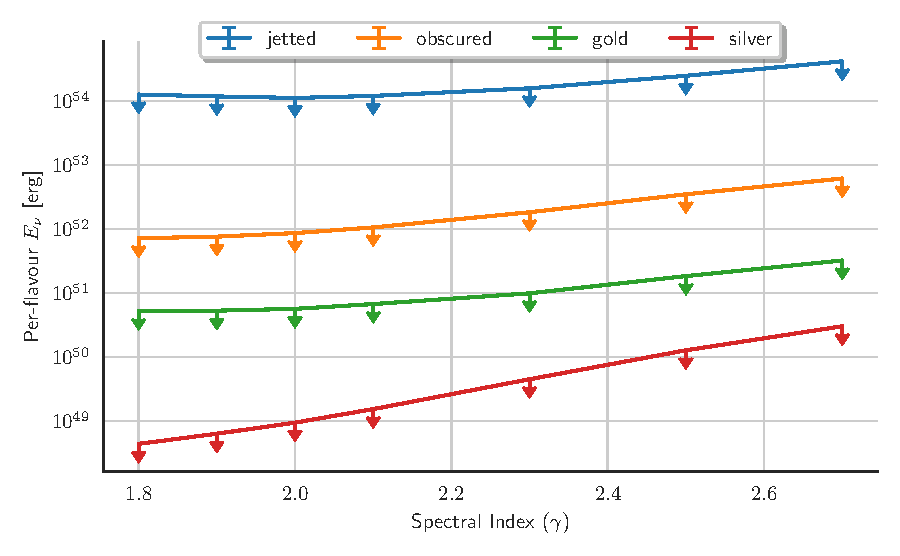
\includegraphics{results/catalogue_limits}
	\caption{Limits on the neutrino emission for each catalogue.}
	\label{fig:cat_upper_limit}
\end{figure}

\subsection{Population limits}

While the limits presented above constrain the contribution of those catalogues tested, we ultimately wish to constrain neutrino emission for the TDE population as a whole. If we \emph{assume that catalogue sources are representative of the broader population}, we can extrapolate from our per-source standard candle limits in Figure \ref{fig:cat_upper_limit} to the population flux. We seek to constrain the flux of two populations, namely jetted and non-jetted TDEs. For the latter case, we rely on the results of the golden TDE catalogue, since the extrapolation \emph{implicitly requires that the catalogues are not contaminated by misclassified objects}.

Using the most recent IceCube global fit of the astrophysical neutrino flux \sidecite{ic_global_fit_15}, with a best-fit spectrum of $E^{-2.50}$, we follow the procedure outline in Chapter \ref{ch:neutrino_cosmology}. We combine the golden TDE per-source limit shown in Figure \ref{fig:cat_upper_limit}, with a central local rate of $8 \times 10^{-7}$ Mpc$^{-3}$ year$^{-1}$ \sidecite{2018ApJ...852...72V} and a TDE source evolution \sidecite{Sun:2015bda} parameterised as:

\begin{equation}
\rho(z) \propto \left( (1 + z)^{-0.4} + \left( \frac{1 + z}{1.43} \right)^{6.4} +
\left( \frac{1 + z}{2.66} \right)^{14}
\right)^{-\frac{1}{2}}
\label{eq:tde_evolution}
\end{equation}

With this evolution, we constrain the contribution of non-jetted TDEs to be less than 25.3\% of the total. For jetted TDEs, under the assumption that they follow the same underlying source evolution in Equation \ref{eq:tde_evolution} with a central rate of $3 \times 10^{-11}$ Mpc$^{-3}$ year$^{-1}$ \cite{Sun:2015bda}, we find that they must contribute less than 1.3\% of the total.  These constraints are illustrated in Figure \ref{fig:DiffuseFlux}. 

\begin{figure}[!ht]
	\centering 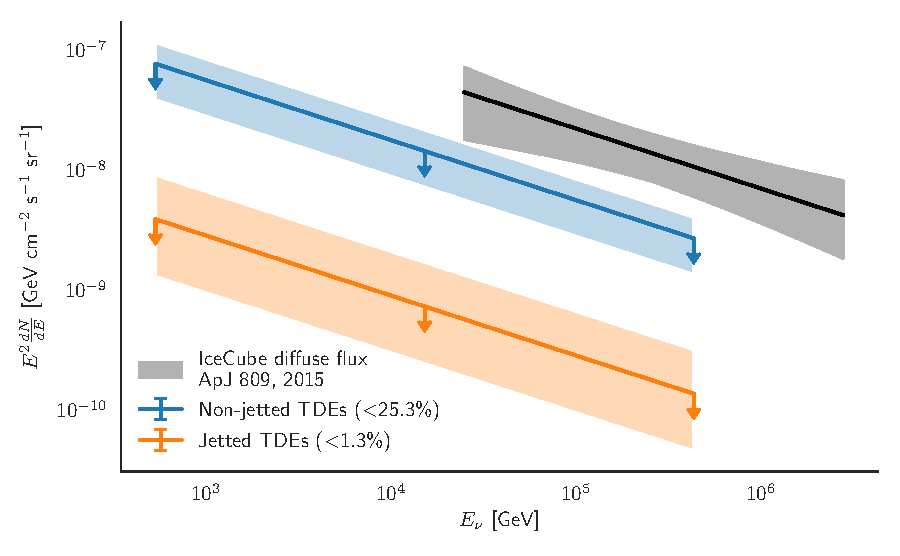
\includegraphics{results/tde_limits}
	\caption{Limits on the contribution of jetted and non-jetted TDEs to the diffuse neutrino flux.}
	\label{fig:DiffuseFlux}
\end{figure}

As the contribution from a population is directly proportional to the local population rate, the shaded bands indicate the uncertainty in our limits arising from rate estimates. For TDEs, these rates are a large source of uncertainty in neutrino flux. It will require systematic evaluation of observed TDE rates to enable more precise limits on neutrino emission. Any refined rate estimate can be used to linearly rescale these limits. Propagating through the current local rate uncertainty, we constrain non-jetted TDEs to be less than 12.7\% - 38.0\%, and jetted TDEs to be less than 0.4\% - 3.0\% of the total. With a more precise future measurement of the local TDE rate, these values can be linearly rescaled to provide more accurate limits.

Such limits also critically depend on the source evolution of TDEs as a function of redshift, but this is not strongly constrained observationally because TDEs detections are generally confined to the local universe (z $\lesssim$ 0.3). Estimates are made primarily based on theoretical predictions derived from the rate of supermassive black holes (see Chapter \ref{ch:neutrino_cosmology}) \cite{Sun:2015bda}. We can instead consider a source evolution similar to the Star Formation Rate (SFR) \sidecite{sfr_madau_14}, parameterised as:

\begin{equation}
\rho(z) \propto\frac{(1+z)^{2.7}}{1 + ((1+z)/2.9)^{5.6}}
\label{eq:sfr_evolution}
\end{equation}

With Equation \ref{eq:sfr_evolution}, we would then find limits of 108.3\% (54.2\% - 162.5\%) for non-jetted TDEs and 5.5 \% (1.8\% - 12.8\%) for jettted TDEs. These limits are shown in Figure \ref{fig:DiffuseFluxSFR}. For such a scenario, the contribution of unresolved non-jetted TDEs is so large that the measured flux itself provides a stricter constraint than the catalogue test. However, even in that extreme scenario, the contribution of jetted TDEs to the diffuse neutrino flux remains subdominant.

\begin{figure}[!ht]
	\centering 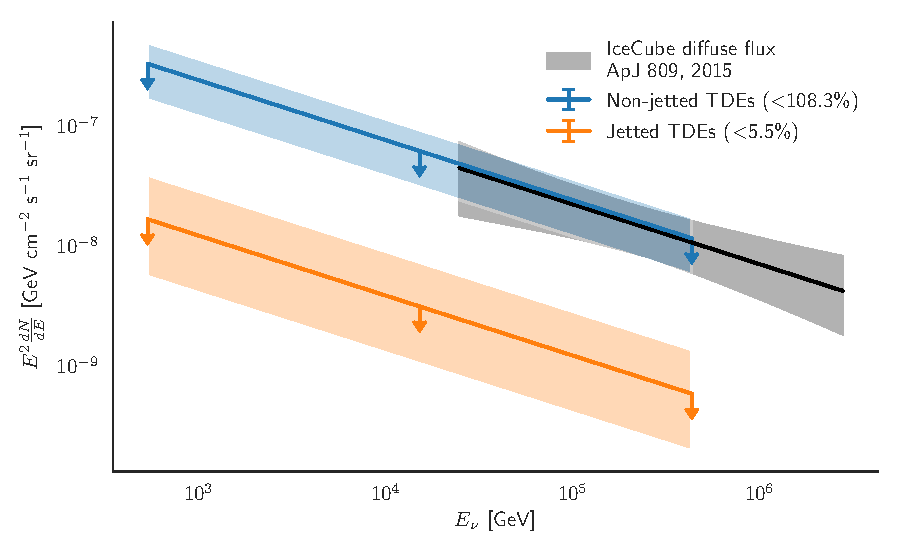
\includegraphics{results/tde_limits_sfr}
	\caption{Limits on the contribution of jetted and non-jetted TDEs to the diffuse neutrino flux, under the assumption of a source evolution proportional to the Star Formation Rate.}
	\label{fig:DiffuseFluxSFR}
\end{figure}

\subsection{Individual TDEs}

In addition to the stacking analysis, four TDEs were selected for individual analysis. Two of the three jetted TDEs, Swift J1644+57 and Swift J2058+05, were chosen due to their luminosity, as well as their position in the northern hemisphere where IceCube has the highest effective area. In addition, ASSASN-14li and  XMMSL1 J0740-85 were chosen as non-jetted TDEs which were both nearby and bright. These four TDEs were the only catalogue sources that were also detected in radio observations, typically a tracer for relativistic particle acceleration. For each of the four individual TDEs, searches were conducted for neutrino clustering in both time and space, following the procedure outlined in Section \ref{sec:cluster_algorithm}. All single-object tests are described in Table \ref{tab:single_tests}.

\begin{table*}[]
	\centering
	\begin{tabular}{||c |c c c c | c c c c| c||} 
	\hline
	Source & R.A & Dec & T$_{0}$ & T$_{1}$ & n$_{s}$ & $\gamma$ & t$_{s}$ & t$_{e}$ & TS\\
	& (deg.) & (deg.) & (MJD) & (MJD) & & & (MJD) & (MJD) & \\
	\hline
	Swift J1644+57 & 251.21 & 57.58 & 55644.00 & 55749.00 & 0.68 & 1.98 & 55650.90 & 55746.25 & 0.06\\
	Swift J2058+05 & 314.58 & 5.23 & 55694.00 & 55798.00 & 2.78 & 4.00 & 55774.25 & 55780.00 & 2.28\\
	ASASSN-14li & 192.06 & 17.77 & 56851.00 & 57072.00 & 2.95 & 2.53 & 57022.68 & 57032.75 & 1.52\\
	XMMSL1 J0740-85 & 115.03 & 85.66 & 56718.00 & 56848.00 & 2.84 & 2.19 & 56806.95 & 56807.51 & 3.49\\
	\hline
	AT2018cow & 244.00 & 22.27 & 58256.90 & 58386.90 & 5.91 & 2.98 & 58283.83 & 58298.53 & 3.91\\
	\hline
	\end{tabular}
	\caption{Summary of the five individual TDEs for which the temporal-cluster-search method was applied. All but AT2018cow were included in the stacking analysis.}
	\label{tab:single_tests}
\end{table*}{}

The results of each fit are provided in Table \ref{tab:single_tests}, alongside pre-trial p-values. No significant emission was identified, and no discovery is claimed. Instead, upper limits are derived on neutrino emission for each source. As described in Section \ref{sec:cluster_algorithm}, the cluster-search method is more sensitive to shorter-scale emission. Upper limits were derived under the conservative assumption that neutrino emission was distributed uniformly in the search window, with any emission on shorter timescales being more constrained. 

\section{AT2018cow and FBOTs}

Following the four stacking analyses and four cluster-search analyses described above, an additional analysis was later performed on AT2018cow \sidecite{Margutti:2018rri}, a transient first discovered in 2018. It is now thought that AT2018cow was a nearby example of the recently-identified population known as ``Fast Blue Optical Transients" (FBOTs) introduced in Chapter \ref{ch:sources}. 

However, at the time of discovery, AT2018cow was initially thought to be a bright Broad-Lined type Ic (Ic-BL) supernova, and thus a member of the rare subclass associated with long GRBs and relativistic jets \sidecite{sn_grb_06}. As outlined in Chapter \ref{ch:sources}, many models predict that such SNe may be neutrino sources, so an IceCube \emph{Fast Response Analysis} was run on AT2018cow shortly after discovery \sidecite{ic_fra}. The IceCube search targeted choked-jet neutrino emission, and thus covered the 3-day period from the last non-detection to the first detection, aiming to isolate the supernova explosion time at which the neutrino emission would be expected. Ultimately, an excess of neutrinos was found in this time period, with a significance of 1.8 $\sigma$ \sidecite{2018ATel11785....1B}. The excess itself consisted of two signal-like neutrinos, which were considered significant owing to the small expected background for such a short search window.

Later multi-wavelength observations of AT2018cow were not consistent with a traditional Ic-BL SN, and the transient was later identified as a nearby example of an FBOT \sidecite{Perley:2018oky}. The exact nature of these FBOTs had been difficult to probe, since they were primarily discovered at high redshift \cite{drout_fbot}, but promptly-identified AT2018cow at 60 Mpc provided a rich multi-wavelength dataset. It has since variously interpreted as a TDE with an Intermediate-Mass Black Hole, an extreme supernova or a Magnetar . In light of these developments, AT2018cow was re-analysed by the author in the context of a potential TDE classification. As for the other four individual TDEs detailed above, a dedicated search for neutrino clustering on timescales up to 130 days, extending from 30 days before peak to 100 days afterwards, was undertaken.  For this purpose, an additional year of IceCube data extending to October 2018 was analysed.

In this analysis of AT2018cow, a small excess was again found. Although the best-fit cluster from this search included the two signal-like neutrinos from the original IceCube analysis, when accounting for the expected fluctuations arising from background over the much longer 130 day search window, the significance of the excess was just 0.5 $\sigma$. The result is thus entirely consistent with expectations from atmospheric background, while not contradicting the original result published at the time. As such, no discovery is claimed and upper limits for AT2018cow are accordingly derived (illustrated in Figure \ref{fig:at2018cow_limits}). Though AT2018cow was not included in the catalogues when the stacking analysis was performed, it would naturally belong to the silver non-jetted TDE sample. 

\begin{figure}[!ht]
	\centering 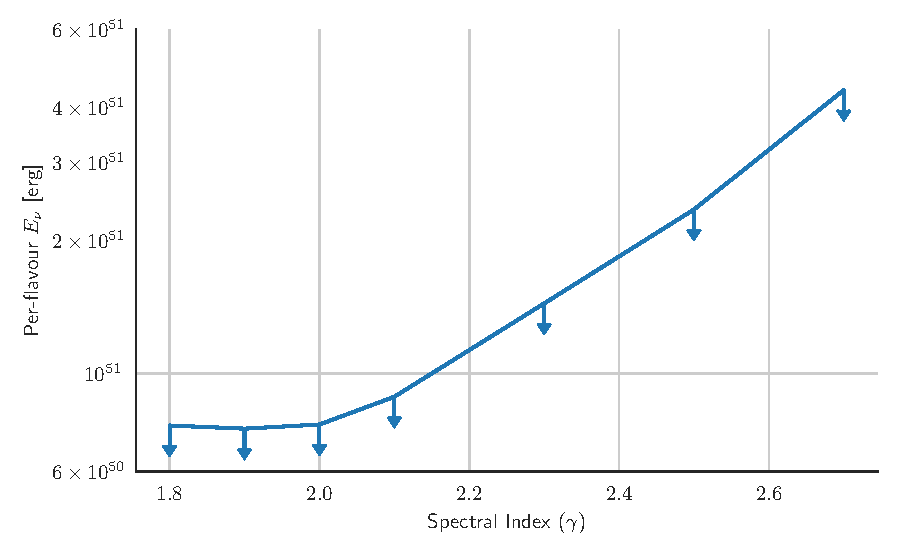
\includegraphics{results/at2018cow_limits}
	\caption{Limits on neutrino emission from AT2018cow, as a function of spectral index.}
	\label{fig:at2018cow_limits}
\end{figure}

The analysis of AT2018cow is the first example of a test for neutrino emission from FBOTs. In the time since discovery in 2018, there have been theoretical studies considering possible neutrino emission from FBOTs in general, and AT2018cow in particular \sidecite{fang_fbot}. The predicted neutrino emission is typically several orders of magnitude below the limits presented in Figure \ref{fig:at2018cow_limits}, and thus further supports the likely atmospheric origin for the neutrino excess \cite{2018ATel11785....1B}.

However, given that AT2018cow is by far the closest example of an FBOT, we can already consider the implications for the broader FBOT population emission. While initial estimates suggested that these objects might equal $\sim$4-7\% of the CCSN rate \cite{drout_fbot, fang_fbot}, these estimates have been superseded by results from magnitude-limited surveys such as ZTF, where a lack of additional FBOTs strongly suggest that the local rate must be $\sim$ 0.1\% of the CCSN rate [ADD CITATION WHEN ZTF FBOT PAPER IS OUT] 

Following the same procedure for TDEs, we find that FBOTs contribute less than 16\% of the total diffuse neutrino flux \emph{assuming that AT2018cow is representative of the broader FBOT population}. This further assumes a CCSN-like source evolution \sidecite{sfr_madau_14}, proportional to the star formation rate, and a local FBOT rate of 4 $\times$ 10$^{-7}$ Mpc$^{-3}$ yr$^{-1}$ \cite{ho_koala}. These limits are agnostic to the exact nature of FBOTs, whether they are a distinct population or a rare subgroup of some broader object class. In any case, it is clear  that any contribution of FBOTs to the diffuse neutrino flux must be subdominant.

\begin{figure}[!ht]
	\centering \includegraphics{results/fbot_limits}
	\caption{Limits on neutrino emission from FBOTs, using the limits from AT2018cow under the assumption of neutrino standard candles.}
	\label{fig:fbot_limits}
\end{figure}

\section{Robustness of Limits}

One key additional point is how robust the derived constraints are, given the many stated caveats. Full systematic studies are not typically re-performed for each individual IceCube neutrino source analysis \sidecite{ic_ps_10_yr}. This is due primarily to evidence from previous studies which demonstrated that the impact of systematic uncertainties on a typical Icecube neutrino point source search is O(\sim10\%), dominated by uncertainty on ice optical properties and DOM performance  \sidecite{ic_ps_7_yr}. This value is completely negligible in comparison to uncertainties on astrophysical population rates, as well as to additional uncertainties on the relative distribution of neutrinos across an astrophysical population. 

The searches introduced above are time-dependent analyses performed on specific windows, and are thus completely insensitive to any neutrino emission which may fall outside these windows. However, while the duration of neutrino emission may be uncertain for transients, it is expected that at least some substantial fraction of neutrino emission should occur during the periods of peak electromagnetic brightness. Thus the limits derived above can be extrapolated to cover neutrino emission models extending beyond the tested period. For example, if one predicts that only 50\% of neutrino emission from Jetted TDEs would occur in the first ~100 days, the population limit would twice as high (2.6\% rather than 1.3\%) but still constraining.

A similar argument can be applied for deviations from an unbroken neutrino power law. For TDEs this would not be surprising , because the p$\gamma$ neutrino production models introduced in Chapter \ref{ch:sources} would instead favour a peaked neutrino spectrum. However, while the energy weightings illustrated in Figure \ref{fig:mc_dec_e} are based on different power laws, the likelihood analysis will detect excesses from any neutrino spectrum. If the signal follows the same energy distribution of the background, the energy term in the Point Source Likelihood (Equation \ref{eq:ps_llh}) will provide no discriminating power, but the analysis can still identify the corresponding spatial clustering. If however there is an additional excess of neutrinos at either high or low energies, that can be well-approximated by a hard or soft neutrino power law respectively. Given that discoveries can be made with just 10-20 neutrinos, the vast majority of which will be at low energies, the ultimate difference in sensitivity for different spectra is minimal. This can be seen from Figure N, where the sensitivity is illustrated as a function of true neutrino energy. In the range X to Y, this does not vary by much, and thus any neutrino emission in this range will be strongly constrained regardless of spectrum. 

\begin{figure}[!ht]
	\centering \includegraphics{results/fbot_limits}
	\caption{Sensitivity of the Point Source Likelihood for a point source as a function of energy.}
	\label{fig:sens_disc_energy}
\end{figure}

As was demonstrated for both TDEs and FBOTs, uncertainty on the properties of a given astrophysical population remains an important source of uncertainty in constraining the overall population neutrino emission. The local rate itself remains challenging to constrain particularly for rare transient classes such as jetted TDEs or FBOTs, though wide-field time-domain surveys such as ZTF and LSST should lead to continuing improvements in precision. Constraining the rate evolution is more challenging, particularly because even deep surveys such as LSST will not probe transient rates at very high redshift where much of the neutrino emission is expected. Ultimately this source of uncertainty will likely continue to dominate limits even with next-generation neutrino detectors and transient surveys.
\setchapterimage[6.5cm]{Grid_FullView_Logo}
\setchapterpreamble[u]{\margintoc}
\chapter{Realtime Multi-Messenger Astronomy}
\labch{realtime}
\begin{fquote}[Alan Turing][Computing Machinery and Intelligence][1950]A very large part of space-time must be investigated, if reliable results are to be obtained. Otherwise we may (as most English children do) decide that everybody speaks English, and that it is silly to learn French.
\end{fquote}

In recent years, there has been a significant renewed interest in the study of transient and variable objects in astronomy. Driven primarily by the speed at which objects can evolve and disappear, particularly GRBs and latterly Kilonovae, it is often essential that astronomy can be done with minimal latency. In this vein, it is now commonplace for detectors to automatically issue so-called alerts for observations that meet given criteria, to enable other instruments to rapidly obtain near-simultaneous observations. Realtime alerts are automatically issued by GRB-searching instruments such as Swift-BAT and Fermi-GBM, while gravitaional-wave events are issued by the LIGO-VIRGO observatories, and high-energy neutrino alerts are issued by IceCube as well as ANTARES.

These alerts are all typically issued via  the Gamma-ray Coordination Network (GCN) system, where observatories can subscribe to automatically be notified or point.  An essential component of this process is the additional information published by astronomers, via GCN or Astronomers Telegrams (ATELs), in which follow-up observations are coordinated. There have been two high-profile examples of this, namely the comprehensive followup of GW170817/GRB170817A that led to the first unambiguous observation of a kilonovae, and the followup of high-energy neutrino IC170922A, which led to the identification of TXS 0506+056 as the first candidate source of TeV neutrinos. 

As part of this thesis, the author maintained and further developed the IceCube Realtime System from October 2018 onwards, acting as first responder to the vast majority of neutrino alerts in that period.

\section{The IceCube Realtime System}
The IceCube Realtime System has been operating since 2016, providing the first source of high-energy neutrino alerts. The first iteration of the alert system consisted of two streams, namely High-Energy Starting Events (HESE) and Extremely High Energy (EHE) events CITE. Each was an established event selection used to identify likely-astrophysical neutrinos cite. Filters to identify relevant events are deployed on computers at the South Pole, and detections are flagged  with low latency. After fast "online" reconstruction algorithms are applied to events, an automated machine-readable "notice" is distributed via the GCN system. In parallel, data from the event is transmitted via satellite to a computing centre in Madison, Wisconsin where a full likelihood scan is performed on the event (see chapter \ref{ch:icecube} for more details). 

Give V1 rates!

The alerts are vetted by humans to asses the event quality, with visually inspection being used to confirm classified topology and event reconstructions. The operating state of the detector is additionally checked. Following these steps, a plain-text GCN circular is distrubuted via the GCN system to confirm the good nature of the alert, and to provide the updated localisation arising from the full scan. 

This original system of alerts continued until May 2019, at which point a new alert system was implemented. While the original EHE selection was maintained, the HESE alert selection was improved to reduce the cascade contamination, and improve the astrophysical purity. In addition, a new alert stream based on the GFU event selection was initiated, with a significantly-elevated rate relative to EHE and HESE alerts. The publication of these three alert streams was unified into a new IceCube Astrotrack GCN stream, which was further subdivided into Gold and Bronze based on the average purity of alerts. Golden Astrotrack alerts will, as an ensemble, have an average of 50\% astrophysical neutrinos, while Bronze Astrotrack will have an average of 30\% astrophysical neutrinos.

The alert selections are ultimately designed based on Monte Carlo simulations, using the measured astrophysical neutrino flux and spectral index as a signal assumption. PDFs are then constructed similar to those in Figure \ref{fig:mc_dec_e} of Chapter \ref{ch:llh}, calculating signal/background ratios as a function of energy proxy and reconstructed direction, with thesholds then selected such that the integrated background contamination is <70\% (for silver) or <50\% (for gold). 

A summary of all neutrino alerts issued to date is provided in table X. Individual neutrino alerts of interest are summarised in subsequent sections. 

\subsection{IC160427A - The "PanSTARRS Supernova Neutrino"}

The first alert issued under this system, HESE alert IC160427A, was found to be in spatial coincidence with an optical transient detected by the Pan-STARRS Observatory while following up the alert. This transient was initially tentaively classified as a Type Ic supernova, for which various models have predicted neutrino emission (see Chapter \ref{ch:sources}).  However, the further spectroscopic and photometric evolution indicated that this was  more likely a Type Ia Supernova, for which no neutrino emission would be expected. Nonetheless, dedicated efforts to simulate an ensemble of IC160427A-like events led to the first characterisation of the impact of systematic uncertainties in modelling the polar glacial ice on directional reconstruction with IceCube for high-energy alerts. 

\subsection{IC170922A The "TXS 0506+056 Neutrino"}
Subsequent neutrino alerts did not yield any probable counterparts, until the detection of EHE alert IC170922A in spatial coincidence with flaring blazar TXS 0506+056. Chance coincidence in this case was estimated  This event was also resimulated in the same manner as IC160427A. Remarkably, despite its radically-different topology of through-going muon rather than starting track, the results were found to be broadly consistent. More details are given in chapter N.

\subsection{IC190331A - The "Multi-PEV Neutrino"}

A starting track was observed 

\subsection{IC190730A - The "ICRC Neutrino"}

IC190730A was a golden neutrino alert with a signalness of roughly 65\%. Following the automated notice, Millipede Reconstruction clearly showed it was well-localised, and spatially coincident with blazar PKS 1502+106. This particular blazar is extremely bright, being Nth brightest in the sky in terms of integrated gamma-ray energy flux, and owing to its high redshift of z=1.84, is one of the most luminous known blazars. This coincidence was reported in the corresponding GCN circular, and triggered a broad multi-wavelength follow-up campaign. The archival SED is provided in figure N, originally from X, but annotated to illustrate contemporaneous observations from other instruments.

\begin{figure}[!ht]
	\centering \includegraphics{pks_followup}
	\caption{The archival SED of PKS 1502+106 from X is shown. In orange, the names of various instruments that observed the source are overlaid, with orange arrows to indicate their corresponding energy regimes. CITEA-Z}
	\label{fig:PKSobs}
\end{figure}

Despite comprehensive wavelength coverage, 

The chance coincidence for at least one neutrino alert to be coincident with any of the  15 brightest blazars was calculated by the author, and found to be disfavoured at the level of 2.n sigma following the procedure in N. 

\subsection{IC190922B - The "SN2019pqh Neutrino"}

\subsection{IC191001A - The "Bran Stark Neutrino"}

\subsection{IC200107A - The "Flaring Extreme Blazar neutrino"}

\subsection{IC200530A - The "Tywin neutrino"}

\section{Interpreting high-energy neutrino alerts}

lalala

\subsection{Cluster searches}
lalaland Maybe not?

\subsection{OFU and GFU}.

Maybe not?
%
%%ztf
%

\pagelayout{wide} % No margins
\addpart{Optical follow-up with ZTF}
\pagelayout{margin} % Restore margins

\setchapterimage[8.5cm]{palomar}
\setchapterpreamble[u]{\margintoc}
\chapter{The Zwicky Transient Facility (ZTF)}
\labch{ztf}
\begin{fquote}[Fritz Zwicky][Catalogue of selected compact galaxies and of post-eruptive galaxies][1971]I soon became convinced, however, that all theorizing would be empty brain exercise and therefore a waste of time unless one first ascertained what the population of the universe really consists of, how its various members interact and how they are distributed throughout cosmic space.
\end{fquote}

The second experiment heavily utilised for the work of this thesis was the \emph{Zwicky Transient Facility} (ZTF), a `48-inch' telescope located on Mount Palomar, California. ZTF had first light in October 2017, with full survey operations beginning in March 2018. In the following chapter, the telescope itself and the ZTF data analysis chain are introduced.

\section{The ZTF Telescope}

The central design philosophy of ZTF was to \emph{maximise volumetric survey speed at fixed cost}, where volumetric survey speed describes the volume of universe observed to some absolute magnitude per unit time \sidecite{ztf_system}. Optimising volumetric survey speed requires a careful balancing of system overheads (how much time is spent preparing for an exposure), field of view (how much sky area is imaged in each exposure), and the limiting magnitude (heavily influenced by how long each exposure lasts). Maximising this quantity will then ultimately maximise the rate of optical transient detections, a key science goal of ZTF \sidecite{ztf_19_science}. This principle has guided the development of telescope hardware introduced in the following subsections.

\subsection*{Telescope Structure}

ZTF is the latest in a long line of instruments using the \emph{Samuel Oschin Telescope} \cite{ztf_system}, a Schmidt telescope located at the Palomar Observatory in California  \sidecite{harrington_52}. The Schmidt design is a common class of telescope using a curved lens known as a \emph{Schmidt corrector plate} alongside a reflecting mirror, with a curved focal plane lying within the telescope tube \sidecite{schmidt_32}. This basic design is illustrated in Figure \ref{fig:ztf_schematic}, with the golden arrows indicating the path of light. The Samuel Oschin Telescope has a 48-inch (1.2m) diameter aperture, with light focussed by the lens system and then reflected by the 1.8m primary mirror onto the ZTF camera \sidecite{ztf_obs_system}. In addition to the Schmidt Corrector plate, an additional \emph{trim plate} lens was added for the ZTF telescope, alongside additional optical elements in the camera itself. To reduce stray reflected light reaching the camera, the telescope also has a number of \emph{baffles} \cite{ztf_obs_system}. These are aluminium rings coated in non-reflecting black paint, distributed along the telescope length. 

\begin{figure}[!ht]
	\centering \includegraphics{ZTF/telescope_schematic}
	\caption{Overview of the basic Schmidt telescope design, adapted from \cite{quest_07}. The golden arrows indicate light paths.}
	\label{fig:ztf_schematic}
\end{figure}

The telescope can be rotated rapidly to point to different \emph{fields} (pre-defined on a static grid), with the time to slew between adjacent fields (separated by $\sim$7 degrees) being less than the time required to read out the camera data between exposures \cite{ztf_system}. The slewing process thus provides negligible additional overhead time. It is also entirely automated, with a dedicated robotic observing system executing the schedule for a given night. 

The telescope system also includes a robotic shutter which can open or close in <0.5s \cite{ztf_system}, with typical exposures then lasting 30s but extending up to 300s for certain observing modes. Before illuminating the ZTF camera, reflected light first passes through an optical filter. ZTF has three filters (ZTF-g, ZTF-r and ZTF-i) which are stored outside the telescope tube when not mounted, as well as a robotic arm that can exchange the mounted filter with an overhead time of $\sim$100s \cite{ztf_system}. Observations are typically conducted on the same field with multiple filters on a given night, providing colour information for detected objects.

The Schmidt design has the drawback that the camera itself blocks part of the telescope tube ($\sim$20\% for ZTF \cite{ztf_obs_system}), leading to a reduction in light throughput. To minimise this obscuration, the ZTF camera is suspended inside the telescope tube by a three-vane instrument spider, rather than e.g the four-vane spider design shown in Figure \ref{fig:ztf_schematic}.  Schmidt telescopes also have curved focal planes, so ZTF includes additional corrective optics. The camera system itself is also effectively `curved', with each of the 16 constituent pixel blocks having a unique tilt towards the focal plane \cite{ztf_system}. Ultimately, the telescope field of view spans 7.3\arcdeg (N-S) x 7.5\arcdeg (E-S) \cite{ztf_obs_system}, yielding a 55 sq. deg. area for each field. The complete process for a 30s exposure, including slewing, observation and data readout, can be completed in just 38.3s  \cite{ztf_system}. The entire ZTF system can be seen in Figure \ref{fig:ztf_diagram}.

\begin{figure}[!ht]
	\centering \includegraphics{ZTF/ztf_full}
	\caption{Overview of the ZTF telescope, adapted from \cite{ztf_obs_system}.}
	\label{fig:ztf_diagram}
\end{figure}

\subsection*{Camera}

The ZTF camera is constructed from \emph{charge-coupled devices} (CCDs). CCDs are semiconductors which store charge in potential wells that can be moved spatially, a property that is well-suited to high-resolution imaging \sidecite{boyle_70}. Incident photons transfer energy to electrons within the semiconductor, liberating charge in a process similar to the \emph{photoelectric effect} \sidecite{carroll_06, einstein_photoelectric_1905}. CCD pixels can be constructed which collect charge during an exposure, and these pixels can then be read out. Measuring the charge accumulated in a pixel over an exposure then provides a measurement of the integrated light incident on that pixel. The conversion efficiency from photons to detected electrons in a pixel is known as the \emph{quantum efficiency} (QE), and for CCDs is often $\gtrsim$80\%. 

The ZTF camera, shown in Figure \ref{fig:ztf_camera}, is composed of 16 separate CCD `wafers', each of which contains $\sim$6k x 6k pixels. The central 8 wafers employ a double-layer coating to boost QE, while the remainder have a single-layer anti-reflective coating, explaining the visible colour difference in Figure \ref{fig:ztf_camera}.

\begin{marginfigure}
	\centering \includegraphics{ZTF/ztf_fp_med}
	\caption{An image of the ZTF camera, from \cite{ztf_system}.}
	\label{fig:ztf_camera}
\end{marginfigure}

These science CCDs are mounted on a cold plate within a temperature-controlled vacuum \emph{cryostat} \cite{ztf_obs_system}. Light enters through a curved vacuum window which additionally serves as a lens. Each individual CCD then has an additional field flattener lens and is mounted with a unique tilt towards the focal plane. Within the cryostat the cold plate temperature is maintained at 165K, with $\sim$1K variations across the plate, while the CCD temperature is maintained at 170K. 

The corresponding CCD efficiency at these temperatures can be seen in Figure \ref{fig:ztf_qe}, colour-coded for the single-layer-coated CCDs (grey) and the double-layer-coated CCDs (green). The filter transmission for the ZTF-g, ZTF-r and ZTF-i filters are shown in blue, orange and red respectively. For g and r, QE remains above 80\% in the relevant 400-700nm rage for all CCDs, rising to $\gtrsim$90\% for the double-coated central CCDs. For i, there is a somewhat lower range of $\sim$80\% to $\sim$40\% across the band.

\begin{marginfigure}
	\centering \includegraphics{ZTF/QE_curves_delivered}
	\caption{The quantum efficiency of ZTF CCDs, from \cite{ztf_system}.}
	\label{fig:ztf_qe}
\end{marginfigure}

There are also four additional CCDs with $\sim$2k x 2k pixels, embedded outside the central camera, which can be seen in Figure \ref{fig:ztf_camera}. One of these outer CCDs acts as a guiding camera, to ensure pointing accuracy by identifying the position of reference stars. The remaining CCDs each have a differently offset from the camera, and are collectively used to infer the extent of optical aberrations from atmospheric turbulence \sidecite{tokovinin_06}. The entire cryostat structure is shown in Figure \ref{fig:cryostat_exploded}.

\begin{figure*}
	\centering \includegraphics{ZTF/cryostat_exploded}
	\caption{The ZTF cryostat design, from \cite{ztf_system}.}
	\label{fig:cryostat_exploded}
\end{figure*}

Each CCD is split into four distinct quadrants, with each of these 64 quadrants then having an independent set of readout electronics. Gaps between the camera CCDs give an instrumented focal plane fill factor of 86.7\%, thus yielding a 47.6 sq. deg field of view for each ZTF exposure. This can be seen in Figure \ref{fig:ztf_footprint}, with the predecessor PTF/iPTF camera and other surveys provided for comparison. The moon and nearby galaxy Andromeda are also shown for scale.

\begin{figure*}
	\centering \includegraphics{ZTF/fov}
	\caption{The ZTF camera footprint, from \cite{laher_18}.}
	\label{fig:ztf_footprint}
\end{figure*}

\section{ZTF Scheduling and Surveys}
\label{sec:survey}

ZTF observations are handled within the framework of a \emph{primary grid}, with which the sky is divided into a grid of pre-defined \emph{fields}. This primary grid covers 87.5\% of the accessible sky once camera chip gaps are accounted for \sidecite{ztf_survey_19}. There is also a \emph{secondary grid}, offset diagonally from the primary grid to minimise chip gap overlap, yielding a combined 99.2\% coverage of the accessible sky. ZTF sequentially observes these fields, in an order determined by a scheduler. 

ZTF executes a number of different surveys concurrently, each of which contributes a set of \emph{requests} for observations of particular fields, with all programs interwoven into a single mixed field observation queue for a given night. The ZTF scheduler optimises the ordering and field prioritisation with the aim of maximising the spatial volume probed by exposures in a given night, subject to the constraint that these must be balanced over a given calendar month \cite{ztf_survey_19}. With this framework nearby fields are observed successively as this minimises slew time, while low-airmass observations are prioritised since these probe larger volumes. This metric also encompasses the overhead lost due to filter exchanges ($\sim$2 mins), optimising the timing and minimising the frequency of these exchanges over a night. The scheduling algorithm is fast enough to allow the schedule to be repeatedly recalculated in response to external factors such as periods of poor weather.

The original observing time allocation was made for the initial survey (ZTF-I) from October 2017 - September 2020 on the basis of various funding contributions, while the successor survey ZTF-II (from October 2020 onwards) involved an updated survey allocation based on new funding commitments.

Roughly 40\% of the ZTF-I observing time was allocated to a public survey funded by an award from the NSF Mid-Scale Innovations Program, the so-called ``MSIP public survey'' \cite{ztf_survey_19}. Most MSIP time was allocated to an extragalactic \emph{Northern Sky Survey}, covering all primary fields with centres at galactic latitude |b| > 7$\arcdeg$ and declination $\delta \geq$ -31$\arcdeg$. All accessible fields in the Northern Sky Survey were observed with a 3-day cadence in both g and r on the same night, with a separation of at least 30 mins for rejection of moving objects. ZTF-II features an enlarged Northern Sky Survey covering 50\% of the observing time, with an increased 2-day observation cadence \sidecite{ztfii_graham_20}. These surveys provide a comprehensive accounting of the dynamic transient sky, and were a vital component of the neutrino follow-up program introduced in Chapter \ref{ch:ztf_too}.

Another 40\% of the ZTF-I observing time was allocated to \emph{partnership time}, as well as 30\% of ZTF-II time \cite{ztf_survey_19, ztfii_graham_20}. The exact observation strategy for partnership time changed over the course of ZTF project, with regular calls for new proposed observation programs. Of particular importance for this thesis was the allocation for \emph{Target-of-Opportunity} (ToO) observations, conducted in response to external triggers such as neutrinos, gravitational waves and gamma-ray bursts (see Chapter \ref{ch:ztf_too}). Time was awarded to such observations in all partnership allocations to date. Because of their time-sensitive nature, these ToO observations interrupt the automated ZTF schedule.

Finally 20\% of ZTF-I and ZTF-II observations are dedicated to \emph{Caltech time}, with an emphasis on strategies not covered by other surveys such as high-cadence observations searching for fast transients \cite{ztf_survey_19, ztfii_graham_20}. Data from these observations are accessible only to Caltech scientists, and thus were not incorporated into this thesis.

\section{ZTF Data Processing}

The raw image data is read out from the camera CCDs on Mount Palomar, and transferred to \emph{Infrared Processing and Analysis Center} (IPAC) in Pasadena, California \sidecite{ztf_data_processing}. This transfer typically takes <25s \cite{ztf_system}. The images are then decompressed, and split into individual quadrants. 

Because the telescope performance can vary substantially between nights and exposures, for example due to variations in temperature or electronic noise, each new image must be calibrated. The various data processing steps are outlined in the following subsections. Some calibration stages require specific observations newly taken each night, while others are unique steps performed separately for each exposure and quadrant. The full calibration procedure is illustrated in Figure \ref{fig:ztf_calibration}.

\begin{figure}[!ht]
	\centering \includegraphics{ZTF/ztf_calibration}
	\caption{The full ZTF calibration process, from \cite{ztf_data_processing}.}
	\label{fig:ztf_calibration}
\end{figure}

\subsection*{Overscan Correction}

CCD cameras typically contain an \emph{overscan region}, consisting of CCD pixels at the edge of a wafer which are not illuminated by light during an exposure. These pixels provide specific calibration data for each individual exposure and quadrant, by measuring the base telescope response during a particular exposure in the absence of light. By measuring the signal in each overscan pixel, an interpolated baseline can be calculated by fitting a 2D polynomial to the overscan data \cite{ztf_data_processing}. This baseline is then subtracted from all images as a first processing step, a method known as \emph{overscan correction}. 

\subsection*{Bias Correction}

The next calibration stage involves taking overscan-corrected \emph{bias images}. These are `zero exposure' images which measure the base telescope electronics response in the absence of any integrated exposure time, providing the charge floor in each pixel. For ZTF, at least 20 such bias images are taken each night prior to observing, with these images then stacked to provide an average per-pixel bias \cite{ztf_data_processing}. A dedicated bias image is created for each CCD quadrant, and is then subtracted from all science images made that night using the CCD quadrant.

\subsection*{Flat Field Correction}

The next step is the \emph{flat field correction}, in which a known light signature is passed through the telescope, with camera performance then measured to identify any variations in response. For ZTF, there is a dedicated \emph{Flat Field Illuminator} consisting of a reflective screen inside the dome \cite{ztf_system}. This screen is illuminated by 24 LEDs, covering a range of wavelengths, enabling the detector response to be mapped across the required ZTF filters. 

%\begin{figure}[!ht]
%	\centering \includegraphics{ZTF/ZTF_FFI_in_dome}
%	\caption{The ZTF Flat Field Illuminator, from \cite{ztf_obs_system}.}
%	\label{fig:ztf_ffi}
%\end{figure}

New bias-corrected flat field images are taken nightly before survey operations begin, with a separate image for each quadrant and filter.  Much like for bias images, at least 20 separate images are taken and then stacked together to create the final flat field images. Each quadrant science image is then divided by the respective flat field image to normalise the response in each pixel. Systematic variations of $\sim$2.5\% have been observed between nights, and without calibration these variations would otherwise impact photometric precision \cite{ztf_data_processing}. 

\subsection*{Astrometric Calibration}

The science images must then be calibrated for \emph{astrometry}, in which the exact sky position of each telescope pixel is derived. For ZTF, this is conducted using data from the most recent \emph{Gaia} catalogue \sidecite{gaia_dr1, gaia_dr2}. \emph{Gaia} is a space-based optical survey that provides a comprehensive stellar census of the local universe, with data releases containing high-precision data on the position ($\sim$0.1 mas) and luminosity of stars with an apparent magnitude brighter than G=21 \cite{gaia_dr2}. There are $\sim$1.7 billion catalogued objects in DR2, with \emph{proper motion} also calculated for the majority of stars. Though the limiting magnitude is comparable to that of ZTF, Gaia is used for astrometric calibration because it has superior pointing accuracy due to a lack of atmospheric scattering/absorption for the satellite.

Each new ZTF science image is analysed using `source extractor' software (unfortunately named \emph{SExtractor} \sidecite{sextractor_96}), to identify sources and fit a \emph{Point Spread Function} (PSF) to each of these objects \cite{ztf_data_processing}. Bright (12 $\leq$ G $\leq$ 18) catalogued stars that have been pre-selected for each ZTF field quadrant are then matched to these sources, using the \emph{Scamp} software package \sidecite{scamp_06}. By comparing the ZTF-derived position of these stars to their `true' Gaia-derived ones, a full \emph{astrometric solution} can be found for each ZTF image, enabling a precise calibration of the sky position corresponding to each pixel in the image.

\subsection*{Photometric Calibration}

Following the calibration of positioning, images then undergo \emph{photometric calibration}. This process involves comparing the observed signal from catalogued stars to their known flux, from which the brightness of other objects can then be inferred. For photometric calibration, ZTF uses data from the first data release of the \emph{Pan-STARRs} survey (PS1) \sidecite{panstarrs_16}. Photometrically stable stars are selected (with consistent photometry across the multi-epoch PS1), with additional cuts to mitigate source confusion by excluding stars with nearby neighbours \cite{ztf_data_processing}. PS1 serves as a suitable calibration catalogue because it uses filters similar to ZTF with a substantially deeper limiting magnitude (>23 mag for g/r/i).

Much like for astrometry, the photometric calibrator star list is pre-selected for each ZTF field quadrant, with each science image then being calibrated separately based on this list \cite{ztf_data_processing}.  The calibrator list is cross matched to the sources extracted by \emph{SExtractor} in each quadrant during the astrometric calibration stage. It is assumed that the photometric bias can be parameterised as:

\begin{equation}
	m_{\textup{diff, f}} \equiv m_{\textup{PS1, f}} - m_{\textup{ZTF, f}} = ZP_{\textup{f}} + \left( c_{\textup{f}} \times PS1_{\textup{clr, f}} \right)
	\label{eq:photmetric_calibration}
\end{equation}

where f is the filter, ZP$_{\textup{f}}$ is the \emph{calibration zero point} for that filter, $c_{\textup{f}}$ is an empirical constant and $PS1_{\textup{clr, f}}$ is an estimate of the star colour from PS1 data. The $PS1_{\textup{clr, f}}$ term gives the local colour gradient, defined as the difference in apparent magnitude between the relevant PS1 filter and one adjacent filter:

\begin{itemize}
	\item ($m_{\textup{g}} - m_{\textup{r}}$) for g-band and r-band images
	\item ($m_{\textup{r}} - m_{\textup{i}}$) for i-band images
\end{itemize}

By calculating the $m_{\textup{diff, f}}$ value for all photometric calibrator stars in a quadrant, and then globally fitting these deviations to minimise $m_{\textup{diff, f}}$ using Equation \ref{eq:photmetric_calibration}, a value for the calibration zero point ZP$_{\textup{f}}$ and colour constant $c_{\textup{f}}$ can be derived for each quadrant of a science image. Having determined these values, Equation \ref{eq:photmetric_calibration} can then be used to calibrate the photometry of all other sources not included in the photometric calibrator list.

\subsection*{Image Artefacts}

ZTF images must also be corrected to remove various image artefacts, with different artefact classes targeted at specific processing stages (see Figure \ref{fig:ztf_calibration}). The following artefact classes are flagged:

\begin{itemize}
	\item\emph{Saturated pixels} are individual bright pixels that become charge-saturated, at which point they are no longer useful for image subtraction. This process provides an effective upper limit on source fluxes to which ZTF is sensitive, though variations in image quality between exposures can lead to different saturation flux thresholds \cite{ztf_data_processing}.
	\item \emph{Bad pixels} are those for which signals are untrustworthy. Some bad pixels are known in advance and masked, but further suspicious pixels with high variability are flagged through bias image analysis \cite{ztf_data_processing}. 
	\item \emph{Image streaks} can also be observed due to the movement of Near Earth Objects (NEOs) or Solar System Objects (SSOs) over the sky during an exposure. These streaks are flagged by dedicated machine learning algorithms  \sidecite{ztf_ml_19}.
	\item \emph{Ghosts} can arise from secondary reflections of bright sources in an image \sidecite{yang_02}.
	\item \emph{Cosmic rays} passing through the CCD can ionise nearby pixels, leading to a handful of bright pixels in an image.
\end{itemize}

After this stage the images are fully calibrated, and are then referred to as \emph{science images}. 

\subsection*{ZTF On-Sky Performance}

Following calibration, the 5$\sigma$ limiting magnitude can be estimated for each quadrant in a science image using a model for the detector response function and then computing the median magnitude of sources lying at the 4.5 $\leq$ S/N $\leq$ 5.5 detection threshold \cite{ztf_data_processing}. For ZTF with 30s exposures, the median limiting magnitude is 20.8 for g-band, 20.6 for r-band and 19.9 for i-band, with some dependence on the lunar cycle phase \cite{ztf_system}. The \emph{image quality} can also be derived by looking at distant sources which are intrinsically point-like, and observing the apparent spatial distribution of the corresponding flux in ZTF images, yielding a  PSF for that object. For observations above airmass 1.2, sources have a typical PSF \emph{Full Width Half Maximum} (FWHM) of 2.1\arcsec in g-band , 2.0\arcsec in r-band and 2.1\arcsec in i-band \cite{ztf_system}.

\subsection*{Reference Images}

Whereas science images provide an instantaneous view of the night sky on a given night, \emph{reference images} are created to give a comprehensive map of the static night sky baseline. By comparing science images to reference images, changes in flux from transient or variable sources can be identified. For ZTF, IPAC built reference images for each field and filter using early survey data. These reference images are composed of deep composite images containing at least 15 \emph{coadded} (stacked) individual science images taken under optimal observing conditions \cite{ztf_data_processing}. Each constituent science image was calibrated using the same processing substeps as outlined above.

\subsection*{Image Subtraction}

Much like for science images, \emph{SExtractor} source extraction is also performed on reference images to derive source PSFs. Both sets of PSFs (science and reference) are then used by the \emph{SWarp} software package \sidecite{swarp_02} to create an interpolation of the reference image projected onto the science image. The \emph{ZOGY algorithm} is then used to perform \emph{image subtraction}, where the interpolated reference image is subtracted from the science image \sidecite{zogy_16}. The resulting data product is known as a \emph{difference image}, and contains deviations between the science image and reference image arising from transient or variable sources. The threshold for a `significant detection' is set at S/N=5, with the algorithm identifying both flux increases (positive subtractions) and flux decreases (negative subtractions). 

An example of the subtraction process is shown in Figure \ref{fig:ztf_scirefdif}, based on alert data from 2018 June 19 for ZTF transient \emph{AT2018cow} (see Chapter \ref{ch:results}). The extended host galaxy is visible in both science and reference images, alongside one bright nearby object below and two additional faint objects to the right. There is a very bright excess in the science image, outshining the host galaxy, which was not present in the reference image. This can be seen even more clearly in the difference image, where a single bright gaussian-like PSF is seen. This PSF belongs to the transient, and is used to calculate the transient flux in that epoch and filter.

\begin{figure}
	\centering \includegraphics{ZTF/scirefdif}
	\caption{ZTF science, reference, and difference images for AT2018cow.}
	\label{fig:ztf_scirefdif}
\end{figure} 

\subsection*{Candidate Creation}

Having identified such high-significance excesses in difference images, loose quality cuts are then applied to each \cite{ztf_data_processing}. One key stage involves applying machine learning to the difference image data to assign a score for subtraction quality (the so-called \emph{RealBogus score}), enabling spurious detections arising from poor subtractions to be flagged \cite{ztf_ml_19}. Those detections passing all cuts are then formally dubbed \emph{candidates}. These new candidates are cross-matched to a database of recent candidates, linking new detections with any previous detections of the same object, and assigned a unique ZTF name if none exists. Upper limits are also calculated for recent images without significant detections of a candidate. 

Additional contextual information is found by cross-matching candidates to external catalogues such as data releases of the \emph{Gaia} or \emph{Pan-STARRs} surveys. Machine learning is also applied to determine whether nearby catalogued objects are more likely to be stars or galaxies (the \emph{StarGalaxy score}) \sidecite{ztf_stargalaxy_18}. Images are tagged by the program under which they were observed (see Section \ref{sec:survey}), to ensure consistent data access rights downstream. All of this data is then passed to the ZTF Alert Distribution System. The median duration from exposure to completed data processing is 8.5 minutes, with 90\% of detections processed within 12.6 minutes \cite{ztf_data_processing}.

\subsection*{ZTF Alert Distribution System}

The distribution of ZTF survey data is handled by the \emph{ZTF Alert Distribution System} (ZADS) \sidecite{zads_19}. ZTF ultimately detects $\sim$1 million candidates each night, with an average of $\sim$11.5 detections per image CCD quadrant \cite{ztf_data_processing}. To manage this large data volume each candidate detection is packaged as an \emph{alert} using the \emph{Apache Avro} format\footnote{\url{https://avro.apache.org}}. These alerts contain all the relevant metadata introduced above such as detection history and properties of the difference image PSF. They also contain the additional contextual data, as well as cutouts of the three calibrated images (science, reference and subtraction) such as those shown in Figure \ref{fig:ztf_scirefdif}.

 These alerts are then distributed as part of an \emph{alert stream}, to which external machines can `listen' to receive the data. Due to the size of the three images, each alert is typically $\sim$60 kB, yielding a nightly data volume of $\sim$70 GB in the alert stream.  

The original data stream transfers data from IPAC to the University of Washington (UW), where the data is then backed up \cite{zads_19}. The entire data stream is also published nightly at UW. Additional \emph{Event Brokers} can also listen to the alert stream, with these brokers being responsible for providing data access to the wider userbase. To handle differentiated data access (see Section \ref{sec:survey}) there is both a `public' stream (containing only public alerts)  and a  `partnership' stream (containing both partnership and public alerts). For this thesis, the latter stream provided the relevant data.

\section{Ampel}

For this thesis, access to ZTF data occurred primarily through \emph{Ampel}. Ampel is an open-source  software framework, developed by the ZTF groups at DESY Zeuthen and HU Berlin \sidecite{ampel}. The name refers to the initial scope of the software, handling Alert Management, Photometry and Evaluation of Light Curves (AMPEL). This Ampel software framework was used to perform the alert filtering for the \ztf ~introduced in Chapter \ref{ch:ztf_too}.

The Ampel framework is modular, performing four distinct \emph{tiers} (stages) of data processing:

\begin{itemize}
	\item \textbf{Tier 0 - Filter} - Selects the relevant alerts from a larger alert stream
	\item \textbf{Tier 1 - Update} - Identifies any corrections to apply to alert data, and crossmatches to data from any other alert streams
	\item \textbf{Tier 2 - Calculate} - Performs analysis on alert data, to calculate specific outputs
	\item \textbf{Tier 3 - Respond} - Connects the output of the analysis to the external world
\end{itemize}

For each step, the base structure is defined, with users able to contribute personalised modules based on one of these four template layers. An alert stream is provided as a starting input, which is then filtered by a Tier 0 module to select only those objects which are `interesting' for a particular science user. In principle, the alert data would then cross-matched to alert data from other instruments at the Tier 1 stage, but this is presently a theoretical step because Ampel only handles ZTF alerts. After this, any selected Tier 2 modules will be run to analyse data. Such modules could, for example, perform lightcurve analysis or cross-matching to external catalogues. Finally, this processed data is then connected to the outside world with one or more Tier 3 modules. Examples include pushing data to an external database, or pushing a high-level summary to a website. 

\begin{figure}[!ht]
	\centering \includegraphics[trim={0 1cm 0 3cm},clip]{ZTF/ampel_intro}
	\caption{A schematic of the Ampel data pipeline, from \cite{ampel}.}
	\label{fig:ampel_pipeline}
\end{figure}

In addition to the software framework itself, the name \emph{Ampel} can also refer to the dedicated computer infrastructure running at DESY Zeuthen. As illustrated in Figure \ref{fig:ampel_pipeline}, Ampel serves as a broker, subscribing to the UW alert stream and transmitting data downstream to science users. There is a live instance of the Ampel software running at DESY that processes the ZTF partnership stream, and also hosts a number of user-defined filters from the wider collaboration. 

Of particular relevance for this thesis is the dedicated \emph{Ampel archive database}, in which all ZTF alerts are compressed and archived. The archive database can be efficiently queried by object name or spatial coordinates, providing quick access to historical ZTF data at a given position. Due to the unique selection function required for each external trigger, the \ztf ~relies on data from the archive database to `replay' old alerts. The median latency from shutter close to data availability in Ampel is under 10 minutes, though upstream delays at IPAC can increase this in some cases.

\setchapterimage[8.5cm]{palomar}
\setchapterpreamble[u]{\margintoc}
\chapter{Transient Follow-up with ZTF}
\labch{ztf_too}
\begin{fquote}[Oscar Wilde][Lady Windermere's Fan][18??]We are all in the gutter, but some of us are looking at the stars
\end{fquote}

The motivation for all real-time analysis and prompt follow-up observations of external triggers is to obtain contemporaneous data. Put another way, these observations are designed to quickly identify time-dependent transient or variable activity which would be missed by untargeted survey operations.  In the case of GW and short GRB follow-up, searches are targeted towards identifying kilonovae (KNe), of which GW170817/AT2017gfo was a spectacular well-documented first example. These KNe are inherently fast-evolving transients which will by definition not be present before the extrenal trigger. For neutrinos, there are a proliferation of possible optical transients (e.g GRBs, TDEs, SNe) and variable objects (primarily blazars) which could be identified in an optical follow-up observations. In both cases, a handful of potentially interesting extragalactic objects will need to be selected against a vast background of spurious detections, and unrelated galactic or solar-system objects.

\section{The Ampel Follow-up Pipeline}
Given the similar challenge, a single flexible analysis, the \ztf, was developed by the author to identify candidate counterparts to GW, GRB and neutrino trigger events. ZTF is particularly well-suited to this type of extragalactic transient discovery,  because ZTF routinely images the visible Northern Sky once every three nights to a median depth of $20.5^{m}$ as part of a public survey \sidecite{ztf_survey_19}.  This provides an extensive base to distinguish between new transients that could be coincident with an external trigger, and those with previous detections. The large volumetric survey speed of ZTF often provides significant serendipitous coverage of events. This wide-field cadence can however be supplemented by dedicated Target-of-Opportunity (ToO) observations scheduled for a particular trigger through the GROWTH ToO Marshal \sidecite{coughlin_19}. 

As introduced in Chapter \ref{ch:ztf}, all ZTF science images are processed, significant detections are extracted, and these are archived in a database at DESY as part of the local computer infrastructure (the \emph{archive database}). External triggers, which come in the form of probability skymaps or GCN circulars, are downloaded and parsed with \ztf. The archive database is then queried for coincident alerts, using either temporal indexing or spatial indexing depending on the size of the target region. Once loaded, these alerts are then filtered by the \ztf~using \emph{AMPEL} \sidecite{ampel}, a platform for realtime analysis of multi-messenger astronomy data. Our selection is based on an algorithm for identifying extragalactic transients \cite{ampel}. In order to identify candidate counterparts, we apply the following cuts to ToO and survey data:

\begin{itemize}
	\item We reject likely subtraction artefacts using machine learning classification and morphology cuts \sidecite{ztf_ml_19}. Subtractions must be positive, i.e a candidate must be brighter than the same position in stacked reference images.
	\item We reject solar system objects through matches to known catalogues \cite{ztf_ml_19}. We further remove uncatalogued solar system objects by requiring multiple detections for each candidate at the same location, separated temporally by at least 15 minutes, thereby rejecting moving objects.
	\item We reject galactic stellar sources by removing detections cross-matched to objects with measured parallax in the second data release of the \emph{GAIA} satellite \sidecite{gaia_dr2}. Objects are rejected if they have non-zero parallax with a significance of at least 3$\sigma$. We further reject likely stars with machine learning classifications, based on sources detected by Pan-STARRS1 \sidecite{ztf_stargalaxy_18}, removing those objects with an estimated stellar probability greater than 80\%. 
	\item We reject AGN variability by cross-matching objects to the WISE survey. We identify likely AGN by applying a series of cuts based on measured IR colour \sidecite{wise_10}.
	\item We rejected unassociated objects by requiring both spatial and temporal coincidence with a given trigger.
\end{itemize}

These cuts typically yield $\sim$0.2 candidates per square degree of sky. Promising candidates are prioritised for spectroscopic classification, to confirm or rule out a possible association with a given neutrino. 

\section{Neutrino Follow-up Program}
ZTF has since its inception had a dedicated program to identify sources of high-energy astrophysical neutrinos, through targeted follow-up observations. A significant component of this thesis was the initial development and operation of this neutrino follow-up program. Given the proliferation of proposed source classes, neutrino follow-up are characterised by searching relatively well-localised regions for poorly-defined objects. This is particularly true for optical follow-up, where potential counterparts include Tidal Disruption Events (TDEs), Type IIn or choked jet SNe, kilonovae, GRB afterglows, superluminous supernovae (SLSNe) or blazar flares (see Chapter \ref{ch:sources} for a comprehensive list). While pre-neutrino detections could rule out neutrino production from choked jet supernovae, in most cases we do not even have stringent constraints in when neutrinos may be expected.

For neutrinos, spatial and temporal coincidence is ensured by requiring that an object lies within the reported 90\% localisation rectangle from IceCube, and being detected at least once following the neutrino arrival time. We have followed up N neutrinos in the period from survey start on 2018 March 20 to 2020 June 31, out of a total of N neutrino alerts published by IceCube. Table \ref{tab:nu_alerts} summarises each neutrino alert that has been observed by ZTF. From 2019 June 17, IceCube published neutrino alerts with improved selection criteria to provide an elevated alert rate \sidecite{ic_realtime_19} (see Chapter \ref{ch:realtime} for more details). In addition to 1 of the 12 alerts under the old V1 selection, ZTF followed up 7 of the 19 alerts published under the V2 selection. In general, we aim to follow all well-localised neutrinos of likely astrophysical origin reported by IceCube which are visible to ZTF and can be observed promptly. 
 
Those alerts not observed by ZTF are summarised in Table \ref{tab:nu_non_observed}. Of those 23 alerts not followed up by ZTF, the primary reasons were proximity to the Sun (8/23), alerts with poor localisation and low astrophysical probability (6/23) and alert retraction (4/23). For events which were reported with estimates of astrophysical probability, we chose not to follow up those that had both low astrophysical probability ($<$ 50\%) and large localisation regions ($>$ 10 sq.\,deg.). This value was not reported for high-energy starting events (HESE) under the old IceCube alert selection, nor for one alert, IC200107A, that was identified outside of the standard alert criteria \sidecite{ic200107a} (see also Chapter \ref{ch:realtime}). The full breakdown of neutrino observations statistics can be seen in Figure N.
 
 Each neutrino localisation region can typically be covered by one or two ZTF observation fields. Multiple observations are scheduled for each field, with both $g$ and $r$ filters, and a separation of at least 15 minutes between images. These observations typically last for 300~s, with a typical limiting magnitude of $21.0^{m}$.  ToO observations are typically conducted on the first two nights following a neutrino alert, before swapping to serendipitous coverage as part of the public survey. 
 
 \begin{figure}[!ht]
 	\centering \includegraphics{ztf_too/pie}
 	\caption{Breakdown of the neutrino follow-up program, as of 2021 June 25. }
 	\label{fig:pie}
 \end{figure}
 
 MENTION THAT COMMISSIONING ONE
 
 \begin{table*}
 	\centering
 	\begin{tabular}{||c c c c c c c ||} 
 		\hline
 		\textbf{Event} & \textbf{R.A. (J2000)} & \textbf{Dec (J2000)} & \textbf{90\% area} & \textbf{ZTF obs} &~ \textbf{Signalness}& \textbf{Ref}\\
 		& \textbf{(deg)}&\textbf{(deg)}& \textbf{(sq. deg.)}& \textbf{(sq. deg.)} &&\\
 		\hline
 		IC190503A & 120.28 & +6.35 & 1.94& 1.37 & 36\%&\cite{ic190503a, ic190503a_ztf}\\
 		IC190619A & 343.26 & +10.73 & 27.16& 21.57 & 55\%&\cite{ic190619a, ic190619a_ztf}\\
 		IC190730A & 225.79 & +10.47 & 5.41& 4.52 & 67\%&\cite{ic190730a,ic190730a_ztf}\\
 		IC190922B & 5.76 & -1.57 & 4.48 & 4.09 & 51\%&\cite{ic190922b, ic190922b_atel, ic190922b_ztf}\\
 		\textbf{IC191001A} & \textbf{314.08} & \textbf{+12.94} & \textbf{25.53} & \textbf{20.56} & \textbf{59\%}& \textbf{\cite{ic191001a,ic191001a_atel, ic191001a_ztf}}\\
 		IC200107A & 148.18 & +35.46 & 7.62 & 6.22 & - &\cite{ic200107a,ic200107a_ztf}\\
 		IC200109A & 164.49 & +11.87 & 22.52 & 20.06 & 77\%&\cite{ic200109a,ic200109a_ztf}\\
 		IC200117A & 116.24 & +29.14 & 2.86 &  2.66 & 38\%&\cite{ic200117a,ic200117a_ztf, ic200117a_ztf_2}\\
 		\hline
 	\end{tabular}
 	\caption{Summary of the eight neutrino alerts followed up by ZTF. IC191001A is highlighted in bold. The 90\% area column indicates the region of sky observed at least twice by ZTF, within the reported 90\% localisation, and accounting for chip gaps. The \textit{signalness} estimates the probability that each neutrino is of astrophysical origin, rather than arising from atmospheric backgrounds.}
 	\label{tab:nu_alerts_old}
 \end{table*}

\begin{table*}
	\centering
	\begin{tabular}{||c c c c c c c ||} 
		\hline
		\textbf{Event} & \textbf{R.A. (J2000)} & \textbf{Dec (J2000)} & \textbf{90\% area} & \textbf{ZTF obs} &~ \textbf{Signalness}& \textbf{Ref}\\
		& \textbf{[deg]}&\textbf{[deg]}& \textbf{[sq. deg.]}& \textbf{[sq. deg.]} &&\\
		\hline
		IC190503A & 120.28 & +6.35 & 1.9 & 1.4 & 36\% & \cite{ic190503a, ic190503a_ztf} \\ 
		IC190619A & 343.26 & +10.73 & 27.2 & 21.6 & 55\% & \cite{ic190619a, ic190619a_ztf} \\ 
		IC190730A & 225.79 & +10.47 & 5.4 & 4.5 & 67\% & \cite{ic190730a, ic190730a_ztf} \\ 
		IC190922B & 5.76 & -1.57 & 4.5 & 4.1 & 51\% & \cite{ic190922b, ic190922b_ztf} \\ 
		IC191001A & 314.08 & +12.94 & 25.5 & 20.6 & 59\% & \cite{ic191001a, ic191001a_ztf} \\ 
		IC200107A & 148.18 & +35.46 & 7.6 & 6.2 & - & \cite{ic200107a, ic200107a_ztf} \\ 
		IC200109A & 164.49 & +11.87 & 22.5 & 20.1 & 77\% & \cite{ic200109a, ic200109a_ztf} \\ 
		IC200117A & 116.24 & +29.14 & 2.9 & 2.7 & 38\% & \cite{ic200117a, ic200117a_ztf, ic200117a_ztf2} \\ 
		IC200512A & 295.18 & +15.79 & 9.8 & 9.3 & 32\% & \cite{ic200512a, ic200512a_ztf} \\ 
		IC200530A & 255.37 & +26.61 & 25.3 & 22.0 & 59\% & \cite{ic200530a, ic200530a_ztf, ic200530a_ztf2} \\ 
		IC200620A & 162.11 & +11.95 & 1.7 & 1.2 & 32\% & \cite{ic200620a, ic200620a_ztf} \\ 
		IC200916A & 109.78 & +14.36 & 4.2 & 3.6 & 32\% & \cite{ic200916a, ic200916a_ztf, ic200916a_ztf2} \\ 
		IC200926A & 96.46 & -4.33 & 1.7 & 1.3 & 44\% & \cite{ic200926a, ic200926a_ztf} \\ 
		IC200929A & 29.53 & +3.47 & 1.1 & 0.9 & 47\% & \cite{ic200929a, ic200929a_ztf} \\ 
		IC201007A & 265.17 & +5.34 & 0.6 & 0.5 & 88\% & \cite{ic201007a, ic201007a_ztf} \\ 
		IC201021A & 260.82 & +14.55 & 6.9 & 6.3 & 30\% & \cite{ic201021a, ic201021a_ztf} \\ 
		IC201130A & 30.54 & -12.10 & 5.4 & 4.5 & 15\% & \cite{ic201130a, ic201130a_ztf} \\ 
		IC201209A & 6.86 & -9.25 & 4.7 & 3.2 & 19\% & \cite{ic201209a, ic201209a_ztf} \\ 
		IC201222A & 206.37 & +13.44 & 1.5 & 1.0 & 53\% & \cite{ic201222a, ic201222a_ztf} \\ 
		IC210210A & 206.06 & +4.78 & 2.8 & 2.1 & 65\% & \cite{ic210210a, ic210210a_ztf} \\ 
		IC210510A & 268.42 & +3.81 & 4.0 & 4.0 & 28\% & \cite{ic210510a, ic210510a_ztf} \\ 
		
		\hline
	\end{tabular}
	\caption{Summary of the 21 neutrino alerts followed up by ZTF since survey start on 2018 March 20.}
	\label{tab:nu_alerts}
\end{table*})

 
 \begin{table*}
 	\centering
 	\begin{tabular}{||c c ||} 
 		\hline
 		\textbf{Cause} & \textbf{Events} \\
 		\hline
 		\textbf{Alert Retraction} & IC180423A\cite{ic180423a}, IC181031A\cite{ic181031a}, IC190205A\cite{ic190205a}, IC190529A\cite{ic190529a}\\
 		\hline
 		\textbf{Proximity to Sun} &IC180908A\cite{ic180908a}, IC181014A\cite{ic181014a}, IC190124A\cite{ic190124a}, IC190704A\cite{ic190704a}\\
 		& IC190712A\cite{ic190712a}, IC190819A\cite{ic190819a}, IC191119A\cite{ic191119a}, IC200227A\cite{ic200227a}\\
 		\textbf{Low Altitude} & IC191215A\cite{ic191215a}\\
 		\textbf{Southern Sky} & IC190331A\cite{ic190331a}, IC190504A\cite{ic190504a}\\
 		\hline
 		\textbf{Poor Signalness \& Localisation} &
 		IC190221A\cite{ic190221a}, IC190629A\cite{ic190629a}, IC190922A\cite{ic190922a}\\
 		& IC191122A\cite{ic191122a}, IC191204A\cite{ic191204a}, IC191231A\cite{ic191231a}\\
 		\hline
 		\textbf{Bad Weather} & IC200120A\cite{ic200120a,ic200120a_2}\\
 		\textbf{Telescope Maintenance} & IC181023A\cite{ic181023a}\\
 		\hline
 	\end{tabular}
 	\caption{\textbf{Summary of the 23 neutrino alerts that were not followed up by ZTF since survey start on 2018 March 20.} Of these, 4/23 were retracted, 11/23 were inaccessible to ZTF for various reasons, 6/23 were deemed alerts of poor quality, while just 2/23 were alerts that were missed although they passed our criteria.}
 	\label{tab:nu_non_observed_old}
 \end{table*}

\begin{table*}
	\centering
	\begin{tabular}{||c c ||} 
		\hline
		\textbf{Cause} & \textbf{Events} \\
		\hline
		Alert Retraction & IC180423A \cite{ic180423a}, IC181031A \cite{ic181031a}, IC190205A \cite{ic190205a}, IC190529A \cite{ic190529a} \\ 
		& IC200120A \cite{ic200120a}, IC200728A \cite{ic200728a}, IC201115B \cite{ic201115b}, IC210213A \cite{ic210213a} \\ 
		& IC210322A \cite{ic210322a}, IC210519A \cite{ic210519a} \\ 
		\hline 
		Proximity to Sun & IC180908A \cite{ic180908a}, IC181014A \cite{ic181014a}, IC190124A \cite{ic190124a}, IC190704A \cite{ic190704a} \\ 
		& IC190712A \cite{ic190712a}, IC190819A \cite{ic190819a}, IC191119A \cite{ic191119a}, IC200227A \cite{ic200227a} \\ 
		& IC200421A \cite{ic200421a}, IC200615A \cite{ic200615a}, IC200806A \cite{ic200806a}, IC200921A \cite{ic200921a} \\ 
		& IC200926B \cite{ic200926b}, IC201014A \cite{ic201014a}, IC201115A \cite{ic201115a}, IC201221A \cite{ic201221a} \\ 
		Low Altitude & IC191215A \cite{ic191215a} \\ 
		Southern Sky & IC190331A \cite{ic190331a}, IC190504A \cite{ic190504a} \\ 
		Separation from Galactic Plane & IC201114A \cite{ic201114a}, IC201120A \cite{ic201120a}, IC210516A \cite{ic210516a} \\ 
		\hline 
		Poor Signalness and Localisation & IC190221A \cite{ic190221a}, IC190629A \cite{ic190629a}, IC190922A \cite{ic190922a}, IC191122A \cite{ic191122a} \\ 
		& IC191204A \cite{ic191204a}, IC191231A \cite{ic191231a}, IC200410A \cite{ic200410a}, IC200425A \cite{ic200425a} \\ 
		& IC200523A \cite{ic200523a}, IC200614A \cite{ic200614a}, IC200911A \cite{ic200911a}, IC210503A \cite{ic210503a} \\ 
		& IC210608A \cite{ic210608a} \\ 
		\hline 
		Telescope Maintenance & IC181023A \cite{ic181023a} \\ 
		\hline 
		
	\end{tabular}
	\caption{Summary of the 46 neutrino alerts that were not followed up by ZTF since survey start on 2018 March 20.}
	\label{tab:nu_non_observed}
\end{table*}





%\begin{table*}
%	\centering
%	\begin{tabular}{||c c c c c c c ||} 
%		\hline
%		\textbf{Event} & \textbf{R.A. (J2000)} & \textbf{Dec (J2000)} & \textbf{90\% area} & \textbf{ZTF obs} &~ \textbf{Signalness}& \textbf{Ref}\\
%		& \textbf{(deg)}&\textbf{(deg)}& \textbf{(sq. deg.)}& \textbf{(sq. deg.)} &&\\
%		\hline
%		IC190503A & 120.28 & +6.35 & 1.94& 1.37 & 36\%&\cite{blaufuss:gcn24378,2019ATel12730....1S}\\
%		IC190619A & 343.26 & +10.73 & 27.16& 21.57 & 55\%&\cite{blaufuss:gcn24910, 2019ATel12879....1S}\\
%		IC190730A & 225.79 & +10.47 & 5.41& 4.52 & 67\%&\cite{stein:gcn25225, 2019ATel12967....1T, 2019ATel12974....1S}\\
%		IC190922B & 5.76 & -1.57 & 4.48 & 4.09 & 51\%&\cite{blaufuss:gcn25806,2019ATel13125....1S, stein:gcn25824}\\
%		IC191001A & 314.08 & +12.94 & 25.53 & 20.56 & 59\%& \cite{stein:gcn25913,2019ATel13160....1S, stein:gcn25929}\\
%		IC200107A\footnote{This event was reported without a signalness estimate} & 148.18 & +35.46 & 7.62 & 6.22 & - &\cite{stein:gcn26655,stein:gcn26667}\\
%		IC200109A & 164.49 & +11.87 & 22.52 & 20.06 & 77\%&\cite{stein:gcn26696,reusch:gcn26747}\\
%		IC200117A & 116.24 & +29.14 & 2.86 &  2.66 & 38\%&\cite{lagunas:gcn26802,reusch:gcn26813, reusch:gcn26816}\\
%		IC200512A\footnote{This event occurred at low galactic latitude, and thus our observations were not sensitive to extragalactic objects.}&295.18&+15.79&9.77&9.67&32\%&\cite{IC200512A}\\
%		IC200530A&255.37&+26.61&25.28&22.75&59\%&\cite{IC200530A}\\
%		IC200620A&162.11&+11.95&1.73&1.34&32\%&\cite{IC200620A, ztf_IC200620A}\\
%		\hline
%	\end{tabular}
%	\caption{Summary of the eleven neutrino alerts followed up by ZTF. The 90\% area column indicates the region of sky observed at least twice by ZTF, within the reported 90\% localisation, and accounting for chip gaps. The \textit{signalness} describes the probability that each neutrino is of astrophysical origin, rather than arising from atmospheric backgrounds.}
%	\label{tab:nu_alerts}
%\end{table*}
%
%\begin{table}
%	\centering
%	\begin{tabular}{||c c||} 
%		\hline
%		\textbf{Cause} & \textbf{Events} \\
%		\hline
%		\textbf{Alert Retraction} & IC180423A\cite{IC180423A}, IC181031A\cite{IC181031A},\\ &IC190205A\cite{IC190205A}, IC190529A\cite{IC190529A}\\
%		&\\
%		\hline
%		\textbf{Proximity to Sun} & IC180908A\cite{IC180908A}, IC181014A\cite{IC181014A},\\ &IC190124A\cite{IC190124A}, IC190704A\cite{IC190704A},\\
%		& IC190712A\cite{IC190712A}, IC190819A\cite{IC190819A},\\
%		& IC191119A\cite{IC191119A}, IC200227A\cite{IC200227A}\\
%		&\\
%		\textbf{Low Altitude} & IC191215A\cite{IC191215A}, IC200615A\cite{IC200615A}\\
%		&\\
%		\textbf{Southern Sky} & IC190331A\cite{IC190331A}, IC190504A\cite{IC190504A}\\
%		&\\
%		\hline
%		\textbf{Poor Signalness \& Localisation} &
%		IC190221A\cite{IC190221A}, IC190629A\cite{IC190629A}, \\
%		&IC190922A\cite{IC190922A}, IC191122A\cite{IC191122A}, \\
%		&IC191204A\cite{IC191204A}, IC191231A\cite{IC191231A}\\
%		&IC200410A\cite{IC200410A}, IC200421A\cite{IC200421A}\\
%		& IC200425A\cite{IC200425A}, IC200523A\cite{IC200523A}\\
%		&IC200614A\cite{IC200614A}\\
%		&\\
%		\hline
%		\textbf{Bad Weather} & IC200120A\cite{IC200120A,IC200120A_2}\\
%		&\\
%		\textbf{Telescope Maintenance} & IC181023A\cite{IC181023A}\\
%		&\\
%		\hline
%	\end{tabular}
%	\caption{Summary of the 23 neutrino alerts that were not followed up by ZTF since survey start on 2018 March 20. Of these, 4/23 were retracted, 11/23 were inaccessible to ZTF for various reasons, 6/23 were deemed alerts of poor quality, while just 2/23 were alerts that were missed although they passed our criteria.}
%	\label{tab:nu_non_observed}
%\end{table}
%
%Each neutrino localisation region can typically be covered by one or two ZTF observation fields. Multiple observations are scheduled for each field, with both $g$ and $r$ filters, and a separation of at least 15 minutes between images. These observations typically last for 300~s, with a typical limiting magnitude of $21.0^{m}$.  ToO observations are typically conducted on the first two nights following a neutrino alert, before swapping to serendipitous coverage as part of the public survey. We search ZTF data both preceding and following the arrival of the neutrino. Our coincidence criteria require that an object lie within the 90\% localisation region reported by IceCube in a GCN circular, and must have been detected at least once following the neutrino arrival time. These cuts typically yield $\sim$0.2 candidates per square degree of sky. Promising candidates are prioritised for spectroscopic classification, to confirm or rule out a possible association with a given neutrino. 
%
%A selection of highlighted  results are given below. A further candidate, AT2019dsg, is described in Chapter \ref{ch:bran}.
%
%\subsection{PKS 1502+106}
%As introduced in Chapter \ref{ch:realtime}, the neutrino IC190730A was reported in spatial coincidence with PKS 1502+106, a particularly bright Flat Spectrum Radio Quasar (FSRQ) \sidecite{2019ATel12967....1T}. The object was observed by ZTF as part of ToO observations, and the object DID was also identified by our follow-up pipeline as a candidate counterpart.  The blazar was repeatedly detected as part of the routine survey operations under the name \emph{ZTF18aaqnqzx}, with both positive and negative flux changes relative to survey reference images. The blazar lightcurve is shown in Figure \ref{fig:pks1502_ligtcurve}, with the neutrino arrival time marked in blue. Consistent with observations from other observatories across many wavelengths (Chapter \ref{ch:realtime}), there was no significant flaring observed for this source coincident with the neutrino. The blazar at this point was dimmer than survey reference images, with the neutrino arriving during a year-long fading. 
%
%\begin{figure}[!ht]
%	\centering \includegraphics{ZTF/pks1502_lightcurve}
%	\caption{ZTF lightcurve of blazar PKS 1502+106, with observations in g, r and i bands. The arrival time of the neutrino on 2019 July 30 is marked with a dotted line. The horizontal dashed lines indicate the magnitude of the source in reference images derived from the PanSTARRS survey.}
%	\label{fig:pks1502_ligtcurve}
%\end{figure}
%
%\subsection{SN2019pqh}
%As introduced in Chapter \ref{ch:realtime}, follow-up of IC190922B by ZTF identified a candidate supernova ZTF19abxtupj/SN2019pqh \sidecite{2019ATel13125....1S}. As outlined in chapter \ref{ch:sources}, neutrino emission has been predicted for core-collapse supernovae from either choked jets or interacting supernovae. SN2019pqh was not consistent with the former scenario, because it was detected prior to the neutrino. However, it was close to peak, as shown in the lightcurve in Figure \ref{fig:sn2019pqh_ligtcurve}. This was the first young supernova found in coincidence with a high-energy neutrino, which is interesting because CSM neutrino emission . 
%
%\begin{figure}[!ht]
%	\centering \includegraphics{ZTF/sn2019pqh_lightcurve}
%	\caption{ZTF lightcurve of SN2019pqh, with observations in g and r band. The arrival time of the neutrino on 2019 September 22 is marked with a dotted line, and the supernova is detected in the subsequent ToO obsersations.}
%	\label{fig:sn2019pqh_ligtcurve}
%\end{figure}
%
%This object had first been detected on A subsequent classification of the object as a Type II supernova was reported by ePESSTO (cite). 
%
%A high-resolution spectrum of the object was obtained by De Sharma on 2019 September 28, using the (LRIS) spectrograph at the Keck 1 observatory (see Figure \ref{fig:sn2019pqh_spectrum}). The host galaxy, clearly visible in Figure N, had a spectroscopic redshift of z=0.134 measured by the Sloan .... (SDSS). Peaks are clearly visible in the spectrum matching hydrogen lines for this redshift, confirming that the transient is indeed coincident with the apparent host galaxy.
%
%\begin{figure}[!ht]
%	\centering \includegraphics{ZTF/sn2019pqh_spectrum}
%	\caption{Spectrum of SN2019pqh, taken on x. The prominent Balmer lines are highlighted in orange, from which a redshift of 0.134 is derived. A template-matching classification using SNID yields a match to a Type IIb supernova (SN1993J) 2 days before peak cite. }
%	\label{fig:sn2019pqh_spectrum}
%\end{figure}
%
\subsection{AT2019fdr}
\label{sec:at2019fdr}

ZTF serendipitously observed the localisation of neutrino IC200530A just 10 minutes after detection, as part of routine survey operations \sidecite{ic200530a}. Additional ToO observations were then conducted on 2020 May 31 in g- and r-band, and again on 2020 June 1. At this point AT2019fdr was identified by the pipeline as a candidate neutrino source  \sidecite{ic200530a_ztf}. The transient AT2019fdr had originally been discovered by ZTF on 2019 May 03 \cite{at2019fdr_ampel_disc}, but remained in a significantly-elevated flux state at the time of neutrino detection (see Figure \ref{fig:at2019fdr_lightcurve}). 

\begin{figure}[!ht]
	\centering \includegraphics{ZTF/AT2019fdr_lightcurve}
	\caption{ZTF lightcurve of AT2019fdr, with observations in g, r and i band. }
	\label{fig:at2019fdr_lightcurve}
\end{figure}

A spectrum of the object was taken on 2019 June 8, which gave an ambiguous classification but found a redshift of 0.267 on the basis of nebular emission lines (see Figure \ref{fig:at2019fdr_spectra}). Given the consistency of the transient position with the host nucleus, and the bright nature of transient, there was initially considerable interest in this object as a possible TDE or superluminous supernova (SLSN). As can be seen in Figure \ref{fig:at2019fdr_lightcurve}, the transient peaked at an absolute magnitude of -22.8 in i-band, with little apparent fading through to the detection of the neutrino 10 months later. 

\begin{figure}[!ht]
	\centering \includegraphics{ZTF/AT2019fdr_lightcurve}
	\caption{ZTF lightcurve of AT2019fdr, with observations in g, r and i band. }
	\label{fig:at2019fdr_spectra}
\end{figure}

The object was tentatively classified as a luminous Type IIn supernova, though the possibility of an AGN classification was also mentioned \cite{at2019fdr_tns_class}. Given the lack of temperature evolution over the subsequent 10 months of observation, a supernova classification seems unlikely. Instead, AT2019fdr more likely belongs to a recently-identified class of flares in Narrow-line Seyfert galaxies \sidecite{trakhtenbrot19}. Indeed, our late-time spectroscopy (Figure \ref{fig:at2019fdr_spectra}) reveals iron emission lines  characteristic of these flares.

Flares that fall into the spectroscopic class defined by \sidecite{trakhtenbrot19} all occurred in Narrow-Line Seyfert\,1 (NLS1) galaxies. They show a large long-duration flare which leads to a sustained flux increase on timescales of many months, with little apparent temperature or color evolution. Such flares also have characteristic spectroscopic features, namely emission lines at $\lambda4640$ and $\lambda4686$ as well as an OIII-complex, which distinguish them from other objects. These signatures are also present for AT2019fdr (red and blue lines in Figure \ref{fig:at2019fdr_spectra}).

To date, ZTF has identified 5 large outburst from NLS1's. Accounting for all neutrinos followed-up by ZTF, \textbf{the probability that such a flare should be found by chance is just 0.9\%}. It is thus likely that AT2019fdr is indeed the source of IC200530A. AT2019fdr is the first NLS1 flare reported in spatial and temporal coincidence with a high-energy neutrino. However, neutrino emission has been predicted theoretically from Seyfert galaxies \cite[see e.g]{murase_agn}. Indeed, in light of AT2019dsg, recent theoretical work has suggested that tidal disruption events may share a common neutrino production mechanism with active galaxy cores \sidecite{murase_bran}. 

Observations of AT2019fdr contemporaneous with the neutrino detection are needed to enable comprehensive modelling of the object, and identify possible mechanisms for neutrino production. Radio observations could again reveal the presence of an outflow, found for AT2019dsg and independently proposed for these flares \cite{trakhtenbrot19}. Such outflows may indeed be the key signature of neutrino production. Conversely, a radio non-detection would strongly disfavour the association of this object with IC200530A.
%
\subsection{SN2020xxx}

Two likely supernovae were also identified by the pipeline \cite{ic200530a_ztf}, but this is compatible with background expectations, and one has since been firmly excluded as a neutrino counterpart through spectroscopic classification. The other...

\subsection{SN2019pqh}
\label{sec:sn2019pqh}

\section{Gravitational Waves and Gamma-ray Bursts}
In contrast to neutrinos, follow-up of GW and GRB triggers is more akin to searching for a needle in a haystack. The localisations tend to be much larger than for neutrinos, but with the well-defined aim of finding kilonovae. In this case, we at least know what our needle looks like. GW170817 provided an observational confirmation of theoretical predictions of kilonovae, namely that they are faint, fast-evolving, red transients which are generated following mergers of neutron stars. Though a trigger event may cover several hundred or thousand square degrees, these constraints enable us to efficiently reject the vast majority of candidates. Additional temporal coincidence is ensured by requiring that candidates are not detected prior to merger/burst, and spatial coincidence can be ensured using trigger probability skymaps integrated out to predefined confidence intervals (typically 90\% or 95\%). Unique among triggers, GW events are also typically reported with estimated distance ranges derived from template-matching. For candidates which have a resolved host galaxy, we can determine their distance using spectroscopic surveys such as SDSS, as well as photometric redshift estimates, and veto those candidates lying outside the desired distance range.

The third observing run of the LIGO/VIRGO (O3) extended from X to y, and for this period ZTF has followed-up LVc GW triggers. In this period, there were BNs candidates and Y BBH candidates.

There have been some predictions of EM signatures for BBH events...

\begin{table*}
	\centering
	\begin{tabular}{||c c c c c c c c c c||} 
		\hline
		\textbf{Name} & \textbf{P$_{\textup{t}}$} & \textbf{Area} & \textbf{Distance} & \textbf{Class} & \textbf{P$_{\textup{1}}$} & \textbf{P$_{\textup{2}}$} & \textbf{Time Lag} & \textbf{Depth} & \textbf{E(B$-$V)}\\
		&&(sq. deg.)&(Mpc)&&&&(hr)&&\\
		\hline
		GW190425 &  1\% & 7461  & 156 $\pm$ 41& BNS & 24.13\%  & 23.90\%  & 0.003& 21.5 & 0.03\\
		S190426c & 58\% & 1131  & 377 $\pm$ 100 & NSBH & 52.33\%  & 51.57\% & 13.06& 21.5 & 0.34\\
		S190814bv & 1\% & 23  & 267 $\pm$ 52 & NSBH & 88.57 \%  &  78.37\%  & 0.00 & 21.0 & 0.02\\ % check this
		S190901ap & 14\% & 14753  & 241 $\pm$ 79  & BNS & 56.94\% & 49.39\%  & 3.61& 21.0 & 0.03\\
		S190910d & 2\% & 2482 & 632 $\pm$ 186  & NSBH & 32.99\% & 31.17\%& 1.51& 20.3 & 0.04\\
		S190910h & 39\% & 24264 & 230 $\pm$ 88 & BNS & 33.26\%  & 28.92\% & 0.015& 20.4 & 0.08\\
		S190923y & 32\% & 2107  & 438 $\pm$ 133& NSBH & 38.99\%  & 19.22\% & 13.73& 20.1 & 0.09\\
		S190930t & 26\% & 24220  & 108 $\pm$ 38 & NSBH & 50.63\% & 43.42\% & 11.91& 21.1 & 0.05\\
		S191205ah & 7\% & 6378  & 385 $\pm$ 164  & NSBH & 5.68\% & 4.85\% & 10.66& 17.9 & 0.04\\
		S191213g & 23\% & 4480 & 201 $\pm$ 81  & BNS & 27.50\%  & 25.10\% & 0.013& 20.4 & 0.30\\
		S200105ae & 97\%& 7373  & 283 $\pm$ 74  & NSBH & 52.39\% & 43.99\%  & 9.96 & 20.2 & 0.05\\
		S200115j & 1\% & 765 & 340 $\pm$ 79 & NSBH & 22.21\% & 15.76\%  & 0.24 & 20.8 & 0.13\\
		S200213t & 37\% & 2326  & 201 $\pm$ 80& BNS & 72.17\% & 70.48\%  & 0.40 & 21.2 & 0.19\\
		\hline
	\end{tabular}
	\caption{Summary of ZTF follow-up of 13 gravitational wave events in O3. We list the GW False Alarm Rate (FAR) and in parantheses, the probability that the event is terrestrial (P$_{\textup{t}}$). We list the total size of the GW localization region, the GW median distance and the most probable GW classification. We report the integrated probability within the 90\% contour of the LALinference skymap, covered by triggered and serendipitous ZTF searches during the first three days after merger observed at least once (P$_{\textup{1}}$), and probability observed at least twice (P$_{\textup{2}}$). In parentheses, we include the coverage based on the BAYESTAR skymap. For some events, only BAYESTAR skymaps were made available. All estimates correct for chip gaps and processing failures. We also report the time lag between merger time and start of ZTF observations (hours), the median depth (AB mag), and the median line-of-sight extinction.}
	\label{tab:gw_alerts}
\end{table*}

\setchapterimage[9cm]{headers/TDE_CloseUp_Landscape_01}
\setchapterpreamble[u]{\margintoc}
\chapter{AT2019dsg}
\labch{bran}
\begin{fquote}[Oscar Wilde][Lady Windermere's Fan][1893]We are all in the gutter, but some of us are looking at the stars
\end{fquote}

One key result of this thesis was the identification of a Tidal Disruption Event, \emph{AT2019dsg}, as a probable high-energy neutrino source. The object was found using the \ztf{} as part of our ZTF neutrino follow-up program, (see Chapter \ref{ch:ztf_too}), during a follow-up campaign for high-energy neutrino \emph{IC91001A} (see Chapter \ref{ch:realtime}). The association was first identified by the author, who led a multi-wavelength observation campaign to characterise this object. The data and analysis presented in this chapter are therefore the result of a collaboration between many people, not the sole work of the author. These results have also been published as a paper \sidecite{bran}.

\section{Observations of AT2109dsg}
\label{sec:bran_obs}

On 2019 October 1, the IceCube Neutrino Observatory reported the detection of a $\sim$0.2 PeV neutrino, IC191001A, with a 59\% probability of being of astrophysical origin \sidecite{stein:gcn25913} (see Chapter \ref{ch:realtime}). The event itself is shown in Figure \ref{fig:bran_eventview}. Seven hours later, the direction of the incoming neutrino was observed by ZTF as part of our neutrino follow-up program. The data was processed by the author's multi-messenger pipeline introduced in Chapter \ref{ch:ztf_too}, and the radio-emitting tidal disruption event AT2019dsg was identified as a candidate neutrino source \sidecite{2019ATel13160....1S}. 

\begin{figure}[!ht]
	\includegraphics[width=0.8\textwidth]{Bran/bran_eventview}
	\caption{Visualisation of IC191001A in the IceCube detector. The colour corresponds to the light arrival time, from early orange pulses on the left to late blue ones on the right. The arrow illustrates the best fit reconstructed trajectory of the event.}
	\label{fig:bran_eventview}
\end{figure}

AT2019dsg (R.A.[J2000] = 314.26 deg, Dec[J2000] = +14.20 deg) was spatially coincident with the 90\% localisation of the neutrino IC191001A (R.A. = 314.08$^{+6.56}_{-2.26}$ deg,  Dec = +12.94$^{+1.50}_{-1.47}$ deg) \cite{stein:gcn25913}, at a distance of 1.27 deg to the best-fit position. It was also temporally coincident, being detected by ZTF in the ToO observations following the neutrino detection. There were additionally three candidate supernovae found in the error region of IC191001A, consistent with background expectations. 

AT2019dsg was the first TDE identified by our pipeline, and the first TDE to be reported in coincidence with any high-energy neutrino. As introduced in Chapter \ref{ch:neutrino sources}, TDEs have long been predicted as sources of neutrinos, where those TDEs with non-thermal emission are considered the most likely to be sources of high-energy neutrinos. Having already been detected at radio wavelengths, AT2019dsg was thus quickly identified as a promising candidate counterpart. The following subsections detail the electromagnetic observations of AT2019dsg, as published in \cite{bran}, but were not led by the author of this work.

\subsection*{UV/Optical Observations}

\begin{figure}[!ht]
	\includegraphics{Bran/uv_optical_lightcurve.pdf}
	\caption{UV/Optical photometry of AT2019dsg. The vertical dotted line illustrates the arrival of IC191001A.}
	\label{fig:bran_optical_lightcurve}
\end{figure}

AT2019dsg was first discovered by ZTF on 2019 April 9 \sidecite{2019TNSTR.615....1N}, and was had already been repeatedly detected by ZTF P48 telescope as part of the public MSIP survey prior to the detection of IC191001A.  These data were also supplemented by photometric observations from the 2m Liverpool Telescope \sidecite{2004SPIE.5489..679S} and SEDM \sidecite{Blagorodnova18} photometry obtained using the P60 telescope on Mt Palomar. AT2019dsg was selected as a probable TDE as part of a systematic search for optical TDEs with ZTF, each of which is assigned a nickname based on a character from HBO's TV Series \emph{Game of Thrones}, and was accordingly dubbed \emph{ZTF-BranStark} \sidecite{van_velzen_20}.

UV observations of AT2019dsg were conducted as part of a systematic survey of UV properties of all ZTF-identified TDEs \cite{van_velzen_20}, using the UltraViolet/Optical Telescope (UVOT) on board the \textit{Neil Gehrels Swift Observatory} (\textit{Swift}) \sidecite{2005SSRv..120...95R, 2004ApJ...611.1005G}. The first UV observation was performed 15 days after the optical peak on 2019 May 17, and a bright source spatially coincident with the TDE was detected. Subsequent observations continued at a cadence of 2--3 days, up to 2019 September 7. In this period, AT2019dsg continued to steadily dim. An additional observation occurred shortly before the neutrino detection on 2019 September 27. Follow-up observations were then triggered by the identification of a possible association with IC191001A, beginning on 2019 October 5. 

Like most TDEs \cite{van_velzen_20}, the optical/UV continuum of AT2019dsg was well described by a single blackbody photosphere. For AT2019dsg, this had an inferred radius of $10^{14.59 \pm 0.03}$~cm and a near-constant inferred temperature of $10^{4.59 \pm 0.02}$~K, with the latter being in the top 5\% of the 40 known optical TDEs to date \cite{van_velzen_20}. AT2019dsg was also particularly noteworthy for its high bolometric energy flux, the second highest of the ZTF sample. Not only was AT2019dsg relatively nearby for a TDE, but the peak luminosity of $10^{44.54 \pm 0.08}$ erg\,s$^{-1}$ was in the top 10\% of known optical TDEs \cite{van_velzen_20}. 

The late-time evolution, with an apparent UV plateau, is inconsistent with the canonical expectations for a steady power-law or exponential decay introduced in Chapter \ref{ch:sources}. However, this behaviour is compatible with the rapid formation of an accretion disk \sidecite{2020MNRAS.492.5655M}, which would be expected on these relatively short timescales for disruptions around higher-mass SMBHs. The total mass of the host galaxy of AT2019dsg is indeed in the top 10$\%$ of all optical TDEs, with an estimated black hole mass of $\sim 3 \times 10^{7} \Msol$ using a galaxy bulge scaling relation \cite{van_velzen_20}, further supporting this explanation. The source also appeared to redden in the optical bands at late times, a possible signature of reverberation due emission from TDE-heated dust which has been observed previously for some other objects \sidecite{2016ApJ...829...19V}. 

%\subsection*{Spectroscopy.}

\subsection*{X-ray Observations}

\begin{figure}[!ht]
	\includegraphics{Bran/xray_lightcurve.pdf}
	\caption{X-ray lightcurve of AT2019dsg. The vertical dotted line illustrates the arrival of IC191001A.}
	\label{fig:bran_xray_lightcurve}
\end{figure}

As shown in Figure \ref{fig:bran_xray_lightcurve}, AT2019dsg was also detected in X-rays beginning 37 days after discovery. It was first observed on 2019 May 17 by the X-Ray Telescope (XRT) \sidecite{2005SSRv..120..165B}, also on board \textit{Swift} \sidecite{2004ApJ...611.1005G}, as part of a program to categorise the X-ray properties of TDEs \cite{van_velzen_20}. Observations continued with a cadence of 2--3 days, and indicated a sharply-declining X-ray flux. One more sensitive observation was performed with the \textit{X-ray Multi-Mirror Mission} (\textit{XMM-Newton}) telescope \sidecite{2001A&A...365L...1J} on 2019 May 30, with the source clearly visible as seen in Figure \ref{fig:xraymap}. AT2019dsg was last detected by XRT on 2019 June 14, and not detected again in any of the following observations continuing until 2019 September 7. Following the identification of AT2019dsg as a candidate counterpart to IC191001A, additional X-ray observations were triggered but AT2019dsg was again not detected. An additional \textit{XMM} observation on 2019 October 23 yielded a deep upper limit of $9 \times 10^{-14}$ erg cm$^{-2}$ s$^{-1}$ (0.3--10 keV). 

\begin{figure}[!ht]
	\includegraphics{Bran/extended_data_figure_2_xmm_countmap.pdf}
	\caption{X-ray count map from \textit{XMM-Newton} (50 days after discovery). The yellow circle indicates the source region, while the blue circular region was used to measure the background.}
	\label{fig:xraymap}
\end{figure}

Though the first X-ray observation indicated a bright source, with a high X-ray to optical ratio of $L_{\textup{X}}/L_{\textup{opt}} \sim $0.1, this X-ray flux faded extremely rapidly. This rate of decline is unprecedented, with at least a factor of 50 decrease in X-ray flux over a period of 159 days. Similar to the optical/UV emission, the observed X-ray spectrum was consistent with thermal emission, but from a blackbody of temperature $10^{5.9}$ K ($0.072 \pm 0.005$ keV) and, assuming emission from a circular disk, a radius $\sim 2 \times 10^{11}$ cm. This can be seen in Figure \ref{fig:xrayspec}. Since these X-ray observations probe close to the Wien tail of the thermal spectrum, the observed exponential decrease of the X-ray flux could simply be caused by cooling of the newly-formed TDE accretion disk \sidecite{2020MNRAS.492.5655M} , or it could instead result from increasing X-ray obscuration.

\begin{figure}[!ht]
	\includegraphics{Bran/extended_data_figure_3_xmm_spectrum.pdf}
	\caption{Soft X-ray spectrum of AT2019dsg measured by \textit{XMM-Newton}, fitted with an absorbed disk blackbody model.}
	\label{fig:xrayspec}
\end{figure}

As for most X-ray-detected TDEs, the blackbody radius appears much smaller than the Schwarzschild radius ($R_{\textup{S}} \sim 10^{13}$~cm) inferred from galaxy scaling relations \sidecite{2013ApJ...764..184M}.  Because X-ray emission is generally expected to arise close to the Schwarzschild radius, this inferred X-ray blackbody radius can be misleading. Small emitting areas can arise from an edge-on orientation, because the relativistic velocities at the inner disk can Doppler boost a large area of the disk out of the X-ray band.  Additionally, when extrapolating from the Wien tail behaviour, any decrease in inferred temperature due to unaccounted-for absorption would lead to a significantly underestimated blackbody radius and luminosity.

\subsection*{Radio Observations}

Quasi-simultaneous radio observations of AT2019dsg were conducted across a range of frequencies using the Karl G.\ Jansky Very Large Array (VLA) \sidecite{vla_11}, the AMI Large Array (AMI-LA) \sidecite{2008MNRAS.391.1545Z}, and the MeerKAT telescope \sidecite{meerkat}. These observations are shown in Figure \ref{fig:bran_radio}.  For all radio observations, the reported uncertainties include both the image background rms and a 5\% fractional calibration uncertainty, added in quadrature.

\begin{marginfigure}
	\includegraphics{Bran/radio_data.pdf}
	\caption{Radio observations of AT2019dsg.}
	\label{fig:bran_radio}
\end{marginfigure}

The four radio spectral energy distributions (SEDs) for AT2019dsg can be described by transient synchrotron emission from a population of relativistic electrons. It was assumed that the electrons are accelerated into a power-law distribution in energy $dN_{e}/d\gamma \propto \gamma^{-p}$. In addition to the transient radio emission from AT2019dsg, the observations also contain some steady radio emission from the host galaxy. This baseline flux density was parameterised as:

\begin{equation}\label{eq:Fhost}
F_{\nu, \textup{baseline}} = F_{ \textup{baseline}} \left(\frac{\nu}{1.28 \textup{ GHz}}\right)^{\alpha_{ \textup{baseline}}}
\end{equation}

such that the total flux density is given by :

\begin{equation}\label{eq:Ftotal}
F_{\nu,  \textup{tot}al} = F_{\nu \textup{baseline}} + F_{\nu,  \textup{sync}} 
\end{equation}

However, given the dramatic change in radio spectra between observation epochs, it is immediately clear that the majority of emission is indeed related to the transient rather than a steady host baseline. As outlined in Chapter \ref{ch:theory}, \emph{synchrotron self-absorption} will suppress the observed flux up to a threshold frequency, leading to a characteristic break in the synchrotron emission spectrum. This break is also clearly visible for each epoch shown Figure \ref{fig:bran_radio}. The intrinsic electron power law can be inferred from the \emph{optically-thin} (high-frequency) component of the spectrum, along with the break frequency itself (the \emph{synchrotron self-absorption frequency}).

%We expect that the lowest-energy electrons emit their synchrotron radiation below the synchrotron-self absorption frequency with negligible free-free absorption, and in this case the shape of the radio SED is determined by just 3 free parameters, the electron power-law index $p$, the magnetic field $B$ and the source radius $R$: 
%\begin{equation}\label{eq:Fsync}
%F_{\nu,  \textup{sync}}(t) \propto \frac{j_\nu(B(t), p)}{\kappa_\nu(B(t), p)} (1-e^{-\kappa_\nu R(t)})
%\end{equation}
%here $j_\nu$ and $\kappa_\nu$ are the emission and absorption coefficients, respectively. 
%

%The magnetic field and radius are allowed to change for each epoch, while $F_{ \textup{baseline}}$, $\alpha_{ \textup{baseline}}$ and $p$ are assumed to be constant during our radio observations. 
%
%Using Eq.~\ref{eq:Ftotal} to describe the synchrotron spectrum, 

A Markov chain Monte Carlo approach \sidecite{Foreman-Mackey13} was applied to determine a posterior probability distribution of the electron power-law index, as well as the peak frequency ($\nu_{ \textup{peak}}$) and peak flux density ($F_{ \textup{peak}}$) for each radio epoch. The measurement variance was allowed to be underestimated by some fractional amount $f$. The results are listed in Table \ref{tab:syncobs}. The resultant best fit is an electron spectrum with index $p = 2.9 \pm 0.1$, and a baseline with flux density $F_{\textup{ baseline}}=0.09\pm 0.01$ mJy and spectral index $\alpha_{\textup{baseline}} = -0.2\pm 0.1$, along with a best fit fractional error of $\ln f=-3.4$. No significant covariance was found between the baseline flux density parameters and the peak frequency or peak flux density. 

\begin{table}
	%\footnotesize
	\centering
	\begin{tabular}{| c| c c |}
		\hline
		$\Delta t$ & $F_{\textup{peak}}$ & $\nu_{\textup{peak}}$ \\ 
		  (days) & (mJy) &  (GHz)  \\
		\hline
		42 & $ 0.41\pm0.04$ & $ 14.8\pm1.0$ \\ 
		70 & $ 0.71\pm0.04$ & $ 12.0\pm0.5$ \\ 
		120 & $ 1.20\pm0.04$ & $  9.4\pm0.3$ \\ 
		178 & $ 1.24\pm0.04$ & $  5.4\pm0.1$ \\ 
		\hline
	\end{tabular}
	 \caption{Peak frequency and peak flux density of the radio observations.}
	\label{tab:syncobs}
\end{table}

%The last epoch of VLA observations, which has the best coverage of the optically thin part of the radio SED, yields $p=3.0 \pm 0.15$ and we use this as a Gaussian prior when fitting all data simultaneously.  We use a flat (uninformative) priors for the other parameters and we cap $\alpha_{\textup{baseline}}$ at 0 and $F_{\textup{baseline}}$ at 0.1 mJy (because the baseline flux density should be optically thin, $\alpha < 0$, and cannot exceed the observed post-TDE radio flux density). 
%
%For the time-independent parameters we find: $F_{\textup{ baseline}}=0.09\pm 0.01$ mJy, $\alpha_{\textup{baseline}} = -0.2\pm 0.1$, $p = 2.9 \pm 0.1$, and $\ln f=-3.4$. We find no significant covariance between the baseline flux density parameters and the peak frequency or peak flux density. 

Given the known distance to the source, and under particular assumptions about the source geometry, physical properties of the synchrotron-emitting region can be inferred from these data \sidecite{2013ApJ...772...78B}. The emission was modelled with a  conical geometry as expected for outflows (e.g., jets or winds) that are launched from---and collimated by---the inner parts of flared accretion disks that emit close to the Eddington limit. However these values depend critically upon assumed values for the so-called \emph{microphysical parameters} ($\epsilon_e$, $\epsilon_B$), where $\epsilon_e$ and $\epsilon_B$ respectively quantify the fraction of total energy carried by electrons and magnetic fields.  The derived values also depend on the electron power-law index, so the uncertainty on $p$ was propagated. 

One common assumption for such calculations is to assume \emph{equipartition}, where it is assumed that the system contains only electrons and magnetic fields. This yields a robust lower limit outflow energy, reached where $\epsilon_{e}/\epsilon_{B}=11/6$ \cite{2013ApJ...772...78B}, with any deviation from equipartition resulting in a higher total outflow energy. For the geometry of the outflow, the default model was two conical emitting regions with half-opening angles $\phi=$30\arcdeg. However, it should be noted that the opening angle for the outflow is largely unconstrained. The inferred equipartition properties of the source for $\phi=$30\arcdeg are given in the Table \ref{tab:sync_eq} for each epoch, alongside the corresponding values that would be derived for a spherical outflow.

\begin{table}
	\centering
	\begin{tabular}{|c | c | c c c c |}
		\hline
		&  & \multicolumn{4}{c|}{equipartition: $\epsilon_{e}/\epsilon_{B}=11/6$ (no protons)} \\
		&  $\Delta t$ & $R_{\textup{eq}}$ &  $E_{\textup{eq}}$ & $B_{\textup{eq}}$ & $n_{e, \textup{eq}}$ \\
		& (days)  &  (cm) & (erg) & (G) & (cm$^{-3}$) \\
		\hline
		\hline
		\multirow{4}{*}{\shortstack{Conical \\($\phi = 30\arcdeg $)}} 
		&  42& $16.29(0.02)$ & $47.9(0.1)$ &$-0.27(0.05)$ & $3.5(0.1)$\\
		&  70& $16.47(0.02)$ & $48.3(0.1)$ &$-0.36(0.04)$ & $3.3(0.1)$\\
		& 120& $16.68(0.02)$ & $48.7(0.1)$ &$-0.49(0.04)$ & $3.0(0.1)$\\
		& 178& $16.93(0.02)$ & $48.9(0.1)$ &$-0.73(0.05)$ & $2.6(0.1)$\\
		\hline     
		\multirow{4}{*}{\shortstack{Spherical}}
		&  42& $15.92(0.02)$ & $47.4(0.1)$ &$-0.00(0.04)$ & $4.0(0.1)$\\
		&  70& $16.10(0.02)$ & $47.8(0.1)$ &$-0.10(0.04)$ & $3.8(0.1)$\\
		& 120& $16.31(0.02)$ & $48.2(0.1)$ &$-0.22(0.04)$ & $3.6(0.1)$\\
		& 178& $16.56(0.02)$ & $48.4(0.1)$ &$-0.47(0.04)$ & $3.1(0.1)$\\
		\hline
	\end{tabular}
	\caption{Summary of the synchrotron modelling for the \emph{equipartition case}. All inferred properties are given in $\log_{10}$ scale, with errors given in brackets.}
	\label{tab:sync_eq}
\end{table}

Though the equipartition case provides a useful lower limit, it remains unrealistic as a central estimate because it neglects any contribution to outflow energy from protons. While our radio observations primarily probe electron emission, electrons are generally accelerated with much lower efficiency than protons in astrophysical accelerators  \sidecite{2012A&A...538A..81M}, so it is reasonable to assume that protons will actually carry a significant portion of energy. Motivated by observations of GRB afterglows \sidecite{Granot14,Fong15}, supernovae \sidecite{2013MNRAS.436.1258H} and the relativistic TDE Swift~J1644+57 \sidecite{2018ApJ...854...86E}, values of $\epsilon_e=0.1$ and $\epsilon_B=10^{-3}$ were assumed. The total estimated outflow energy, and other inferred properties for these assumptions, are given in Table \ref{tab:sync_fid}. These inferred energies are, as expected, substantially larger than for the equipartition case.

\begin{table}
	%\footnotesize
	\centering
	\begin{tabular}{|c | c | c c c c |}
		\hline
		&  &  \multicolumn{4}{c|}{proton model: $\epsilon_e=0.1$; $\epsilon_B = 10^{-3}$} \\
		&  $\Delta t$ & $R$ & $E$ & $B$ & $n_e$ \\
		& (days)  &  (cm) & (erg) & (G) & (cm$^{-3}$) \\
		\hline
		\hline
		\multirow{4}{*}{\shortstack{Conical \\($\phi = 30\arcdeg $)}} 
		&  42&$16.18(0.03)$ & $49.4(0.1)$ & $-0.68(0.05)$ & $4.4(0.1)$ \\
		&  70&$16.37(0.02)$ & $49.7(0.1)$ & $-0.78(0.04)$ & $4.2(0.1)$ \\
		& 120&$16.57(0.02)$ & $50.1(0.1)$ & $-0.91(0.04)$ & $3.9(0.1)$ \\
		& 178&$16.82(0.02)$ & $50.3(0.1)$ & $-1.16(0.04)$ & $3.4(0.1)$ \\
		\hline     
		\multirow{4}{*}{\shortstack{Spherical}}
		&  42&$15.81(0.03)$ & $48.8(0.1)$ & $-0.41(0.04)$ & $4.9(0.1)$ \\
		&  70&$16.00(0.02)$ & $49.2(0.1)$ & $-0.52(0.04)$ & $4.7(0.1)$ \\
		& 120& $16.20(0.02)$ & $49.6(0.1)$ & $-0.65(0.04)$ & $4.4(0.1)$ \\
		& 178&$16.45(0.02)$ & $49.8(0.1)$ & $-0.89(0.04)$ & $3.9(0.1)$ \\
		\hline
	\end{tabular}
	\caption{Summary of the synchrotron modelling with the inclusion of protons. All inferred properties are given in $\log_{10}$ scale, with errors given in brackets.}
	\label{tab:sync_fid}
\end{table}

The results in Table \ref{tab:sync_fid} revealed a third distinct spectral component, namely synchrotron emission from an extended synchrotron-emitting outflow. For a half-opening angle, $\phi$, of 30\arcdeg\ a radius of $R = 1.5 \times 10^{16}$ cm was found for the first epoch (41 days after discovery), increasing to $R = 7 \times 10^{16}$~cm shortly after the neutrino detection (177 days after discovery). These values are substantially larger than the inferred blackbody radii from UV/optical/X-ray observations, indicating a separate emission zone for the synchrotron radiation. The implied expansion velocity of the outflow is roughly constant at $v/c = \dot{R}/c = 0.12 \pm 0.01 $ during the first three epochs, with a significant ($>3\sigma$) acceleration to $v/c = 0.21 \pm0.02$ for the last epoch. These are the expansion velocities of the synchrotron-emitting region itself, so provide a lower limit to the velocity at the base of the outflow.  Indeed even the hotspots of relativistic jets from active galaxies that are frustrated by gas in their host galaxy are typically observed to have subrelativistic expansion velocities of $\sim0.1c$ \sidecite{2003PASA...20...69P}. 

\begin{marginfigure}
	\includegraphics{Bran/outflow_energy.pdf}
	\caption{Inferred energy of the synchrotron-emitting outflow of AT2019dsg.}
	\label{fig:bran_energy}
\end{marginfigure}

\begin{marginfigure}
	\includegraphics{Bran/outflow_radius.pdf}
	\caption{Inferred radius of the synchrotron-emitting outflow of AT2019dsg.}
	\label{fig:bran_radius}
\end{marginfigure}

The inferred outflow energy, $E$, shows a linear increase from $2.5 \times 10^{49}$~erg to $2 \times 10^{50}$~erg (Figure \ref{fig:bran_energy}), which would not be expected from models of TDE radio emission which involve a single injection of energy \sidecite{2016ApJ...819L..25A,2016ApJ...827..127K}. The constant increase of energy implies a constant injection rate at the base of the outflow, of approximately $2\times10^{43}$\,erg\,s$^{-1}$. While some scenarios can yield an increase in inferred energy from a single energy injection, none of these are consistent with the full set of observed properties. First, a single ejection with a range of velocities could explain the observed linear increase of energy with time (the slower ejecta arrive later), but is incompatible with the increasing velocity. Second, an increase of the efficiency for conversion of Poynting luminosity to relativistic particles is unlikely because the target density that is available to establish this conversion is decreasing.  And finally, an apparent increase of the inferred energy due to an increase of solid angle that emits to our line of sight is only expected for relativistic outflows that decelerate. Instead, for AT2019dsg, the observations suggest the presence of a central engine that yields continuous energy injection through a coupling of accretion power to the radio emission \sidecite{2018ApJ...856....1P}, with acceleration in the final radio epoch due to a decrease in the slope of the ambient matter density profile. 

There is, however, no evidence of correlation between the X-ray and radio emission in AT2019dsg. This is in contrast to coupling found for TDE ASASSN-14li \sidecite{2018ApJ...856....1P}. Such a correlation would only be expected if the X-ray luminosity of AT2019dsg served as a tracer of disk power, but the rapid observed fading indicates that the observed X-ray emission in AT2019dsg is instead driven either by varying obscuration or temperature evolution. 

%To estimate the radius and energy of the radio-emitting region from the posterior distribution of $F_{ \textup{peak}}$, $\nu_{ \textup{peak}}$, and $p$, we use the scaling relations from {Barniol Duran}, {Nakar}, \& {Piran} (2013) \cite{2013ApJ...772...78B}. These relations depend on the electron power-law index and we propagate the uncertainty on $p$ into our estimates of $R_{ \textup{eq}}$ and $E_{ \textup{eq}}$. Additional assumptions for the geometry and the microphysical parameters are required. For the geometry of the outflow, our default model is two conical emitting regions with half-opening angles $\phi=$30~deg, which yield an area covering factor $f_A=1-\cos \phi=0.13$ and a volume factor $f_V=2/(3\tan \phi )=1.15$ (here we follow the convention \cite{2013ApJ...772...78B} that $f_A=1$ and $f_V=4/3$ parameterise a spherical outflow in the Newtonian limit). 

%The equipartition energy, $E_{ \textup{eq}}$ is obtained under the assumption that the system contains only electrons and magnetic fields (both uniformly-distributed) and that the total energy is minimised for $E_{B} = (6/11)$ $E_{e}$. However we expect that protons carry the bulk of the energy and we parameterise this energy in protons by $\epsilon_e \equiv E_e/E_p$ with $E_p$ the total energy in relativistic protons.  After this adjustment, $E_{ \textup{eq}}$ is increased by $(1+1/\epsilon_e)^{11/(13+2p)}$. Finally, for systems that are not in equipartition, the energy is larger by a factor\cite{2013ApJ...772...78B} $(11/17) \eta^{-6/17} + (6/17) \eta^{11/17}$, with $\eta\equiv (\epsilon_B/(1-\epsilon_B))/(6/11)$, with $\epsilon_B$ the fraction of total energy that is carried by the magnetic field. Motivated by observations of GRB afterglows\cite{Granot14,Fong15}, supernovae\cite{2013MNRAS.436.1258H} and the relativistic TDE Swift~J1644+57\cite{2018ApJ...854...86E}, we use $\epsilon_e=0.1$ and $\epsilon_B=10^{-3}$. %For these parameters, the equipartition energy and radius are scaled by factors $25$ and 0.78, respectively, see Table~\ref{tab:syncinf}. 

%From the equipartition magnetic field strength inferred from the first epoch of radio observation (see Extended Data Figure 8) we estimate that the cooling time of the electrons that emit at 10~GHz is 500~days. For the last epoch, the field strength has decreased by a factor of 3 and now the cooling time is an order of magnitude longer. We can thus conclude that, unless the magnetic field energy density is much higher than the equipartition value ($\epsilon_B/\epsilon_e\gg1$), the observed slope of the optically thin part of the radio SEDs reflects the intrinsic power-law index of the electrons. 

\subsection*{Gamma-Ray Observations}

Gamma-ray observations were provided by the %pair-conversion telescope 
\textit{Fermi} Large Area Telescope (\textit{Fermi}-LAT) \sidecite{2009ApJ...697.1071A}, sensitive to gamma rays with energies from 20 MeV to greater than 300 GeV. During its sky-survey operations, the pair-conversion telescope \textit{Fermi}-LAT scans the entire sky every three hours, and can monitor the variable gamma-ray sky over short and long timescales. A search was performed within the 90\%\ error region during both the 1-day and 1-month period prior to the arrival of the high-energy neutrino, as part of a systematic LAT realtime neutrino follow-up program \sidecite{garrappa_buson:gcn25932}. No new gamma-ray source was identified, and there was no significant ($\geq 5 \sigma$) detection for any source from the fourth \textit{Fermi}-LAT point source catalog (4FGL \sidecite{2019arXiv190210045T}).

Following the identification of AT2019dsg as a candidate neutrino source, a dedicated point-source analysis centred on the object was then performed over three different time intervals under the assumption of a power-law spectrum. The duration of each interval was motivated by the multi-wavelength behaviour of the source. The first interval (G1) includes 130 days of observations that include the peak of the optical emission from 2019 April 4 to 2019 August 12. The second (G2) spans from 2019 August 12 to 2019 November 20 and covers the apparent UV plateau and the peak of the radio emission. The third interval (G3) integrates the whole period between the start of G1 up to 2020 January 31. No significant emission was found, as can be seen in Figure \ref{fig:fermi}. Upper limits were accordingly derived for the energy flux (integrated over the whole analysis energy range) have been derived for a power-law spectrum ($dN/dE \propto E^{-\Gamma}$) with photon power-law index $\Gamma$ = 2 and are listed in Table \ref{tab:lat_uls}, along with the respective time intervals.

\begin{figure}
	\centering
	\includegraphics{Bran/lat_countmap.pdf}
	\caption{LAT counts map of the Region Of Interest (ROI) in the integrated search period G3, showing the IC191001A 90$\%$ localisation region in orange. The neutrino best-fit position is marked with a orange `$\times$'. %Gamma-ray sources significantly detected ($\geq$ 5 $\sigma$) are marked with white crosses. 
	}
	\label{fig:fermi}
\end{figure}

\begin{table}
	\centering
	\begin{tabular}{||c c c c||} 
		\hline
		\textbf{Interval} & \textbf{MJD Start} & \textbf{MJD Stop} & \textbf{UL}\\
		& & &  (erg cm$^{-2}$ s$^{-1}$)\\
		\hline
		\textit{G1} & 58577 & 58707 & 2.6 $\times 10^{-12}$\\
		\textit{G2} & 58707 & 58807 & 1.2 $\times 10^{-11}$\\
		\textit{G3} & 58577 & 58879 & 2.0 $\times 10^{-12}$\\
		\hline
	\end{tabular}
	\caption{Gamma-ray energy flux upper-limits for a point-source with power-law index $\Gamma$=2.0 at the position of AT2019dsg integrated over the analysis energy range 0.1-800 GeV.}
	\label{tab:lat_uls}
\end{table}

In all three time intervals, a new non-catalogued gamma-ray emitter was detected in the RoI at a significance $\geq 5 \sigma$. This source lies just outside the IC191001A 90$\%$ error region, as indicated in Figure \ref{fig:fermi}. The source, labelled \textit{Fermi}-J2113.8+1120, is likely the gamma-ray counterpart of the radio-loud object GB6 J2113+1121, classified as a flat-spectrum radio quasar with redshift $z = 1.63$ \sidecite{2013ApJ...767...14P}. The detection of an unrelated gamma-ray blazar within the neutrino uncertainty area is consistent with the background estimation. On average 1.5 4FGL gamma-ray blazars are expected in 20 sq.\,deg. A lightcurve analysis, shown in Figure \ref{fig:fermi_lc}, reveals that the source was last detected in gamma rays one month prior to the IC191001A detection, and was not significantly detected again until another month after the neutrino detection. This is compatible with the findings of the realtime follow-up of the region \cite{garrappa_buson:gcn25932}. Such a long apparent lag between gamma-ray emission and neutrino emission is disfavoured by recent studies on the temporal behavior of hadronic processes in blazars \sidecite{2015ApJ...802..133D,2019NatAs...3...88G}, suggesting that the blazar is unlikely to have produced the neutrino. There is thus no obvious connection between the gamma-ray observations of \textit{Fermi}-J2113.8+1120 and IC191001A.

\begin{figure}
	\centering
	\includegraphics{Bran/fermi_lightcurve}
	\caption{LAT lightcurve for the source \textit{Fermi}-J2113.8+1120 in the time interval G3, with evenly spaced binning of 28 days. Vertical error bars represent 1$\sigma$ intervals, horizontal bars denote bin width. 2$\sigma$ upper limits are shown for bins with TS$\leq$9. The orange dashed vertical line marks the arrival time of IC-191001A.}
	\label{fig:fermi_lc}
\end{figure}

The HAWC observatory also reported a search for transient gamma-ray emission on short timescales in the localisation of IC191001A \sidecite{ayala:gcn25936}, and set an upper limit for their most significant position at 95\% confidence of $E^{2} dN/dE = 3.51 \times 10^{-13} (\textup{E}/\textup{TeV})^{-0.3}$ TeV cm$^{-2}$ s$^{-1}$, in the energy range 300 GeV to 100 TeV, for the period from 2019 September 30 05:46:52 UTC to 2019 October 02 06:03:29 UTC. We note that this search covered a relatively large region of the sky, and thus had a large associated trial factor. A dedicated search at the position of AT2019dsg would be more sensitive, especially one that additionally targeted the longer period over which the central engine is active.

\subsection*{Spectroscopy}

AT2019dsg was first classified as a TDE by ePESSTO+ on on 2019 May 13 \sidecite{2019ATel12752....1N}, and the redshift of AT2019dsg was measured to be $z=0.051$. This implies a luminosity distance $D_{\L} \approx$ 230 Mpc assuming a flat cosmology with $\Omega_{\Lambda}$ = 0.7 and $H_{0}$ = 70 km s$^{-1}$ Mpc$^{-1}$.  Further high-resolution spectroscopic observations were conducted using the De Veny Spectrograph on the 4.3m Lowell Discovery Telescope (LDT), the Kast Double Spectrograph on the 3m Lick Observatory Shane Telescope (Lick) \sidecite{Miller93}, and the Low Resolution Imaging Spectrograph on the 10m Keck Telescope (Keck) \sidecite{Oke95}, with the most recent spectrum on 2019 September 25. These spectra confirmed that AT2019dsg belonged to the common spectroscopic class of TDEs with Bowen fluorescence emission lines and broad H$\alpha$ emission lines \cite{van_velzen_20}. 

Following the identification of AT2019dsg as a candidate neutrino source, additional high-resolution spectra of the source were taken with the 200in Hale Telescope Double Spectrograph at Palomar Observatory (P200) on 2019 October 3 and again with  Lick on 2019 October 5 and 2019 October 29. As seen in Figure \ref{fig:bran_spectrum}, there is no evidence of any significant spectral evolution between these spectra and the most recent pre-neutrino spectrum from 2019 September 25, and the spectral evolution of AT2019dsg is consistent with that of other TDEs \cite{van_velzen_20}. 

\begin{figure*}[h!]
	\centering \includegraphics{Bran/edf1.pdf}
	\caption{The spectroscopic evolution of AT2019dsg, beginning with the publicly available classification spectrum taken with the NTT \cite{2019ATel12752....1N}, and further spectra from LDT, Lick, Keck and P200. The Balmer lines are highlighted in cyan, the HeII lines in gray, and the Bowen fluorescence lines (OIII at 3760\AA, NIII at 4100\AA ~and 4640\AA) in black. Telluric lines are marked with +.}
	\label{fig:bran_spectrum}
\end{figure*}

\section{Probability of Chance Coincidence}

One key question for the neutrino-TDE association is whether the observed coincidence is likely to have arisen merely by random chance. During the first 18 months of survey operations, ZTF identified 17 TDEs \cite{van_velzen_20}, distributed over 28000 deg of observed sky (the ZTF survey footprint, after removing sources with a Galactic latitude $|b|<7$). Of these TDEs, each was typically detected for $\sim$6 months\cite{van_velzen_20}. The density of ZTF-detected TDEs can thus be estimated as approximately 2.0 $\times 10^{-4}$ per sq.\,deg. of sky in the survey footprint at any given time. Our follow-up pipeline requires that any candidate be detected by ZTF in ToO observations following a neutrino, in order to establish temporal coincidence. We assume that our neutrino pipeline does not have a significantly higher selection efficiency than the dedicated ZTF program to identify TDEs \cite{van_velzen_20}, and thus that the latter provides a reasonable estimate on the background rate of TDEs passing our pipeline.

Those TDEs with radio detections are considered the most promising candidates for neutrino production, as the radio emission serves as a tracer for the particle acceleration required in neutrino sources. We can consider the fraction of TDEs which would additionally be detected in radio, assuming that all could be observed. Among the ZTF sample of confirmed TDEs, radio follow-up observations were undertaken with the VLA for 6, of which 2 were detected. Taking this implied radio-emitting fraction of 33\%, we find a final density of 5.9 $\times 10^{-5}$ radio-emitting TDEs per sq.\,deg. of surveyed sky. 

ZTF has followed-up eight neutrinos up to January 2020, and has covered a combined localisation region of 81.05 sq.\,deg (see Table \ref{tab:nu_alerts}). With this sky area, the expected number of coincident radio-detected TDEs across all of our neutrino follow-up campaigns is 4.8 $\times 10^{-3}$. The Poisson probability of observing at least one radio-emitting TDE during our entire neutrino follow-up campaign is thus 4.8$ \times 10^{-3}$. 

As radio follow-up observations of ZTF TDEs were biased towards those most likely to be detectable, this estimate is an overly conservative one. Because the bolometric energy flux derived from UV/optical observations (i.e., the blackbody luminosity over the square of the distance) serves as a proxy the non-thermal emission, TDEs which were bright under this metric were preferentially selected for radio observations. To avoid this selection bias, we can instead directly use this bolometric energy flux  as a proxy for neutrino flux to identify the most promising candidates for neutrino detection, namely those TDEs which are both nearby and luminous. Of the 17 TDEs observed by ZTF, AT2019dsg ranks second in this metric. The probability of finding a TDE in our neutrino follow-up campaign with a bolometric energy flux that is at least as high as AT2019dsg is thus 1.9$ \times 10^{-3}$. 

Like most other studies in neutrino astronomy \sidecite{2018Sci...361.1378I, ic_ps_10_yr}, these chance coincidence probability estimates do not account for the so-called ``look-elsewhere effect" from multiple possible hypotheses. In our case, the ZTF program has sensitivity to four theoretically-motivated neutrino population hypotheses (TDEs, core-collapse supernovae, gamma-ray bursts and AGN flares) \sidecite{2019PASP..131g8001G}. The impact of the testing multiple hypotheses is thus modest, and a chance coincidence explanation for AT2019dsg-IC191001A remains unlikely.

Of these four, it should also be noted that TDEs are the one to which our program is most sensitive. As introduced in Chapter \ref{ch:neutrino_cosmology}, follow-up programs are generally most effective in identifying neutrino emission from TDEs, since this flux should be dominated by nearby sources which can be detected by telescopes such as ZTF. Moreover, given their low rate, any individual TDE-neutrino association will be easier to identify than for more abundant populations such as AGN or supernovae. TDEs also evolve sufficiently slowly to enable extensive photometric and spectroscopic follow-up, in marked contrast to fast transients such as GRB afterglows, leading to a higher detection efficiency.

While an atmospheric origin  for the IC191001A-AT2019dsg association cannot be excluded, the improbability of chance temporal and spatial coincidence substantially reinforces the independent energy-based evidence of an astrophysical origin for IC191001A, and indicates that any atmospheric origin is unlikely.

\section{Neutrino production in AT2019dsg} 

\begin{figure}[!ht]
	\includegraphics{Bran/figure_3_diagram.pdf}
	\caption{Left: temporal evolution of the three emission zones for AT2019dsg. Right: Illustration of the geometry of these three zones.}
	\label{fig:bran_diagram}
\end{figure}

Given that an atmospheric origin for IC191001A is unlikely, we can instead consider whether it is realistic for AT2019dsg to be the source of neutrino IC191001A. There are several requirements that an object must satisfy to be a neutrino source. In particular, neutrino production requires hadrons to be accelerated to sufficiently high energies, and to collide with a suitably abundant target. As demonstrated in Section \ref{sec:bran_obs}, there is strong evidence derived purely from multi-wavelength observations for the existence of three distinct emission zones in AT2019dsg, illustrated in Figure \ref{fig:bran_diagram}. 

% Accounting for the large Eddington bias that arises from the Poisson-dominated emission of single high-energy neutrinos\cite{2019A&A...622L...9S}, the TDE should reasonably have sufficient flux to produce an expected number of high-energy neutrino alerts $N_{\nu} \sim$ 0.01-1. 

Radio observations confirm that particle acceleration is indeed occurring, and that this continues without decline through to the detection of the neutrino at $\sim$180 days post-discovery. Given that neutrinos typically take a fraction $\eta_{p\nu} \sim 0.05$ of the parent proton energy, our accelerator must be capable of accelerating protons to at least 4 PeV. We evaluate the Hillas criterion \sidecite{1984ARA&A..22..425H} introduced in Equation \ref{eq:hillas} of Chapter \ref{ch:theory}, that the proton Larmor radius be less than the system size, to determine whether this is possible:

\begin{equation}
\frac{E_{ \textup{max}}}{ \textup{PeV}} \approx
1600 \times \frac{B}{ \textup{Gauss}} \times \frac{R}{10^{16} \,  \textup{cm}} \times
\beta Z
\end{equation}

We use our estimates for conditions in the synchrotron zone at the time of neutrino detection, with $B \sim$ 0.07 G and $R \sim 7 \times 10^{16}$ cm for the near-contemporaneous radio epoch. Taking this as a baseline, we find a maximum proton energy of $\sim$160 PeV, far in excess of our requirements. The Hillas criterion can also be satisfied within the engine that powers the radio-emitting outflow because the product $BR$ is not expected to decrease at smaller radii (e.g. $B \propto R^{-1}$ for a toroidal configuration). 

In order for particle acceleration to occur up to these energies, the timescale required for particle acceleration must also be shorter than the associated particle cooling timescale. Previous work has found this condition can be satisfied in TDEs for relevant energies \sidecite{2017ApJ...838....3S, 2017PhRvD..95l3001L}, although a detailed calculation is beyond the scope of this thesis.

Assuming that protons are indeed accelerated to sufficient energies, these must then collide with a suitably abundant target. For neutrino production, this can be either photons (p$\gamma$ interactions) or protons (pp interactions). For a photon target, neutrino production occurs above an energy determined by the mass of the $\Delta$ resonance. This threshold, as introduced in Equation \ref{eq:delta_res} of Chapter \ref{ch:theory}, can be approximated as:

\begin{equation}
E_{\gamma}E_{p} \sim \Gamma ^{2} 0.16 \,  \textup{GeV}^{2}
\end{equation}  

Substituting $E_{\nu} = \eta_{p\nu} E_{p}$ where again $\eta_{p\nu} \sim 0.05$ and $E_{\nu}$ is the energy of a single neutrino, this can then be translated into a threshold photon energy:

\begin{equation}
\frac{E_{\gamma}}{\textup{eV}} \gtrsim \left(\frac{\Gamma}{1} \right )^{2} \left(\frac{\eta_{p\nu}}{0.05} \right) \left( \frac{8 \textup{PeV}}{E_{\nu}} \right)
\end{equation}  

%For a thermal spectrum, of temperature $T$, we then find a corresponding neutrino energy $\epsilon_{\nu} $ of:

%\begin{equation}
%\epsilon_{\nu} \sim \eta_{p\nu}[(m_{\Delta}^{2} - m_{p}^{2})/ 4 \epsilon_\gamma ] \approx 0.3 \times \left( \frac{T}{10^{5} \textup{K}} \right)^{-1} \textup{PeV}
%\end{equation}

With this constraint, we can derive the necessary photon energies required for a target to produce IC191001A. Taking the reconstructed neutrino energy of $\sim$0.2 PeV directly, we find a threshold photon target of $E_{\gamma} \gtrsim $40 eV. However, these reconstructed neutrino energies typically have upper bounds an order of magnitude or more above the central estimate \sidecite{2018Sci...361.1378I}, so the true neutrino energy could be substantially higher. For example, with a true neutrino energy of $\sim$1 PeV, we would instead require photons $E_{\gamma} \gtrsim $8 eV for pion production.  In principle, this suggests that both UV and X-ray photons would be suitable targets.

We can then consider whether these photons are suitably abundant for efficient pion production. We can derive the mean free path, $\lambda$, for a proton:

\begin{equation}
\lambda = \frac{1}{\sigma_{p\gamma} n_{\gamma}}
\end{equation} with cross section $\sigma_{p\gamma} \sim 5 \times 10^{-28}$ cm$^{2}$ and photon number density $n_{\gamma}$. For the UV photosphere with a blackbody of temperature $T_{BB} \sim 10^{4.6}$ K, the mean free path for the parent proton of a 1 PeV neutrino is $\lambda \sim 2 \times 10^{13}$ cm. Accounting for the fact that each proton interaction will lead to a typical energy reduction of 20\%, we then find:

\begin{equation}
f_{\pi}(x) = 1 - e^{\left( \frac{-0.2x}{\lambda} \right)}
\end{equation} for path $x$, where $f_{\pi} \leq1$ is the conversion efficiency from total energy in protons, $\epsilon_{p}$, to total energy in pions, $\epsilon_{\pi}$, such that $\epsilon_{\pi} = f_{\pi} \epsilon_{p}$. Equating $x$ with the radius of the UV photosphere $x \approx 10^{14.6}$cm, we then find that each proton or neutron will typically undergo $\sim$ 10 interactions, which would represent a high efficiency $f_{\pi} \sim 0.9$, so the UV photosphere is indeed optically thick. At smaller radii, the X-rays would overtake the UV photons as dominant scattering targets. We caution that this estimate is only approximate, and that detailed numerical simulations are required to accurately calculate the pion production efficiency \sidecite{2010ApJ...721..630H}.

%For the UV photosphere, we find $\epsilon_\nu \sim$ 0.8 PeV, while for the compact X-ray source, we find $\epsilon_\nu \sim$ 0.05 PeV. Both of these values are compatible with the observed neutrino energy and uncertainty, so either photon field could serve as a target. 

It is however clear that conditions in AT2019dsg are sufficient for pion production to occur. A further requirement for the association is that there are sufficient neutrinos produced at the source for the detection of one high-energy neutrino like IC191001A to occur. During pion production roughly half of the energy will be lost through the neutrino-less $\pi^{0}$ channel \cite{2010ApJ...721..630H}, while for the charged pion channel energy is shared roughly equally among the decay products $\pi^{\pm} \rightarrow e^{\pm} + \overset{\brobor}{\nu_{e}} + \overset{-}{\nu_{\mu}} + \nu_{\mu}$ \sidecite{Waxman:1998yy}. Thus $\sim$3/8 of the pion energy is transferred to neutrinos, with a 1:2:0 flavour composition at source. However, as introduced in Chapter \ref{ch:theory}, neutrino oscillations across the cosmological baseline travelled will lead to a mixed 1:1:1 composition on Earth. The IceCube realtime event selection is dominated by muon neutrinos, a channel which will then carry no more than $\sim$1/8 of the pionic energy. Thus we find:

\begin{equation}
\epsilon_{\nu} \approx f_{\pi} \frac{\epsilon_{p}}{8}
\label{eq:pion_eff}
\end{equation} 

where $\epsilon_{\nu}$ is the total energy carried by muon neutrinos. We can calculate the effective area for a single high-energy neutrino. Below 1 PeV, this corresponds to an approximately-constant threshold of $6 \times 10^{-4}$ erg cm$^{-2}$ for an expectation of one neutrino alert. Given the redshift of AT2019dsg, we find a required total energy in neutrinos $\epsilon_{\nu} \approx 4 \times 10^{51}$ erg to produce a single neutrino alert. 
%With the assumed baryon loading ratio and beaming fraction, 
Approximating the sharply-peaked p$\gamma$ neutrino spectrum as a monoenergetic flux anywhere between  0.2 PeV $\lesssim E_{nu} \lesssim 1$ PeV, we can use Equation \ref{eq:pion_eff} to express the expected number of detected neutrinos as:

\begin{equation}
N_\nu \approx  \left(\frac{\epsilon_{\nu} }{E_\nu}\right)\left(\frac{A_{  \textup{eff}}} {4\pi D_{  \textup{L}}^{2}}\right) \approx 3 \times \frac{f_{pi}}{0.9} \times \frac{\epsilon_{p}}{10^{53}  \textup{erg}} 
\end{equation} 

This expectation would also be valid for any power-law distribution in the same energy range, assuming a similarly high pion conversion efficiency $f_{\pi}$. To obtain the expected number of neutrino alerts from this source we have to estimate the energy carried by protons ($E_{\textup{p}}$) that are accelerated above the energy threshold needed to produce high-energy neutrinos. The outflow energy of $2 \times 10^{50}$~erg derived from the radio observations (Table~\ref{tab:sync_fid}) represent a lower bound to the energy that is available for particle acceleration in a central engine.  Indeed, the total energy budget for a TDE is set by the mass of the disrupted star, with $\epsilon_{\textup{TDE}} \sim (1/2)\, 0.1 \, \Msol \, c^{2} \sim 10^{53}$ erg for a solar-mass star. We will assume 1\% of this total energy budget is carried by relativistic protons, $\epsilon_{\textup{p}} \sim 10^{51}$ erg. We then find $N_\nu \approx 0.03$, a number that remains less than unity for any reasonable assumption of $\epsilon_{p}$. 

However, this is not necessarily in tension with the IC191001A-AT2019dsg association, because the detection of a single high energy neutrino does not imply that a  single source must have a neutrino alert expectation of $\sim$1 \sidecite{2019A&A...622L...9S}. Rather, after accounting for Poisson counting uncertainty, the detection of a single high-energy neutrino such as IC191001A implies a mean expectation in the range $0.05 < N_{\nu, \textup{tot}} < 4.74$ at 90\% confidence where $N_{\nu, \textup{tot}}$ is the cumulative neutrino expectation for all TDEs that ZTF has observed. For an individual TDE the expectation will then be significantly lower. AT2019dsg emits $f_{\textup{bol}} \sim 0.16$ of the population bolometric energy flux, and if we take this as a proxy for neutrino emission, we would expect $0.008 \lesssim N_{\nu} \lesssim 0.76$ for this source assuming that conditions are similar in other ZTF TDEs. In that case, any optically-thick p$\gamma$ scenario would be sufficient for AT2019dsg to produce IC191001A. 

In the multi-zone model, shown in Figure \ref{fig:bran_diagram}, the thermal photons thus provide a guaranteed target for pion production. However hadrons could in principle also serve as a target, leading us to consider a single-zone scenario in which the protons are accelerated at the same location as the synchrotron-emitting electrons, with the neutrino spectrum following the same intrinsic energy power law as the protons and electrons. For pp neutrino production, high target densities of $n_{\textup{p}}\sim 1/(\sigma_{\textup{pp}} R)\sim 10^8$~cm$^{-3}$ would be required for efficient production of pions, where $\sigma_{\textup{pp}}$ is the proton-proton cross section and $R \sim 10^{17}$~cm is the characteristic size of the synchrotron-emitting region at the time of neutrino production. The synchrotron analysis provides an estimate of the number density of relativistic electrons, which in turn yields a lower limit to the total particle density in the radio region. For the energy and radius of last radio epoch, which was obtained a few days after the neutrino detection, we find an electron number density of $10^{3.4\pm 0.1}$~cm$^{-3}$ (see Table \ref{tab:sync_fid}). It is expected that the proton number density should be higher, owing again to the more efficient acceleration of protons than electrons \cite{2012A&A...538A..81M},  but the exact value is largely unconstrained.

The high required proton density could in principle be provided by the unbound stellar debris from the tidal disruption itself, although this component moves with a typical maximum velocity of $0.05\,c$ \sidecite{2016ApJ...827..127K}, so the majority of this debris would need to have been swept up with the outflow. Alternatively, the density could be provided by pre-existing gas in the galaxy core, though it would be challenging to avoid accompanying signatures of pre-TDE accretion. More critically, in contrast to a peaked p$\gamma$ neutrino spectrum, for pp production the neutrinos would instead follow a power law. Many of these neutrinos would then fall below the threshold of IceCube's alert selection, resulting in a lower $N_{\nu}$

Following the publication of the coincidence, multiple theoretical works have independently suggested possible models for neutrino production in AT2019dsg. Motivated by the unusual X-ray-bright nature of the source at early times, one suggested mechanism for the association is an obscured relativistic jet in AT2019dsg \sidecite{winter21_bran}. In that scenario, the X-ray emission is assumed to continue at late times, providing target photons. Ultimately an $N_{\nu} \approx 0.05$ was calculated, which would again be compatible with the observed association. An alternative explanation invoked a relativistic jet that was viewed somewhat off-axis (10-30\arcdeg) for which optical/UV photons instead serve as a target \sidecite{liu21_bran}. Such a model can produce $N_{\nu} \gtrsim 0.01$ without violating the gamma-ray constraints introduced in Section \ref{sec:bran_obs}, providing another viable explanation. A third suggested explanation did not invoke a relativistic jet, instead favouring an AGN-like corona model for neutrino production with proton acceleration through plasma turbulence or magnetic reconnection \sidecite{murase20_bran}. Under optimistic assumptions such a scenario would be a possible explanation, yielding a sufficient $N_{\nu} \approx 0.01$.

Given these many different possible neutrino spectrum expectations, a search for accompanying lower-energy neutrinos could be used to probe the conditions at the site of proton interaction. As reported in Chapter \ref{ch:results}, such a search was conducted as part of this thesis for an older sample of TDEs, but no such IceCube analysis has yet been performed for AT2019dsg. 

An analysis was published by the ANTARES collaboration, and did not find any significant excess of neutrino emission from AT2019dsg \sidecite{antares_at2019dsg_21}. A time-integrated search was performed from the date of ZTF TDE discovery, 2019 April 9, up to 2020 February 29. A muon neutrino upper limit was set of $1.0 \times 10^{−7}$ GeV$^{−1}$ cm$^{−2}$ s$^{−1}$ for an E$^{-2}$ spectrum in the range 4 TeV - 4 PeV, corresponding to a fluence upper limit of 19 GeV cm$^{−2}$ or 0.03 erg cm$^{−2}$. For such an E$^{-2}$ power law, the energy is distributed:

\begin{equation}
	\frac{dN_{\nu}}{dE} = \phi_{0} \left(\frac{E}{E_{0}} \right) ^{2}
\end{equation}

\begin{equation}
\epsilon_{\nu} = \int^{E_{max}}_{E_{min}} E \frac{dN_{\nu}}{dE} dE = \phi_{0} E_{0}^{2} \left(\ln(E_{max}) - \ln({E_{min}})\right)
\end{equation}

The neutrino energy range of 0.2-1 PeV to which IceCube alerts are most sensitive to should carry 23\% of the total energy in this range for an E$^{-2}$ power law, corresponding to a fluence of $7 \times 10^{-3}$ erg cm$^{−2}$. This limit is then a full order of magnitude greater than the flux required to produce a single high-energy neutrino alert in this energy range in IceCube, and far in excess of all reasonable predictions for neutrino emission in AT2019dsg. The ANTARES non-detection is thus not constraining for the scenarios outlined above, and not in tension with an association between IC191001A and AT2019dsg.

\section{Compatibility with stacking limit}
\label{sec:diffuse}

We can further estimate the contribution of TDEs to the diffuse neutrino flux that would be required to produce an observation of one association with our ZTF follow-up program. As outlined in Table \ref{tab:nu_alerts}, a total of eight neutrino alerts were observed through to January 2020. For all but one of these, IceCube reported an estimate of the \emph{signalness}, i.e., the probability for each to be astrophysical. It should be noted that this quantity is not an absolute value, but is rather derived under specific assumptions about the underlying neutrino source population. Nonetheless, if these estimates are taken at face value, and it is assumed that the additional event had the a signalness equal to the mean of reported events (0.5), we would expect a total of $\sim$4.3 astrophysical neutrinos in our sample. Taking the implied ZTF population expectation of $0.05 < N_{\nu, \textup{tot}} < 4.74$, we would then require that a fraction $0.01 < f < 1.00$ of the astrophysical neutrino flux was produced by ZTF-detected TDEs at 90\% confidence.

We can further consider the contribution of those TDEs that ZTF has not detected following the procedure in Chapter \ref{ch:nu_cosmology}, to  estimate the cumulative contribution of all TDEs to the diffuse neutrino flux. As introduced in Chapter \ref{ch:results}, this thesis has already constrained the contribution of such TDEs to be less than 39\% of the total, under the assumption of an unbroken E$^{-2.5}$ power law and a negative source evolution \sidecite{2019ICRC...36.1016S, Sun:2015bda}. We follow the same notation in Equation \ref{eq:nu_flux_tot} of Chapter \ref{ch:nu_cosmology}, with the power-law contribution of a transient source population to the diffuse neutrino flux is given by:

\begin{equation}
\frac{dN(E)}{dEdAdt} = \int_{0}^{\infty} \left[ \ (1+z)^{2 - \gamma} \times \frac{\rho(z)\phi_{0} \Delta_{T'}}{4 \pi D_{L}^{2}} \times \left( \frac{E}{E_{0}}\right) ^{-\gamma}  \right] \frac{dV_{C}}{dz} dz
\label{eq:nu_flux_tot}
\end{equation}

where $\rho(z)$ is the source rate density, $\phi_{0}$ is the particle flux normalisation at reference energy $E_{0}$ and $\Delta_{T'}$ is the rest-frame duration of the transient. We can use this to calculate the cumulative distribution of neutrino flux as a function of redshift. This CDF is illustrated in Figure \ref{fig:cdf} for an E$^{-2.5}$ power law, though the distribution only depends weakly on the assumed neutrino spectrum.

\begin{marginfigure}
	\centering \includegraphics{bran/figure_s1_completeness.pdf}
	\caption{Cumulative distribution function (CDF) for TDE neutrino emission as a function of redshift, with the CCSN CDF plotted for comparison.}
	\label{fig:cdf}
\end{marginfigure}

It is clear that, for this negative source evolution, the vast majority of TDE neutrinos are expected to arrive from sources in the local universe. This statement is independent of both the overall level of TDE neutrino production and the absolute TDE rate. ZTF has, thus far, reported the detection of TDEs up to a maximum redshift 0.212 \cite{van_velzen_20}. If we simply assume that ZTF can routinely detect TDEs up to a redshift of 0.15, fully 40\% of the total population flux should come from ZTF-detected sources. We would thus require that at least 2.8\% of the astrophysical neutrino alerts are produced by TDEs, which is fully compatible with the stacking limit. TDE-neutrino associations can thus be detected even if the vast majority of the astrophysical neutrino flux is produced by other source classes. As is clear in Figure \ref{fig:cdf}, the large relative contribution of detectable TDEs to the population neutrino flux is in marked contrast to supernova-like populations which are dominated by distant sources \sidecite{ps_icecube_19}, so follow-up searches for TDEs are significantly more sensitive than for these other potential sources.

One further caveat introduced is that these stacking limits are derived under the assumptions of unbroken power laws which extend across a broad energy range (100 GeV - 10 PeV), where many additional neutrinos would be expected at lower energies.  However, for the case of neutrino spectra dominated by high-energy components (as expected for p$\gamma$ neutrino production), no such low-energy neutrinos would be expected, and these existing constraints would then be substantially weakened.

\section{Implications of AT2019dsg}

While the TDE-neutrino stacking analysis suggests that TDEs are not the dominant source of astrophysical neutrinos, the IC191001A-AT2019dsg association suggests that they may nonetheless contribute a subdominant component. Taken together, these two results would require TDEs as a population to contribute 3-39\% of the diffuse neutrino flux. As TDE discovery rates have increased substantially since the previous IceCube analysis \sidecite{van_velzen_20, 2019ICRC...36.1016S}, future searches will be able to study neutrino emission from TDEs with much greater sensitivity.

 Central Engine + new timescales

Of additional interest would be a new search for gamma-ray emission from TDEs which has so far not yet been observed \sidecite{tde_gamma}. For a pp neutrino production scenario, the associated gamma rays would however fall within the sensitive range of gamma-ray telescopes, so this scenario could be securely identified through a joint neutrino-gamma ray signal. While no gamma-ray emission was measured using the \textit{Fermi}-LAT telescope for AT2019dsg, gamma-ray Cherenkov telescopes may be sensitive to the expected gamma-ray signal, and the corresponding low-energy (TeV) neutrino emission could confirm a hadronic origin. Conversely, the high optical depth of the UV photosphere would absorb any gamma rays accompanying p$\gamma$ neutrino emission \sidecite{2016PhRvD..93h3005W}. Some contribution from such gamma-dark sources is required to explain the large astrophysical neutrino flux \sidecite{2016PhRvL.116g1101M}.

The combination of gamma-ray and neutrino data would then provide an opportunity for multi-messenger analysis of TDEs. The detection of any gamma-rays would favour a pp neutrino production, while the measurement of O($\sim$1-10) TeV neutrinos without accompanying gamma rays would indicate that neutrino production is occurring in the X-ray photosphere rather than in the UV photosphere. Indeed, such a detection would confirm the presence of a hidden X-ray source in the first place, while our electromagnetic observations cannot. Conversely, a lack of complementary low-energy neutrinos and gamma rays implies that only UV photons serve as a target. Neutrinos can uniquely serve as probes of the inner region of TDEs, using this novel method of extragalactic neutrino tomography. 


\pagelayout{wide} % No margins
\addpart{Conclusion}
\pagelayout{margin} % Restore margins
%
%
%% conclusion
%
\setchapterimage[3.5cm]{mma/crab-page}
\setchapterpreamble[u]{\margintoc}
\chapter{Summary and Future Outlook}
\labch{summary}
\begin{fquote}[Ambrose Bierce][The Cynic's Dictionary][1906] FUTURE, n. That period of time in which our affairs prosper, our friends are true and our happiness is assured.  
\end{fquote}

LSST

Ligo O4 + LIGO India + Kagra -> Many kilonovae -> Hubble constant, test general relativity, 

IceCube Gen2 + PeV band + KM3net + Baikal + P-One

Radio


\begin{marginfigure}
	\centering \includegraphics{outlook/icecube_upgrade}
	\caption{Layout of the IceCube Upgrade, with figure from \cite{ic_upgrade}.}
	\label{fig:upgrade}
\end{marginfigure}

In the near future, the seven-string \emph{IceCube Upgrade} will be deployed. This dense in-fill array is primarily designed to extend IceCube's sensitivity to lower-energy (GeV) neutrinos, and will thus most directly impact studies of neutrino oscillations and low-energy transients. However, the IceCube Upgrade also includes extensive calibration hardware, and may thus have a large indirect impact on IceCube neutrino astronomy performance. Better modelling of uncertainties such as the ice properties may lead to substantially-revised reconstructions and angular error estimates, and thus reveal previously-obscured correlations in archival neutrino data.

\begin{marginfigure}
	\centering \includegraphics{outlook/gen2_layout}
	\caption{Layout of IceCube-Gen2 in comparison to IceCube, from \cite{gen2_icrc}.}
	\label{fig:gen2_layout}
\end{marginfigure}

More significantly, the \emph{IceCube-Gen2} extension should begin deployment this decade \cite{gen2_icrc}. This would expand the instrumented volume from the current 1 km$^{3}$ to a total of 7.9 km$^{3}$, yielding  a substantial increase in the rate of high-energy neutrino detections. However, due to cost constraints, the new volume would have a lower DOM density which will impact event reconstructions at lower energies. While the individual DOMs themselves are likely to be more effective multi-PMT detectors, IceCube-Gen2 will still represents a transition in energy range, with a median energy of 30 TeV rather than 10 TeV for IceCube. This transition is also relevant in terms of sensitivity, because the IceCube detector has operated primarily as a 4$\pi$ detector, or at least a $2 \pi$ one. However, for higher energies the impact of Earth absorption becomes more significant, so as seem in Figure \ref{fig:gen2_sens} the enhanced sensitivity of the detector at the horizon will become somewhat more pronounced. 

\begin{marginfigure}
	\centering \includegraphics{outlook/gen2_sens}
	\caption{Sensitivity of IceCube-Gen2 (orange) in comparison to IceCube (blue), from \cite{gen2_icrc}. The dotted line shows the sensitivity without surface veto.} 
	\label{fig:gen2_sens}
\end{marginfigure}

A further radio-based extension is proposed to complement the DOM-based Gen2 component. The detection of radio-based air shower detection has been demonstrated by the Pierre Auger Observatory, and its use in ice was pioneered by the ARA and ARIANNA collaborations. A pilot array for neutrino detection is currently being depolyed in Greenland. Radio-based observatories are cheap, and given the possibility of single-station shower detection, an extremely sparse array can be deployed to substantially boost effective area. The proposed radio-based component for Gen2, covering n000 stations, would significantly improve sensitivity at the higher energies beyond nPeV, and could additionally probe the cosmogenic neutrino flux produced by interactions of UHECRs and CMB photons.

The AMANDA detector discovered atmospheric neutrinos, and served as a stepping stone to IceCube. IceCube, now in full operation for over a decade, successfully established neutrino astronomy with the discovery of he astrophysical neutrino flux, but has a characteristic signal-to-noise which has so far only proved sufficient to provide 3$\sigma$ hints of neutrino sources. With luck, IceCube-Gen2 could mark the transition of neutrino astronomy to a mature field, in which 5$\sigma$ discoveries become routine. At this point, focus will shift from finding sources to characterising them. Neutrino population studies, indeed neutrino tomography and spectroscopy, are powerful scientific tools that we are not yet capable of leveraging, but could in future teach us much about astrophysical objects. Further, a well-characterised flux of astrophysical neutrinos would also provide an ideal tool for testing particle physics at the very highest energies.

Gen2 sensitivity plot?

Ultrasat -> UV photon science

CTA

eROSITA

Automation + ML -> Probabilistic classification for stacking
Realtime all the time

More TDEs, new stacking analysis
%\setchapterpreamble[u]{\margintoc}
\chapter{Overflow}
\labch{options}
\begin{fquote}[Henri Poincare][Lady Windermere's Fan][18??] Without interpolation all science would be impossible. 
\end{fquote}
\begin{fquote}[Feynman][Lady Windermere's Fan][18??] In theory there is no difference between theory and practice. In practise, there is.
\end{fquote}
\begin{fquote}[Douglas Adams][The Hitchiker's Guide to the Galaxy][18??] A neutrino is not a big thing to be hit by. In fact it's hard to think of anything much smaller by which one could reasonably hope to be hit. And it's not as if being hit by neutrinos was in itself a particularly unusual event for something the size of the Earth. Far from it. It would be an unusual nanosecond in which the Earth was not hit by several billion passing neutrinos.
\end{fquote}
\section{The Zwicky Transient Facility (ZTF)}
\begin{fquote}[Oscar Wilde][Lady Windermere's Fan][1893]We are all in the gutter, but some of us are looking at the stars
\end{fquote}

\begin{fquote}[Isaac Asimov][Book of Science and Nature Quotations][1988] A hypothesis may be simply defined as a guess. A scientific hypothesis is an intelligent guess. 
\end{fquote}

The definition of insanity is doing the same thing over and over again, but expecting different results. - Einstein

God does not play dice. - Einstein

There is no such thing as accident; it is fate misnamed. - Napoleon Bonaparte




What we know is not much. What we do not know is immense. - Laplace

\section{Event Selection}

\subsection{Event Reconstruction}
\subsection{Angular Errors}

ns bias as function of ...

As discussed in Chapter N, it has in fact been demonstrated that systematic uncertainties are particularly relevant for those high-energy events which are typically 'well-localised' with small estimated uncertainty. The latter assumption was demonstrated to only be valid for these same high-energy events, for which the kinematic angle is negligible. There is thus no regime where both approximations hold well simultaneously.

This assumption has been tested extensively in x, and has been found not to describe the data well.

\section{Diffuse Astrophysical Neutrino Flux}

\section{Neutrinos from Optical Transients}
\subsection{The Plot}
sensitivity versus depth
Alerts vs ZTF

Cosmology + The PLOT

Eddington Bias?

As far back as X, when nuclear fusion was proposed as a mechanism to power the sun, it was expected that a flux of solar neutrinos should be detectable on Earth. This prediction was confirmed by early neutrino detectors, ZZ and Z, which measured the flux xyc.
The discovery of a source of neutrinos from beyond the solar system followed soon after, with the detection of nearby supernova SN1987A. Nearby supernova occur either within our galaxy, or in the neighbouring Magellanic clouds, at a rate of a couple per century. In thie case of SN1987A, the detection of the supernova was preceded by simultaneous detections of an elevated neutrino flux in multiple detectors on Earth. The coincident detection of photons and neutrinos marjked the first multi-messenger detection of an astrophysical source.

It is now well-understood that there is a diffuse flux of MeV-neutrinos produced from SN?, and preparations are underway for the inevitable next nearby SN, coordinated by the SuperNova Early Warning System (SNEWS). Given the increased volume of current-generation neutrino detectors, the next nearby supernova will be measured with much greater precision. IceCube itself will contribute to this, through a dedicated supernova detection system. Given the detector geometry, IceCube will not be able to identify individual neutrino events, nor reconstruct their directions. However, an increase in DOM noise will be clearly measurable, and likely with sufficiently resolution to resolve the time-evolution of the signal. 

In both cases, the neutrinos detected at MeV-energies.  However, in light of the discovery of a flux of high-energy astrophysical neutrinos by IceCube, a new branch of astronomy has developed searching for sources of these astrophysical neutrinos. The central fact for neutrino astronomy, at least in the ~TeV-PeV range for which IceCube is sensitive, is that at lower energies there is an overwhelming background, while at higher energies, statistics are poor. This is illustrated in Fig. The power of IceCube to detect an astrophysical flux depends on the degree to which this differs from the atmospheric background. Above all, the expected energy distribution for most astrophysical sources likely differs from the soft-spectrum atmospheric neutrino flux. In addition, the spatial distribution of the background is broadly isotropic, and uniform as a function of right ascension. The temporal distribution of this background, beyond small-scale season variations, is also reasonably isotropic. Foreground fuxes which differ substantially will be most easily detected.

The expected degree of anisotropy in the extragalactic astrophysical neutrino flux strongly depends on the properties of the assumed sources, in particular their density and source evolution. The source evolution describes the rate or density evolution of astrophysical objects as a function of redshift. For sources with a negative source evolution, the density in the local universe is greater than at high redshift, so there are fewer neutrinos produced by distant, unresolved sources. Conversely, for a strongly positive source evolution, we expect a greater fraction of neutrinos to arrive from unresolved sources. When local density and source evolution are coupled, we then find arrive at a flux which anisotropic to varying degrees. Given that the atmospheric backgrounds are broadly isotropic, and uniform as a function of right ascension, the sensitivity of IceCube to a given astrophysical flux will depend strongly on whether that flux is sufficiently spatially anistotropic to distinguish it from atmospheric backgrounds. A higher-density source population, with positive evolution, would be much harder to identify that a low-density one with negative evolution. Anisotropy in neutrino arrival times can be an additional metric to distinguish astrophysical neutrinos. For sources which are variable or transient, neutrino emission is only expected for distinct time periods, eliminating background events.

In general, given knowledge about the background, the most agnostic methods to identify neutrino sources look for clustering within the data without reference to external datasets. Such auto-correlation analyses can be done with either a time-integrated or time-dependent all-sky likelihood scan. The result of such an analysis is a pixelised likelihood map. Comparisons of this map can then be made to expectations from background, either using the single "hottest spot" in the sky, or by comparing the distribution of hotspots. No significant excess was found for either approach, providing significant general constraints on neutrino source populations, . Given the current detector volumes and resolution, as well as the lack of observed lower-significance overfluctuations, it appears that the astrophysical neutrino flux is not sufficiently anisotropic for auto-correlation analyses to discover a neutrino source in the near future.

As an alternative to agnostic searches, specific source hypothesis tests can be substantially more sensitive. Given the position of a known astrophysical object, the threshold for a significant excess is greatly reduced due to the avoidance of an all-sky trial factor. Sensitivity can be further enhanced when information from multiple objects is combined in a so-called 'stacking search'. These methods can be used to test for neutrino excesses correlated to astrophysical populations. One drawback of these methods is that their sensitivity strongly depends on the quality of available multi-wavelength data. Often these catalogues are not complete, particularly in the case of transient or variable objects. 

On the other hand, realtime analysis is a complementary method that inverts this traditional object neutrino relationship. Instead of taking a known object, and asking whether neutrinos are correlated to it, realtime analysis identifies likely-astrophysical neutrinos and seeks to identify coincident astrophysical objects that could potentially have produced the neutrino. The power of realtime searches is that they can, if a possible counterpart is identified, lead to contemporaneous multi-wavelength follow-up that maybe reveal more about a given object. Within this context, the 

However, it should be noted that both realtime and stacking analyses are only sensitive to cases where neutrino sources have detectable EM counterparts. It might however be the case that EM emission from neutrino sources is either absorbed or attenuated, and consequently stacking analyses will be unable to identify such EM-dark neutrino sources. Furthermore, particularly for CCSNe-like populations following the Star Formation Rate (SFR), a large fraction of the astrophysical neutrino might in fact come from unresolved sources.

Neutrino Astronomy with IceCube is rather distinct from more mature branches of astronomy, because we have much less power to distinguish astrophysical signal from background. This regime is to some extent fixed by the raw event rate, in which irreducible atmospheric backgrounds are overwhelmingly dominant over astrophysical neutrinos except at the highest energies. However, it is exacerbated by the limited angular resolution of the detector, where each IceCube event covers a relatively-large area of the sky. Further, owing to the limited effective area of IceCube, there are insufficient numbers of signal-like neutrinos to form cleanly-identifiable clusters. Fundamentally, there is almost no signature in data for which a background origin can be discounted.

It is thus not difficult to find interesting things that are correlated with neutrino arrival directions or times, such as weekends or star signs, because any individual hypothesis will have a small probability to be correlated with  neutrinos by chance. The sum of these many small probabilities can become a large probability, and unless we are careful to correct for this look-elsewhere effect, many spurious correlations will be found. To shield against this, anisotropies in neutrino data are studied through \emph{blind analysis}, in which methods are first developed using simulated datasets. Once an analysis method and hypothesis has been finalised, and the procedure for determining the significance of a result has been fixed, the analysis can then be repeated on real data.

\section{Interpreting Neutrino Emission in TDEs}

The two key results presented in this thesis, a null result for the first test of neutrino-TDE correlation and the first identification of a TDE coincident with a high energy neutrino, may appear contradictory. However, there are numerous scenarios for which these two results can be reconciled. 

One possibility is that there is no correlation of TDEs and neutrinos, in which case the null hypothesis is correct and AT2019dsg was aligned with a neutrino only by chance. We quantify the probability that this occurs in Chapter \ref{ch:bran}, and find that it is <0.5\%, and thus the association is unlikely to occur by chance. However, there are many parallel searches for neutrino sources by many groups and experiments, and so it is not inconceivable to find a spurious association. Indeed, it is precisely for this reason that no discovery is claimed on the basis of the association, and it is instead presented here and in the literature merely as evidence supporting neutrino emission from TDEs.

Alternatively, AT2019dsg may indeed be a neutrino source. More sources

It may indicate that some assumptions outlined in Chapters \ref{ch:llh} and \ref{ch:results} are wrong. While the standard candle assumption looks particularly suspect, the effective area for a point source search is larger than for a realtime alert, so the former should be strictly more sensitive than the latter. It is difficult to reconcile a null result for an agnostic point source search with a detection using a realtime alert. However,. angular errors.

It is perhaps noteworthy that an association was found for a source class which had hitherto not been comprehensively probed. Although the use of explicit cross-analysis trial factors is unconventional in IceCube, it remains the case that individual positive results should be expected if the same hypothesis is tested independently many times. Unlike TDEs, the major source classes such as blazars and GRBs have been tested extensively and repeatedly with across a range of energies, timescales, source weightings and analysis methods. If the hypothesis is true, all of these tests should yield excesses of various degrees, but for a background fluctuation only a fraction of these tests would yield excesses.

\appendix % From here onwards, chapters are numbered with letters, as is the appendix convention

\pagelayout{wide} % No margins
\addpart{Appendix}
\pagelayout{margin} % Restore margins

\setchapterstyle{lines}
\labpage{appendix}
\chapter{TDE Catalogue Results}
\label{ch:catalogues}

\begin{table*}[]
	\centering
	\begin{tabular}{|c | c c c | c c | c |} 
		\hline
		Source & R.A & Dec & Distance & T$_{0}$ & T$_{1}$ & n$_{s}$ \\
		& (deg.) & (deg.) & (Mpc) & (MJD) & (MJD) & \\
		\hline
		Swift J1644+57 & 251.21 & 57.58 & 1909 & 55644 & 55749  & 0.00 \\
		Swift J1112-82 & 167.95 & -82.65 & 5821 & 55724 & 55828  & 0.00 \\
		Swift J2058+05 & 314.58 & 5.23 & 8308 & 55694 & 55798  & 1.51 \\
		\hline
	\end{tabular}
	\caption{Summary of the Jetted TDE catalogue.}
	\label{tab:jetted_cat}
\end{table*}{}

\begin{table*}[]
	\centering
	\begin{tabular}{|c | c c c | c c | c |} 
		\hline
		Source & R.A & Dec & Distance & T$_{0}$ & T$_{1}$ & n$_{s}$ \\
		& (deg.) & (deg.) & (Mpc) & (MJD) & (MJD) & \\
		\hline
		iPTF16fnl & 7.49 & 32.89 & 72 & 57600 & 57730  & 0.00 \\
		XMMSL1 J0740-85 & 115.03 & 85.66 & 76 & 56718 & 56848  & 0.00 \\
		ASASSN-15oi & 309.79 & -30.76 & 88 & 57228 & 57359  & 0.00 \\
		ASASSN-14li & 192.06 & 17.77 & 91 & 56851 & 57072  & 0.00 \\
		ASASSN-14ae & 167.17 & 34.10 & 195 & 56658 & 56851  & 3.40 \\
		PTF09ge & 224.26 & 49.61 & 290 & 54953 & 55083  & 0.00 \\
		iPTF16axa & 255.89 & 30.59 & 505 & 57432 & 57651  & 0.00 \\
		PTF09axc & 223.30 & 22.24 & 538 & 55002 & 55135  & 0.00 \\
		PTF10nuj & 246.60 & 54.71 & 627 & 55343 & 55473  & 0.47 \\
		PS1-10jh & 242.37 & 53.67 & 826 & 55326 & 55470  & 0.00 \\
		PTF09djl & 248.48 & 30.24 & 904 & 55020 & 55150  & 0.00 \\
		PTF11glr & 253.53 & 41.34 & 1031 & 55721 & 55860  & 0.00 \\
		PS1-11af & 149.36 & 3.23 & 2232 & 55560 & 55690  & 0.00 \\
		\hline
	\end{tabular}
	\caption{Summary of the Golden TDE catalogue.}
	\label{tab:golden_cat}
\end{table*}{}

\begin{table*}
	\centering
	\begin{tabular}{|c | c c c | c c | c |} 
		\hline
		Source & R.A & Dec & Distance & T$_{0}$ & T$_{1}$ & n$_{s}$ \\
		& (deg.) & (deg.) & (Mpc) & (MJD) & (MJD) & \\
		\hline
		NGC 247 & 11.79 & -20.76 & 2 & 55593 & 57070  & 0.00 \\
		UGC 03317 & 83.41 & 73.72 & 18 & 55096 & 55568  & 0.00 \\
		PGC 1185375 & 225.96 & 1.13 & 23 & 55228 & 55358  & 0.00 \\
		PGC 1190358 & 226.37 & 1.29 & 33 & 55194 & 55363  & 0.00 \\
		PGC 015259 & 67.34 & -4.76 & 64 & 55215 & 55345  & 1.48 \\
		AT2016ezh & 29.52 & -0.87 & 367 & 57597 & 57753  & 0.00 \\
		J233454 & 353.73 & 14.95 & 500 & 55129 & 55319  & 1.55 \\
		OGLE17aaj & 29.10 & -71.07 & 546 & 57393 & 57858  & 0.00 \\
		F01004-2237 & 15.71 & -22.37 & 555 & 55219 & 55528  & 0.00 \\
		J094608 & 146.54 & 35.21 & 561 & 55679 & 55834  & 3.51 \\
		XJ1500+0154 & 225.22 & 1.91 & 695 & 54509 & 54974  & 0.00 \\
		SDSSJ1201 & 180.40 & 30.05 & 700 & 54992 & 55457  & 0.00 \\
		CSS100217 & 157.30 & 40.71 & 705 & 55183 & 55350  & 0.00 \\
		SN2017bcc & 172.97 & 30.00 & 711 & 57802 & 57938  & 0.00 \\
		DES14C1kia & 53.70 & -26.33 & 785 & 56972 & 57121  & 0.32 \\
		OGLE16aaa & 16.84 & -64.27 & 804 & 57373 & 57506  & 0.00 \\
		D23H-1 & 353.00 & 0.29 & 912 & 54342 & 54472  & 1.00 \\
		Dougie & 182.20 & 43.02 & 942 & 54832 & 54962  & 0.00 \\
		PS1-10adi & 310.69 & 15.51 & 1008 & 55391 & 55542  & 0.00 \\
		J094806 & 147.03 & 3.30 & 1031 & 54864 & 55079  & 0.57 \\
		PTF10iya & 219.67 & 37.66 & 1127 & 55323 & 55453  & 0.00 \\
		ASASSN-15lh & 330.56 & -61.66 & 1175 & 57148 & 57278  & 0.00 \\
		PS1-13jw & 131.22 & 42.96 & 1850 & 56323 & 56458  & 0.52 \\
		PS1-12yp & 202.98 & 23.90 & 3447 & 55933 & 56126  & 6.65 \\
		\hline
	\end{tabular}
	\caption{Summary of the Silver TDE catalogue.}
	\label{tab:silver_cat}
\end{table*}

\begin{table*}[]
	\centering
	\begin{tabular}{|c | c c c | c c | c |} 
		\hline
		Source & R.A & Dec & Distance & T$_{0}$ & T$_{1}$ & n$_{s}$ \\
		& (deg.) & (deg.) & (Mpc) & (MJD) & (MJD) & \\
		\hline
		J130819 & 197.08 & 43.76 & 162 & 54991 & 55456  & 7.10 \\
		J134244 & 205.69 & 5.52 & 162 & 54845 & 55310  & 0.65 \\
		J100933 & 152.39 & 23.38 & 328 & 54962 & 55427  & 0.00 \\
		J133737 & 204.40 & 20.40 & 331 & 54839 & 55304  & 0.00 \\
		J121116 & 182.82 & 0.23 & 349 & 54999 & 55464  & 0.00 \\
		J142401 & 216.01 & 29.84 & 394 & 54845 & 55310  & 0.00 \\
		J030257 & 45.74 & -8.50 & 493 & 54857 & 55322  & 0.00 \\
		J141036 & 212.65 & 26.91 & 501 & 55206 & 55671  & 4.87 \\
		J113527 & 173.86 & 39.47 & 507 & 54974 & 55439  & 0.00 \\
		J145851 & 224.72 & 17.85 & 548 & 54857 & 55322  & 11.88 \\
		J133837 & 204.66 & 57.52 & 601 & 54983 & 55448  & 1.39 \\
		J155223 & 238.10 & 32.58 & 605 & 55045 & 55510  & 0.63 \\
		J091225 & 138.10 & 6.17 & 697 & 54955 & 55420  & 1.09 \\
		J123715 & 189.31 & 60.20 & 1083 & 54967 & 55432  & 1.74 \\
		\hline
	\end{tabular}
	\caption{Summary of the Obscured TDE catalogue.}
	\label{tab:obscured_cat}
\end{table*}{}


%----------------------------------------------------------------------------------------

\backmatter % Denotes the end of the main document content
\setchapterstyle{plain} % Output plain chapters from this point onwards

%\chapter*{Acknowledgements}
\addcontentsline{toc}{chapter}{Acknowledgements} % Add the preface to the table of contents as a chapter

Anna

Marek?

I would particularly like to thank Alex Stasik, who first introduced my to IceCube point source analyses, and Thomas Kintscher, who patiently endured many months of stupid questions about IceCube. It's not easy being a senior PhD student while trying to write a thesis, but  

Nora 

Ludwig.

point source office 

jvs

Thesis readers Jannis Richard Simone Alex Summer Lilly Peter/Will Zack Christoph (and his sister) Simeon Cristina...

icecube?

As for pretty much everyone else on the planet, COVID-19 ensured that 2020/21 was not quite the year I had planned. In the middle of a global pandemic, it has been hard enough just staying sane. I would like to thank everyone who helped me do that, whether with a socially-distanced game of \emph{Among Us} or \emph{Terraria}, a Zoom quiz or an evening \emph{coronabier} in Treptower Park.

Lastly, I would particularly like to thank my parents, with whom I spent a lot more time than expected while writing this thesis. A Covid-extended trip to London was just the latest instance of endless support. And Adam. I would also like to thank my brother Adam, who repaid a thesis-reading debt by  a substantially longer PhD thesis. 

\begin{flushright}
	\textit{Robert Stein}
\end{flushright}

%\index{acknowledgements}


%----------------------------------------------------------------------------------------
%	BIBLIOGRAPHY
%----------------------------------------------------------------------------------------

% The bibliography needs to be compiled with biber using your LaTeX editor, or on the command line with 'biber main' from the template directory

\defbibnote{bibnote}{Here are the references in citation order.\par\bigskip} % Prepend this text to the bibliography
\printbibliography[heading=bibintoc, title=Bibliography, prenote=bibnote] % Add the bibliography heading to the ToC, set the title of the bibliography and output the bibliography note

%----------------------------------------------------------------------------------------
%	NOMENCLATURE
%----------------------------------------------------------------------------------------

% The nomenclature needs to be compiled on the command line with 'makeindex main.nlo -s nomencl.ist -o main.nls' from the template directory

\nomenclature{$c$}{Speed of light in a vacuum inertial frame}
\nomenclature{$h$}{Planck constant}

\renewcommand{\nomname}{Notation} % Rename the default 'Nomenclature'
\renewcommand{\nompreamble}{The next list describes several symbols that will be later used within the body of the document.} % Prepend this text to the nomenclature

\printnomenclature % Output the nomenclature

%----------------------------------------------------------------------------------------
%	GREEK ALPHABET
% 	Originally from https://gitlab.com/jim.hefferon/linear-algebra
%----------------------------------------------------------------------------------------

\vspace{1cm}

{\usekomafont{chapter}Greek Letters with Pronunciations} \\[2ex]
\begin{center}
	\newcommand{\pronounced}[1]{\hspace*{.2em}\small\textit{#1}}
	\begin{tabular}{l l @{\hspace*{3em}} l l}
		\toprule
		Character & Name & Character & Name \\ 
		\midrule
		$\alpha$ & alpha \pronounced{AL-fuh} & $\nu$ & nu \pronounced{NEW} \\
		$\beta$ & beta \pronounced{BAY-tuh} & $\xi$, $\Xi$ & xi \pronounced{KSIGH} \\ 
		$\gamma$, $\Gamma$ & gamma \pronounced{GAM-muh} & o & omicron \pronounced{OM-uh-CRON} \\
		$\delta$, $\Delta$ & delta \pronounced{DEL-tuh} & $\pi$, $\Pi$ & pi \pronounced{PIE} \\
		$\epsilon$ & epsilon \pronounced{EP-suh-lon} & $\rho$ & rho \pronounced{ROW} \\
		$\zeta$ & zeta \pronounced{ZAY-tuh} & $\sigma$, $\Sigma$ & sigma \pronounced{SIG-muh} \\
		$\eta$ & eta \pronounced{AY-tuh} & $\tau$ & tau \pronounced{TOW (as in cow)} \\
		$\theta$, $\Theta$ & theta \pronounced{THAY-tuh} & $\upsilon$, $\Upsilon$ & upsilon \pronounced{OOP-suh-LON} \\
		$\iota$ & iota \pronounced{eye-OH-tuh} & $\phi$, $\Phi$ & phi \pronounced{FEE, or FI (as in hi)} \\
		$\kappa$ & kappa \pronounced{KAP-uh} & $\chi$ & chi \pronounced{KI (as in hi)} \\
		$\lambda$, $\Lambda$ & lambda \pronounced{LAM-duh} & $\psi$, $\Psi$ & psi \pronounced{SIGH, or PSIGH} \\
		$\mu$ & mu \pronounced{MEW} & $\omega$, $\Omega$ & omega \pronounced{oh-MAY-guh} \\
		\bottomrule
	\end{tabular} \\[1.5ex]
	Capitals shown are the ones that differ from Roman capitals.
\end{center}

%----------------------------------------------------------------------------------------
%	GLOSSARY
%----------------------------------------------------------------------------------------

% The glossary needs to be compiled on the command line with 'makeglossaries main' from the template directory

\setglossarystyle{listgroup} % Set the style of the glossary (see https://en.wikibooks.org/wiki/LaTeX/Glossary for a reference)
\printglossary[title=Special Terms, toctitle=List of Terms] % Output the glossary, 'title' is the chapter heading for the glossary, toctitle is the table of contents heading

%----------------------------------------------------------------------------------------
%	INDEX
%----------------------------------------------------------------------------------------

% The index needs to be compiled on the command line with 'makeindex main' from the template directory

\printindex % Output the index

%----------------------------------------------------------------------------------------
%	BACK COVER
%----------------------------------------------------------------------------------------

% If you have a PDF/image file that you want to use as a back cover, uncomment the following lines

%\clearpage
%\thispagestyle{empty}
%\null%
%\clearpage
%\includepdf{cover-back.pdf}

%----------------------------------------------------------------------------------------

\end{document}
